% =====================================================================
%  Fondamenti di Unreal Engine, lezione 15 — L'automaterial del
%  landscape, il Foliage Mode e un primo sguardo al post process.
%  Quindicesima lezione del corso breve di introduzione a Unreal Engine,
%  la terza delle "ultime quattro lezioni" di level design. Lezione
%  online, di giovedì pomeriggio: si riprende "quello che stavamo vedendo
%  martedì" (il landscape) e si chiude con "ci vediamo martedì prossimo",
%  l'ultima lezione. Pausa a metà, con ripresa "alle 5:40". Il docente
%  non dice mai il proprio nome nemmeno in questa trascrizione; con ogni
%  probabilità è Davide, lo stesso delle due lezioni precedenti e della
%  terza lezione del corso (il capitolo lo dichiara come deduzione).
%  Contenuti, nell'ordine della lezione: l'apertura (le lezioni da
%  recuperare, l'idea di una lezione sul Niagara, il mini sondaggio e la
%  richiesta sulla post produzione, gli studenti che calano, la domanda
%  sui corsi dell'accademia: game design, level design, character
%  animation); l'automaterial (la scena di prova, i tre materiali in
%  progressione; la prima versione con il World Aligned Blend, il Lerp, i
%  parametri Blend Sharpness e Blend Bias, la World Vector e il muschio
%  verso nord, le uscite Alpha, Vertex Normals ed Explicit Normal, la
%  Material Instance e il prefisso MI_, i Global Scalar Parameter
%  Values; la seconda versione con Use Material Attributes, Blend
%  Material Attributes, la fusione per altezza con Absolute World
%  Position, Subtract, Clamp e Divide, i parametri Blend Height e Blend
%  Width, la rampa di prova, il Break Material Attributes e la
%  Visibility, l'errore di compilazione SM6; la terza versione con il
%  Landscape Layer Blend e il layer Auto, i reroute node, il Landscape
%  Grass Output combinato con somma, sottrazione, 1-x e Clamp); le
%  correzioni sulla lezione delle luci (Lumen nei Project Settings, i
%  light shaft della directional light); la Camera Actor e lo "speed
%  level design"; i coni di luce dell'engine da copiare nel Content; la
%  pausa; il Landscape Grass Type rivisto (densità, Use Grid, Placement
%  Jitter, cull distance, Min LOD, scala, Random Rotation, Align to
%  Surface, ombre dinamiche, decal); il Foliage Mode (che cos'è, gli
%  asset Static Mesh Foliage, gli strumenti Paint, Erase, Single,
%  Select, Lasso, Remove, la Paint Density e la Erase Density, il PC che
%  si blocca; i parametri del foliage type: Density, Radius, Scaling, Z
%  Offset e le rocce sospese, Align to Normal, Ground Slope Angle,
%  Height, Mobility, Cull Distance, ombre, Collision Presets); gli alberi
%  (Random Yaw, collisioni sbagliate, Use Complex Collision As Simple,
%  capsula e box, le collisioni a senso unico); il foliage non naturale;
%  le rocce che cambiano materiale sotto lo zero; la domanda sui mondi
%  procedurali e Fab; lo strumento a volume per il foliage che il docente
%  non trova; sprite e flipbook; un'occhiata al Niagara; il Post Process
%  Volume (camera e volume, transizioni, volumi annidati, Infinite
%  Extent); i compiti (un piccolo landscape esplorabile attorno alla gym,
%  31x31, video su Discord); la domanda sul volume e sulla vetrata
%  colorata; il packaging annunciato per l'ultima lezione.
%  Fonte: trascrizione automatica della quindicesima lezione (UE15).
%  Integrazioni dal libro "Blueprints Visual Scripting for Unreal Engine 5"
%  (Romero, Sewell; capitoli 5, 9, 12, 14 e 19) e da "An Architectural
%  Approach to Level Design" (Totten; capitoli 3, 4, 5 e 8), entrambi
%  nella cartella Libri del progetto, e nozioni tecniche generali su
%  Unreal Engine 5, sempre segnalate come approfondimenti. Il libro di
%  Romero e Sewell non tratta i materiali del landscape, il World Aligned
%  Blend, il Foliage Mode, i light shaft né il Post Process Volume nei
%  suoi parametri (lo cita solo come volume da ingrandire sull'area di
%  gioco): su questi argomenti gli approfondimenti si basano sul
%  funzionamento generale dell'engine, e lo dicono.
%
%  Pacchetti richiesti nel preambolo del libro (già presenti nel
%  main.tex): \usepackage{booktabs}, \usepackage{amsmath},
%  \usepackage{amssymb}, \usepackage{tikz} con
%    \usetikzlibrary{shapes.geometric,shapes.symbols,shapes.misc,
%      arrows.meta,positioning,calc,fit}
%  (le librerie vanno caricate nel preambolo, non nel capitolo).
%  Consigliati, come per gli altri capitoli: \usepackage[italian]{babel}
%  e \usepackage[T1]{fontenc} (il capitolo compila anche senza).
%
%  Collocazione nel libro: parte "Fondamenti di Unreal Engine",
%  quindicesimo capitolo (numerazione propria 1.15). Nel file
%  principale del libro, subito dopo la riga della quattordicesima
%  lezione:
%
%    % =====================================================================
%  Fondamenti di Unreal Engine, lezione 15 — L'automaterial del
%  landscape, il Foliage Mode e un primo sguardo al post process.
%  Quindicesima lezione del corso breve di introduzione a Unreal Engine,
%  la terza delle "ultime quattro lezioni" di level design. Lezione
%  online, di giovedì pomeriggio: si riprende "quello che stavamo vedendo
%  martedì" (il landscape) e si chiude con "ci vediamo martedì prossimo",
%  l'ultima lezione. Pausa a metà, con ripresa "alle 5:40". Il docente
%  non dice mai il proprio nome nemmeno in questa trascrizione; con ogni
%  probabilità è Davide, lo stesso delle due lezioni precedenti e della
%  terza lezione del corso (il capitolo lo dichiara come deduzione).
%  Contenuti, nell'ordine della lezione: l'apertura (le lezioni da
%  recuperare, l'idea di una lezione sul Niagara, il mini sondaggio e la
%  richiesta sulla post produzione, gli studenti che calano, la domanda
%  sui corsi dell'accademia: game design, level design, character
%  animation); l'automaterial (la scena di prova, i tre materiali in
%  progressione; la prima versione con il World Aligned Blend, il Lerp, i
%  parametri Blend Sharpness e Blend Bias, la World Vector e il muschio
%  verso nord, le uscite Alpha, Vertex Normals ed Explicit Normal, la
%  Material Instance e il prefisso MI_, i Global Scalar Parameter
%  Values; la seconda versione con Use Material Attributes, Blend
%  Material Attributes, la fusione per altezza con Absolute World
%  Position, Subtract, Clamp e Divide, i parametri Blend Height e Blend
%  Width, la rampa di prova, il Break Material Attributes e la
%  Visibility, l'errore di compilazione SM6; la terza versione con il
%  Landscape Layer Blend e il layer Auto, i reroute node, il Landscape
%  Grass Output combinato con somma, sottrazione, 1-x e Clamp); le
%  correzioni sulla lezione delle luci (Lumen nei Project Settings, i
%  light shaft della directional light); la Camera Actor e lo "speed
%  level design"; i coni di luce dell'engine da copiare nel Content; la
%  pausa; il Landscape Grass Type rivisto (densità, Use Grid, Placement
%  Jitter, cull distance, Min LOD, scala, Random Rotation, Align to
%  Surface, ombre dinamiche, decal); il Foliage Mode (che cos'è, gli
%  asset Static Mesh Foliage, gli strumenti Paint, Erase, Single,
%  Select, Lasso, Remove, la Paint Density e la Erase Density, il PC che
%  si blocca; i parametri del foliage type: Density, Radius, Scaling, Z
%  Offset e le rocce sospese, Align to Normal, Ground Slope Angle,
%  Height, Mobility, Cull Distance, ombre, Collision Presets); gli alberi
%  (Random Yaw, collisioni sbagliate, Use Complex Collision As Simple,
%  capsula e box, le collisioni a senso unico); il foliage non naturale;
%  le rocce che cambiano materiale sotto lo zero; la domanda sui mondi
%  procedurali e Fab; lo strumento a volume per il foliage che il docente
%  non trova; sprite e flipbook; un'occhiata al Niagara; il Post Process
%  Volume (camera e volume, transizioni, volumi annidati, Infinite
%  Extent); i compiti (un piccolo landscape esplorabile attorno alla gym,
%  31x31, video su Discord); la domanda sul volume e sulla vetrata
%  colorata; il packaging annunciato per l'ultima lezione.
%  Fonte: trascrizione automatica della quindicesima lezione (UE15).
%  Integrazioni dal libro "Blueprints Visual Scripting for Unreal Engine 5"
%  (Romero, Sewell; capitoli 5, 9, 12, 14 e 19) e da "An Architectural
%  Approach to Level Design" (Totten; capitoli 3, 4, 5 e 8), entrambi
%  nella cartella Libri del progetto, e nozioni tecniche generali su
%  Unreal Engine 5, sempre segnalate come approfondimenti. Il libro di
%  Romero e Sewell non tratta i materiali del landscape, il World Aligned
%  Blend, il Foliage Mode, i light shaft né il Post Process Volume nei
%  suoi parametri (lo cita solo come volume da ingrandire sull'area di
%  gioco): su questi argomenti gli approfondimenti si basano sul
%  funzionamento generale dell'engine, e lo dicono.
%
%  Pacchetti richiesti nel preambolo del libro (già presenti nel
%  main.tex): \usepackage{booktabs}, \usepackage{amsmath},
%  \usepackage{amssymb}, \usepackage{tikz} con
%    \usetikzlibrary{shapes.geometric,shapes.symbols,shapes.misc,
%      arrows.meta,positioning,calc,fit}
%  (le librerie vanno caricate nel preambolo, non nel capitolo).
%  Consigliati, come per gli altri capitoli: \usepackage[italian]{babel}
%  e \usepackage[T1]{fontenc} (il capitolo compila anche senza).
%
%  Collocazione nel libro: parte "Fondamenti di Unreal Engine",
%  quindicesimo capitolo (numerazione propria 1.15). Nel file
%  principale del libro, subito dopo la riga della quattordicesima
%  lezione:
%
%    % =====================================================================
%  Fondamenti di Unreal Engine, lezione 15 — L'automaterial del
%  landscape, il Foliage Mode e un primo sguardo al post process.
%  Quindicesima lezione del corso breve di introduzione a Unreal Engine,
%  la terza delle "ultime quattro lezioni" di level design. Lezione
%  online, di giovedì pomeriggio: si riprende "quello che stavamo vedendo
%  martedì" (il landscape) e si chiude con "ci vediamo martedì prossimo",
%  l'ultima lezione. Pausa a metà, con ripresa "alle 5:40". Il docente
%  non dice mai il proprio nome nemmeno in questa trascrizione; con ogni
%  probabilità è Davide, lo stesso delle due lezioni precedenti e della
%  terza lezione del corso (il capitolo lo dichiara come deduzione).
%  Contenuti, nell'ordine della lezione: l'apertura (le lezioni da
%  recuperare, l'idea di una lezione sul Niagara, il mini sondaggio e la
%  richiesta sulla post produzione, gli studenti che calano, la domanda
%  sui corsi dell'accademia: game design, level design, character
%  animation); l'automaterial (la scena di prova, i tre materiali in
%  progressione; la prima versione con il World Aligned Blend, il Lerp, i
%  parametri Blend Sharpness e Blend Bias, la World Vector e il muschio
%  verso nord, le uscite Alpha, Vertex Normals ed Explicit Normal, la
%  Material Instance e il prefisso MI_, i Global Scalar Parameter
%  Values; la seconda versione con Use Material Attributes, Blend
%  Material Attributes, la fusione per altezza con Absolute World
%  Position, Subtract, Clamp e Divide, i parametri Blend Height e Blend
%  Width, la rampa di prova, il Break Material Attributes e la
%  Visibility, l'errore di compilazione SM6; la terza versione con il
%  Landscape Layer Blend e il layer Auto, i reroute node, il Landscape
%  Grass Output combinato con somma, sottrazione, 1-x e Clamp); le
%  correzioni sulla lezione delle luci (Lumen nei Project Settings, i
%  light shaft della directional light); la Camera Actor e lo "speed
%  level design"; i coni di luce dell'engine da copiare nel Content; la
%  pausa; il Landscape Grass Type rivisto (densità, Use Grid, Placement
%  Jitter, cull distance, Min LOD, scala, Random Rotation, Align to
%  Surface, ombre dinamiche, decal); il Foliage Mode (che cos'è, gli
%  asset Static Mesh Foliage, gli strumenti Paint, Erase, Single,
%  Select, Lasso, Remove, la Paint Density e la Erase Density, il PC che
%  si blocca; i parametri del foliage type: Density, Radius, Scaling, Z
%  Offset e le rocce sospese, Align to Normal, Ground Slope Angle,
%  Height, Mobility, Cull Distance, ombre, Collision Presets); gli alberi
%  (Random Yaw, collisioni sbagliate, Use Complex Collision As Simple,
%  capsula e box, le collisioni a senso unico); il foliage non naturale;
%  le rocce che cambiano materiale sotto lo zero; la domanda sui mondi
%  procedurali e Fab; lo strumento a volume per il foliage che il docente
%  non trova; sprite e flipbook; un'occhiata al Niagara; il Post Process
%  Volume (camera e volume, transizioni, volumi annidati, Infinite
%  Extent); i compiti (un piccolo landscape esplorabile attorno alla gym,
%  31x31, video su Discord); la domanda sul volume e sulla vetrata
%  colorata; il packaging annunciato per l'ultima lezione.
%  Fonte: trascrizione automatica della quindicesima lezione (UE15).
%  Integrazioni dal libro "Blueprints Visual Scripting for Unreal Engine 5"
%  (Romero, Sewell; capitoli 5, 9, 12, 14 e 19) e da "An Architectural
%  Approach to Level Design" (Totten; capitoli 3, 4, 5 e 8), entrambi
%  nella cartella Libri del progetto, e nozioni tecniche generali su
%  Unreal Engine 5, sempre segnalate come approfondimenti. Il libro di
%  Romero e Sewell non tratta i materiali del landscape, il World Aligned
%  Blend, il Foliage Mode, i light shaft né il Post Process Volume nei
%  suoi parametri (lo cita solo come volume da ingrandire sull'area di
%  gioco): su questi argomenti gli approfondimenti si basano sul
%  funzionamento generale dell'engine, e lo dicono.
%
%  Pacchetti richiesti nel preambolo del libro (già presenti nel
%  main.tex): \usepackage{booktabs}, \usepackage{amsmath},
%  \usepackage{amssymb}, \usepackage{tikz} con
%    \usetikzlibrary{shapes.geometric,shapes.symbols,shapes.misc,
%      arrows.meta,positioning,calc,fit}
%  (le librerie vanno caricate nel preambolo, non nel capitolo).
%  Consigliati, come per gli altri capitoli: \usepackage[italian]{babel}
%  e \usepackage[T1]{fontenc} (il capitolo compila anche senza).
%
%  Collocazione nel libro: parte "Fondamenti di Unreal Engine",
%  quindicesimo capitolo (numerazione propria 1.15). Nel file
%  principale del libro, subito dopo la riga della quattordicesima
%  lezione:
%
%    % =====================================================================
%  Fondamenti di Unreal Engine, lezione 15 — L'automaterial del
%  landscape, il Foliage Mode e un primo sguardo al post process.
%  Quindicesima lezione del corso breve di introduzione a Unreal Engine,
%  la terza delle "ultime quattro lezioni" di level design. Lezione
%  online, di giovedì pomeriggio: si riprende "quello che stavamo vedendo
%  martedì" (il landscape) e si chiude con "ci vediamo martedì prossimo",
%  l'ultima lezione. Pausa a metà, con ripresa "alle 5:40". Il docente
%  non dice mai il proprio nome nemmeno in questa trascrizione; con ogni
%  probabilità è Davide, lo stesso delle due lezioni precedenti e della
%  terza lezione del corso (il capitolo lo dichiara come deduzione).
%  Contenuti, nell'ordine della lezione: l'apertura (le lezioni da
%  recuperare, l'idea di una lezione sul Niagara, il mini sondaggio e la
%  richiesta sulla post produzione, gli studenti che calano, la domanda
%  sui corsi dell'accademia: game design, level design, character
%  animation); l'automaterial (la scena di prova, i tre materiali in
%  progressione; la prima versione con il World Aligned Blend, il Lerp, i
%  parametri Blend Sharpness e Blend Bias, la World Vector e il muschio
%  verso nord, le uscite Alpha, Vertex Normals ed Explicit Normal, la
%  Material Instance e il prefisso MI_, i Global Scalar Parameter
%  Values; la seconda versione con Use Material Attributes, Blend
%  Material Attributes, la fusione per altezza con Absolute World
%  Position, Subtract, Clamp e Divide, i parametri Blend Height e Blend
%  Width, la rampa di prova, il Break Material Attributes e la
%  Visibility, l'errore di compilazione SM6; la terza versione con il
%  Landscape Layer Blend e il layer Auto, i reroute node, il Landscape
%  Grass Output combinato con somma, sottrazione, 1-x e Clamp); le
%  correzioni sulla lezione delle luci (Lumen nei Project Settings, i
%  light shaft della directional light); la Camera Actor e lo "speed
%  level design"; i coni di luce dell'engine da copiare nel Content; la
%  pausa; il Landscape Grass Type rivisto (densità, Use Grid, Placement
%  Jitter, cull distance, Min LOD, scala, Random Rotation, Align to
%  Surface, ombre dinamiche, decal); il Foliage Mode (che cos'è, gli
%  asset Static Mesh Foliage, gli strumenti Paint, Erase, Single,
%  Select, Lasso, Remove, la Paint Density e la Erase Density, il PC che
%  si blocca; i parametri del foliage type: Density, Radius, Scaling, Z
%  Offset e le rocce sospese, Align to Normal, Ground Slope Angle,
%  Height, Mobility, Cull Distance, ombre, Collision Presets); gli alberi
%  (Random Yaw, collisioni sbagliate, Use Complex Collision As Simple,
%  capsula e box, le collisioni a senso unico); il foliage non naturale;
%  le rocce che cambiano materiale sotto lo zero; la domanda sui mondi
%  procedurali e Fab; lo strumento a volume per il foliage che il docente
%  non trova; sprite e flipbook; un'occhiata al Niagara; il Post Process
%  Volume (camera e volume, transizioni, volumi annidati, Infinite
%  Extent); i compiti (un piccolo landscape esplorabile attorno alla gym,
%  31x31, video su Discord); la domanda sul volume e sulla vetrata
%  colorata; il packaging annunciato per l'ultima lezione.
%  Fonte: trascrizione automatica della quindicesima lezione (UE15).
%  Integrazioni dal libro "Blueprints Visual Scripting for Unreal Engine 5"
%  (Romero, Sewell; capitoli 5, 9, 12, 14 e 19) e da "An Architectural
%  Approach to Level Design" (Totten; capitoli 3, 4, 5 e 8), entrambi
%  nella cartella Libri del progetto, e nozioni tecniche generali su
%  Unreal Engine 5, sempre segnalate come approfondimenti. Il libro di
%  Romero e Sewell non tratta i materiali del landscape, il World Aligned
%  Blend, il Foliage Mode, i light shaft né il Post Process Volume nei
%  suoi parametri (lo cita solo come volume da ingrandire sull'area di
%  gioco): su questi argomenti gli approfondimenti si basano sul
%  funzionamento generale dell'engine, e lo dicono.
%
%  Pacchetti richiesti nel preambolo del libro (già presenti nel
%  main.tex): \usepackage{booktabs}, \usepackage{amsmath},
%  \usepackage{amssymb}, \usepackage{tikz} con
%    \usetikzlibrary{shapes.geometric,shapes.symbols,shapes.misc,
%      arrows.meta,positioning,calc,fit}
%  (le librerie vanno caricate nel preambolo, non nel capitolo).
%  Consigliati, come per gli altri capitoli: \usepackage[italian]{babel}
%  e \usepackage[T1]{fontenc} (il capitolo compila anche senza).
%
%  Collocazione nel libro: parte "Fondamenti di Unreal Engine",
%  quindicesimo capitolo (numerazione propria 1.15). Nel file
%  principale del libro, subito dopo la riga della quattordicesima
%  lezione:
%
%    \input{UE/UE15_automaterial_foliage_e_post_process}
%
%  Tutte le etichette di questo capitolo hanno il prefisso "ue15:"
%  (ue15:cap:..., ue15:sec:..., ue15:fig:..., ue15:tab:...), e tutti gli
%  stili TikZ hanno il prefisso "ue15" (ue15node, ue15box, ...) per non
%  collidere con chiavi native di TikZ né con quelli delle lezioni
%  precedenti. Il capitolo è autonomo: non contiene \ref verso altri
%  capitoli (i rimandi alle lezioni precedenti sono a parole). Le figure
%  sono ricostruzioni schematiche di quanto mostrato e detto a lezione
%  (il video condiviso non è nella trascrizione), non copie delle
%  schermate del docente. Dove la trascrizione è troppo rovinata per
%  ricostruire un dettaglio, il capitolo lo dice invece di inventarlo.
% =====================================================================

\chapter[Automaterial, foliage e post process]{L'automaterial del landscape, il Foliage
Mode e un primo sguardo al post process}
\label{ue15:cap:automaterial}

Questa è la \textbf{quindicesima lezione} del corso breve di \textbf{introduzione a
Unreal Engine}, la terza delle ultime quattro dedicate al \textbf{level design}. La lezione
precedente, il martedì, aveva introdotto il \textbf{Landscape}: come si crea, come si
scolpisce e come si dipinge con un materiale fatto di layer. Si era chiusa con due promesse.
La prima era l'\textbf{automaterial}, chiesto da Federico: un materiale del landscape che si
applica \emph{da solo} mentre si scolpisce, mettendo la roccia sulle pareti ripide e la
sabbia o l'erba in piano, senza doverlo dipingere a mano. La seconda era il \textbf{Foliage
Mode}, la modalità con cui si spargono alberi, cespugli ed erba con un pennello. Oggi si
mantengono entrambe le promesse, e in coda si apre appena la porta del \textbf{post
process}, che sarà ripreso (forse) all'ultima lezione insieme al \textbf{packaging}.

Il docente, come nelle due lezioni precedenti, non dice mai il proprio nome. Tutto fa pensare
che sia lo stesso: riprende ``le cose che abbiamo visto la volta scorsa'' sul landscape,
corregge ``una cosa che non era propriamente corretta'' detta ``quando vi ho parlato di
luci'' (la tredicesima lezione) e parla delle ``quattro lezioni'' che gli sono state
affidate. Il docente è quindi, con ogni probabilità, \textbf{Davide}, lo stesso che aveva
tenuto la terza lezione del corso su texture, materiali e mesh; resta una deduzione del
capitolo, e nel resto del testo è semplicemente ``il docente''.

La giornata ha tre parti. La prima, dopo una breve apertura, è l'\textbf{automaterial}:
tre materiali costruiti in progressione, dal più semplice (roccia sui pendii, sabbia in
piano) al più completo (sabbia in basso, erba in alto, roccia sui pendii, più dei layer da
dipingere a mano e l'erba che spawna solo dove ha senso). Seguono due correzioni sulla
lezione delle luci (\textbf{Lumen} e i \textbf{god rays} fatti con la directional light),
una parentesi sulla \textbf{Camera Actor} e sui coni di luce dell'engine. La seconda
parte, dopo la pausa, è il \textbf{foliage}: prima i parametri del Landscape Grass Type,
poi il \textbf{Foliage Mode} vero e proprio, con i suoi strumenti, i parametri di ogni
tipo di foliage, gli alberi e il problema delle \textbf{collisioni}. La terza, negli ultimi
dieci minuti, è un'occhiata al \textbf{Niagara} e la base del \textbf{Post Process
Volume}. In chiusura, il compito: un piccolo landscape da esplorare attorno alla gym.

Tre avvertenze di lettura, come per le lezioni precedenti. La prima: la trascrizione è
automatica e storpia moltissimi nomi. \textbf{Unreal Engine} è ``Ariel Engine'' e ``Arial
5''; \textbf{Lumen} è ``la night'' e ``la nice''; il nodo \textbf{World Aligned Blend} è
``Word Aligned Blend'' e il suo ingresso \textbf{World Vector} è ``word vector''; il
\textbf{Lerp} è ``l'ERP'' e ``Lab''; la \textbf{Material Instance} è ``materia distance'',
``materialistance'' e ``l'instance''; \textbf{Sand} è ``SEND''; il \textbf{Landscape Grass
Output} è anche ``let's skip grass''; \textbf{GT\_Grass} è ``GT Grass''; il \textbf{Landscape
Mode} è ``landscape model''; il \textbf{Paint} è ``pinto'' e il verbo ``pintare''; il
\textbf{foliage} è ``fuoleggio'', ``foglietto'', ``folliage'' e ``FolgeMod''; il
\emph{Placement Jitter} è ``Gintera''; il \emph{culling} è ``crawling'' e la \emph{Cull
Distance} è ``tal distance'' e ``Cal distance''; i \textbf{LOD} sono ``load''; il
\emph{Random Yaw} è ``random you''; il \emph{Block All} è ``block wall'' e ``block call'';
la \emph{complex collision} è ``complex prediction''; le \textbf{decal} sono ``DEGAL'' e
``tecla''; i \textbf{god rays} sono ``Godrace'' e ``GoldShaft''; la \textbf{directional
light} è ``la diraccia''; il \textbf{Niagara} è anche ``UFX'' (VFX); il \emph{lasso} è
``l'azzo''; \textbf{Fab} è scritto giusto, ma lo store ``ai miei tempi non si chiamava
Fab''. Dove la ricostruzione è sicura il capitolo usa la forma corretta; dove non lo è
riporta la forma della trascrizione e lo dice. La seconda: in alcuni punti il
riconoscimento vocale produce testo estraneo alla lezione. In apertura ci sono frasi su
``la struttura del giardino'' ripetuta, sulla ``Commissione europea'' e su ``lo zio''; e
durante la pausa torna, ripetuto decine di volte, lo stesso blocco già visto nelle due
lezioni precedenti (``grazie a tutti per l'attenzione che ci ha spiegato'', ``qual è la
risposta che ci può essere?''). Non appartengono alla lezione e sono stati ignorati. La
terza: lo schermo condiviso non è nella trascrizione. Il capitolo ricostruisce i passaggi
da ciò che il docente dice mentre clicca, completa i nomi esatti di strumenti, parametri e
nodi di Unreal Engine~5, distingue le prove dalle conclusioni e dichiara i punti in cui la
trascrizione lascia un buco.

\paragraph{Come leggere questo capitolo.} Il capitolo segue l'ordine della lezione. Le
figure ricostruiscono il principio del World Aligned Blend, la curva della fusione per
altezza, lo schema del secondo automaterial, il calcolo che decide dove spawna l'erba nel
terzo, il rapporto fra densità e raggio nel Foliage Mode, il Ground Slope Angle, la
collisione rifatta dell'albero e i Post Process Volume annidati. Le tabelle riassumono i
tre automaterial, i parametri del Grass Type, gli strumenti e i parametri del Foliage
Mode, le prove numeriche della giornata, i problemi incontrati, le imprecisioni e gli
strumenti visti. Qua e là, dei paragrafi di \textbf{approfondimento} collegano la lezione
al libro di Marcos Romero e Brenden Sewell, \emph{Blueprints Visual Scripting for Unreal
Engine 5}, il testo di riferimento per questa parte del libro, al libro di Christopher W.\
Totten, \emph{An Architectural Approach to Level Design}, per i temi di design, e a nozioni
tecniche generali su Unreal Engine~5; sono segnalati come tali e non fanno parte della
lezione. Il libro di Romero e Sewell non tratta i materiali del landscape, il foliage né i
parametri del post process: gli approfondimenti tecnici su questi argomenti si basano sul
funzionamento generale dell'engine, e lo dicono.

Il percorso del capitolo:
\begin{enumerate}
  \item l'\textbf{apertura}: le lezioni da recuperare, il Niagara, il sondaggio e i corsi
        dell'accademia (sezione~\ref{ue15:sec:apertura});
  \item l'\textbf{automaterial}: la scena di prova (sezione~\ref{ue15:sec:scena}), la prima
        versione con il \textbf{World Aligned Blend} (sezione~\ref{ue15:sec:pendenza}) e la
        \textbf{Material Instance} (sezione~\ref{ue15:sec:instance}), la seconda con
        la fusione per \textbf{altezza} (sezione~\ref{ue15:sec:altezza}), gli attributi
        uniti e separati (sezione~\ref{ue15:sec:attributi}) e la terza con i
        \textbf{layer} e l'\textbf{erba} (sezione~\ref{ue15:sec:layer});
  \item le correzioni sulle luci: \textbf{Lumen} e i \textbf{light shaft}
        (sezione~\ref{ue15:sec:luci});
  \item la \textbf{Camera Actor} e i coni di luce dell'engine
        (sezione~\ref{ue15:sec:camera});
  \item la \textbf{pausa} (sezione~\ref{ue15:sec:pausa});
  \item il \textbf{Landscape Grass Type} rivisto (sezione~\ref{ue15:sec:grasstype});
  \item il \textbf{Foliage Mode}: che cos'è (sezione~\ref{ue15:sec:foliage}), gli
        strumenti (sezione~\ref{ue15:sec:strumenti}), i parametri
        (sezione~\ref{ue15:sec:parametri}), densità e raggio
        (sezione~\ref{ue15:sec:raggio}) e le altre impostazioni
        (sezione~\ref{ue15:sec:altre});
  \item gli \textbf{alberi} e le \textbf{collisioni} (sezione~\ref{ue15:sec:alberi});
  \item selezionare e rifinire il foliage, e il foliage non naturale
        (sezione~\ref{ue15:sec:selezione});
  \item la domanda sui mondi \textbf{procedurali} (sezione~\ref{ue15:sec:procedurale});
  \item il \textbf{Niagara} e il \textbf{Post Process Volume}
        (sezione~\ref{ue15:sec:postprocess});
  \item i \textbf{compiti}, la vetrata colorata e la chiusura
        (sezione~\ref{ue15:sec:chiusura}).
\end{enumerate}

% ---------------------------------------------------------------------
\section{L'apertura: recuperi, Niagara e i corsi dell'accademia}
\label{ue15:sec:apertura}

\paragraph{Chi ha guardato cosa.} Il docente chiede se qualcuno sia riuscito a ``buttare un
occhio'' sulle cose della volta scorsa, ``o il fatto che sia in mezzo alla settimana ha reso
le cose più complicate rispetto al fine settimana''. ``Per me è la seconda, purtroppo'', e
``pure per me''. Uno studente racconta di essersi rimesso ``a prescindere'' a riguardare
qualche lezione: gli mancano due lezioni da recuperare, e le registrazioni ``sono
disponibili fino a settembre''. Il docente ammette che, ``avendo quattro lezioni'', si era
tenuto le cose da fare per il fine settimana: oggi si finisce ``quello che stavamo vedendo
martedì'', cioè il landscape, e si passa al \textbf{foliage}.

\paragraph{L'ultima lezione e il Niagara.} Due studenti avvisano che forse non potranno
seguire l'ultima lezione (``parto, non sono da solo'', ``se riesco mi collego''); il
docente li rassicura: ``rimangono registrate comunque''. A questo punto, dice, gli conviene
fare l'ultima lezione ``su un argomento specifico piuttosto che usarla come
esercitazione'', lasciando magari alla fine ``qualcosina da fare'' come progetto. Un'idea
che gli gira in testa ``da un po' di tempo'', ma che teme ``poco fattibile'': una lezione sul
\textbf{Niagara}, ``il tool che Unreal mette a disposizione per la creazione di effetti
speciali''. Il problema: ``è un po' complicato da spiegare, quindi in tre ore non so quanto
riesca a fare''. Chiede se una lezione sui VFX (``UFX'' nella trascrizione) possa
interessare.

\paragraph{I superstiti.} Si ride sul fatto che l'ultima lezione la faranno ``in due o tre
persone'': ``prima eravamo in tanti, poi man mano è sempre di meno''. Per il docente è
normale: inizia il periodo estivo, la gente va in vacanza, e con corsi del genere si crea
sempre la situazione per cui chi salta una lezione pensa: ``mi metto a seguire la lezione
dopo, non avendo seguito quella prima? A questo punto me le guardo tutte a posteriori''.
Uno studente racconta di aver sottovalutato all'inizio ``quanto fosse pesante'' Unreal
Engine: non aveva un PC adatto, e le prime tre o quattro lezioni le ha seguite senza poter
provare nulla; rimettersi in pari ``è stata una fatica''. ``Ha senso come cosa'', conclude
il docente: le lezioni sono registrate proprio perché ognuno se le gestisca ``a modo
suo''.

\paragraph{Il mini sondaggio.} ``Se poteste dire: vorrei proprio vedere come si fa una cosa
nello specifico, cosa sarebbe?'' Uno studente risponde: la \textbf{post produzione}. Ha
``modificato l'algoritmo di Instagram'' per vedere più contenuti su Unreal, e ci sono tanti
VFX artist che fanno ``anche solo una scena, anche solo una foto'': ``tutti gli effetti
della luce che ancora non abbiamo visto''. Il docente prende nota: è qualcosa che forse si
vede già oggi, ``a seconda di quanto andiamo rapidi''. La lezione di martedì sul landscape
gli ha preso più tempo del previsto, ``tuttavia sono contento, perché l'abbiamo affrontata
bene''; ed è ``ancora solo la superficie''. Anche l'automaterial di oggi ``è una cosa
abbastanza superficiale, però è un esempio delle figate che si possono fare'' se ci si mette
a ``smanettare''.

\paragraph{Li rivedremo in accademia?} Uno studente chiede se gli argomenti del corso si
rivedranno ``direttamente in Accademia''. ``Dipende molto dal corso che fate.'' Quasi tutti
sono iscritti a \textbf{game design}; uno farà \textbf{character animation}.
\begin{itemize}
  \item Per chi fa design: ``sono più o meno tutti argomenti che rivedrete''. Il corso di
        design, almeno ``quando lo frequentavo io'', era diviso in \textbf{tre parti}: una
        ``full game design'', una ``full level design'' e una ``miscellanea'', con
        Photoshop, programmazione ``e tutta una serie di altre cose''. Insieme alla parte
        teorica, che in questo corso non si fa, le cose viste ``in un modo o nell'altro, o
        facendo programmazione o facendo level design, le rivedrete''. Più che lezioni,
        saranno spesso \emph{task} da risolvere ``ingegnandovi'': ``un po' le rifarete, un
        po' ci tornerete voi attivamente''.
  \item Per character animation il docente non sa rispondere: ``non ho mai lavorato o
        conosciuto un ragazzo che uscisse fuori da character animation''. Sa che dura ``un
        anno e mezzo, se non ricordo male'', e che alcune cose di questo corso forse non
        torneranno utili. ``Però più cose sai, meglio.''
\end{itemize}

\paragraph{Il riepilogo.} Oggi sono ``in 4, cioè in 5''. Il docente ricorda la volta
scorsa: il landscape, il suo materiale, ``tutte le cose che si possono fare per spawnare
l'erba'' e i diversi layer. ``Visto che mi era stato chiesto di andare a vedere un po' gli
automaterial, o perlomeno darvi una base di come potremmo andare a fare gli
automaterial'', si è preparato ``due o tre cosine''. Condivide lo schermo; ``come sempre,
per qualche motivo, la prima volta non mi prende la testa del mouse'' (il puntatore):
``inizio a pensare che sia un problema del mio mouse''.

% ---------------------------------------------------------------------
\section{L'automaterial: la scena di prova}
\label{ue15:sec:scena}

\paragraph{Che cosa si vede.} La scena è diversa dall'altra volta. C'è un ``montarozzo''
con un po' d'erba, e il terreno è diviso in automatico: \textbf{sabbia} a terra,
\textbf{roccia} sulle pareti e una transizione a \textbf{erba} salendo, con l'erba (il
foliage) che spawna andando verso l'alto. ``Queste cose non sono cose che ho fatto a mano,
ma sono cose che sono state automatizzate.'' La prova: in uno spazio vuoto il docente
prende un pezzo di terreno con lo Sculpt, lo tira su piano piano, e il terreno ``fa una
transizione in altri materiali a seconda dell'\textbf{altezza} e a seconda della
\textbf{pendenza}''. Anche passando l'Erosion, ``il terreno si adatta e cambia''.

\paragraph{E il Paint?} Nella scheda Paint ci sono ancora i layer \textbf{Sand},
\textbf{Rock} e \textbf{Grass} della volta scorsa, più un layer nuovo, l'\textbf{autolayer}:
``è quello con cui è stato coperto l'intero piano del landscape''. In uno spazio remoto si
può comunque ridipingere a mano la roccia, la sabbia e l'erba; dopo un po' (``Unreal e
stream contemporaneamente sono un po' too much per il PC'') attorno all'erba dipinta spawna
anche il foliage. Il materiale, quindi, fa le cose da solo \emph{e} si lascia ritoccare.

\paragraph{Il piano della spiegazione.} Nella cartella \emph{Environment/Landscape/Material}
ci sono i materiali della volta scorsa, \emph{M\_LandscapeTest} e ``queste altre due o tre
prove''. Il materiale assegnato al landscape è al momento ``Auto Landscape 3'', ``il punto
d'arrivo''. Si parte dall'inizio, cioè dalla prima Material Instance, e si sale di
complessità: tre versioni, riassunte nella tabella~\ref{ue15:tab:automaterial}. (``Qui sotto
è incredibilmente \emph{crowded}'': il docente lavora su uno schermo piccolo.)

\begin{table}[htbp]
\centering
\small
\begin{tabular}{@{}p{2.2cm}p{4.6cm}p{3.6cm}p{3.6cm}@{}}
\toprule
\textbf{Versione} & \textbf{Che cosa fa} & \textbf{Nodi chiave} & \textbf{Limiti} \\
\midrule
1 (pendenza) & roccia sui pendii, sabbia in piano & Lerp per attributo, World Aligned
Blend, Blend Sharpness/Bias & non si dipinge, niente erba \\
2 (pendenza + altezza) & sabbia in basso, erba in alto, roccia sui pendii & Use Material
Attributes, Blend Material Attributes, Absolute World Position, Subtract, Clamp, Divide &
non si dipinge, niente foliage \\
3 (layer) & la 2 come layer \emph{Auto}, più Grass, Rock, Sand dipingibili; erba che spawna
solo dove ha senso & Landscape Layer Blend, Landscape Layer Sample, Add, Subtract, 1-x,
Clamp, Landscape Grass Output & la sfumatura lascia un po' d'erba attaccata alle pareti \\
\bottomrule
\end{tabular}
\caption{I tre automaterial costruiti in progressione durante la lezione.}
\label{ue15:tab:automaterial}
\end{table}

% ---------------------------------------------------------------------
\section{La prima versione: la pendenza con il World Aligned Blend}
\label{ue15:sec:pendenza}

\paragraph{L'effetto.} Con la prima Material Instance il materiale del landscape cambia, e
``c'è effettivamente un po' di transizione fra una cosa e l'altra''. Ma nella scheda Paint
non si può più dipingere: ``perché questo materiale che io ho messo è un materiale che non
ha i layer del landscape'', come il ``semplice verde'' della volta scorsa. In compenso,
scolpendo (allargando una zona, ammorbidendola con lo Smooth), il terreno ``in parte
cambia'' e ha ``questo effetto che è un po' roccioso, un po' sabbioso, non pulitissimo''.
Tirando su con lo Sculpt, ``c'è subito la roccia che sulla pendenza va a sostituire la
sabbia''.

\paragraph{I due parametri.} Aprendo la Material Instance ci sono ``due parametri che sono
stati tirati fuori dal materiale'' e che cambiano il modo in cui il terreno è
visualizzato:
\begin{itemize}
  \item il \textbf{bias}: ``qual è la preferenza, cosa devo preferire: devo preferire la
        sabbia o devo preferire la roccia?'';
  \item la \textbf{sharpness}: ``quanto è netto il passaggio da una cosa all'altra''.
\end{itemize}
Sono ``due parametri che possiamo andare a utilizzare per fare un po' di \emph{tuning}'':
cambiandoli, ``ci sono degli scalini un po' più netti, un po' più separati''.

\paragraph{Dentro il materiale.} Il materiale, \textbf{M\_AutoLandscape}, è ``una
rappresentazione un po' scorporata per farvi capire cosa sta succedendo'': molte parti ``in
realtà non erano necessarie''. Il docente non ha rifatto le mappe delle texture, ``perché
stanno già qui dentro le funzioni'': le \textbf{material function} di StackOBot della volta
scorsa, che hanno già la World Position, la texture, la normal, e restituiscono
\emph{Base Color}, \emph{Roughness} e \emph{Normal}. Chi non ha queste funzioni può fare il
lavoro a mano: ``vi prendete la texture che volete usare per il colore, la texture che
volete usare per la normal, eccetera''. (Uno studente chiede come abbia messo
\emph{MF\_Sand} e \emph{MF\_Rock} nel grafo: ``dal Content Drawer, prendi e trascini.
\emph{Easy peasy}.'')

Per mostrare che cosa succede a ogni attributo, l'uscita di ogni funzione passa per un nodo
\textbf{Break Material Attributes}, che la divide nelle sue parti: Base Color, Roughness e
Normal. Le funzioni sono due, \textbf{la sabbia e la roccia}, e per ogni attributo si fa
``una cosa che avete già visto succedere'': un'\textbf{interpolazione lineare}.

\paragraph{Il Lerp, ripassato.} ``Vi ricordate il nodo Lerp come funziona?'' Uno studente:
``prende due colori e li associa\dots\ prende l'alfa di un'immagine e, in base a quanto è
bianca e nera, ci mette un colore invece che l'altro''. Il docente lo ripulisce:
\begin{itemize}
  \item il Lerp non funziona ``soltanto per le immagini'': si può usare per operazioni
        matematiche, con un valore $x$, un valore $y$ e il risultato interpolato;
  \item l'\textbf{alfa} ``è praticamente il criterio che va a determinare
        l'interpolazione'', ``il criterio che determina se sarà prevalente A o prevalente
        B'';
  \item nelle lezioni sui materiali si usava un'immagine perché un canale di una texture
        ``è una mappa bianca e nera, in cui il nero vale 0, il bianco vale 1 e tutte le
        scale di grigi sono un valore fra 0 e 1''. Con alfa 1 si ha A, con alfa 0 si ha B, e
        ``tutte le scale di grigi vengono sfumature di B e di A''.
\end{itemize}

\paragraph{Il criterio: il World Aligned Blend.} Qui il criterio non viene da un'immagine:
tutti gli alfa ``vanno a confluire in un unico nodo'', il \textbf{World Aligned Blend}. È un
nodo che calcola ``una serie di informazioni riguardo alle dimensioni dell'oggetto su cui il
materiale è applicato in relazione al mondo''. Lo fa con un \textbf{vettore che punta verso
l'alto}, sull'asse Z: ``immaginate che noi abbiamo questo piano; abbiamo il nostro vettore
che va verso l'alto, e lui va a vedere in che modo l'oggetto su cui è applicato si relaziona
rispetto al mondo per quanto riguarda quell'asse lì''. Gli ingressi \textbf{Blend
Sharpness} e \textbf{Blend Bias} sono i due parametri della Material Instance: ``quanto è
alto il valore dell'alfa rispetto al vettore'', cioè quanto valgono numericamente le parti
allineate al vettore, e ``qual è il range all'interno del quale viene preferita una cosa
piuttosto che un'altra''.

\paragraph{Come si crea un parametro.} Uno studente chiede come abbia fatto i parametri.
Tre modi:
\begin{enumerate}
  \item tenere premuto \textbf{S} e fare clic sinistro nel grafo: crea uno \emph{Scalar
        Parameter}, a cui si dà il nome;
  \item tenere premuto \textbf{1} e fare clic: crea una costante, che poi si trasforma con
        tasto destro, \textbf{Convert to Parameter} (``stessa cosa'');
  \item trascinare un filo da un ingresso del nodo e cercare \emph{parameter}.
\end{enumerate}

\paragraph{Il World Vector e il muschio.} Di default il vettore del nodo punta verso Z, ``però
noi volendo lo possiamo modificare'' dall'ingresso \textbf{World Vector}. Prova: un vettore
con 1 sulla Y. Salvato il materiale, il terreno è roccia ovunque, ``perché la roccia è il
materiale di base da cui parte'', e la sabbia compare solo sulle facce che puntano verso Y.
Con 1 sulla X e 0 sulla Y, l'alfa si calcola solo verso X: la sabbia ``è stretchata, è
bruttissima, però ce l'abbiamo''. A che serve? A cose più avanzate, come il \emph{painting}
sulle mesh o materiali particolari: ``abbiamo un albero, il materiale dell'albero è di
legno; tuttavia c'è una parte di \textbf{muschio}, e il muschio punta sempre verso nord''.
Con il World Vector si fa in modo che il muschio punti nella direzione voluta. Per il
landscape serve invece ciò che è in piano, quindi Z.

\paragraph{Che cosa sta succedendo.} ``Su tutto ciò che va verso il vettore Z applica un
materiale, che in questo caso è la sabbia. Perché è la sabbia? Perché la sabbia sta su A.''
L'1 è ciò che punta verso l'alto, lo 0 ciò che punta altrove; ``se qualcosa punta
parzialmente verso l'alto e parzialmente in un'altra direzione, è come se fosse una scala di
grigio'', e il materiale applica ``un po' della sabbia, un po' della roccia''. Su una parete
a circa 45 gradi ``la roccia sta sotto e la sabbia va a sporcare un pochino il resto''
(figura~\ref{ue15:fig:worldaligned}). ``Chiaramente è un effetto che si potrebbe fare in
maniera molto più complicata'': questo è ``il modo più semplice''. Si fa un Lerp ``fra due
funzioni, fra due texture, fra due quello che volete, anche due colori'': con un rosso su A e
un viola su B, il rosso andrebbe verso l'alto e il viola sulle altre direzioni. I due
parametri cambiano ``il range di disponibilità di A rispetto a B'', ``quanto il bianco viene
visto rispetto al nero''. Scolpendo, i lati diventano roccia e la cima resta sabbia.

\begin{figure}[htbp]
\centering
\begin{tikzpicture}[font=\scriptsize, x=1cm, y=1cm,
  ue15arr/.style={-{Stealth[length=1.6mm]}, thick}]
  % profilo del terreno
  \fill[yellow!25] (0,0) -- (3,0) -- (4.2,1.6) -- (4.6,2.6) -- (6.4,2.6) -- (8.2,0) -- (12,0) -- (12,-0.5) -- (0,-0.5) -- cycle;
  \draw[very thick] (0,0) -- (3,0);
  \draw[very thick, brown!70!black] (3,0) -- (4.2,1.6);
  \draw[very thick, brown!70!black] (4.2,1.6) -- (4.6,2.6);
  \draw[very thick] (4.6,2.6) -- (6.4,2.6);
  \draw[very thick, orange!80!black] (6.4,2.6) -- (8.2,0);
  \draw[very thick] (8.2,0) -- (12,0);
  % normali
  \draw[ue15arr, blue] (0.7,0) -- (0.7,0.9) node[above] {$\hat n$};
  \draw[ue15arr, blue] (5.5,2.6) -- (5.5,3.5) node[above] {$\hat n$};
  \draw[ue15arr, blue] (4.4,2.1) -- (3.55,2.45);
  \draw[ue15arr, blue] (7.3,1.3) -- (8.05,1.8);
  % vettore Z
  \draw[ue15arr, red!70!black] (11.3,0.3) -- (11.3,1.6) node[above, align=center] {World Vector\\$(0,0,1)$};
  % etichette
  \node[align=center] at (1.2,-1.0) {piano: $\hat n\cdot\hat z = 1$\\alfa $\approx 1$ $\to$ A (sabbia)};
  \node[align=center] at (2.2,1.5) {parete ripida\\alfa $\approx 0$\\$\to$ B (roccia)};
  \node[align=center] at (5.5,4.1) {cima piana: sabbia};
  \node[align=center] at (9.4,1.4) {pendio a 45$^\circ$:\\grigio, un po'\\di tutti e due};
  \node[align=left, anchor=west] at (0,-1.9) {Blend Bias: sposta la soglia (quanta pendenza serve per avere roccia);\\Blend Sharpness: quanto è netto il passaggio fra A e B.};
\end{tikzpicture}
\caption{Il principio del World Aligned Blend nella prima versione dell'automaterial.
Il nodo confronta la normale del terreno con il World Vector (di default l'asse Z): dove
coincidono l'alfa vale 1 e il Lerp sceglie A (la sabbia), sulle pareti verticali vale 0 e
sceglie B (la roccia), nei pendii intermedi mescola. Ricostruzione schematica.}
\label{ue15:fig:worldaligned}
\end{figure}

\paragraph{Le uscite del nodo e il problema di Federico.} \textbf{Federico}, che sta seguendo
in Unreal, dice che a lui ``per qualche motivo non funziona'': vede tutto sabbia. Prima di
guardare, il docente spiega le uscite del World Aligned Blend. Passando il mouse sopra, il
tooltip dice che l'\textbf{Alpha} ``è il risultato migliore, ma non funziona con la normal
map''. ``Per usare le normal bisogna usare le altre due'':
\begin{itemize}
  \item \textbf{w/ Vertex Normals} (con le normali dei vertici) è ``la versione base, quindi
        funziona in generale'';
  \item \textbf{w/ Explicit Normal} richiede una normal map specifica, collegata
        all'ingresso \emph{Explicit Normal}: il blend si fa sulla base di quella. Se la
        roccia ``deve essere il materiale preponderante perché sta sotto'' e la sabbia ``deve
        adattarsi alla roccia'', usare l'Explicit Normal con la normal della roccia darebbe
        ``un risultato più bello''.
\end{itemize}
Il problema di Federico, però, è un altro: il docente ha i parametri a 0 e 0 ma ha messo sul
landscape la \emph{Material Instance}, e ne modifica i valori lì. Federico invece ha
assegnato il materiale: ``io ho creato un material, non ho fatto una material instance.
Ecco perché''.

\paragraph{Approfondimento: il World Aligned Blend e la normale.} Il \emph{World Aligned
Blend} è una \emph{material function} dell'engine (non un nodo nativo). In sostanza calcola
il prodotto scalare fra la normale della superficie, nello spazio del mondo, e il
\emph{World Vector}: $d=\hat n\cdot\hat v$, che vale 1 quando la superficie guarda nella
direzione del vettore, 0 quando gli è perpendicolare e $-1$ quando guarda all'opposto. Al
valore viene sommato il \emph{Blend Bias}, il risultato viene moltiplicato per la
\emph{Blend Sharpness} e limitato fra 0 e 1: il bias sposta il punto in cui avviene il
passaggio (con un bias negativo serve più ``piattezza'' per avere A, ed è anche il modo per
invertire l'effetto, come il docente farà nella seconda versione), la sharpness rende la
sfumatura più o meno stretta. Con entrambi a 0 l'alfa è sempre 0 o quasi, ed è il motivo
per cui, con i parametri a zero, si vede un materiale solo. Le tre uscite differiscono per
la normale usata: \emph{Alpha} usa la normale per pixel, comprensiva della normal map, ed è
la più precisa, ma proprio per questo non può alimentare l'ingresso \emph{Normal} del
materiale (si creerebbe una dipendenza circolare: la normale dipenderebbe da se stessa);
\emph{w/ Vertex Normals} usa la normale geometrica dei vertici; \emph{w/ Explicit Normal}
usa una normal map passata a mano. Funzionamento generale dell'engine; il libro di Romero e
Sewell non tratta le material function del landscape.

% ---------------------------------------------------------------------
\section{La Material Instance e i suoi parametri}
\label{ue15:sec:instance}

\paragraph{Creare l'istanza.} ``È giusto che sia material'': il materiale resta, e da lì si
fa tasto destro, \textbf{Create Material Instance}. Unreal la chiamerebbe
\emph{M\_AutoLandscape\_Inst}, ``però togliete l'\emph{instance} alla fine e mettete
\textbf{MI\_}'': \emph{MI\_AutoLandscape}. Il motivo è pratico: ``se dovete cercare, fate
direttamente MI e vi trova tutte le material instance''.

\paragraph{Perché lavorare sull'istanza.} I parametri si potrebbero cambiare anche nel
materiale, ``però è un po' scomodo, perché tutte le volte dovete salvare, applicare,
caricare'' (cioè ricompilare il materiale). Dalla Material Instance, invece, si modificano i
valori e il landscape si aggiorna subito: il docente affianca la finestra dell'istanza al
viewport (``ce la mettiamo qua'') e lavora così. Nell'istanza i parametri compaiono
``grigi'', sotto \textbf{Global Scalar Parameter Values}: bisogna spuntare la casella
accanto a ognuno per poterlo modificare. ``Vedi che a me, anche se questi stessi erano a
zero, è tutta sabbia, perché non ha altri riferimenti, non ha dei valori numerici che ti
dicono dove deve stare la pendenza e dove no.'' Modificandoli, ``delle zone dovrebbero
venirti in pendenza e delle zone orizzontali: le zone orizzontali hanno un colore, le zone in
pendenza un altro''. Federico: ``Sì, eccole. Funziona.''

\paragraph{I nomi.} Il docente li ha chiamati \textbf{Blend Sharpness} e \textbf{Blend
Bias}, ``perché sono letteralmente quello che sono'', ma ``potete dargli i nomi che
volete''. Scolpendo, le zone ``si adattano di conseguenza''.

\paragraph{Il ``però'': la neve.} ``Però c'è un però.'' Potremmo volere una
\textbf{montagna} con l'erba nelle parti piane e la roccia sulle parti in pendenza; ma la
montagna è molto alta, ``quindi in altezza vogliamo andare a mettere la \textbf{neve}''.
Per questo non basta la pendenza: serve anche l'\textbf{altezza}. È la seconda versione.
``Tutto chiaro per tutti il discorso pendenze?'' ``Sì, sì.''

\paragraph{Approfondimento: materiale e Material Instance.} Una \emph{Material Instance
Constant} è un asset figlio di un materiale: ne condivide lo shader già compilato e può
cambiare soltanto i valori dei \emph{parametri} esposti (scalari, vettori, texture,
interruttori statici). Per questo modificarla è immediato, mentre ogni modifica al grafo del
materiale richiede una nuova compilazione degli shader, che su un landscape è lenta; ed è
anche il motivo per cui un materiale senza parametri non ha niente da regolare
nell'istanza. Lo stesso materiale può avere molte istanze (un landscape desertico, uno
alpino), ognuna con i propri valori. Il prefisso \emph{MI\_} è una convenzione di nomi
diffusa (con \emph{M\_} per i materiali, \emph{MF\_} per le material function, \emph{T\_}
per le texture), la stessa che si ritrova negli asset di StackOBot. Romero e Sewell, nel
capitolo 5 (``Object Interaction with Blueprints''), creano nel Material Editor un
\emph{VectorParameter} e degli \emph{ScalarParameter} (per esempio \emph{Metallic}) proprio
perché i parametri sono ciò che si può modificare senza toccare il grafo; le Material
Instance del landscape si basano sul funzionamento generale dell'engine.

% ---------------------------------------------------------------------
\section{La seconda versione: la pendenza e l'altezza}
\label{ue15:sec:altezza}

\paragraph{L'effetto.} Con la seconda Material Instance succede ``esattamente la cosa che
succedeva prima'': sulle parti verticali c'è la roccia. Ma ora in basso c'è la
\textbf{sabbia}, in alto l'\textbf{erba}, e sulla pendenza una transizione fra erba, roccia
e sabbia. ``Poi per carità, sta transizione magari è anche un po' troppo morbida, però
possiamo modificarla facilmente.''

\paragraph{Il grafo semplificato.} Il docente ha tolto la suddivisione per attributi della
prima versione: ``non ci serve più, perché ve l'ho fatta vedere già''. Ora si può
``comprimere il materiale risultante'' con la casella \textbf{Use Material Attributes} nei
dettagli del nodo del materiale: ``se cliccate qui, abbiamo tutti i material attribute'' in
un unico pin. E invece del Lerp attributo per attributo si usa un nodo che ``fa praticamente
tutto questo lavoro con un nodo solo'', il \textbf{Blend Material Attributes}: ``prende
tutti gli attributi di un oggetto e dell'altro oggetto e li blenda'', dove per attributi si
intendono ``base color, roughness, metallic, specular, emissive eccetera''. Si collega
``cosa volete nel punto A, cosa volete nel punto B, e l'alfa'', che ``è come sempre il
criterio''. Lo schema completo è nella figura~\ref{ue15:fig:secondaversione}.

\paragraph{La roccia sui pendii.} Uno studente riassume l'ultimo nodo: ``è quello che prende
l'inclinazione e lo sfuma in base al materiale''. ``Esattamente.'' Qui A è la
\textbf{roccia}, B ``è il resto'', e l'alfa viene dal World Aligned Blend: ``dove c'è
inclinazione metti la A, dove non c'è inclinazione metti l'altro''. È il contrario della
prima versione (dove A era la sabbia in piano): ``mettendo il parametro in negativo lui fa
l'opposto''. Il docente ammette: ``ho fatto il casino rispetto a quella di prima''.

\paragraph{Sabbia ed erba per altezza.} Prima di arrivare alla roccia, un altro Blend
Material Attributes mescola \textbf{sabbia} ed \textbf{erba}; il risultato è il B dell'ultimo
blend. ``Qual è il criterio che decide dove c'è la sabbia, dove c'è la terra e dove c'è un
blend di queste due?'' Un calcolo in quattro passi:
\begin{enumerate}
  \item l'\textbf{Absolute World Position}: ``come ci dice Unreal, va a calcolare la
        posizione del pixel specifico nella posizione del mondo'', quindi la posizione
        sull'asse X, sull'asse Y e sull'asse Z (``più che l'altezza''). ``Si usa per un tot di
        cose'': anche nelle material function di StackOBot, per una sorta di \emph{world
        align}. Qui serve solo la \textbf{Z}: ``dobbiamo prendere un punto nello spazio
        verticale e renderlo una discriminante'';
  \item una \textbf{sottrazione}: alla Z si sottrae un parametro, \textbf{Blend Height},
        ``l'altezza in cui dovrebbe succedere il blend''. Con 0 il punto è lo zero; con
        1000, ``abbiamo 1 in tutto quello che c'è sopra e 0 in tutto quello che c'è sotto'':
        ``sopra 1000 abbiamo un oggetto, sotto il 1000 abbiamo un'altra cosa'';
  \item un \textbf{Clamp}: ``prende un valore e lo costringe fra due estremi''. Il
        docente lo paragona ai parametri che vanno da 0 a 1: ``non vi sembra strano che la
        roughness, un valore che modifica così tanto, abbia 0 come inizio e 1 come fine?
        Perché viene clampato il valore''. Qui il minimo è 0 e il massimo è un altro
        parametro, \textbf{Blend Width}, ``la sfumatura'': ``sopra il Blend Height deve esserci
        una cosa, sotto un'altra cosa, e con questo calcolo gli stiamo dicendo quanto deve
        essere grande la sfumatura''. All'inizio era 4000, ``poi l'ho modificata perché era
        troppo alta'': 1500;
  \item una \textbf{divisione} per la stessa larghezza e un secondo \textbf{Clamp} fra 0 e
        1, ``in modo che adesso gli stiamo dando un alfa che è 0--1'', ``perché lui come alfa
        legge 0 e 1''. Senza la divisione, quell'1 ``potrebbe essere 4000, nel nostro caso
        1500''.
\end{enumerate}
``È chiaro il calcolo? Se potessi disegnare, sarebbe più comodo.'' Uno studente: ``a me sembra
chiaro''. La curva che ne risulta è nella figura~\ref{ue15:fig:altezza}.

\begin{figure}[htbp]
\centering
\begin{tikzpicture}[font=\scriptsize, x=1cm, y=1cm,
  ue15arr/.style={-{Stealth[length=1.6mm]}, thick}]
  \draw[ue15arr] (0,0) -- (10.5,0) node[right] {Z (cm)};
  \draw[ue15arr] (0,0) -- (0,3.2) node[left] {alfa};
  \draw (0.1,2.5) -- (-0.1,2.5) node[left] {1};
  \node[left] at (-0.1,0) {0};
  \draw[very thick, blue!70!black] (0,0) -- (3.5,0) -- (7.0,2.5) -- (10,2.5);
  \draw[dashed] (3.5,0) -- (3.5,2.9);
  \draw[dashed] (7.0,0) -- (7.0,2.9);
  \node[below] at (3.5,0) {Blend Height};
  \node[below] at (7.0,0) {Blend Height + Blend Width};
  \draw[{Stealth[length=1.4mm]}-{Stealth[length=1.4mm]}] (3.5,2.75) -- (7.0,2.75) node[midway, above] {Blend Width (4000, poi 1500)};
  \node[align=center] at (1.75,1.2) {sotto: alfa 0\\$\to$ sabbia};
  \node[align=center] at (8.6,1.4) {sopra: alfa 1\\$\to$ erba};
  \node[align=center] at (5.25,0.7) {sfumatura};
  \node[align=left, anchor=west, font=\scriptsize] at (0,-1.3) {alfa $=\mathrm{clamp}\big(\,\mathrm{clamp}(Z-\text{Blend Height},\,0,\,\text{Blend Width})\,/\,\text{Blend Width},\,0,\,1\big)$};
\end{tikzpicture}
\caption{La fusione per altezza della seconda versione. Sotto il Blend Height l'alfa vale
0 (sabbia), sopra il Blend Height più il Blend Width vale 1 (erba), in mezzo cresce
linearmente. Il Blend Height sposta il punto in cui comincia la transizione, il Blend Width
la allarga o la stringe. Ricostruzione del calcolo descritto a lezione.}
\label{ue15:fig:altezza}
\end{figure}

\paragraph{L'effetto dei parametri.} ``Vi faccio vedere l'effetto, così è più chiaro.''
\begin{itemize}
  \item \textbf{Rock Blend Bias}: ``quanta roccia c'è'', ``quanto deve essere forte il bias
        verso la roccia o verso l'altro materiale'', che è sabbia ed erba. Per comodità il
        docente lo lascia a zero (``mi è utile per farvi vedere l'altra roba'');
  \item il \textbf{Blend Height} ``determina quanto in alto parte la transizione fra sabbia
        ed erba'';
  \item il \textbf{Blend Width} ``determina quanto velocemente'', cioè ``quant'è lo spazio di
        transizione''.
\end{itemize}
Per far vedere la larghezza il docente vorrebbe fare ``una roba molto brutta'', poi uno
studente suggerisce: ``oppure una \textbf{rampa}''. ``Sì, effettivamente la rampa è la voce
della saggezza.'' Con lo strumento Ramp fa una rampa molto alta (``chiaramente si spacca
tutto, a noi serve guardarlo soltanto da questo punto di vista''). Alzando il Blend Height
la transizione parte più in alto; alzando il Blend Width parte sempre ``nello stesso punto''
ma ``piano piano inizia a sfumare'', ``diventa sempre più rossa'' (l'erba del pacchetto è
rossa), ``sempre meno gialla'', e poi è erba del tutto: ``quello che sta facendo è
letteralmente ampliando la sfumatura''. Portandolo sotto 1500 la transizione è molto netta;
a ``0 virgola qualcosa'' è ``talmente piccola che non c'è'', ``però l'altezza è sempre
quella''. (Il docente chiede anche agli studenti se vedano la finestra dell'istanza che
sposta sullo schermo: ``mi è venuto il dubbio che prendesse soltanto la prima finestra''. La
vedono. In un paio di punti la trascrizione riporta valori confusi, ``era 5, è di quarta'',
``meno 5,5'', che non si riescono a ricostruire: con ogni probabilità sono i valori del bias
della roccia, negativo come detto sopra.)

\begin{figure}[htbp]
\centering
\begin{tikzpicture}[font=\scriptsize, x=1cm, y=1cm,
  ue15node/.style={draw, thick, rounded corners=2pt, fill=white, align=center, minimum height=0.6cm, inner sep=3pt},
  ue15fn/.style={ue15node, fill=yellow!15},
  ue15par/.style={ue15node, fill=green!10},
  ue15out/.style={ue15node, fill=gray!25},
  ue15arr/.style={-{Stealth[length=1.6mm]}, thick}]
  \node[ue15fn] (sand) at (0,3.2) {MF\_Sand};
  \node[ue15fn] (grass) at (0,2.2) {MF\_Grass};
  \node[ue15node] (awp) at (0,0.6) {Absolute World\\Position (Z)};
  \node[ue15par] (bh) at (0,-0.6) {Blend Height};
  \node[ue15node] (sub) at (2.4,0.6) {Subtract};
  \node[ue15par] (bw) at (2.4,-0.6) {Blend Width};
  \node[ue15node] (cl) at (4.4,0.6) {Clamp\\0 -- Width};
  \node[ue15node] (dv) at (6.2,0.6) {Divide\\/ Width};
  \node[ue15node] (cl2) at (7.9,0.6) {Clamp\\0 -- 1};
  \node[ue15node, minimum width=2.6cm] (b1) at (5.2,2.7) {Blend Material Attributes\\A: Sand\quad B: Grass};
  \node[ue15fn] (rock) at (5.2,4.3) {MF\_Rock};
  \node[ue15node] (wab) at (8.3,-0.9) {World Aligned Blend\\(Rock Blend Sharpness, Bias)};
  \node[ue15node, minimum width=2.6cm] (b2) at (9.3,2.7) {Blend Material Attributes\\A: Rock\quad B: il resto};
  \node[ue15out] (m) at (12.4,2.7) {Materiale\\(Use Material\\Attributes)};
  \draw[ue15arr] (sand.east) -- (3.75,2.95);
  \draw[ue15arr] (grass.east) -- (3.75,2.45);
  \draw[ue15arr] (awp.east) -- (sub.west);
  \draw[ue15arr] (bh.east) -- (sub.south west);
  \draw[ue15arr] (sub.east) -- (cl.west);
  \draw[ue15arr] (bw.east) -- (cl.south west);
  \draw[ue15arr] (cl.east) -- (dv.west);
  \draw[ue15arr] (dv.east) -- (cl2.west);
  \draw[ue15arr] (cl2.north) -- node[right] {alfa} (b1.south east);
  \draw[ue15arr] (rock.east) -- (b2.north west);
  \draw[ue15arr] (b1.east) -- (b2.west);
  \draw[ue15arr] (wab.north) -- node[right] {alfa} (b2.south);
  \draw[ue15arr] (b2.east) -- (m.west);
\end{tikzpicture}
\caption{La seconda versione dell'automaterial. Sabbia ed erba si mescolano in base
all'altezza (in basso, il calcolo della figura~\ref{ue15:fig:altezza}); il risultato si
mescola con la roccia in base alla pendenza (World Aligned Blend). Tutto viaggia come
\emph{material attributes} grazie a Use Material Attributes. Quale materiale stia su A e
quale su B nel primo blend dipende dal segno dei parametri: la lezione non lo chiarisce, e lo
schema segue l'effetto visto (sabbia in basso, erba in alto). Ricostruzione schematica.}
\label{ue15:fig:secondaversione}
\end{figure}

\paragraph{Approfondimento: la stessa curva con meno nodi.} Il calcolo del docente è una
\emph{rampa lineare} fra due quote, e si può scrivere in un solo passaggio: alfa $=
\mathrm{saturate}\big((Z-H)/W\big)$, dove \emph{Saturate} è il nodo che limita fra 0 e 1 a
costo quasi nullo; il primo Clamp fra 0 e $W$ diventa superfluo. Altre due osservazioni.
L'Absolute World Position è in centimetri, quindi un Blend Height di 1000 è a dieci metri
sopra lo zero del mondo, \emph{non} sopra il punto più basso del landscape: se si sposta il
landscape in verticale, la linea della sabbia resta dov'è. E una sfumatura perfettamente
orizzontale si nota come una ``linea di marea'' innaturale: di solito la si spezza
sommando alla Z un po' di rumore (una texture di \emph{noise} campionata in world space),
così che il confine fra sabbia ed erba salga e scenda. Il caso della \emph{neve} citato dal
docente è identico: un terzo blend, con alfa dato da un'altra quota, sopra tutto il resto.
Funzionamento generale dell'engine.

% ---------------------------------------------------------------------
\section{Unire e separare gli attributi}
\label{ue15:sec:attributi}

\paragraph{La domanda.} Uno studente: ``l'unica cosa che mi manca è come hai fatto a fare un
output con un singolo nodo''. È la casella \textbf{Use Material Attributes}, ``che ti
contrae tutto quanto in modo che non devi andare a mettere singolarmente Base Color,
Metallic, Specular, Roughness'': ``le informazioni di tutti gli attributi vengono storate e
confluiscono tutte lì''. Dentro le funzioni c'è un \textbf{Set Material Attributes}, che
``prende discolor, roughness, normal'' (Base Color, Roughness, Normal) ``e li fa diventare
attributi'': ``unifica la stringa di dati''. Poi il Blend Material Attributes ``blenda
questo e questo, blenda questo con quello che c'era prima'', e il risultato arriva al nodo
finale senza dover prendere i dati uno per uno.

\paragraph{Quando bisogna separare.} Non sempre basta. ``Se volessimo mettere, per esempio,
la \textbf{visibility mask}'' della volta scorsa, per cui il materiale deve essere
\emph{Masked} e la visibilità va nell'Opacity Mask, ``non possiamo fare questa cosa'' con il
solo filo degli attributi: ``abbiamo bisogno di andare a scorporare'' gli attributi. Si
mette un \textbf{Break Material Attributes} dopo l'ultimo blend; ``ci abbiamo base color,
roughness che va nella roughness, normal che va nella normal'', e a parte si prende la
\emph{Landscape Visibility Mask} e la si collega dove serve. ``Chiaro il discorso di unire,
disunire gli attributi?''

\paragraph{L'errore di Federico.} Federico ha un errore di compilazione: \emph{the current
material has the following compilation errors at feature level SM6}. ``Probabilmente è
l'alfa dentro una normal'': ha usato l'uscita \emph{Alpha} del World Aligned Blend anche
per la Normal, invece della \emph{Vertex Normals}. ``Sì, giusto. Perfetto, grazie.''

\paragraph{Il problema della seconda versione.} ``Ora però c'è un problema.'' Con un materiale
così non si ha più il controllo di ciò che succede: ``non posso dipingerlo io''. Non si può
dire ``qui voglio aggiungere una parte in cui c'è dell'erba, o della roccia''. ``Per alcuni
casi può anche andare bene'': ``il mio materiale l'ho fatto talmente bene, talmente
automatizzato, che va tutto in automatico''. Ma manca anche un'altra cosa: senza layer non si
può usare il \textbf{Landscape Grass Output}, quindi niente foliage, ``e infatti l'erba è un
piano, non c'è l'erba''. Si risolvono entrambi i problemi con la terza versione.

\paragraph{Approfondimento: gli attributi del materiale e SM6.} \emph{SM6} è lo \emph{Shader
Model 6}, il livello di funzionalità di DirectX~12 usato di default da Unreal Engine~5 su
PC: l'errore dice semplicemente che il materiale non compila per quella piattaforma, e il
messaggio dettagliato (nella finestra \emph{Stats} del Material Editor) indica il nodo. Il
caso tipico è proprio quello di Federico: una normale che dipende dalla normale per pixel.
Quanto agli attributi, con Use Material Attributes il materiale ha un solo ingresso, ma la
struttura che vi arriva contiene \emph{tutti} gli attributi, compresa l'Opacity Mask: per
aggiungere la visibilità basta anche un \emph{Set Material Attributes} finale con un solo
pin, \emph{Opacity Mask}, che riscrive quell'attributo e lascia gli altri come sono. La via
del Break Material Attributes mostrata a lezione resta la più leggibile quando si vogliono
modificare più attributi a valle. La Blend Mode \emph{Masked} va comunque impostata nei
Details del materiale. Funzionamento generale dell'engine.

% ---------------------------------------------------------------------
\section{La terza versione: i layer e l'erba}
\label{ue15:sec:layer}

\paragraph{L'effetto.} Con il terzo materiale (\emph{Auto Landscape 3}) il terreno è
``esattamente come prima'', ma ora c'è l'erba sulle parti rosse, che sfuma ``dove c'è ancora
del rosa verso la sabbia''; la sabbia ``diventa tutta sabbia, non c'è più erba''. ``L'erba
non cresce sulla sabbia, non cresce sulla roccia.'' E si possono di nuovo scegliere i layer
da dipingere: ``posso far diventare tutta roccia'' una zona, ``perché ho bisogno di una parte
che sia tutta rocciosa'', oppure creare ``una piccola \textbf{oasi}'': una zona tutta erbosa,
``con magari un po' di sabbietta nella parte centrale'', da scavare verso il basso per metterci
``un po' d'acqua''.

\paragraph{La struttura.} ``Stavolta non c'è una material instance, perché non era
necessaria. Ed è un po' più complicato.'' Si isolano prima le cose note:
\begin{itemize}
  \item tutta la struttura della seconda versione, ``letteralmente la stessa'': sabbia ed
        erba che si fondono per altezza, la roccia che si fonde con il resto per pendenza.
        ``Sono cose che potete adesso aggiungere alla cosa che stavate facendo'';
  \item il risultato entra in un \textbf{Landscape Layer Blend}, in un layer chiamato
        \textbf{Auto};
  \item nello stesso Landscape Layer Blend ci sono gli altri layer, \textbf{Grass},
        \textbf{Rock} e \textbf{Sand}, con collegate le rispettive material function.
\end{itemize}
Il layer Auto è quello steso su tutto il landscape (con il riempimento, \emph{Fill Layer});
gli altri si dipingono sopra dove servono.

\paragraph{I reroute node.} ``Non so se funziona come con i Blueprint, ma non so se l'avete
mai visto'': invece di avere un filo ``che va così e attraversa tutto quanto ed è brutto'', si
fa \textbf{doppio clic} su un punto del filo, che crea un ``nodino'' (un \emph{reroute
node}); lo si sposta, se ne crea un altro, ``in modo da avere un po' più di ordine'' quando
``tutto rischia di diventare spaghetti''. ``Spaghetti coding, diciamo.''

\paragraph{L'erba: il primo tentativo.} ``L'unica cosa che ci manca è decidere come spawnerà
l'erba.'' Il Grass Type è sempre \textbf{GT\_Grass}, quello della volta scorsa. Se si
collega direttamente il \emph{Landscape Layer Sample} del layer Grass al Landscape Grass
Output, ``dove abbiamo dipinto con il layer grass l'erba c'è, ma dove abbiamo il grass
nell'automaterial non c'è più''. (Il caricamento è lento: ``sta caricando'', ``si è spaccato
tutto quanto''; poi compare.) ``Perché? Perché gli abbiamo detto: dove c'è il layer grass,
metti l'erba. Ma non è quello che ci serve a noi.''

\paragraph{Il secondo tentativo.} Si potrebbe collegare anche il layer Auto, con un altro
Landscape Layer Blend o sommando i due campioni. ``Cosa può succedere secondo voi?'' Succede
che l'erba ``spawnerà su tutta la mappa, anche nei punti in cui non vogliamo'': sulla sabbia
e sulle rocce, ``perché gli abbiamo detto: mettila sull'automaterial, mettila sul grass
material''.

\paragraph{La soluzione.} ``Quello che vogliamo è che lui prenda come alfa l'erba e i punti in
cui non deve esserci la roccia'', meno quelli in cui c'è la sabbia:
\begin{enumerate}
  \item si \textbf{somma} il peso del layer \textbf{Grass} (``ogni volta che io passo con il
        pennello e pinto grass'') e i punti \textbf{senza roccia}, ``i punti che non sono in
        pendenza''. Per questi si usa ``praticamente lo stesso alfa che abbiamo utilizzato per
        determinare la pendenza'': il World Aligned Blend della roccia, preso dalla parte
        ``non roccia'';
  \item dalla somma si \textbf{sottraggono} i punti con la \textbf{sabbia}, usando ``la
        discriminante per altezza'', cioè l'alfa del calcolo per altezza;
  \item la prima volta il risultato era invertito: ``mi ha messo l'erba sulla sabbia e l'ha
        tolta da qui sopra''. Il docente ha quindi inserito un nodo \textbf{1-x}
        (\emph{OneMinus}), ``che praticamente inverte il valore'': da $x$ fa $1-x$. Così
        ``mettila in tutte le parti che non sono né in pendenza né in basso'';
  \item un \textbf{Clamp} finale riporta il valore fra 0 e 1, e si collega al Landscape
        Grass Output, ``per dirgli dove andare a metterlo''.
\end{enumerate}
Lo schema è nella figura~\ref{ue15:fig:erba}.

\begin{figure}[htbp]
\centering
\begin{tikzpicture}[font=\scriptsize, x=1cm, y=1cm,
  ue15node/.style={draw, thick, rounded corners=2pt, fill=white, align=center, minimum height=0.6cm, inner sep=3pt},
  ue15par/.style={ue15node, fill=green!10},
  ue15out/.style={ue15node, fill=gray!25},
  ue15arr/.style={-{Stealth[length=1.6mm]}, thick}]
  % parte che dipinge
  \node[ue15node, minimum height=2.4cm, minimum width=2.8cm] (lb) at (5.0,4.2) {};
  \node[font=\scriptsize\bfseries] at (5.0,5.6) {Landscape Layer Blend};
  \foreach \n/\y in {Auto/4.95,Grass/4.45,Rock/3.95,Sand/3.45} {\node[anchor=west] at (3.8,\y) {Layer \n};}
  \node[ue15node, fill=yellow!15] (auto) at (0.6,4.95) {seconda versione\\(altezza + pendenza)};
  \node[ue15node, fill=yellow!15] (mfs) at (0.6,3.7) {MF\_Grass, MF\_Rock,\\MF\_Sand};
  \draw[ue15arr] (auto.east) -- (3.8,4.95);
  \draw[ue15arr] (mfs.east) -- (3.8,4.2);
  \node[ue15out] (m) at (9.4,4.2) {Materiale};
  \draw[ue15arr] (lb.east) -- (m.west);
  % parte erba
  \node[ue15par] (ls) at (0.6,1.6) {Landscape Layer Sample\\\emph{Grass}};
  \node[ue15node] (nr) at (0.6,0.4) {non roccia\\(alfa della pendenza)};
  \node[ue15node] (add) at (3.2,1.0) {Add};
  \node[ue15node] (h) at (3.2,-0.4) {alfa per altezza};
  \node[ue15node] (om) at (5.1,-0.4) {1-x};
  \node[ue15node] (sub) at (5.6,1.0) {Subtract};
  \node[ue15node] (cl) at (7.5,1.0) {Clamp 0--1};
  \node[ue15out, fill=green!25] (go) at (10.6,1.0) {Landscape Grass Output\\\emph{GT\_Grass}};
  \draw[ue15arr] (ls.east) -- (add.north west);
  \draw[ue15arr] (nr.east) -- (add.south west);
  \draw[ue15arr] (add.east) -- (sub.west);
  \draw[ue15arr] (h.east) -- (om.west);
  \draw[ue15arr] (om.north) -- (sub.south);
  \draw[ue15arr] (sub.east) -- (cl.west);
  \draw[ue15arr] (cl.east) -- (go.west);
  \node[align=left, anchor=west] at (0,-1.5) {erba $=\mathrm{clamp}\big(\,\text{Grass dipinto} + \text{non roccia} - \text{sabbia}\,\big)$\quad dove ``sabbia'' $= 1-$ alfa per altezza};
\end{tikzpicture}
\caption{La terza versione. In alto, la parte che dipinge: la seconda versione diventa il
layer \emph{Auto} di un Landscape Layer Blend, accanto ai layer dipingibili. In basso, il
calcolo che decide dove spawna l'erba: il layer Grass dipinto più le zone non in pendenza,
meno le zone basse della sabbia (con l'inversione 1-x), limitato fra 0 e 1. Ricostruzione
schematica: la trascrizione non permette di stabilire con certezza a quale ingresso del
Subtract arrivi ogni filo, e lo schema segue la descrizione a parole del docente.}
\label{ue15:fig:erba}
\end{figure}

\paragraph{La domanda sulla somma.} Uno studente: ``la sottrazione credo di averla capita, non
ho capito la somma, cosa sta sommando''. Il docente rispiega: si somma ``l'intero layer
grass'', perché l'erba deve spawnare sempre dove si dipinge Grass, e ``tutti i punti che non
sono in pendenza, quindi tutti i punti che non sono rock''. ``Questo alfa, andando qui,
determina dove deve andare la roccia e dove deve andare il resto'': si prendono i punti in cui
non c'è la roccia, ``li sommiamo all'erba e poi ci sottraiamo il resto''. Lo studente: ``e con
la sottrazione togliamo la sabbia''. ``Perfetto.''

\paragraph{La prova.} Senza la sottrazione, ``mette l'erba anche sulla sabbia, ma non la mette
sulla roccia''. Con la sottrazione resta solo nella parte erbosa. Un difetto rimane: in
alcuni punti l'erba ``sta attaccata alle pareti'', perché la sfumatura del blend è morbida;
``qui poi potremmo andare a usare altri nodi per avere un blend meno morbido, più netto''.
``Gli altri, oltre a Federico, hanno seguito? Si sono abbioccati a un certo punto? Hanno
rinunciato?'' ``Ci sono.''

\paragraph{Che cosa ci si può fare.} ``Smanettando un pochino con un sistema del genere,
potete fare un sacco di cose'': decidere dove e in che forme spawni l'erba, e ``10.000 cose''
che vanno ``un po' oltre lo scopo'' del corso (``già forse facendo questo automatico siamo
andati leggermente oltre lo \emph{scope}''). ``Però è una cosa figa e che vi velocizza di
molto il lavoro'': se il compito fosse ``una piccola mappina open'' in cui il personaggio
esplora e trova dei collezionabili, non servirebbe dipingere nulla, perché ``avete già tutto
pronto nel momento in cui fate lo sculpting''. Il foliage a mano resta utile per
personalizzare. Un'ultima nota, non verificata: in altri materiali ``presi in giro nel corso
del tempo'' il docente ha visto che si può \textbf{cancellare lo spawn dell'erba} usando la
\emph{visibilità}, per avere il colore dell'erba senza il foliage; ``dovrei vedere un attimo
effettivamente come farlo'', e per ora si chiude qui.

\paragraph{L'Erosion e le ombre.} Prima di passare oltre, un'osservazione: l'\textbf{Erosion}
fa un effetto ``molto, molto carino'', ma ``ti lascia ste ombre strane, sti poligoni
spezzati''. Dopo averla usata ``tocca sempre passare un po' col noise o con lo smooth''.

\paragraph{Approfondimento: pesare l'erba senza effetti collaterali.} Il calcolo del docente
lavora su pesi fra 0 e 1, e le operazioni hanno un significato preciso: la somma è un ``o''
(erba dove c'è il layer Grass \emph{oppure} dove non c'è pendenza), la sottrazione un ``ma
non'' (tranne dove c'è sabbia), il Clamp evita valori sopra 1 o sotto 0, che il Landscape
Grass Output interpreterebbe come densità oltre il previsto o nulle. Un'alternativa più
robusta è moltiplicare invece di sottrarre, $\text{erba} = \max(\text{Grass},\
\text{piano}\cdot\text{alto})$, che non può mai scendere sotto zero; e per evitare l'erba
attaccata alle pareti si può ``stringere'' l'alfa della pendenza con una \emph{potenza} o uno
\emph{SmoothStep} prima di usarlo. Due attenzioni pratiche. Il layer \emph{Auto} conta nei
pesi come gli altri: dipingendo Rock in un punto, il peso di Auto scende e con lui l'erba
automatica, che è il comportamento voluto. E ogni layer in più su un componente costa
campionamenti di texture: un automaterial ben fatto spesso \emph{riduce} il numero di layer
dipinti, e quindi il costo. Il libro di Romero e Sewell non tratta questi nodi; funzionamento
generale dell'engine.

\paragraph{Approfondimento: la regola del paesaggio.} L'automaterial traduce in nodi una
regola ``naturale'': la roccia affiora dove il pendio è troppo ripido per trattenere il
terreno, la sabbia si deposita in basso, l'erba cresce sopra. Totten, nell'intervista a Greg
Grimsby alla fine del capitolo 4 (``Teaching in Levels through Visual Communication''), ne
fa una ``legge del level design'': capire l'anatomia del proprio ambiente e costruirla nel
mondo; ``le foreste hanno alberi, gli alberi muoiono, quindi le foreste hanno alberi
morti; l'erba è rada sotto gli alberi, dove la luce non arriva''. E se il mondo è inventato,
``progettate il vostro insieme di regole e rispettatelo''. Un automaterial è esattamente un
insieme di regole rispettato in automatico; il layer dipinto a mano (l'oasi del docente) è
l'eccezione voluta, che proprio perché rompe la regola diventa un punto di interesse.

% ---------------------------------------------------------------------
\section{Due correzioni sulle luci: Lumen e i light shaft}
\label{ue15:sec:luci}

``Se avete delle domande adesso, me le potete fare. Se no vi faccio vedere una cosina'':
quando ha parlato di luci, il docente ha detto ``una cosa che non era propriamente
corretta''. Due correzioni.

\paragraph{La prima: Lumen.} La volta delle luci (la trascrizione dice ``la volta scorsa,
parlando di MPC'': il riferimento è storpiato, ma l'argomento è la lezione sulle luci) aveva
spiegato la differenza fra \textbf{static}, \textbf{stationary} e \textbf{movable}, ``le
luci che vengono bakeate, tutte queste cose, tutto molto bello''. ``Ma mi ero dimenticato una
cosa fondamentale: queste cose valgono solamente se non stiamo utilizzando \textbf{Lumen}.''
Nei \textbf{Project Settings}, nella sezione \textbf{Global Illumination} e
\textbf{Reflections}, ``di default c'è Lumen, perché è il default di Unreal~5''. Mettendo
\textbf{None} si torna ``all'illuminazione con il building e il baking'' di cui aveva
parlato; ``visto che di default sta su Lumen, teoricamente è una cosa di cui non dovete
preoccuparvi''. Ma se si sviluppa per piattaforme meno potenti di un PC, ``un telefono, una
console che non ha chissà quanta potenza, o un PC di fascia bassa'', si può voler
disabilitare Lumen e tornare ``alla vecchia struttura delle luci con il baking''.

\paragraph{La seconda: i god rays con la directional light.} Aveva parlato dei \textbf{god
rays} (``god shaft'') pensando ``soltanto al modo complesso'', il post process. ``C'è un modo
per farli relativamente veloce, soltanto con la directional light'': giocare con i parametri
\textbf{Light Shaft Occlusion} e \textbf{Light Shaft Bloom} della directional. Di default
``l'occlusion è relativamente bassa, il bloom anche è molto basso''; c'è un valore di
\emph{brightness} ``al massimo'', e il \textbf{threshold}, che ``è praticamente quanto deve
essere alto il valore del colore della scena per creare gli shaft'': ``una soglia; se superi
quella soglia, lui crea lo shaft, se no, non lo fa''. Alzando un po' i valori e girando la
luce verso la camera, compare ``questo effetto stile god ray'' quando si guarda verso l'alto,
``perché c'è un bloom molto elevato''. ``Chiaramente il sole vi distrugge gli occhi.''

\paragraph{La prova nella stanza.} Per un esempio (``brutto, eh?'') il docente tira su un pezzo
di landscape a fare da stanza e ci entra: ``se riesco a beccare la direzione, ecco qua
l'impressione del raggio divino che entra dentro, se guardate dal giusto angolo''. A questo si
può aggiungere ``un po' di \textbf{fog}''. Usi possibili: con l'inclinazione della camera e
della luce, illuminare alcune parti nello specifico; o, con valori molto luminosi, ``una roba
desertica'', l'impressione di una forte luminosità esterna ``e un po' di distorsione del
calore''. All'aperto ``diventa un po' una schifezza, non è il massimo''; all'interno funziona
meglio, e ``tanto poi tendenzialmente i god rays li usate principalmente per fare delle
schermate, delle scene, delle foto''.

\paragraph{Approfondimento: Lumen, la mobilità e i light shaft.} La correzione del docente va
letta con una sfumatura. Nei progetti di Unreal Engine~5 il metodo di illuminazione globale
dinamica (\emph{Project Settings} $\rightarrow$ \emph{Engine} $\rightarrow$
\emph{Rendering} $\rightarrow$ \emph{Global Illumination} $\rightarrow$ \emph{Dynamic Global
Illumination Method}) e quello dei riflessi (\emph{Reflection Method}) sono su
\textbf{Lumen}: l'illuminazione indiretta è calcolata in tempo reale e il build non serve.
La \emph{Mobility} delle luci però non diventa irrilevante: con Lumen attivo le lightmap
precalcolate vengono ignorate, le luci \emph{static} (che esistono solo nelle lightmap)
non contribuiscono all'illuminazione dinamica, e conviene usare luci \emph{stationary} o
\emph{movable}; la mobilità continua a decidere il costo delle ombre e se una luce si può
muovere o cambiare in gioco. Con \emph{None} si torna a Lightmass, al build e a tutto ciò che
il docente aveva detto nella tredicesima lezione. Quanto ai light shaft: nei Details della
directional light, sezione \emph{Light Shafts}, \emph{Light Shaft Occlusion} scurisce la
nebbia e l'aria dove la luce è occlusa (i ``raggi'' scuri fra le fessure), \emph{Light Shaft
Bloom} aggiunge un alone luminoso attorno al disco del sole; \emph{Bloom Scale},
\emph{Bloom Threshold} (la soglia di luminosità oltre cui un pixel contribuisce, quella
descritta dal docente) e \emph{Bloom Max Brightness} ne regolano l'intensità. È un effetto
\emph{in screen space}: funziona solo quando la sorgente è dentro o vicino all'inquadratura,
per questo il docente deve ``beccare la direzione''. L'alternativa più fisica è la nebbia
volumetrica (\emph{Exponential Height Fog} con \emph{Volumetric Fog} attiva), in cui la luce
diffonde davvero; il libro di Romero e Sewell non tratta né l'una né l'altra. Funzionamento
generale dell'engine.

% ---------------------------------------------------------------------
\section{La Camera Actor e i coni di luce dell'engine}
\label{ue15:sec:camera}

\paragraph{Una telecamera per una scena.} Per le schermate c'è un procedimento: si prende una
\textbf{Camera Actor} dal Place Actors, la si piazza dove si vuole, ``che inquadra quello
che vogliamo'', e ``ci si costruisce un livello davanti''. ``È una cosa che si fa con gli
\emph{speed level}'' (con ogni probabilità lo \emph{speed level design}, l'esercizio di
comporre in fretta un ambiente, di solito per una sola inquadratura). Qualche dettaglio
mostrato:
\begin{itemize}
  \item selezionando la camera compare la sua \textbf{anteprima}, con l'intensità della luce
        regolata ``in modo che vedo sempre effettivamente come la preview'';
  \item ci si può ``switchare'' quando si vuole, guardando attraverso la camera
        (\emph{Pilot}): ``se vi muovete da così, spostate anche la camera''; per uscire c'è il
        pulsante apposito (l'\emph{Eject}, ``questo traccetto'' nella trascrizione);
  \item poi ci si costruisce la scena ``che preferisco'': oggetti, estetica, luci, ``fatto in
        un certo modo, eccetera''.
\end{itemize}
Lo speed level design ``si usa principalmente per cose estetiche'': immagini (la trascrizione
dice ``immagini capacitarie'', non ricostruibile: probabilmente immagini di copertina o di
presentazione), screenshot, ``robe particolarmente carine''. (Una frase, ``si è sommerso il
mask, quindi a distanza'', è troppo rovinata per essere interpretata.)

\paragraph{I coni di luce dell'engine.} ``C'è effettivamente un altro modo'' per i god rays
negli interni: degli asset ``dall'engine, quindi delle cose che sono direttamente a
disposizione di qualsiasi progetto''. Il docente li cerca (il nome nella trascrizione è
``pin'', non ricostruibile) e trova delle \emph{static mesh} con materiali fatti apposta: ``un
cono che fa finta di essere un raggio'', ``le classiche luci dei lampioni'': ``passate sotto il
lampione, vedete la lucina''. ``Non sono di qualità incredibile'', ma si possono modificare:
cambiare il materiale o il colore, ``se avete un neon, lo potete far diventare viola''.

\paragraph{Copiare, non spostare.} Invece di usarli direttamente dall'engine, ``potete
copiarveli'' (Ctrl+C, o dal Content Browser) ``e incollarli dentro al content del vostro
progetto''. Il motivo: ``se per sbaglio cancellate qualcosa dall'engine potreste creare
problemi al modo in cui Unreal funziona, perché magari non trova delle reference''. Quindi
``non prendete e trasportatele nel content da qui, ma copiatele'' in una cartella del
progetto. È lo stesso principio del cubo con il pivot della volta scorsa: gli asset
dell'engine non si toccano.

\paragraph{Approfondimento: inquadrare una scena.} Gli asset dell'engine si vedono nel
Content Browser attivando \emph{Show Engine Content} nelle impostazioni di visualizzazione;
copiarli nel progetto (\emph{Duplicate} o copia e incolla in una cartella propria) crea asset
indipendenti, che si possono modificare senza rischi e che vengono inclusi nel packaging. I
coni ``finti'' sono mesh con un materiale \emph{translucent} o \emph{additive} che sfuma verso
i bordi: costano molto meno della nebbia volumetrica e sono il trucco classico dei giochi
meno recenti. Quanto alla composizione, Totten nel capitolo 4 dedica una parte al
\emph{framing}: elementi verticali come alberi, colonne o stipiti incorniciano una scena e
rendono più drammatici gli arrivi in un luogo; e alla \emph{regola dei terzi}, che divide
l'immagine in nove parti e mette i soggetti importanti sulle linee e sulle loro
intersezioni. L'intervista a Greg Grimsby nello stesso capitolo aggiunge: usare primo piano,
piano intermedio, orizzonte e parallasse per costruire panorami ricchi. Sono le regole con
cui si compone l'inquadratura di una Camera Actor; la Camera Actor e il Pilot si basano sul
funzionamento generale dell'engine.

\paragraph{Fine della prima parte.} ``Ci sono domande su queste ultime cose?'' Nessuna. Il
docente si ferma: ``ci rivediamo alle 5:40'' per il \textbf{Foliage Mode}, ``15 minuti di pausa
come le altre lezioni''.

% ---------------------------------------------------------------------
\section{La pausa e il riepilogo per Edoardo}
\label{ue15:sec:pausa}

Durante la pausa la trascrizione contiene soltanto il blocco ripetuto già visto (``grazie a
tutti per l'attenzione'', ``qual è la risposta che ci può essere?''), che non appartiene alla
lezione. Alla ripresa il docente si accorge che \textbf{Edoardo} è entrato mentre spiegava
(``sì, sono entrato verso le 5, avevo un impegno prima''). Gli riassume la prima parte: si è
risposto alla domanda di Federico della volta scorsa, ``se c'era un modo per far sì che il
materiale del landscape si autocompilasse'', ``che si applicasse da solo senza doverlo andare
a dipingere a mano'', con diversi esempi e diverse aggiunte. ``Chiaramente si può fare anche
molto di più'': ``ve lo andate a spizzare un po' l'argomento, se vi interessa''. Edoardo se la
riguarderà. All'appello ci sono anche \textbf{Guido} e, in arrivo, \textbf{Tommaso};
\textbf{Filippo} viene nominato. ``Ritorniamo in quel di Unreal Engine, che sicuramente di
nuovo farà inceppare il mio mouse.''

% ---------------------------------------------------------------------
\section{Il Landscape Grass Type, rivisto}
\label{ue15:sec:grasstype}

``Cominciamo dalla fine'': il foliage che il materiale mette in automatico ``non è proprio il
punto da cui dovremmo partire, ma ci eravamo infognati col discorso landscape, e quindi va
bene così''. Come la volta scorsa, l'aspetto dell'erba che spawna con il materiale si
controlla dal \textbf{Landscape Grass Type} (nella cartella dei \emph{Landscape Layers} del
pacchetto, \emph{GT\_Grass}). Il docente passa in rassegna i parametri.

\begin{itemize}
  \item \textbf{Grass Density}: abbassandola, ``c'è meno erba, viene spawnata in maniera meno
        folta''.
  \item \textbf{Use Grid}: le istanze spawnano su una griglia.
  \item \textbf{Placement Jitter} (``Gintera''): ``un errore, una randomicità'', per cui le
        cose ``vengono piazzate in maniera più o meno uniforme''. Abbassandolo l'erba ``sembra
        molto più uniforme'', ``come se venisse piazzata tutta nella stessa direzione'', più
        compatta; a \textbf{1} ``c'è un po' più di randomicità'': parti con meno erba, parti con
        più erba, che ``simula un po' di più il manto erboso e non è un mantello compatto''.
  \item \textbf{Start Cull Distance} ed \textbf{End Cull Distance}: ``da quale distanza
        cominciamo a vedere che spariscono e a quale distanza smettono di essere
        renderizzate''. Si può disabilitare il \emph{culling} e avere tutto sempre
        renderizzato: ``chiaramente pesa molto di più''.
  \item \textbf{Min LOD}: il livello di dettaglio della mesh. A \textbf{$-1$}, il default,
        ``va a mettere proprio la static mesh in tutto e per tutto, con tutti i dettagli''; con
        valori più alti, ``versioni meno poligonali''.
  \item La \textbf{scala}: qui va da 0,8 a 1,1. Il docente la porta ``da 1 fino a 3, cosa molto
        stupida'': alcune piante diventano molto grandi, altre restano piccole, ``una
        distribuzione un po' poco omogenea''. ``Tre è un'enormità che sovrasta un po' tutto il
        resto''. Il senso: ``se il default è 1, quindi se l'oggetto è alto un metro, al minimo
        ve lo dà 80 cm e al massimo'' il valore massimo. (Il docente dice ``1,50 m'', ma con
        l'intervallo letto, 0,8--1,1, il massimo sarebbe 1,10 m.) Cambiando lo
        \textbf{Scaling} da uniforme ad altri tipi si sbloccano le scale per asse: ``potete
        farla più alta ma più stretta''. ``Idealmente non vogliamo mai strecciare gli oggetti
        che andiamo a piazzare, ma potrebbe essere.''
  \item \textbf{Random Rotation}: se le istanze sono ruotate tutte nello stesso verso o a
        caso.
  \item \textbf{Align to Surface}: se sono allineate alla superficie. Sulla discesa, ``vedete
        quest'erba va in diagonale perché è allineata alla superficie''; togliendo la spunta,
        cresce dritta. Con l'erba non si vuole quasi mai togliere, ``ma magari se state usando
        questa cosa per piazzare degli alberi'' è utile che crescano in verticale, ``perché
        l'albero cresce cercando il sole'', ``un pino, un abete'', per esempio in una tundra.
  \item \textbf{Cast Dynamic Shadow}: se le istanze castano ombre dinamiche. ``Un parametro con
        cui dovete stare molto, molto attenti.'' Con una luce vicina l'erba reagisce e ``dà un
        effetto più bello'', ma ``appesantisce di molto la scena''.
  \item \textbf{Receives Decals}: ``può essere comodo'', ma le decal non si sono ancora viste
        (``potremmo farle l'ultimo giorno'', insieme alle \textbf{spline}).
\end{itemize}

\paragraph{Che cosa sono le decal.} ``Un tipo di texture, un tipo di materiale che può essere
applicato a delle superfici come un oggetto.'' L'immagine: ``abbiamo un graffito e abbiamo
questo volume, all'interno del quale tutto quello che ci passa gli si applica questo graffito
sopra''. Esempio: colpisco un nemico, ``ci sono degli schizzi di sangue che vengono proiettati
sulla parete''; vengono proiettati anche sull'erba vicina oppure no? È ciò che decide
\emph{Receives Decals}. Come le ombre dinamiche, sono cose che ``appesantiscono più o meno la
performance'' e danno ``un effetto estetico maggiore''.

\paragraph{Approfondimento: il Grass Type e i costi.} I valori letti a lezione aiutano a
capire il sistema. La \emph{Grass Density} è un numero di istanze per unità di superficie, pensato per
fili d'erba piccoli: è un valore alto, che con mesh grandi esplode (lo ``sproposito'' di
rocce della lezione precedente). Le
istanze del Grass Type non sono salvate nel livello: vengono generate al volo attorno alla
camera, a pezzi, entro l'\emph{End Cull Distance}, e distrutte quando ci si allontana; per
questo disattivare il culling ``pesa molto di più'' e per questo il Grass Type non genera
collisioni (le istanze non esistono a distanza). \emph{Min LOD} a $-1$ significa ``nessun
limite'': si usano tutti i LOD della mesh a partire dal più dettagliato. Ombre dinamiche e
decal hanno un costo per istanza, moltiplicato per migliaia di istanze: sull'erba di solito
si spengono entrambe e si lascia che sia il terreno sotto a portare l'ombra (per esempio con
l'ambient occlusion). Il libro di Romero e Sewell, nel capitolo 12 (``Building and
Publishing''), elenca fra le impostazioni di scalabilità proprio la qualità del
\emph{Foliage}, insieme a \emph{View Distance}, ombre ed effetti: sono i controlli con cui il
giocatore abbassa questi costi; il resto è funzionamento generale dell'engine.

% ---------------------------------------------------------------------
\section{Il Foliage Mode: che cos'è}
\label{ue15:sec:foliage}

\paragraph{La definizione.} ``Ritornando all'inizio e parlando di foliage in sé per sé, quindi
non collegato direttamente a un materiale.'' La \textbf{Foliage Mode} ``è una modalità che ci
permette di piazzare e randomizzare mesh, qualsiasi tipo di mesh che voi vogliate, senza
doverle piazzare a mano una a una''. ``Nel momento in cui io devo andare a creare una foresta,
non vado a mettere gli alberi a mano uno a uno'': uso uno strumento che velocizza le cose.

\paragraph{Gli asset del pacchetto.} Nella cartella \emph{Foliage} di StackOBot (``si è
scritto male, è scritto \emph{foliage}'', una battuta sul nome) ci sono:
\begin{itemize}
  \item due oggetti che ``sono già delle \textbf{static mesh foliage}'': nel Content Browser
        ``sono in verde, a differenza delle static mesh normali'';
  \item le texture e i materiali, ``che fanno delle cose molto carine, tipo fare oscillare le
        foglie al vento'';
  \item le mesh: ``letteralmente un albero, un'erba e un cespuglio''.
\end{itemize}

\paragraph{Il problema da risolvere.} Per fare ``un contorno di alberi'' alla scena senza il
Foliage Mode bisognerebbe copiare l'albero, ricopiarlo e piazzarlo a mano: ``diventa
un'ammazzata'', e ``sono tutti oggetti singolarmente posizionati'' nell'Outliner. Con il
foliage, invece, si piazzano gli oggetti ``in maniera customizzabile e randomizzata'', e
``risultano tutti quanti come un unico \textbf{foliage actor}''.

\paragraph{Static mesh o static mesh foliage?} Nel pannello si possono usare entrambi.
Trascinando una static mesh normale nel pannello del Foliage Mode, Unreal avverte che sta
creando uno \textbf{Static Mesh Foliage} (un \emph{foliage type}) e chiede dove salvarlo.
L'asset è ``letteralmente lo stesso'' degli altri; cambia che quelli del pacchetto hanno ``già
una serie di parametri modificati'', mentre quello appena creato ``è puro, tutto pulito, tutto
vuoto''. Il docente cancella il doppione dell'albero e usa quelli del pacchetto; per l'erba,
che il pacchetto non ha come foliage type, ne crea uno da zero dalla mesh dell'erba.

\paragraph{Approfondimento: il foliage come istanze.} Il \emph{foliage actor}
(\emph{InstancedFoliageActor}) contiene, per ogni tipo di foliage, un componente di
\emph{Instanced Static Mesh} (più precisamente gerarchico, \emph{HISM}): migliaia di copie
della stessa mesh disegnate con pochissime chiamate alla scheda video, invece di un actor
per oggetto. Romero e Sewell lo spiegano nel capitolo 19 (``Procedural Generation''):
l'\emph{Instanced Static Mesh Component} ``è ottimizzato per renderizzare molte copie della
stessa mesh'', e la variante \emph{Hierarchical Instanced Static Mesh} ``è utile quando la
mesh ha dei LOD''; nel libro lo si riempie con \emph{Add Instance} da un Construction
Script. Il Foliage Mode fa la stessa cosa con un pennello. Il \emph{foliage type} (l'asset
verde) memorizza le regole di piazzamento (densità, scala, rotazione, pendenze) e le
impostazioni di rendering e collisione delle istanze; cambiare il foliage type aggiorna tutte
le istanze già piazzate. Le opzioni del Foliage Mode si basano sul funzionamento generale
dell'engine.

% ---------------------------------------------------------------------
\section{Gli strumenti del Foliage Mode}
\label{ue15:sec:strumenti}

\paragraph{Paint ed Erase.} ``Letteralmente posso piazzare gli oggetti che voglio con un
pennello, esattamente come il brush della Landscape Mode.'' In alto ci sono gli strumenti; di
default si è su \textbf{Paint}. Un clic: ``mi ha posizionato 1500 mesh d'erbetta''. Per
cancellare, tenendo premuto \textbf{Shift} si passa in automatico a \textbf{Erase}.

\paragraph{Quali oggetti dipinge.} Nel pannello ci sono albero, cespuglio ed erba, ma il
primo clic ha messo solo l'erba: ``perché c'è questo check qui sopra che va cliccato''. La
spunta accanto a ogni foliage type ``ci permette di decidere cosa stiamo andando a
posizionare''. Con tutti spuntati il pennello piazza erba, alberelli e cespugli insieme, ``in
maniera randomizzata'' (``per favore, compilatevi''). La spunta vale anche per l'Erase: per
togliere erba e alberi ma lasciare i cespugli, si toglie la spunta ai cespugli e si cancella;
``lui ci cancellerà tutto quanto tranne i cespugli, perché non sono interagibili in questo
momento''.

\paragraph{Brush Size, Paint Density ed Erase Density.} Come nel landscape ci sono la
\textbf{Brush Size} e la \textbf{Paint Density}, ``la densità con cui il brush dipinge'', che è
``un fattore che va a sommarsi'' alla densità del singolo foliage type. Prove: a 0,5 un clic
ha messo 711 oggetti (``penso che sarà più o meno lo stesso''); cancellato e ridipinto, ``ci ha
messo la metà''. Rialzando la densità, ``lui ci piazza altre cose, perché gli stiamo dicendo di
dipingere con una densità più alta''. Lo stesso per l'\textbf{Erase Density}: ``ho messo troppi
oggetti, fammi cancellare, però non voglio cancellare tutto, voglio cancellare la metà''. A
\textbf{1} l'Erase ``non elimina niente''; a \textbf{0} ``elimina tutto''.

\paragraph{Un avvertimento pratico.} ``Una cosa che vi succederà a un certo punto'': si dipinge
e le cose non compaiono, o non si tolgono. ``Probabilmente è perché inavvertitamente avete
modificato questi'' valori ``e vi siete dimenticati di rimodificarli''.

\paragraph{Single Instance Mode.} Permette di ``posizionare gli oggetti una alla volta''. Con
tre foliage type spuntati, un clic mette ``un albero, un cespuglio e un'erbetta tutti nello
stesso punto''. Serve, dopo il lavoro generale, a ``mettere dei dettagli senza tornare nella
Selection Mode'', facendo in modo che gli asset ``rimangano tutti nell'unico foliage actor,
che è già un po' più ottimizzato per stare in scena''.

\paragraph{Attenzione al PC.} ``Se avete un oggetto particolarmente piccolo, aumentate la
densità di molto e ne spawnate tanti tutti insieme, se non avete una macchina molto
performante vi si potrebbe frizzare il computer.'' Il docente ha visto progetti ``in delle
scuole'' andare in crash ``perché le macchine non erano particolarmente performanti'': ``hanno
fatto spawnare due milioni di'' oggetti ``nello stesso punto, e non ce l'ha fatta''.

% ---------------------------------------------------------------------
\section{I parametri di un foliage type}
\label{ue15:sec:parametri}

Si passa alle impostazioni del foliage type dell'erba appena creato, ``come sono di default
quando le andate a creare per la prima volta''. In cima:
\begin{itemize}
  \item la \textbf{Mesh}, modificabile (``non so perché, tra l'altro, qui si rifiuta di
        mostrare l'erbetta, ma va bene'');
  \item la \textbf{Component Class};
  \item l'\textbf{Override Materials}: il materiale dipinto può essere diverso da quello
        della mesh originale, ``per fare diversi tipi d'erba che hanno un colore diverso''.
        Sono foliage type diversi a cui si cambia il materiale.
\end{itemize}

\paragraph{La densità.} ``Quante istanze di oggetti vengono piazzate in un'area di mille per
mille, fondamentalmente.'' (Nota: con il pennello non si può togliere il foliage piazzato dal
materiale: ``non è interagibile, perché è un'altra cosa, viene piazzato in un altro modo e non
fa parte del foliage actor''.) Le prove, con un clic e un pennello di raggio 0:
\begin{itemize}
  \item densità \textbf{100}, raggio 0: circa 300 oggetti;
  \item densità \textbf{1000}: ``3000 e qualcosa''; ``c'è talmente tanta roba che non si vede
        neanche quello che abbiamo piazzato'';
  \item densità \textbf{500}: ``comunque tanta erba, molto folto, però in alcuni casi
        potrebbe andare bene''.
\end{itemize}

\paragraph{Il raggio.} Per avere ``questa densità più o meno, ma un piazzamento un po' più
sparso'', si aumenta il \textbf{Radius}. ``Ci torna utile principalmente quando utilizziamo
delle mesh un po' più grandi, tipo gli alberi, tipo i cespugli, cose che non vogliamo siano
sovrapposte o compenetrate.'' Il raggio dice: ``dalla singola istanza devono passare almeno
$x$ unità prima di spawnarne un'altra''. Con densità 500 e raggio 100 ``è comunque denso, ma
c'è un po' di spazio fra ogni singola pianta''. Con l'erba non è troppo necessario: ``potreste
mettere tipo 10 con una densità un po' più bassa'', per un manto ``bello compatto, un po'
variegato, un po' sparso'', senza le facce delle mesh che si compenetrano. Tornerà utile con
gli alberi.

\paragraph{Lo Scaling.} Come nel Grass Type: \textbf{Uniform} di default, oppure con un asse
bloccato o completamente \textbf{Free}. ``Nel nostro caso vogliamo uniforme, perché vogliamo
mantenere una certa proporzione.'' Prova: \textbf{Scale X} da 0,8 a 1,5, poi fino a 2. Con
l'erba ``si nota relativamente poco'', ma ci sono ``delle parti un po' più alte, un po' più
incolte'', che si vedono meglio con una densità maggiore: ``va a creare un manto erboso un po'
più randomizzato''.

\paragraph{Lo Z Offset e le rocce che levitano.} ``Un altro parametro molto carino'':
lo \textbf{Z Offset}, ``un range minimo e massimo di displacement che viene applicato sull'asse
delle Z''. A 0 e 0 l'istanza sta sul piano su cui viene dipinta; con \textbf{0 e 500}, un clic
mette erba in basso ed erba sospesa in alto. ``Chiaramente con l'erba questa cosa è
completamente inutile.'' Con dei \textbf{sassi}, invece: il docente prende le rocce del
pacchetto (``Crocs'' nella trascrizione: le mesh \emph{Rocks}), ne fa un foliage type e
con uno Z Offset fino a \textbf{100} ottiene ``una scena con dei sassi che fluttuano''. Va
usato con giudizio: ``magari messo a un lato, in un posto in cui il giocatore non passa,
perché poi se ci passa attraverso e non si muovono è un brutto effetto''; o per ``una singola
immagine, come stavamo vedendo prima con la telecamera''.

\paragraph{Il mistero delle rocce nere, risolto.} Prendendo le rocce, il docente capisce
``per quale motivo l'altro giorno facevano quell'effetto'' (le rocce del Grass Type che
sembravano ``riflettenti'' e ``disintegrate''): ``il materiale delle rocce ha all'interno un
calcolo dell'altezza della world position, e quindi se c'è una parte che sta sotto lo zero
diventa completamente nera, e invece sopra sono normali''. Ci torna più avanti
(sezione~\ref{ue15:sec:selezione}).

% ---------------------------------------------------------------------
\section{Densità e raggio: chi vince}
\label{ue15:sec:raggio}

\paragraph{La domanda.} Uno studente: ``se si fa il brush, si spawna più volte sullo stesso
punto se clicchi, oppure no?'' ``Mi sembra di no.'' Il motivo: ``abbiamo un raggio che gli
dice: la densità è tot, quindi devono esserci un numero $x$ di oggetti massimo, e deve esserci
un raggio fra loro di questo tipo''. Il docente lo dimostra contando gli oggetti nel pannello.

\paragraph{La prova.}
\begin{enumerate}
  \item Un clic: \textbf{253} oggetti. Un secondo clic nello stesso posto: sempre 253.
  \item Togliendo il raggio e ricliccando: \textbf{260}. ``Qualcosa ha messo, perché ha
        riempito i posti che prima erano stati bloccati dal raggio.''
  \item Aumentando la densità: \textbf{3730}; aumentandola ancora: \textbf{13.000}.
  \item Ricliccando: niente. ``Ha già riempito questa sfera, capito? L'ha già riempita al
        massimo della densità possibile.'' Sulla base della densità e del raggio, ``lui sa già
        che deve mettere un tot di oggetti in quel punto''.
\end{enumerate}

\paragraph{Il raggio ha la priorità?} Lo studente: ``il raggio ha la priorità sulla densità?
Cioè, se metti mille di densità e duemila di raggio te ne spawna uno, immagino''. Il docente
prova con valori esagerati (``forse non serviva portare all'estremo così tanto''): un solo
oggetto. ``Tutto questo casino per piazzare un singolo oggetto.'' ``È vero, però si è calcolato
quanti ne doveva mettere'': ricliccando nello stesso posto ``ha messo sempre uno, perché stiamo
comunque a meno di tot dal raggio''.

\paragraph{Con numeri ``umani''.} Densità \textbf{50}, ``in modo che è semplice da vedere'':
\begin{itemize}
  \item raggio \textbf{0}: un certo numero di oggetti;
  \item raggio \textbf{50}: \textbf{64}, ``leggermente meno'';
  \item raggio \textbf{200}: ``una trentina'';
  \item raggio \textbf{1000}: \textbf{3}. Trascinando il pennello ``vedi proprio il raggio:
        sono tutte equidistanti'', ``molto preciso''. In alcuni punti il raggio non è
        esattamente lo stesso, ``perché dipende da come fai spawnare le cose'', ma ``deve
        esserci sempre almeno 1000 di raggio dalla fogliolina più vicina'', e ``si risolve
        tutto in una griglia''.
\end{itemize}
Conclusione: ``tendenzialmente il raggio ha più potere rispetto alla densità''
(figura~\ref{ue15:fig:raggio}).

\begin{figure}[htbp]
\centering
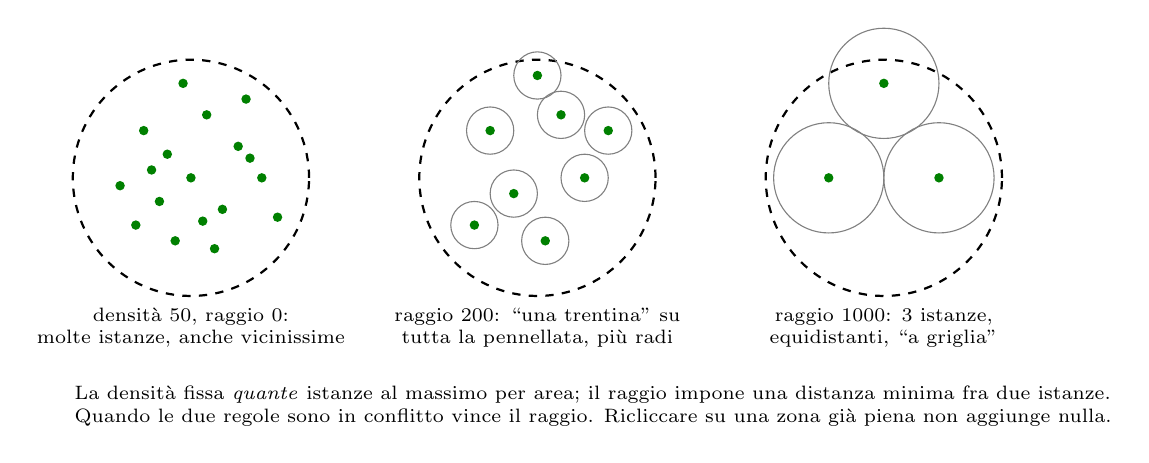
\begin{tikzpicture}[font=\scriptsize, x=1cm, y=1cm]
  % pannello 1: raggio 0
  \draw[thick, dashed] (1.6,1.6) circle (1.5);
  \foreach \p in {(1.0,2.2),(1.3,1.9),(1.8,2.4),(2.2,2.0),(0.7,1.5),(1.2,1.3),(1.6,1.6),(2.0,1.2),(2.5,1.6),(1.4,0.8),(1.9,0.7),(0.9,1.0),(2.3,2.6),(1.5,2.8),(2.7,1.1),(1.1,1.7),(1.75,1.05),(2.35,1.85)}
    {\fill[green!50!black] \p circle (0.06);}
  \node[align=center] at (1.6,-0.3) {densità 50, raggio 0:\\molte istanze, anche vicinissime};
  % pannello 2: raggio medio
  \begin{scope}[xshift=4.4cm]
    \draw[thick, dashed] (1.6,1.6) circle (1.5);
    \foreach \p in {(1.0,2.2),(1.9,2.4),(1.3,1.4),(2.2,1.6),(0.8,1.0),(1.7,0.8),(2.5,2.2),(1.6,2.9)}
      {\fill[green!50!black] \p circle (0.06); \draw[gray] \p circle (0.3);}
    \node[align=center] at (1.6,-0.3) {raggio 200: ``una trentina'' su\\tutta la pennellata, più radi};
  \end{scope}
  % pannello 3: raggio grande
  \begin{scope}[xshift=8.8cm]
    \draw[thick, dashed] (1.6,1.6) circle (1.5);
    \foreach \p in {(0.9,1.6),(2.3,1.6),(1.6,2.8)}
      {\fill[green!50!black] \p circle (0.06); \draw[gray] \p circle (0.7);}
    \node[align=center] at (1.6,-0.3) {raggio 1000: 3 istanze,\\equidistanti, ``a griglia''};
  \end{scope}
  \node[align=left, anchor=west] at (0,-1.3) {La densità fissa \emph{quante} istanze al massimo per area; il raggio impone una distanza minima fra due istanze.\\Quando le due regole sono in conflitto vince il raggio. Ricliccare su una zona già piena non aggiunge nulla.};
\end{tikzpicture}
\caption{Densità e raggio nel Foliage Mode, con i numeri delle prove della lezione. Il
cerchio tratteggiato è il pennello; i cerchi grigi attorno alle istanze rappresentano il
raggio minimo. Ricostruzione schematica: le posizioni dei punti sono indicative.}
\label{ue15:fig:raggio}
\end{figure}

\paragraph{Approfondimento: come piazza il pennello.} Il comportamento visto a lezione è
coerente con il modo in cui il Foliage Mode lavora. A ogni pennellata calcola quante istanze
dovrebbero esserci nell'area del pennello in base a \emph{Density} (istanze per
1000$\times$1000 unità, cioè per 10$\times$10 metri) e alla \emph{Paint Density}; conta quelle
già presenti dello stesso tipo e aggiunge solo le mancanti, scartando ogni posizione
candidata che cada entro il \emph{Radius} di un'istanza esistente. Da qui le tre cose
osservate: ricliccare non aggiunge nulla quando la zona è ``piena''; togliendo il raggio si
riempiono i buchi che il raggio aveva scartato; con un raggio grande la densità teorica non
si raggiunge mai, e le istanze si dispongono a distanza quasi costante. Il raggio è anche il
modo più semplice per evitare alberi compenetrati, il problema che Totten chiama
\emph{casualità percepita} (si veda l'approfondimento della
sezione~\ref{ue15:sec:selezione}). Funzionamento generale dell'engine.

% ---------------------------------------------------------------------
\section{Le altre impostazioni: pendenza, altezza, mobilità, collisioni}
\label{ue15:sec:altre}

\paragraph{Align to Normal e Align Max Angle.} \textbf{Align to Normal} decide se le istanze
``sono allineate alla normal su cui sono applicate''. \textbf{Align Max Angle} è ``quanto si
inclinano per aggiustarsi alla singola pendenza'' (il docente in un primo momento lo confonde
con il parametro successivo e si corregge: ``no, aspetta, mi sa che\dots'').

\paragraph{Ground Slope Angle.} È ``il range in cui il foliage verrà piazzato'': l'angolo
minimo e massimo della superficie su cui un'istanza può comparire. Il docente dipinge l'erba
su un pendio (dopo un momento di confusione: ``stavo modificando ancora le cose dell'albero
invece era l'erba che andava modificata; ci ho cliccato sopra, pensavo di averla selezionata e
invece non era selezionata'', ``è il tipo di cose che vi capiterà sicuramente ogni tanto''). Con
l'intervallo di default, fino a 180, l'erba va ``anche sulla parete rocciosa''. ``Poi sta a voi
decidere se volete che il foliage venga piazzato anche lì oppure no.'' Con un massimo di
\textbf{45} gradi, l'erba compare ``soltanto nelle parti della slope che erano sotto i 47
gradi'' (il docente dice 47 avendo impostato 45: con ogni probabilità è un lapsus), e si
ammucchia nei punti meno ripidi. Abbassando ancora, ``neanche su questa cunetta è stata
messa, perché l'angolazione è troppo alta''. Un uso: mettere attorno alla base del
``montarozzo'' dell'erba a mano, ``per far vedere che un minimo c'è stata un'espansione
erbosa'', senza che salga sulle pareti; ``anche troppo preciso, devo dire''. Il docente lo
rimette a 45 (figura~\ref{ue15:fig:slope}).

\begin{figure}[htbp]
\centering
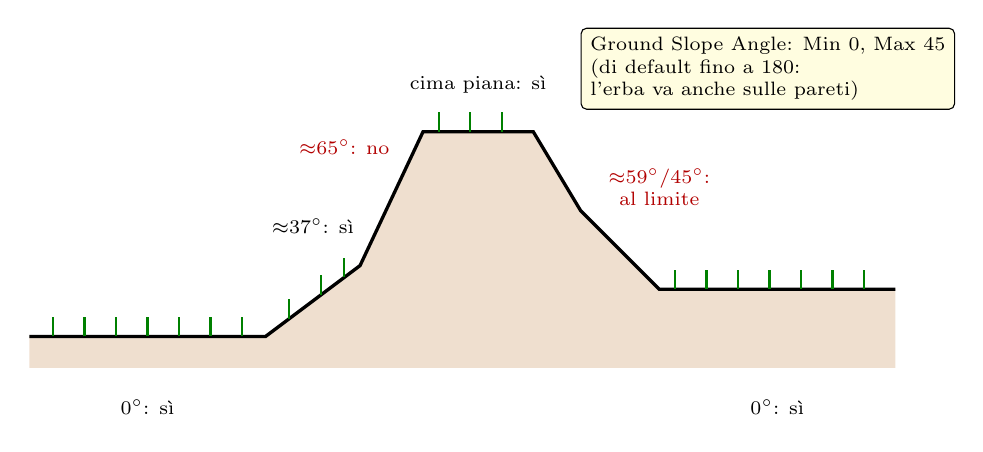
\begin{tikzpicture}[font=\scriptsize, x=1cm, y=1cm]
  \fill[brown!25] (0,0) -- (3,0) -- (4.2,0.9) -- (5.0,2.6) -- (6.4,2.6) -- (7.0,1.6) -- (8.0,0.6) -- (11,0.6) -- (11,-0.4) -- (0,-0.4) -- cycle;
  \draw[very thick] (0,0) -- (3,0) -- (4.2,0.9) -- (5.0,2.6) -- (6.4,2.6) -- (7.0,1.6) -- (8.0,0.6) -- (11,0.6);
  % erba
  \foreach \x in {0.3,0.7,...,2.9} {\draw[green!50!black, thick] (\x,0) -- (\x,0.25);}
  \foreach \x in {3.3,3.7,4.0} {\draw[green!50!black, thick] (\x,{0.75*(\x-3)}) -- (\x,{0.75*(\x-3)+0.25});}
  \foreach \x in {5.2,5.6,...,6.3} {\draw[green!50!black, thick] (\x,2.6) -- (\x,2.85);}
  \foreach \x in {8.2,8.6,...,10.9} {\draw[green!50!black, thick] (\x,0.6) -- (\x,0.85);}
  \node[align=center] at (1.5,-0.9) {0$^\circ$: sì};
  \node[align=center] at (3.6,1.4) {$\approx$37$^\circ$: sì};
  \node[align=center, red!70!black] at (4.0,2.4) {$\approx$65$^\circ$: no};
  \node[align=center] at (5.7,3.2) {cima piana: sì};
  \node[align=center, red!70!black] at (8.0,1.9) {$\approx$59$^\circ$/45$^\circ$:\\al limite};
  \node[align=center] at (9.5,-0.9) {0$^\circ$: sì};
  \node[align=left, anchor=west, draw, rounded corners=2pt, fill=yellow!12] at (7.0,3.4) {Ground Slope Angle: Min 0, Max 45\\(di default fino a 180:\\l'erba va anche sulle pareti)};
\end{tikzpicture}
\caption{Il Ground Slope Angle di un foliage type. Con un massimo di 45 gradi il pennello
piazza istanze solo dove la superficie è inclinata meno di 45 gradi rispetto all'orizzontale;
le pareti restano spoglie. Gli angoli indicati sono esempi. Ricostruzione schematica.}
\label{ue15:fig:slope}
\end{figure}

\paragraph{Height.} Il range d'altezza in cui il foliage può essere piazzato. Di default va
da meno a più infinito (``da meno a più''); con \textbf{0 -- 10}, ``appena andiamo sopra i 10
d'altezza, lui smette di piazzarla''.

\paragraph{Mobility.} Come per le luci: \textbf{Static}, ``più veloci da renderizzare'', che
``funzionano col baking'', o \textbf{Movable}, ``completamente dinamiche'', con le luci che
``reagiscono in tempo reale'', ``ma è più lento da gestire''.

\paragraph{Cull Distance.} ``La distanza massima da cui non smettono di essere renderizzate.''
Allontanandosi, ``tutto il resto del foliage è sparito'', quello del materiale, ``ma questo è
rimasto, perché c'è zero di cull distance'': ``non ha massimo e minimo, esiste e basta, non viene
tagliato, è sempre renderizzato''. ``Gestitelo sulla base della grandezza della vostra scena.''

\paragraph{Le ombre e il dressing.} \emph{Cast Shadow}, ombre dinamiche e statiche,
\emph{Affect Dynamic Lighting}: ``tutti i check che potete gestirvi per la resa estetica con
la luce''. L'erba del pacchetto ``è fatta apposta per non castare ombre''. Il foliage si può
dipingere anche \emph{sopra} le mesh: il docente mette dell'erba sopra una struttura della
base, e immagina ``un mondo post apocalittico con una pompa di benzina abbandonata'' (``non so
perché mi ha fatto pensare alla pompa di benzina''), con l'erba che ci cresce sopra e ``dei
\emph{vine} che scendono giù'' (delle liane, dei rampicanti).

\paragraph{Collision Presets.} ``E poi abbiamo i preset delle collisioni.'' La frase del docente
è ambigua (``di default tutto il foliage è impostato a una collisione, che nel caso dell'erba
ci fa anche comodo, perché noi non vogliamo che ci sia l'erba e poi ci inciampiamo sopra''):
il senso è che \emph{per l'erba} si vuole che non ci siano collisioni. ``Quando andiamo a
mettere gli alberi, però, dobbiamo assicurarci che lì sia tutto funzionale, che le collisioni
ci siano, perché altrimenti possiamo passarci attraverso.''

\paragraph{L'ingresso della base.} Prima degli alberi il docente sistema l'erba davanti alla
base: ``il nostro personaggio uscirà da lì e si trova prima l'erbetta che va a gradiente, poi
c'è il folto''.

\paragraph{Approfondimento: le impostazioni del foliage type.} Qualche precisazione sui
parametri visti. \emph{Ground Slope Angle} confronta la normale della superficie con la
verticale, come il World Aligned Blend dell'automaterial: le due cose si possono far
coincidere, così che il foliage manuale non finisca dove il materiale mette la roccia.
\emph{Height} usa la quota assoluta del mondo in centimetri, quindi ``0 -- 10'' è una fascia di
dieci centimetri sopra lo zero del mondo, utile per esempio per non piantare canne sopra il
livello dell'acqua. \emph{Cull Distance} ha un minimo e un massimo: fra i due le istanze
sfumano, e con entrambi a 0 il culling per distanza è disattivato, come visto. I
\emph{Collision Presets} del foliage type (\emph{Body Instance}) decidono come le istanze
\emph{rispondono} alle collisioni; perché ci sia una collisione, però, la mesh deve averne una
(la sezione successiva lo mostra). Romero e Sewell descrivono nel capitolo 14 (``Math and
Trace Nodes'') la tabella delle \emph{Collision Responses}: ogni oggetto ha un \emph{Object
Type} e una risposta (\emph{Ignore}, \emph{Overlap} o \emph{Block}) per ogni canale, con dei
preset come \emph{BlockAll}, \emph{OverlapAllDynamic} e \emph{Pawn}, oppure
\emph{Custom\ldots}; nel capitolo 5 impostano \emph{BlockAllDynamic} su un oggetto
interattivo. Le stesse regole valgono per le istanze del foliage.

% ---------------------------------------------------------------------
\section{Gli alberi e le collisioni}
\label{ue15:sec:alberi}

\paragraph{Le impostazioni dell'albero.} ``Togliamo l'erba, perché sennò dipingiamo anche
l'erba insieme agli alberi.'' Le impostazioni del pacchetto: \textbf{Density 1}, ``abbastanza
sparsi'', raggio 0: ``ci può stare''. Il docente ne mette una fila all'ingresso, ``una piccola
radura''. Gli alberi sono di taglie diverse (\textbf{Scale} da 1 a 3: ``con l'albero funziona
meglio, dà un'idea migliore''; c'è l'albero ``di base'' e ``l'albero grosso'') e ruotati in
maniera diversa: lo Z Offset è 0, ma c'è il \textbf{Random Yaw}, ``una rotazione randomica
sull'asse verticale''. Togliendolo, ``gli alberi vanno tutti nella stessa direzione, sono tutti
curvi in quella direzione, verso sinistra''; rimettendolo, ``iniziano a ruotare''. (Un albero
``si è rifiutato di essere cancellato''.)

\paragraph{Alberi dalle pareti.} Lasciando il Ground Slope Angle ampio e Align to Normal
attivo, si possono piantare alberi su una parete: ``alberi che escono dalle pareti, non so
perché dovreste volerlo fare, ma lo potete fare''. Per esempio ``un percorso di alberi tutto
attaccato sul lato della parete, che potete utilizzare come percorso per un platform''.
Togliendo Align to Normal ``ve li spawna dritti''. Con gli alberi l'allineamento ``non funziona
granché bene'', ``ma per esempio con dei cespugli o dei funghi parassiti'' sì.

\paragraph{La collisione strana.} Le collisioni dell'albero sono \textbf{Block All}. ``Col
nostro robottino andiamo all'avventura'': ``siamo alti quanto l'erba'' (bisognerà abbassarla).
In Play si riesce a passare dentro gli alberi, almeno in parte: ``hanno una strana
collisione''. Prima di guardare, il docente chiarisce ``una grossa cosa'' sulle collisioni:
``questo parametro non determina se l'oggetto avrà collisioni o meno; determina se le
collisioni dell'oggetto sono attive o meno, e per cosa sono attive''. La prova: Block All
sull'\textbf{erba}. ``Sono positivamente sicuro che potremo comunque camminare dentro l'erba'':
ed è così (``se dovessimo esplorare un open world del genere, il nostro personaggio dovrebbe
muoversi più veloce di così''). Il motivo è nella static mesh di base: nello Static Mesh
Editor, con \textbf{Show Simple Collision}, ``non ci sono simple collision, quindi non c'è
nulla da attivare''. ``Vi capiterà di mettere degli asset in scena, iniziare a giocare e
passarci attraverso, perché magari quegli asset sono stati importati o esportati senza le
collisioni''; e anche impostando ``le collisioni che bloccano tutto, o che bloccano solo i
proiettili'', ``lui comunque non può bloccare, perché non c'è nulla da bloccare''.

\paragraph{L'albero, dentro.} Aprendo la mesh dell'albero: ``ah, geniale. L'hanno messa dalla
parte sbagliata.'' Le forme della collisione semplice (``diversi pezzi'') sono ruotate rispetto
al tronco, ``credo che l'abbiano importato proprio con la collisione sbagliata''. Si possono
selezionare tutte e ruotare ``dalla parte corretta''; ``anche se sono proprio strane'',
sbagliate anche nelle proporzioni. Tre strade:
\begin{enumerate}
  \item \textbf{ruotare} le forme esistenti, come fa il docente (``tanto il nostro giocatore
        non andrà mai a collidere lassù, a meno che non vogliamo che lo faccia'');
  \item \textbf{eliminare} le simple collision e scegliere \textbf{Use Complex Collision As
        Simple}: la collisione prende ``esattamente i poligoni dell'albero''. ``Chiaramente
        questa cosa è pesante, però vi risolve il problema di dover fare le collisioni a
        mano'';
  \item \textbf{rifarle} a mano con forme semplici: ``vi basterebbe prendere un cilindro,
        metterlo in diagonale, e qui sopra metterci un piano circolare''. Il docente aggiunge
        una \textbf{capsula}, la fa più piccola e più stretta, la ruota lungo il tronco, e
        sopra una \textbf{box piatta}, ``in modo che il giocatore possa salire sulla cima
        dell'albero e rimanerci sopra'' (figura~\ref{ue15:fig:collisione}).
\end{enumerate}
Se si vuole che il personaggio salti da un albero all'altro o percorra la parete passando sui
tronchi, ``non potete fare questa cosa'' con la collisione originale: ``dovete togliere queste
collisioni e rifarle''.

\begin{figure}[htbp]
\centering
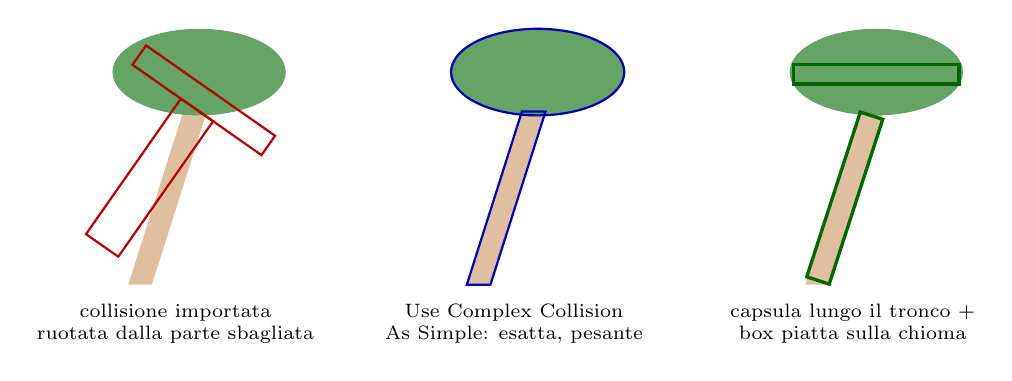
\begin{tikzpicture}[font=\scriptsize, x=1cm, y=1cm]
  % albero originale
  \begin{scope}
    \fill[brown!50] (0.9,0) -- (1.2,0) -- (1.9,2.2) -- (1.6,2.2) -- cycle;
    \fill[green!40!black!60] (1.8,2.7) ellipse (1.1 and 0.55);
    \draw[red!70!black, thick, rotate around={-35:(1.2,1.4)}] (0.95,0.3) rectangle (1.45,2.4);
    \draw[red!70!black, thick, rotate around={-35:(1.2,1.4)}] (0.2,2.4) rectangle (2.2,2.7);
    \node[align=center] at (1.5,-0.5) {collisione importata\\ruotata dalla parte sbagliata};
  \end{scope}
  % complex as simple
  \begin{scope}[xshift=4.3cm]
    \fill[brown!50] (0.9,0) -- (1.2,0) -- (1.9,2.2) -- (1.6,2.2) -- cycle;
    \fill[green!40!black!60] (1.8,2.7) ellipse (1.1 and 0.55);
    \draw[blue!70!black, thick] (0.9,0) -- (1.2,0) -- (1.9,2.2) -- (1.6,2.2) -- cycle;
    \draw[blue!70!black, thick] (1.8,2.7) ellipse (1.1 and 0.55);
    \node[align=center] at (1.5,-0.5) {Use Complex Collision\\As Simple: esatta, pesante};
  \end{scope}
  % capsula + box
  \begin{scope}[xshift=8.6cm]
    \fill[brown!50] (0.9,0) -- (1.2,0) -- (1.9,2.2) -- (1.6,2.2) -- cycle;
    \fill[green!40!black!60] (1.8,2.7) ellipse (1.1 and 0.55);
    \draw[green!40!black, very thick, rotate around={-18:(1.4,1.1)}] (1.25,0.0) rectangle (1.55,2.2);
    \draw[green!40!black, very thick] (0.75,2.55) rectangle (2.85,2.8);
    \node[align=center] at (1.5,-0.5) {capsula lungo il tronco +\\box piatta sulla chioma};
  \end{scope}
\end{tikzpicture}
\caption{Tre modi di sistemare la collisione dell'albero di StackOBot visti a lezione:
ruotare le forme importate male, usare la geometria della mesh come collisione, oppure
rifare la collisione con una capsula (qui disegnata come un rettangolo inclinato) e una box
piatta su cui il giocatore può stare in piedi. Ricostruzione schematica.}
\label{ue15:fig:collisione}
\end{figure}

\paragraph{La domanda sulle collisioni a senso unico.} Uno studente ha una domanda ``fuori
tema'': ``le collisioni che funzionano da un solo lato?'' Gli è venuto in mente un gioco (``PIC''
nella trascrizione: con ogni probabilità \emph{PEAK}, il gioco cooperativo di arrampicata, ma
il nome non è certo) in cui ``puoi salire sugli alberi e puoi attraversare le foglie da sotto,
ma non puoi attraversarle da sopra''. Il docente non ci ha mai pensato: ``probabilmente dipende
dal modo in cui è codificato quel tipo di interazione''. ``Gli dici che se stai andando in una
direzione non deve contare quella collisione, se stai andando nell'altra deve contarla.
Penso, non lo so, a naso direi che è questo.'' Non ha giocato il gioco.

\paragraph{No Collision sovrascrive.} Rimesso tutto com'era, con le collisioni girate ``dalla
parte giusta'', il docente imposta \textbf{No Collision} nel foliage type dell'albero: ``lui
sovrascrive il fatto che ha delle collisioni''. In Play ci si passa attraverso, ``perché l'asset
del foliage non ha collisioni''. Con \textbf{Custom} si sceglie che cosa bloccano: ``se bloccano
la camera, se bloccano i proiettili, se bloccano il pawn''. ``Di base, il Block All andrà
bene.''

\paragraph{Approfondimento: collisione semplice, complessa e a senso unico.} Una static mesh
ha due rappresentazioni di collisione. La \emph{simple collision} è fatta di primitive
(box, sfere, capsule, convessi) ed è quella usata dalla fisica e dal movimento del
personaggio: è economica, ma va costruita (nello Static Mesh Editor, menu
\emph{Collision}: \emph{Add Box}, \emph{Add Capsule}, \emph{Auto Convex Collision}\dots)
o importata dal programma di modellazione. La \emph{complex collision} è la mesh stessa,
triangolo per triangolo, usata di solito solo per le tracce precise. \emph{Collision
Complexity: Use Complex Collision As Simple} fa usare la seconda anche per la fisica: comoda,
ma costosa su mesh dense e, per i corpi simulati, non utilizzabile. Le collisioni ``a senso
unico'' delle piattaforme attraversabili da sotto non sono una proprietà della collisione
in Unreal: si ottengono via codice, per esempio con un volume sotto la piattaforma che, quando
il personaggio sale, gli fa ignorare il canale della piattaforma (\emph{Ignore}) e lo
ripristina quando il personaggio è sopra, oppure controllando la velocità verticale; è
proprio la risposta ``a naso'' del docente. Le risposte \emph{Ignore}/\emph{Overlap}/\emph{Block}
per canale sono quelle della tabella del capitolo 14 di Romero e Sewell; il resto è
funzionamento generale dell'engine.

% ---------------------------------------------------------------------
\section{Selezionare, rifinire e il foliage non naturale}
\label{ue15:sec:selezione}

\paragraph{Il cespuglio a mano.} ``Lo stesso con gli altri oggetti.'' Il cespuglio del
pacchetto spawna poco; è ``un tipo di asset che io, piuttosto che metterlo così, farei
\textbf{single} e andrei a posizionare a mano'': ``voglio che queste cose stiano molto
ammucchiate vicino agli alberi''. Le dimensioni sono comunque casuali, ``forse troppo varie
per i miei gusti''. Allo stesso modo si fa ``un percorso alberato'', con alberi a destra e a
sinistra, che ``fa comunque parte del foliage'' e si integra con il resto.

\paragraph{Gli strumenti di selezione.}
\begin{itemize}
  \item \textbf{Select}: si prende ``il singolo pezzo di foliage'' e lo si sposta (``no, no,
        quest'albero non deve stare proprio lì, deve stare qui''), ``un po' tipo selection mode,
        ma con tutti gli asset che rimangono all'interno del foliage''. Tornando in Selection
        Mode e cliccando, invece, si seleziona tutto il foliage actor. (Il docente trova
        nell'Outliner anche delle istanze che non si aspettava, ``saranno delle cose che
        c'erano prima'', e non approfondisce.)
  \item \textbf{Select All} e \textbf{Deselect}: tutte le istanze dei tipi attivi, da
        muovere insieme.
  \item \textbf{Select Invalid}: ``mi porta automaticamente alle instance che sono invalide,
        quindi quelle che vanno modificate''.
  \item \textbf{Lasso}: ``funziona un po' tipo Photoshop'': invece di cliccare, si evidenzia
        una zona. Vale solo per i tipi spuntati: ``qui ci sono sempre attivi soltanto gli
        alberi, quindi se voglio fare questa cosa devo prendere anche questi''.
  \item \textbf{Remove}: ``questi alberi qua non mi piacciono'': elimina tutto ciò che è stato
        evidenziato.
  \item un ultimo strumento, ``stessa cosa con i raise, però è un discorso un po' diverso, poi
        modifica piano piano'': il nome non è ricostruibile con certezza (con ogni probabilità
        \emph{Reapply}, che riapplica le impostazioni del foliage type alle istanze già
        dipinte).
\end{itemize}

\paragraph{Non deve essere naturale.} ``È tendenzialmente uno strumento che utilizzate
principalmente per motivi estetici.'' E ``non deve essere necessariamente naturale'': si può
usare ``con ogni mesh che voglio''. ``Se io voglio riempire la scena di robottini, lo posso
fare''; una scena in metropolitana con il pavimento pieno di ``cartacce, plastiche, cose
varie''. ``È un po' un pennello con cui piazzare rapidamente tutta una serie di oggetti.''

\paragraph{Le rocce sotto lo zero.} Le rocce dipinte ``appena si avvicinano allo zero
impazziscono; invece sopra sono perfette''. Consiglio: ``mettete il piano di base leggermente
più alto dello zero''. Spostando una roccia, il materiale cambia: ``cambia sulla base
dell'altezza''; ruotandola, ``così diventa una parete rocciosa''. ``È un po' strano che abbiano
scelto di fare un materiale dinamico così per un oggetto standard.'' Aprendo il materiale
(``più complesso di quello che pensavo''), il docente legge nomi come \emph{Virtual
Texture}, \emph{World Position} e una ``variation'' (la trascrizione dice ``part time, drop
variation'', non ricostruibile): ``hanno provato a fare una roba carina'' per avere un
materiale dinamico, ``tipo il \textbf{vertex painting}'', e per ``blendare la mesh con
l'oggetto del landscape'' quando si dipinge il materiale del landscape. Ma ``volendo, potete
fare anche letteralmente solo una texture di roccia'' con le sue mappe, ``e avete comunque una
roccia''.

\paragraph{Approfondimento: la casualità percepita.} Il Foliage Mode rende facilissimo
spargere oggetti a caso, ed è proprio il rischio che Totten descrive nel capitolo 8
(``Possibility Spaces and Worldbuilding''): in natura alberi, rocce e scogliere si dispongono
nel tempo in modi non pianificati, e i designer alle prime armi piazzano alberi, rocce ``e
perfino edifici'' a caso sulla mappa, ``ignari dell'importanza della loro posizione''; il
risultato è una \emph{casualità percepita} che non dice nulla al giocatore. ``Dirigere lo
sguardo verso elementi scenici piazzati con cura'' è il modo in cui il giocatore capisce il
mondo. In pratica: il pennello per la massa (l'erba, il bosco di sfondo), lo \emph{Single
Instance Mode} e il \emph{Select} per gli elementi che contano (l'albero isolato che fa da
landmark, i cespugli che incorniciano un passaggio), che è esattamente il modo di lavorare del
docente con i cespugli. Nel capitolo 3 (``Basic Gamespaces'') Totten aggiunge che un cambio
nel tipo di vegetazione segnala il passaggio a una zona nuova, come un cambio di texture sul
terreno. Sul materiale delle rocce: un materiale che campiona texture in world space
(\emph{world aligned}) cambia aspetto quando l'oggetto si sposta o ruota, perché la texture
resta ferma nel mondo mentre la mesh si muove; e un calcolo basato sulla quota assoluta (per
esempio per sfumare la base nella sabbia o nell'umidità) produce effetti strani sotto lo
zero, se chi l'ha fatto ha supposto che il terreno stia sopra. Funzionamento generale
dell'engine; il grafo del materiale non è stato verificato nel capitolo.

% ---------------------------------------------------------------------
\section{La domanda sui mondi procedurali}
\label{ue15:sec:procedurale}

\paragraph{Landscape o mesh?} ``Ci sono domande?'' Uno studente: ``i mondi che si generano
automaticamente usano il landscape o le mesh?'' ``Tipo le robe procedurali? Tendenzialmente
dipende.'' ``È più comodo farlo con le mesh, perché puoi farti un \textbf{array} di oggetti e
puoi piazzarli secondo dei criteri che hai scelto tu.'' Ma ``l'ultima volta che ho lavorato
con qualcosa di procedurale era un sacco di tempo fa'', e magari ci sono ``nuovi nodi'' o
``feature che Unreal ha inserito'' che il docente non conosce. Il consiglio: cercare sullo store
``qualche pacchetto che parla di asset procedurali, non modulari, proprio procedurali, che ha
dei sistemi di proceduralizzazione'', e ``ti studi un po' loro come le fanno''. ``Fab, intendi,
giusto?'' ``Sì, su Fab. Ai miei tempi non si chiamava Fab, mi sento vecchio.''

\paragraph{Lo strumento che non si trova.} Parlando di procedurale, il docente ricorda ``un
tool che io non ho mai usato, che dovrebbe essere relativamente nuovo'': ``una specie di box
all'interno della quale possono essere impostati dei parametri, e spostando questa box e
ingrandendola, lui va a piazzare quel tipo di foliage nel volume che c'è all'interno''. Lo
cerca fra i tipi di asset del menu \emph{Foliage} (c'è lo \emph{Static Mesh Foliage}, ``questo
qui è letteralmente il nuovo, ma non è quello che voglio''), non lo trova, e ipotizza che
fosse ``un plugin''. ``Me lo devo vedere meglio.''

\paragraph{Sprite e flipbook.} Nello stesso menu ``vi potete vedere tutti i tipi di asset che
possono essere creati'', anche gli \textbf{sprite} e i \textbf{flipbook}: ``carini se volete
fare, che ne so, un menu animato''. ``Visto che avete fatto la roba col menu, con un flipbook
potete andare a fare l'animazione del menu.''

\paragraph{Approfondimento: generazione procedurale in Unreal.} Lo strumento descritto dal
docente corrisponde con ogni probabilità a uno di due sistemi, ed entrambi si attivano da
plugin. Il primo è il \emph{Procedural Foliage Spawner} con il suo \emph{Procedural Foliage
Volume}: si definisce quali foliage type crescono, con quali regole di competizione e di
età, e si fa ``simulare'' la crescita dentro il volume (è una funzione sperimentale,
\emph{Procedural Foliage}, da abilitare nelle impostazioni dell'editor). Il secondo, più
recente e oggi il sistema di riferimento, è il framework \emph{PCG} (\emph{Procedural
Content Generation}), con il \emph{PCG Volume} e un grafo a nodi che campiona superfici,
filtra i punti per pendenza o altezza e vi genera mesh: il plugin si chiama
\emph{Procedural Content Generation Framework}. La risposta del docente sulle mesh resta
valida: anche il PCG, alla fine, produce istanze di static mesh. Romero e Sewell, nel
capitolo 19 (``Procedural Generation''), definiscono la generazione procedurale come ``un
metodo per creare il contenuto del livello usando script invece che a mano'', utile per
evitare compiti ripetitivi; la costruiscono con il \emph{Construction Script}, un
\emph{Instanced Static Mesh Component} e dei cicli \emph{For Loop} che dispongono righe di
istanze, e poi con le \emph{Blueprint Spline} per piazzare actor lungo un percorso. Gli
sprite e i flipbook appartengono a \emph{Paper2D}, il sistema 2D dell'engine: un flipbook è
una sequenza di sprite riprodotta a una certa velocità. Fab è lo store di Epic che dal 2024
ha sostituito l'Unreal Engine Marketplace, quello usato nel capitolo 9 del libro per
importare l'\emph{Animation Starter Pack}.

% ---------------------------------------------------------------------
\section{Il Niagara e il Post Process Volume}
\label{ue15:sec:postprocess}

``Come ho detto, ci abbiamo una decina di minuti.'' In quella decina di minuti si potrebbe
``buttare un occhio'' sul post process, ``visto che ci siamo''.

\paragraph{Un'occhiata al Niagara.} Prima, ``al volo'', il Niagara: ``è proprio un editor a
parte''. Creando un \textbf{Niagara System} si sceglie fra ``tutte le varie forme, modi, colori,
possibilità'' dei \emph{preset}; il docente prende una \textbf{Fountain}, ``la base della
cosa''. Dentro c'è ``tutto un sistema così, con la timeline, con degli \textbf{emitter}, tutte
cose''. ``È una roba un po' complicata, magari ce la vediamo alla prossima lezione se
riusciamo.''

\paragraph{Dove si trova il post process.} Dal \textbf{Place Actors}, nella categoria
\textbf{Volumes}, ``tra le varie cose'' (``insieme a tutta una serie di altre cose molto, molto
carine'') c'è il \textbf{Post Process Volume}: ``il nostro quadratone''.

\paragraph{Che cos'è.} ``È un volume all'interno del quale voi andate ad applicare delle
modifiche alla lente della telecamera, fondamentalmente.'' ``Voi andate a modificare il modo in
cui le cose appaiono, non il modo in cui le cose sono.'' Le stesse ``lenti'' esistono anche su
una \textbf{Camera Actor}: nei suoi Details, nella sezione \emph{Post Process}, ``abbiamo
diverse lenti che possiamo andare a modificare'', e queste modifiche ``si applicano solo alla
singola telecamera''. Il volume invece applica gli effetti \emph{al suo interno}.

\paragraph{Le transizioni.} ``Vi siete mai chiesti come fanno a fare quegli effetti per cui
quando entri o esci da una casa il bloom della luce è particolarmente forte e poi si attenua?
O com'è possibile che la luce fuori era molto forte, io entro dentro una grotta e piano piano
la luce diventa più tenue e cambia colore?'' ``È perché il post process ha degli effetti di
transizione fra l'interno e l'esterno.'' Si possono piazzare più Post Process Volume con
effetti diversi, e passando dall'uno all'altro cambia ``il modo in cui la mia telecamera va a
gestire le cose''.

\paragraph{I volumi annidati.} Si può anche mettere un post process dentro un altro, ``una roba
complicata che vi sconsiglierei di fare'': il volume interno ``calcola tutto quello che lui
deve calcolare e in più ci applica anche quello'' dell'esterno. L'esempio: il volume interno
rende la scena gialla (\emph{color correction}), quello esterno blu; stando nell'interno ``vediamo
tutto verde, perché lui somma la color correction dei due post process''. ``Per cui diventa molto
complicato capire cosa vogliamo fare.'' (Figura~\ref{ue15:fig:postprocess}.)

\paragraph{Un solo volume per tutto: Infinite Extent.} ``Se voglio un unico post process che
determina il modo in cui la scena viene vista, devo renderlo incredibilmente grande?'' No:
nei Details del volume (``le stesse lenti che aveva il camera actor, con qualche opzione in
più'') si cerca \emph{infinite} e si trova \textbf{Infinite Extent (Unbound)}: ``quando questa
casella viene spuntata, il volume copre tutto il mondo, non solo l'area all'interno'', e i
cambiamenti ``vengono visti allo stesso modo in tutta la zona''. Per ora la si toglie.

\paragraph{Le lenti, per la prossima volta.} ``Non so quanto senso abbia iniziare a parlare
delle lenti: ci abbiamo 5 minuti, e ogni lente ha un sacco di parametri.'' Due accenni: il
\textbf{Bloom}, ``abbastanza semplice'', ``quello che serve per i god shaft'' di cui si parlava
prima; e la \textbf{Chromatic Aberration}: ``occhio, che fa male agli occhi''. Il resto alla
prossima lezione.

\begin{figure}[htbp]
\centering
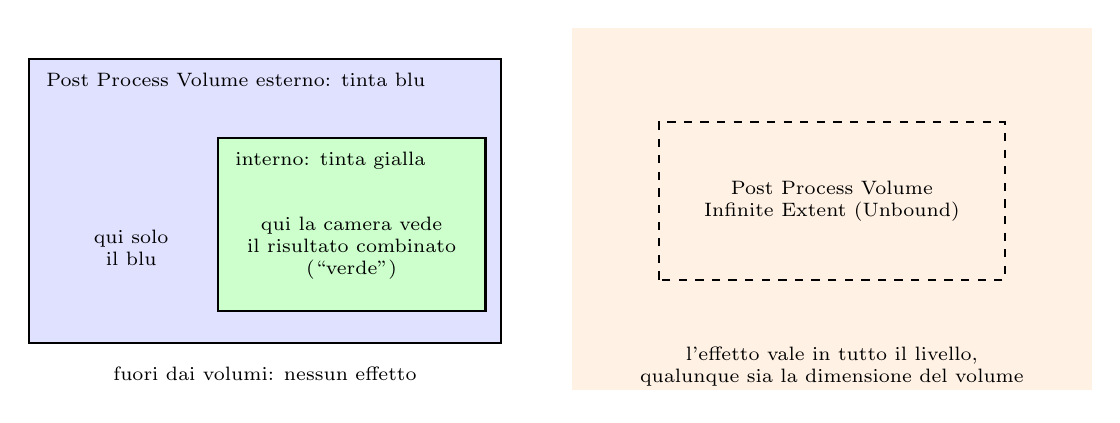
\begin{tikzpicture}[font=\scriptsize, x=1cm, y=1cm]
  \draw[thick, fill=blue!12] (0,0) rectangle (6,3.6);
  \node[anchor=north west] at (0.1,3.55) {Post Process Volume esterno: tinta blu};
  \draw[thick, fill=green!20] (2.4,0.4) rectangle (5.8,2.6);
  \node[anchor=north west, align=left] at (2.5,2.55) {interno: tinta gialla};
  \node[align=center] at (4.1,1.2) {qui la camera vede\\il risultato combinato\\(``verde'')};
  \node[align=center] at (1.3,1.2) {qui solo\\il blu};
  \node[align=center] at (3,-0.4) {fuori dai volumi: nessun effetto};
  % unbound
  \begin{scope}[xshift=7.2cm]
    \fill[orange!10] (-0.3,-0.6) rectangle (6.3,4.0);
    \draw[thick, dashed] (0.8,0.8) rectangle (5.2,2.8);
    \node[align=center] at (3,1.8) {Post Process Volume\\Infinite Extent (Unbound)};
    \node[align=center] at (3,-0.3) {l'effetto vale in tutto il livello,\\qualunque sia la dimensione del volume};
  \end{scope}
\end{tikzpicture}
\caption{A sinistra, due Post Process Volume annidati: dentro il volume interno la camera
riceve l'effetto di entrambi, come nell'esempio del docente (giallo e blu che danno verde). A
destra, un volume con \emph{Infinite Extent (Unbound)}, che vale per tutto il livello.
Ricostruzione schematica.}
\label{ue15:fig:postprocess}
\end{figure}

\paragraph{Approfondimento: come si combinano i post process.} Il comportamento dei volumi
sovrapposti è un po' più ordinato della ``somma'' descritta a lezione. Ogni Post Process
Volume ha una \emph{Priority}, un \emph{Blend Weight} (da 0 a 1) e un \emph{Blend Radius}, la
distanza dal bordo entro cui l'effetto sfuma: è il Blend Radius che produce le transizioni
graduali fra esterno e grotta. Ogni volume modifica solo le proprietà la cui casella è
spuntata; quando la camera è dentro più volumi, Unreal li applica in ordine di priorità, e
per ogni proprietà il valore del volume a priorità più alta si \emph{mescola} con quello già
calcolato secondo il suo Blend Weight (con peso 1 lo sostituisce). Se due volumi cambiano
proprietà diverse, si vedono entrambe le modifiche; se cambiano la stessa con peso minore di
1, si ottiene una via di mezzo: in questo senso le due tinte possono dare un colore
combinato. Il consiglio del docente resta buono: pochi volumi, priorità esplicite, e di solito
un volume \emph{Unbound} a priorità bassa per l'aspetto generale del livello più volumi locali
per le zone speciali. Le impostazioni della Camera Actor (e del \emph{Camera Component} del
personaggio) si combinano con quelle dei volumi, con un proprio peso. Romero e Sewell, nel
capitolo 9 (``Building Smart Enemies with Artificial Intelligence''), allargando l'area di
gioco ricordano che il \emph{PostProcessVolume} e il \emph{LightmassImportanceVolume} ``devono
coprire la nuova area di gioco'', perché ``questi volumi sono usati per l'illuminazione e gli
effetti''; nel capitolo 12 indicano la qualità del \emph{Post Processing} (filtri come motion
blur e bloom applicati allo schermo dopo il rendering della scena) fra le impostazioni da
ridurre se le prestazioni sono basse. Il resto è funzionamento generale dell'engine.

% ---------------------------------------------------------------------
\section{I compiti, la vetrata colorata e la chiusura}
\label{ue15:sec:chiusura}

\paragraph{Il compito.} ``Visto che le cose principali che abbiamo visto in queste due lezioni
sono sicuramente il landscape e sicuramente il foliage'', il compito per il fine settimana,
``come abbiamo fatto settimana scorsa con la gym e il livello'':
\begin{itemize}
  \item in un altro livello, o nello stesso, ``un piccolo spazio'': un piccolo landscape con
        il suo foliage, ``che abbia un'estetica abbastanza curata'' (``gli oggetti che avete a
        disposizione sono pochi, quindi non potete fare troppa roba'');
  \item che \textbf{circondi la vostra gym}, ``il posto in cui avete messo le cose'', e in cui
        il personaggio ``possa muoversi un po', girovagare''; conviene aumentare un po' la
        velocità di movimento del personaggio;
  \item lo scopo: ``un piccolo livellino di \textbf{esplorazione} utilizzando il landscape''.
        ``Nulla di troppo complesso'': magari ``delle pedane che vi fanno salire e scendere da
        una parte all'altra''; come la volta scorsa, ``un paio di \textbf{collezionabili} in
        giro''; ``delle alture, degli avvallamenti'', e ``se ve la sentite particolarmente
        creativi, anche dei buchi, delle grotticine'';
  \item ``potete mettere in pratica il fatto di dover saltare sugli alberi, se volete'':
        sistemate le collisioni e via.
\end{itemize}
(Nel mostrarlo, il docente alza un pezzo di terreno e ``clippa'' tutto: ``adesso sono sul
cane'', cioè, con ogni probabilità, sotto o dentro la geometria; ``siamo direttamente sulla
sabbia''.)

\paragraph{Le dimensioni.} ``Chiaramente non deve essere una mappa così grande.'' Il docente
ragiona ad alta voce: ``15 per 15 va piccolino'', ``\textbf{31 per 31} conviene, che avete
abbastanza spazio per fare un po' di cose''. (La trascrizione non dice a che cosa si
riferisca il numero; 31 per 31 è uno dei valori della \emph{Section Size} visti nella lezione
precedente, ma potrebbe anche indicare il numero di quad del landscape. In ogni caso il
senso è: un landscape piccolo.) Si può usare il materiale costruito insieme e ``sbizzarrirsi
un pochino'', ``costruire qualcosina''.

\paragraph{Il video.} ``Se volete potete anche mettere un video di voi che camminate in
quell'ambiente su Discord'': si registra e lo si carica. Uno studente che non ci sarà
all'ultima lezione: ``io penso che farò così''. ``Va benissimo: è comunque una testimonianza del
fatto che fate cose. Magari ispirate gli altri.'' Vale anche per i livelli e le gym della
volta scorsa. ``Fateli poco pesanti però, perché Discord mi sa che non vi permette di caricare
troppa roba''; altrimenti si mettono su un Drive e si condivide il link.

\paragraph{La domanda sul volume.} Lo studente che mancherà all'ultima lezione chiede del post
process: ``la lente funziona nel momento in cui stai dentro l'area, o funziona attraverso, se
guardi attraverso?'' ``Dentro'': ``è un volume, è come un trigger volume, come un blocking
volume; funziona nel momento in cui tu sei all'interno del volume''. Se si vuole una stanza di
un colore, ``devi mettere il post process tutto attorno all'ambiente''.

\paragraph{La vetrata colorata.} ``Ma quindi, per esempio, una finestra colorata che trasforma
la luce in luce colorata usa le lenti o qualcos'altro?'' ``Usa un po' di entrambi,
tendenzialmente. Quando ti fai questa domanda, la risposta è sempre: entrambi.'' L'esempio è la
\textbf{vetrata di una chiesa}:
\begin{enumerate}
  \item un oggetto con un \textbf{materiale di vetro}, ``che permetta di vedere attraverso'' e
        ``del giusto colore per dare quell'idea'';
  \item una \textbf{luce forte} proiettata attraverso, con il colore cambiato ``in modo che la
        luce sia di quel colore lì'';
  \item il \textbf{post process} ``per accentuare l'effetto di cambio della luce''.
\end{enumerate}
E se la directional light deve restare bianca, vista da fuori, ma colorata da dentro? Allora
``senza cambiare la luce'': il materiale del vetro ``che comunque filtra un pochino la luce'', e
il post process che, mentre sei dentro, cambia il colore percepito. ``Ah, è una specie di
escamotage.'' ``È tutto un escamotage.'' ``Costruire livelli diventa sempre tipo trovare il
\textbf{trucchetto del mago} per ingannare la persona.'' Si potrebbe certo fare in modo che
``nel momento in cui la luce attraversa quel determinato trigger il calcolo del colore della
luce cambi'', ``però è sicuramente più complicato e più dispendioso che fare un trucchetto''.

\paragraph{La chiusura.} Domande e lavori si possono mettere sul Discord. ``La prossima lezione,
sicuramente, vi parlo al volo del \textbf{packaging}'': ``così, oltre a fare il video, magari
possiamo proprio fare un eseguibile che può essere passato e può essere giocato anche dagli
altri''. ``Buon fine settimana, buona serata. E ci vediamo martedì prossimo.''

\paragraph{Approfondimento: la luce attraverso il vetro.} In Unreal Engine~5 una luce non
cambia colore da sola attraversando un materiale traslucido: le ombre dei materiali
\emph{translucent} sono di norma solo più o meno scure, non colorate. Per questo il ``trucco del
mago'' del docente è la strada pratica: una \emph{spot light} o una \emph{rect light} colorata
dietro la vetrata, eventualmente con una \emph{Light Function} (un materiale che maschera la
luce con il disegno della vetrata) per proiettare il motivo sul pavimento, un cono finto come
quelli dell'engine per il fascio, e un Post Process Volume nella navata per la tinta
generale. Totten, nel capitolo 5 (``Introducing Emotional Level Design through Survival
Instincts''), parla proprio di questa luce: l'\emph{ombra} (\emph{shade}) ottenuta facendo
entrare luce diffusa attraverso tende, schermi o vetrate fu un tratto centrale
dell'architettura gotica, che cercava un'esperienza eterea chiamata \emph{lux nova}, ``luce
nuova'' o ``luce mistica''; e la stessa condizione, con la nebbia, è un caposaldo dell'horror.
Nel capitolo 1 ricorda che le vetrate gotiche ``filtravano la luce nella chiesa per creare
un'atmosfera che facesse sentire i fedeli più vicini a Dio''. Nello stesso capitolo 5 Totten
riprende Christopher Alexander: la luce posta agli incroci di un percorso \emph{attira} le
persone in quella direzione. I god rays della directional light e i coni finti sono, in
questo senso, strumenti di guida, non solo di estetica. Sul packaging annunciato, Romero e
Sewell (capitolo 12, ``Building and Publishing'') descrivono il procedimento:
\emph{Platforms} $\rightarrow$ piattaforma $\rightarrow$ \emph{Package Project}, la scelta
della cartella, la finestra del log in caso di errori e le \emph{Packaging Settings}, con la
\emph{Build Configuration} e la \emph{Staging Directory}.

% ---------------------------------------------------------------------
\begin{table}[htbp]
\centering
\small
\begin{tabular}{@{}p{4.4cm}p{9.6cm}@{}}
\toprule
\textbf{Parametro del Grass Type} & \textbf{Che cosa fa (e che cosa si è provato)} \\
\midrule
Grass Density & quante istanze; abbassata, l'erba è meno folta \\
Use Grid & istanze disposte su una griglia \\
Placement Jitter & randomicità della posizione; a 1, manto più naturale \\
Start / End Cull Distance & distanze a cui le istanze sfumano e spariscono; disattivare il
culling pesa molto \\
Min LOD & $-1$ (default): mesh con tutti i dettagli; più alto, versioni meno poligonali \\
Scaling, Scale X min--max & 0,8--1,1 nel pacchetto; provato 1--3 (``un'enormità'');
non uniforme sblocca gli assi \\
Random Rotation & rotazione casuale o tutte nello stesso verso \\
Align to Surface & allineate al pendio; tolto, crescono dritte (utile per alberi) \\
Cast Dynamic Shadow & ombre dinamiche: più belle, molto più pesanti \\
Receives Decals & se le decal (graffiti, sangue) si proiettano anche sull'erba \\
\bottomrule
\end{tabular}
\caption{I parametri del Landscape Grass Type visti all'inizio della seconda parte.}
\label{ue15:tab:grasstype}
\end{table}

\begin{table}[htbp]
\centering
\small
\begin{tabular}{@{}p{4.0cm}p{10.0cm}@{}}
\toprule
\textbf{Strumento o opzione} & \textbf{Che cosa fa} \\
\midrule
Paint & dipinge le istanze dei foliage type spuntati \\
Erase (Shift) & cancella le istanze dei tipi spuntati \\
Spunta del foliage type & decide quali tipi il pennello piazza o cancella \\
Brush Size & grandezza del pennello \\
Paint Density & fattore di densità del pennello, si somma a quella del tipo \\
Erase Density & quanto lascia: 1 non cancella nulla, 0 cancella tutto \\
Single Instance Mode & una istanza per clic, dentro il foliage actor \\
Select, Select All, Deselect & selezionare e spostare singole istanze o tutte \\
Select Invalid & seleziona le istanze invalide, da correggere \\
Lasso & seleziona un'area, come in Photoshop \\
Remove & elimina le istanze selezionate \\
Reapply (probabile) & riapplica le impostazioni del tipo alle istanze esistenti \\
\bottomrule
\end{tabular}
\caption{Gli strumenti del Foliage Mode.}
\label{ue15:tab:strumentifoliage}
\end{table}

\begin{table}[htbp]
\centering
\small
\begin{tabular}{@{}p{4.0cm}p{10.0cm}@{}}
\toprule
\textbf{Parametro del foliage type} & \textbf{Che cosa fa} \\
\midrule
Mesh, Component Class & la mesh da piazzare e il tipo di componente \\
Override Materials & un materiale diverso da quello della mesh (erbe di colori diversi) \\
Density & istanze per area di 1000$\times$1000 unità \\
Radius & distanza minima fra due istanze; vince sulla densità \\
Scaling (Uniform, Lock, Free), Scale X & proporzioni e intervallo di scala casuale \\
Z Offset & spostamento verticale casuale (rocce sospese) \\
Align to Normal, Align Max Angle & allineamento alla superficie e inclinazione massima \\
Random Yaw & rotazione casuale sull'asse verticale \\
Ground Slope Angle & pendenza minima e massima su cui piazzare (45 a lezione) \\
Height & quota minima e massima (0--10 nella prova) \\
Mobility & Static (veloce, baking) o Movable (dinamica, più lenta) \\
Cull Distance & distanza di scomparsa; a 0, sempre renderizzato \\
Cast Shadow e luci & ombre dinamiche e statiche, effetto delle luci \\
Collision Presets & risposta alle collisioni (Block All, No Collision, Custom); serve una
collisione nella mesh \\
\bottomrule
\end{tabular}
\caption{I parametri di un foliage type nel Foliage Mode.}
\label{ue15:tab:parametrifoliage}
\end{table}

\begin{table}[htbp]
\centering
\small
\begin{tabular}{@{}p{5.2cm}p{3.0cm}p{5.8cm}@{}}
\toprule
\textbf{Prova o valore} & \textbf{Valore} & \textbf{Che cosa mostra} \\
\midrule
Blend Width dell'altezza & 4000, poi 1500 & la larghezza della sfumatura sabbia--erba \\
Blend Height di esempio & 0 e 1000 & la quota da cui parte la transizione \\
World Vector di prova & (0,1,0), (1,0,0) & la sabbia sulle facce rivolte a Y o X \\
Primo clic di Paint & 1500 istanze & la densità di partenza dell'erba \\
Paint Density 0,5 & 711, poi la metà & il fattore del pennello \\
Erase Density & 1 / 0 & non cancella / cancella tutto \\
Density 100, raggio 0 & circa 300 & un clic con l'erba \\
Density 1000 & oltre 3000 & troppo fitto \\
Density 500, raggio 100 & denso ma distanziato & il raggio separa le piante \\
Scale dell'erba & 0,8--1,5, poi 2 & manto più vario \\
Z Offset & 0--500 (erba), 100 (rocce) & oggetti sospesi \\
Ground Slope Angle & 45 & niente erba sulle pareti \\
Height & 0--10 & niente foliage oltre la quota \\
Conteggio con raggio & 253, poi 260 & il raggio blocca dei posti \\
Densità aumentata & 3730, 13.000 & ricliccare non aggiunge nulla \\
Density 50 con raggio 0/50/200/1000 & --, 64, $\approx$30, 3 & il raggio vince sulla densità \\
Albero: Density, Scale & 1, da 1 a 3 & alberi radi e di taglie diverse \\
Landscape del compito & 31$\times$31 & piccolo, ma con spazio \\
\bottomrule
\end{tabular}
\caption{Le prove e i valori numerici della giornata.}
\label{ue15:tab:misure}
\end{table}

\begin{table}[htbp]
\centering
\small
\begin{tabular}{@{}p{5.4cm}p{8.6cm}@{}}
\toprule
\textbf{Sintomo} & \textbf{Causa e rimedio} \\
\midrule
L'automaterial mostra un solo materiale & parametri a zero, o materiale assegnato al posto
della Material Instance: creare l'istanza, spuntare e regolare Blend Sharpness e Bias \\
Errore di compilazione ``at feature level SM6'' & l'uscita Alpha del World Aligned Blend
usata per la Normal: usare w/ Vertex Normals \\
Ogni modifica al materiale è lenta & lavorare sui parametri della Material Instance \\
L'automaterial non si dipinge e non fa erba & manca il Landscape Layer Blend: usare la
terza versione con il layer Auto \\
L'erba spawna solo dove si dipinge Grass & il Grass Output legge solo il layer Grass:
sommare le zone non in pendenza \\
L'erba spawna anche su sabbia e rocce & sottrarre le zone basse (1-x dell'alfa per
altezza) e limitare con Clamp \\
L'erba è invertita (sulla sabbia, non sopra) & alfa al contrario: nodo 1-x \\
Erba attaccata alle pareti & sfumatura troppo morbida: stringere il blend \\
Ombre strane dopo l'Erosion & passare Smooth o Noise \\
Asset dell'engine usati direttamente & rischio di reference rotte: copiarli nel Content \\
Il pennello del foliage non piazza o non cancella & controllare la spunta dei tipi, Paint
Density ed Erase Density \\
Il PC si blocca dipingendo & troppe istanze di oggetti piccoli: densità più bassa \\
Il foliage del materiale non si cancella col pennello & non fa parte del foliage actor:
si modifica dal materiale \\
Ricliccare non aggiunge istanze & zona già piena secondo densità e raggio \\
Erba sulle pareti rocciose & Ground Slope Angle massimo più basso (45) \\
Si passa dentro gli alberi & collisione della mesh ruotata male: ruotarla, Use Complex
Collision As Simple, o capsula + box \\
Block All sull'erba non blocca & la mesh non ha simple collision \\
Le rocce diventano nere o cambiano aspetto & materiale world aligned con calcolo
d'altezza: tenere il terreno sopra lo zero \\
Non si trova lo strumento a volume per il foliage & con ogni probabilità è un plugin
(Procedural Foliage o PCG) \\
Video troppo pesante per Discord & caricarlo su un Drive e condividere il link \\
\bottomrule
\end{tabular}
\caption{I problemi incontrati o anticipati durante la lezione, con la causa e il rimedio.}
\label{ue15:tab:errori}
\end{table}

\begin{table}[htbp]
\centering
\small
\begin{tabular}{@{}p{4.6cm}p{9.4cm}@{}}
\toprule
\textbf{Punto} & \textbf{Che cosa dice la lezione, e la precisazione} \\
\midrule
Mobility ``vale solo senza Lumen'' & con Lumen il build non serve, ma la mobilità conta
ancora (le luci static non partecipano a Lumen) \\
``Parlando di MPC'' & riferimento storpiato alla lezione sulle luci \\
Scala 0,8--1,1 ``fino a 1,50 m'' & con quell'intervallo il massimo è 1,10 m \\
Ground Slope 45, ``sotto i 47 gradi'' & con ogni probabilità un lapsus \\
Collisioni del foliage ``impostate a una collisione'' & frase ambigua: per l'erba si vuole
nessuna collisione \\
Volumi annidati che ``sommano'' i colori & le proprietà si mescolano per priorità e Blend
Weight \\
Valori ``era 5, è di quarta'', ``meno 5,5'' & non ricostruibili; probabilmente il bias
della roccia \\
Il primo blend: chi sta su A e chi su B & non chiarito; il capitolo segue l'effetto visto \\
``Speed level'', ``immagini capacitarie'' & con ogni probabilità speed level design;
immagini di presentazione \\
Coni di luce ``pin'' & nome dell'asset non ricostruibile \\
Il gioco ``PIC'' & con ogni probabilità PEAK; non certo \\
Strumento ``raise'' nel Foliage Mode & con ogni probabilità Reapply \\
Lo strumento a volume ``nuovo'' & probabilmente Procedural Foliage Volume o PCG Volume \\
``31$\times$31'' per il compito & non è detto se sezioni o quad: comunque un landscape
piccolo \\
``Adesso sono sul cane'' & frase rovinata: il personaggio è finito dentro il terreno \\
Character animation ``un anno e mezzo'' & detto con ``se non ricordo male'' \\
\bottomrule
\end{tabular}
\caption{Le imprecisioni e i punti incerti della lezione, raccolti in un'unica tabella.}
\label{ue15:tab:imprecisioni}
\end{table}

\begin{table}[htbp]
\centering
\footnotesize
\begin{tabular}{@{}p{5.8cm}p{8.2cm}@{}}
\toprule
\textbf{Strumento, nodo o impostazione} & \textbf{Che cosa fa} \\
\midrule
Lerp & interpola fra A e B secondo un alfa da 0 a 1 \\
World Aligned Blend (Blend Sharpness, Blend Bias, World Vector) & alfa dalla direzione
della superficie rispetto a un vettore: la pendenza \\
Uscite Alpha, w/ Vertex Normals, w/ Explicit Normal & la più precisa (non per la Normal);
la base; con una normal map \\
Scalar Parameter (S + clic), Convert to Parameter & valori regolabili dall'istanza \\
Material Instance (MI\_), Global Scalar Parameter Values & modificare i parametri senza
ricompilare \\
Break / Set Material Attributes, Use Material Attributes & separare e unire gli attributi
del materiale \\
Blend Material Attributes & mescola due insiemi di attributi con un alfa \\
Absolute World Position (Z), Subtract, Clamp, Divide & la fusione per altezza (Blend
Height, Blend Width) \\
Landscape Layer Blend con layer Auto & automaterial che si può anche dipingere \\
Landscape Layer Sample, Add, 1-x, Clamp, Landscape Grass Output & dove spawna l'erba \\
Reroute node (doppio clic sul filo) & ordinare i fili \\
Project Settings: Global Illumination / Reflections & Lumen (default) o None (baking) \\
Light Shaft Occlusion, Light Shaft Bloom, Threshold & god rays con la directional light \\
Camera Actor, Pilot, Eject & inquadrature per schermate e speed level design \\
Asset dell'engine (coni di luce) & da copiare nel Content del progetto \\
Landscape Grass Type & erba procedurale del materiale (tabella~\ref{ue15:tab:grasstype}) \\
Decal & materiale proiettato su superfici (graffiti, sangue) \\
Foliage Mode, Static Mesh Foliage, foliage actor & spargere mesh con un pennello come
istanze \\
Strumenti e parametri del Foliage Mode & tabelle~\ref{ue15:tab:strumentifoliage}
e~\ref{ue15:tab:parametrifoliage} \\
Show Simple Collision, Use Complex Collision As Simple & controllare e sostituire le
collisioni di una mesh \\
Capsule e box di collisione & collisione semplice rifatta a mano \\
Fab & lo store di Epic (ex Marketplace) \\
Sprite, Flipbook & asset 2D, per esempio per un menu animato \\
Niagara System, emitter, preset Fountain & effetti speciali (forse all'ultima lezione) \\
Post Process Volume, Infinite Extent (Unbound) & lenti della camera in un volume o in
tutto il livello \\
Bloom, Chromatic Aberration & due lenti del post process \\
Packaging & l'eseguibile, all'ultima lezione \\
\bottomrule
\end{tabular}
\caption{Gli strumenti, i nodi e le impostazioni della quindicesima lezione.}
\label{ue15:tab:strumenti}
\end{table}

% ---------------------------------------------------------------------
\section*{Punti chiave del capitolo}
\addcontentsline{toc}{section}{Punti chiave del capitolo}

\begin{itemize}
  \item Un \textbf{automaterial} sceglie da solo il materiale del terreno in base alla
        \textbf{pendenza} e all'\textbf{altezza}: scolpendo, il landscape ``reagisce''.
  \item Il \textbf{Lerp} interpola fra A e B secondo un \textbf{alfa} da 0 a 1: l'alfa è il
        \emph{criterio}, e non deve per forza venire da una texture.
  \item Il \textbf{World Aligned Blend} dà un alfa che vale 1 dove la superficie guarda verso
        il \textbf{World Vector} (di default Z, cioè in piano) e 0 sulle pareti: è la
        pendenza. \textbf{Blend Bias} sposta la soglia, \textbf{Blend Sharpness} rende il
        passaggio più netto; un bias negativo inverte l'effetto. Il World Vector si può
        cambiare (il muschio verso nord).
  \item L'uscita \textbf{Alpha} è la più precisa ma non si può usare per la Normal (errore
        SM6): in quel caso \textbf{w/ Vertex Normals} o \textbf{w/ Explicit Normal}.
  \item I parametri si regolano su una \textbf{Material Instance} (prefisso \textbf{MI\_}),
        spuntandoli: niente ricompilazione a ogni modifica.
  \item La fusione per \textbf{altezza}: Absolute World Position (Z), meno il \textbf{Blend
        Height}, limitato e diviso per il \textbf{Blend Width}, e limitato fra 0 e 1. Height
        dice dove parte la transizione, Width quanto è larga.
  \item \textbf{Use Material Attributes} e \textbf{Blend Material Attributes} mescolano tutti
        gli attributi in un colpo; \textbf{Break Material Attributes} li separa quando serve
        collegarne uno a parte (per esempio la Visibility nell'Opacity Mask).
  \item Un automaterial ``puro'' non si dipinge e non fa spawnare foliage. La soluzione:
        metterlo come layer \textbf{Auto} di un \textbf{Landscape Layer Blend}, accanto a
        layer dipingibili.
  \item Per l'erba: layer Grass dipinto \textbf{più} le zone non in pendenza, \textbf{meno}
        le zone basse della sabbia (con \textbf{1-x}), limitato con \textbf{Clamp}, nel
        Landscape Grass Output. Doppio clic sui fili per i \textbf{reroute node}.
  \item Le correzioni sulle luci: con \textbf{Lumen} (default di Unreal~5) il build non serve;
        con \textbf{None} si torna al baking, utile per piattaforme deboli. I \textbf{god
        rays} si fanno anche con \textbf{Light Shaft Occlusion} e \textbf{Light Shaft Bloom}
        della directional light.
  \item Una \textbf{Camera Actor} serve a comporre inquadrature per schermate (speed level
        design). Gli asset dell'engine si \textbf{copiano} nel progetto, non si spostano.
  \item Il \textbf{Landscape Grass Type} controlla l'erba del materiale: densità, Use Grid,
        Placement Jitter, cull distance, Min LOD, scala, rotazione, allineamento, ombre,
        decal. Ombre dinamiche e decal costano.
  \item Il \textbf{Foliage Mode} sparge mesh qualsiasi con un pennello, come istanze di un
        unico \textbf{foliage actor}: Paint, Erase (Shift), Single, Select, Lasso, Remove;
        spunta dei tipi, Paint Density ed Erase Density.
  \item Ogni \textbf{foliage type} ha densità (per 1000$\times$1000 unità), \textbf{raggio}
        (distanza minima, vince sulla densità), scala, Z Offset, allineamento, \textbf{Ground
        Slope Angle}, Height, Mobility, Cull Distance, ombre e collisioni.
  \item Il \textbf{Collision Preset} attiva le collisioni, non le crea: se la mesh non ha
        simple collision non blocca nulla. Gli alberi con la collisione sbagliata si
        sistemano ruotandola, con \textbf{Use Complex Collision As Simple} (pesante) o con una
        capsula e una box.
  \item Il foliage non deve essere naturale (robottini, cartacce), ma non va sparso a caso:
        il pennello per la massa, le istanze singole per ciò che conta.
  \item Il \textbf{Post Process Volume} cambia come la camera vede la scena, solo
        \textbf{dentro} il volume; con \textbf{Infinite Extent (Unbound)} vale ovunque.
        Volumi annidati si combinano e complicano le cose.
  \item Fare livelli è trovare il \textbf{trucchetto del mago}: una vetrata colorata è vetro,
        luce colorata e post process insieme.
  \item Compito: un piccolo landscape esplorabile attorno alla gym, con collezionabili,
        alture, avvallamenti e magari grotte, da mostrare con un video. Ultima lezione: il
        \textbf{packaging}, forse il Niagara, il post process, decal e spline.
\end{itemize}

%
%  Tutte le etichette di questo capitolo hanno il prefisso "ue15:"
%  (ue15:cap:..., ue15:sec:..., ue15:fig:..., ue15:tab:...), e tutti gli
%  stili TikZ hanno il prefisso "ue15" (ue15node, ue15box, ...) per non
%  collidere con chiavi native di TikZ né con quelli delle lezioni
%  precedenti. Il capitolo è autonomo: non contiene \ref verso altri
%  capitoli (i rimandi alle lezioni precedenti sono a parole). Le figure
%  sono ricostruzioni schematiche di quanto mostrato e detto a lezione
%  (il video condiviso non è nella trascrizione), non copie delle
%  schermate del docente. Dove la trascrizione è troppo rovinata per
%  ricostruire un dettaglio, il capitolo lo dice invece di inventarlo.
% =====================================================================

\chapter[Automaterial, foliage e post process]{L'automaterial del landscape, il Foliage
Mode e un primo sguardo al post process}
\label{ue15:cap:automaterial}

Questa è la \textbf{quindicesima lezione} del corso breve di \textbf{introduzione a
Unreal Engine}, la terza delle ultime quattro dedicate al \textbf{level design}. La lezione
precedente, il martedì, aveva introdotto il \textbf{Landscape}: come si crea, come si
scolpisce e come si dipinge con un materiale fatto di layer. Si era chiusa con due promesse.
La prima era l'\textbf{automaterial}, chiesto da Federico: un materiale del landscape che si
applica \emph{da solo} mentre si scolpisce, mettendo la roccia sulle pareti ripide e la
sabbia o l'erba in piano, senza doverlo dipingere a mano. La seconda era il \textbf{Foliage
Mode}, la modalità con cui si spargono alberi, cespugli ed erba con un pennello. Oggi si
mantengono entrambe le promesse, e in coda si apre appena la porta del \textbf{post
process}, che sarà ripreso (forse) all'ultima lezione insieme al \textbf{packaging}.

Il docente, come nelle due lezioni precedenti, non dice mai il proprio nome. Tutto fa pensare
che sia lo stesso: riprende ``le cose che abbiamo visto la volta scorsa'' sul landscape,
corregge ``una cosa che non era propriamente corretta'' detta ``quando vi ho parlato di
luci'' (la tredicesima lezione) e parla delle ``quattro lezioni'' che gli sono state
affidate. Il docente è quindi, con ogni probabilità, \textbf{Davide}, lo stesso che aveva
tenuto la terza lezione del corso su texture, materiali e mesh; resta una deduzione del
capitolo, e nel resto del testo è semplicemente ``il docente''.

La giornata ha tre parti. La prima, dopo una breve apertura, è l'\textbf{automaterial}:
tre materiali costruiti in progressione, dal più semplice (roccia sui pendii, sabbia in
piano) al più completo (sabbia in basso, erba in alto, roccia sui pendii, più dei layer da
dipingere a mano e l'erba che spawna solo dove ha senso). Seguono due correzioni sulla
lezione delle luci (\textbf{Lumen} e i \textbf{god rays} fatti con la directional light),
una parentesi sulla \textbf{Camera Actor} e sui coni di luce dell'engine. La seconda
parte, dopo la pausa, è il \textbf{foliage}: prima i parametri del Landscape Grass Type,
poi il \textbf{Foliage Mode} vero e proprio, con i suoi strumenti, i parametri di ogni
tipo di foliage, gli alberi e il problema delle \textbf{collisioni}. La terza, negli ultimi
dieci minuti, è un'occhiata al \textbf{Niagara} e la base del \textbf{Post Process
Volume}. In chiusura, il compito: un piccolo landscape da esplorare attorno alla gym.

Tre avvertenze di lettura, come per le lezioni precedenti. La prima: la trascrizione è
automatica e storpia moltissimi nomi. \textbf{Unreal Engine} è ``Ariel Engine'' e ``Arial
5''; \textbf{Lumen} è ``la night'' e ``la nice''; il nodo \textbf{World Aligned Blend} è
``Word Aligned Blend'' e il suo ingresso \textbf{World Vector} è ``word vector''; il
\textbf{Lerp} è ``l'ERP'' e ``Lab''; la \textbf{Material Instance} è ``materia distance'',
``materialistance'' e ``l'instance''; \textbf{Sand} è ``SEND''; il \textbf{Landscape Grass
Output} è anche ``let's skip grass''; \textbf{GT\_Grass} è ``GT Grass''; il \textbf{Landscape
Mode} è ``landscape model''; il \textbf{Paint} è ``pinto'' e il verbo ``pintare''; il
\textbf{foliage} è ``fuoleggio'', ``foglietto'', ``folliage'' e ``FolgeMod''; il
\emph{Placement Jitter} è ``Gintera''; il \emph{culling} è ``crawling'' e la \emph{Cull
Distance} è ``tal distance'' e ``Cal distance''; i \textbf{LOD} sono ``load''; il
\emph{Random Yaw} è ``random you''; il \emph{Block All} è ``block wall'' e ``block call'';
la \emph{complex collision} è ``complex prediction''; le \textbf{decal} sono ``DEGAL'' e
``tecla''; i \textbf{god rays} sono ``Godrace'' e ``GoldShaft''; la \textbf{directional
light} è ``la diraccia''; il \textbf{Niagara} è anche ``UFX'' (VFX); il \emph{lasso} è
``l'azzo''; \textbf{Fab} è scritto giusto, ma lo store ``ai miei tempi non si chiamava
Fab''. Dove la ricostruzione è sicura il capitolo usa la forma corretta; dove non lo è
riporta la forma della trascrizione e lo dice. La seconda: in alcuni punti il
riconoscimento vocale produce testo estraneo alla lezione. In apertura ci sono frasi su
``la struttura del giardino'' ripetuta, sulla ``Commissione europea'' e su ``lo zio''; e
durante la pausa torna, ripetuto decine di volte, lo stesso blocco già visto nelle due
lezioni precedenti (``grazie a tutti per l'attenzione che ci ha spiegato'', ``qual è la
risposta che ci può essere?''). Non appartengono alla lezione e sono stati ignorati. La
terza: lo schermo condiviso non è nella trascrizione. Il capitolo ricostruisce i passaggi
da ciò che il docente dice mentre clicca, completa i nomi esatti di strumenti, parametri e
nodi di Unreal Engine~5, distingue le prove dalle conclusioni e dichiara i punti in cui la
trascrizione lascia un buco.

\paragraph{Come leggere questo capitolo.} Il capitolo segue l'ordine della lezione. Le
figure ricostruiscono il principio del World Aligned Blend, la curva della fusione per
altezza, lo schema del secondo automaterial, il calcolo che decide dove spawna l'erba nel
terzo, il rapporto fra densità e raggio nel Foliage Mode, il Ground Slope Angle, la
collisione rifatta dell'albero e i Post Process Volume annidati. Le tabelle riassumono i
tre automaterial, i parametri del Grass Type, gli strumenti e i parametri del Foliage
Mode, le prove numeriche della giornata, i problemi incontrati, le imprecisioni e gli
strumenti visti. Qua e là, dei paragrafi di \textbf{approfondimento} collegano la lezione
al libro di Marcos Romero e Brenden Sewell, \emph{Blueprints Visual Scripting for Unreal
Engine 5}, il testo di riferimento per questa parte del libro, al libro di Christopher W.\
Totten, \emph{An Architectural Approach to Level Design}, per i temi di design, e a nozioni
tecniche generali su Unreal Engine~5; sono segnalati come tali e non fanno parte della
lezione. Il libro di Romero e Sewell non tratta i materiali del landscape, il foliage né i
parametri del post process: gli approfondimenti tecnici su questi argomenti si basano sul
funzionamento generale dell'engine, e lo dicono.

Il percorso del capitolo:
\begin{enumerate}
  \item l'\textbf{apertura}: le lezioni da recuperare, il Niagara, il sondaggio e i corsi
        dell'accademia (sezione~\ref{ue15:sec:apertura});
  \item l'\textbf{automaterial}: la scena di prova (sezione~\ref{ue15:sec:scena}), la prima
        versione con il \textbf{World Aligned Blend} (sezione~\ref{ue15:sec:pendenza}) e la
        \textbf{Material Instance} (sezione~\ref{ue15:sec:instance}), la seconda con
        la fusione per \textbf{altezza} (sezione~\ref{ue15:sec:altezza}), gli attributi
        uniti e separati (sezione~\ref{ue15:sec:attributi}) e la terza con i
        \textbf{layer} e l'\textbf{erba} (sezione~\ref{ue15:sec:layer});
  \item le correzioni sulle luci: \textbf{Lumen} e i \textbf{light shaft}
        (sezione~\ref{ue15:sec:luci});
  \item la \textbf{Camera Actor} e i coni di luce dell'engine
        (sezione~\ref{ue15:sec:camera});
  \item la \textbf{pausa} (sezione~\ref{ue15:sec:pausa});
  \item il \textbf{Landscape Grass Type} rivisto (sezione~\ref{ue15:sec:grasstype});
  \item il \textbf{Foliage Mode}: che cos'è (sezione~\ref{ue15:sec:foliage}), gli
        strumenti (sezione~\ref{ue15:sec:strumenti}), i parametri
        (sezione~\ref{ue15:sec:parametri}), densità e raggio
        (sezione~\ref{ue15:sec:raggio}) e le altre impostazioni
        (sezione~\ref{ue15:sec:altre});
  \item gli \textbf{alberi} e le \textbf{collisioni} (sezione~\ref{ue15:sec:alberi});
  \item selezionare e rifinire il foliage, e il foliage non naturale
        (sezione~\ref{ue15:sec:selezione});
  \item la domanda sui mondi \textbf{procedurali} (sezione~\ref{ue15:sec:procedurale});
  \item il \textbf{Niagara} e il \textbf{Post Process Volume}
        (sezione~\ref{ue15:sec:postprocess});
  \item i \textbf{compiti}, la vetrata colorata e la chiusura
        (sezione~\ref{ue15:sec:chiusura}).
\end{enumerate}

% ---------------------------------------------------------------------
\section{L'apertura: recuperi, Niagara e i corsi dell'accademia}
\label{ue15:sec:apertura}

\paragraph{Chi ha guardato cosa.} Il docente chiede se qualcuno sia riuscito a ``buttare un
occhio'' sulle cose della volta scorsa, ``o il fatto che sia in mezzo alla settimana ha reso
le cose più complicate rispetto al fine settimana''. ``Per me è la seconda, purtroppo'', e
``pure per me''. Uno studente racconta di essersi rimesso ``a prescindere'' a riguardare
qualche lezione: gli mancano due lezioni da recuperare, e le registrazioni ``sono
disponibili fino a settembre''. Il docente ammette che, ``avendo quattro lezioni'', si era
tenuto le cose da fare per il fine settimana: oggi si finisce ``quello che stavamo vedendo
martedì'', cioè il landscape, e si passa al \textbf{foliage}.

\paragraph{L'ultima lezione e il Niagara.} Due studenti avvisano che forse non potranno
seguire l'ultima lezione (``parto, non sono da solo'', ``se riesco mi collego''); il
docente li rassicura: ``rimangono registrate comunque''. A questo punto, dice, gli conviene
fare l'ultima lezione ``su un argomento specifico piuttosto che usarla come
esercitazione'', lasciando magari alla fine ``qualcosina da fare'' come progetto. Un'idea
che gli gira in testa ``da un po' di tempo'', ma che teme ``poco fattibile'': una lezione sul
\textbf{Niagara}, ``il tool che Unreal mette a disposizione per la creazione di effetti
speciali''. Il problema: ``è un po' complicato da spiegare, quindi in tre ore non so quanto
riesca a fare''. Chiede se una lezione sui VFX (``UFX'' nella trascrizione) possa
interessare.

\paragraph{I superstiti.} Si ride sul fatto che l'ultima lezione la faranno ``in due o tre
persone'': ``prima eravamo in tanti, poi man mano è sempre di meno''. Per il docente è
normale: inizia il periodo estivo, la gente va in vacanza, e con corsi del genere si crea
sempre la situazione per cui chi salta una lezione pensa: ``mi metto a seguire la lezione
dopo, non avendo seguito quella prima? A questo punto me le guardo tutte a posteriori''.
Uno studente racconta di aver sottovalutato all'inizio ``quanto fosse pesante'' Unreal
Engine: non aveva un PC adatto, e le prime tre o quattro lezioni le ha seguite senza poter
provare nulla; rimettersi in pari ``è stata una fatica''. ``Ha senso come cosa'', conclude
il docente: le lezioni sono registrate proprio perché ognuno se le gestisca ``a modo
suo''.

\paragraph{Il mini sondaggio.} ``Se poteste dire: vorrei proprio vedere come si fa una cosa
nello specifico, cosa sarebbe?'' Uno studente risponde: la \textbf{post produzione}. Ha
``modificato l'algoritmo di Instagram'' per vedere più contenuti su Unreal, e ci sono tanti
VFX artist che fanno ``anche solo una scena, anche solo una foto'': ``tutti gli effetti
della luce che ancora non abbiamo visto''. Il docente prende nota: è qualcosa che forse si
vede già oggi, ``a seconda di quanto andiamo rapidi''. La lezione di martedì sul landscape
gli ha preso più tempo del previsto, ``tuttavia sono contento, perché l'abbiamo affrontata
bene''; ed è ``ancora solo la superficie''. Anche l'automaterial di oggi ``è una cosa
abbastanza superficiale, però è un esempio delle figate che si possono fare'' se ci si mette
a ``smanettare''.

\paragraph{Li rivedremo in accademia?} Uno studente chiede se gli argomenti del corso si
rivedranno ``direttamente in Accademia''. ``Dipende molto dal corso che fate.'' Quasi tutti
sono iscritti a \textbf{game design}; uno farà \textbf{character animation}.
\begin{itemize}
  \item Per chi fa design: ``sono più o meno tutti argomenti che rivedrete''. Il corso di
        design, almeno ``quando lo frequentavo io'', era diviso in \textbf{tre parti}: una
        ``full game design'', una ``full level design'' e una ``miscellanea'', con
        Photoshop, programmazione ``e tutta una serie di altre cose''. Insieme alla parte
        teorica, che in questo corso non si fa, le cose viste ``in un modo o nell'altro, o
        facendo programmazione o facendo level design, le rivedrete''. Più che lezioni,
        saranno spesso \emph{task} da risolvere ``ingegnandovi'': ``un po' le rifarete, un
        po' ci tornerete voi attivamente''.
  \item Per character animation il docente non sa rispondere: ``non ho mai lavorato o
        conosciuto un ragazzo che uscisse fuori da character animation''. Sa che dura ``un
        anno e mezzo, se non ricordo male'', e che alcune cose di questo corso forse non
        torneranno utili. ``Però più cose sai, meglio.''
\end{itemize}

\paragraph{Il riepilogo.} Oggi sono ``in 4, cioè in 5''. Il docente ricorda la volta
scorsa: il landscape, il suo materiale, ``tutte le cose che si possono fare per spawnare
l'erba'' e i diversi layer. ``Visto che mi era stato chiesto di andare a vedere un po' gli
automaterial, o perlomeno darvi una base di come potremmo andare a fare gli
automaterial'', si è preparato ``due o tre cosine''. Condivide lo schermo; ``come sempre,
per qualche motivo, la prima volta non mi prende la testa del mouse'' (il puntatore):
``inizio a pensare che sia un problema del mio mouse''.

% ---------------------------------------------------------------------
\section{L'automaterial: la scena di prova}
\label{ue15:sec:scena}

\paragraph{Che cosa si vede.} La scena è diversa dall'altra volta. C'è un ``montarozzo''
con un po' d'erba, e il terreno è diviso in automatico: \textbf{sabbia} a terra,
\textbf{roccia} sulle pareti e una transizione a \textbf{erba} salendo, con l'erba (il
foliage) che spawna andando verso l'alto. ``Queste cose non sono cose che ho fatto a mano,
ma sono cose che sono state automatizzate.'' La prova: in uno spazio vuoto il docente
prende un pezzo di terreno con lo Sculpt, lo tira su piano piano, e il terreno ``fa una
transizione in altri materiali a seconda dell'\textbf{altezza} e a seconda della
\textbf{pendenza}''. Anche passando l'Erosion, ``il terreno si adatta e cambia''.

\paragraph{E il Paint?} Nella scheda Paint ci sono ancora i layer \textbf{Sand},
\textbf{Rock} e \textbf{Grass} della volta scorsa, più un layer nuovo, l'\textbf{autolayer}:
``è quello con cui è stato coperto l'intero piano del landscape''. In uno spazio remoto si
può comunque ridipingere a mano la roccia, la sabbia e l'erba; dopo un po' (``Unreal e
stream contemporaneamente sono un po' too much per il PC'') attorno all'erba dipinta spawna
anche il foliage. Il materiale, quindi, fa le cose da solo \emph{e} si lascia ritoccare.

\paragraph{Il piano della spiegazione.} Nella cartella \emph{Environment/Landscape/Material}
ci sono i materiali della volta scorsa, \emph{M\_LandscapeTest} e ``queste altre due o tre
prove''. Il materiale assegnato al landscape è al momento ``Auto Landscape 3'', ``il punto
d'arrivo''. Si parte dall'inizio, cioè dalla prima Material Instance, e si sale di
complessità: tre versioni, riassunte nella tabella~\ref{ue15:tab:automaterial}. (``Qui sotto
è incredibilmente \emph{crowded}'': il docente lavora su uno schermo piccolo.)

\begin{table}[htbp]
\centering
\small
\begin{tabular}{@{}p{2.2cm}p{4.6cm}p{3.6cm}p{3.6cm}@{}}
\toprule
\textbf{Versione} & \textbf{Che cosa fa} & \textbf{Nodi chiave} & \textbf{Limiti} \\
\midrule
1 (pendenza) & roccia sui pendii, sabbia in piano & Lerp per attributo, World Aligned
Blend, Blend Sharpness/Bias & non si dipinge, niente erba \\
2 (pendenza + altezza) & sabbia in basso, erba in alto, roccia sui pendii & Use Material
Attributes, Blend Material Attributes, Absolute World Position, Subtract, Clamp, Divide &
non si dipinge, niente foliage \\
3 (layer) & la 2 come layer \emph{Auto}, più Grass, Rock, Sand dipingibili; erba che spawna
solo dove ha senso & Landscape Layer Blend, Landscape Layer Sample, Add, Subtract, 1-x,
Clamp, Landscape Grass Output & la sfumatura lascia un po' d'erba attaccata alle pareti \\
\bottomrule
\end{tabular}
\caption{I tre automaterial costruiti in progressione durante la lezione.}
\label{ue15:tab:automaterial}
\end{table}

% ---------------------------------------------------------------------
\section{La prima versione: la pendenza con il World Aligned Blend}
\label{ue15:sec:pendenza}

\paragraph{L'effetto.} Con la prima Material Instance il materiale del landscape cambia, e
``c'è effettivamente un po' di transizione fra una cosa e l'altra''. Ma nella scheda Paint
non si può più dipingere: ``perché questo materiale che io ho messo è un materiale che non
ha i layer del landscape'', come il ``semplice verde'' della volta scorsa. In compenso,
scolpendo (allargando una zona, ammorbidendola con lo Smooth), il terreno ``in parte
cambia'' e ha ``questo effetto che è un po' roccioso, un po' sabbioso, non pulitissimo''.
Tirando su con lo Sculpt, ``c'è subito la roccia che sulla pendenza va a sostituire la
sabbia''.

\paragraph{I due parametri.} Aprendo la Material Instance ci sono ``due parametri che sono
stati tirati fuori dal materiale'' e che cambiano il modo in cui il terreno è
visualizzato:
\begin{itemize}
  \item il \textbf{bias}: ``qual è la preferenza, cosa devo preferire: devo preferire la
        sabbia o devo preferire la roccia?'';
  \item la \textbf{sharpness}: ``quanto è netto il passaggio da una cosa all'altra''.
\end{itemize}
Sono ``due parametri che possiamo andare a utilizzare per fare un po' di \emph{tuning}'':
cambiandoli, ``ci sono degli scalini un po' più netti, un po' più separati''.

\paragraph{Dentro il materiale.} Il materiale, \textbf{M\_AutoLandscape}, è ``una
rappresentazione un po' scorporata per farvi capire cosa sta succedendo'': molte parti ``in
realtà non erano necessarie''. Il docente non ha rifatto le mappe delle texture, ``perché
stanno già qui dentro le funzioni'': le \textbf{material function} di StackOBot della volta
scorsa, che hanno già la World Position, la texture, la normal, e restituiscono
\emph{Base Color}, \emph{Roughness} e \emph{Normal}. Chi non ha queste funzioni può fare il
lavoro a mano: ``vi prendete la texture che volete usare per il colore, la texture che
volete usare per la normal, eccetera''. (Uno studente chiede come abbia messo
\emph{MF\_Sand} e \emph{MF\_Rock} nel grafo: ``dal Content Drawer, prendi e trascini.
\emph{Easy peasy}.'')

Per mostrare che cosa succede a ogni attributo, l'uscita di ogni funzione passa per un nodo
\textbf{Break Material Attributes}, che la divide nelle sue parti: Base Color, Roughness e
Normal. Le funzioni sono due, \textbf{la sabbia e la roccia}, e per ogni attributo si fa
``una cosa che avete già visto succedere'': un'\textbf{interpolazione lineare}.

\paragraph{Il Lerp, ripassato.} ``Vi ricordate il nodo Lerp come funziona?'' Uno studente:
``prende due colori e li associa\dots\ prende l'alfa di un'immagine e, in base a quanto è
bianca e nera, ci mette un colore invece che l'altro''. Il docente lo ripulisce:
\begin{itemize}
  \item il Lerp non funziona ``soltanto per le immagini'': si può usare per operazioni
        matematiche, con un valore $x$, un valore $y$ e il risultato interpolato;
  \item l'\textbf{alfa} ``è praticamente il criterio che va a determinare
        l'interpolazione'', ``il criterio che determina se sarà prevalente A o prevalente
        B'';
  \item nelle lezioni sui materiali si usava un'immagine perché un canale di una texture
        ``è una mappa bianca e nera, in cui il nero vale 0, il bianco vale 1 e tutte le
        scale di grigi sono un valore fra 0 e 1''. Con alfa 1 si ha A, con alfa 0 si ha B, e
        ``tutte le scale di grigi vengono sfumature di B e di A''.
\end{itemize}

\paragraph{Il criterio: il World Aligned Blend.} Qui il criterio non viene da un'immagine:
tutti gli alfa ``vanno a confluire in un unico nodo'', il \textbf{World Aligned Blend}. È un
nodo che calcola ``una serie di informazioni riguardo alle dimensioni dell'oggetto su cui il
materiale è applicato in relazione al mondo''. Lo fa con un \textbf{vettore che punta verso
l'alto}, sull'asse Z: ``immaginate che noi abbiamo questo piano; abbiamo il nostro vettore
che va verso l'alto, e lui va a vedere in che modo l'oggetto su cui è applicato si relaziona
rispetto al mondo per quanto riguarda quell'asse lì''. Gli ingressi \textbf{Blend
Sharpness} e \textbf{Blend Bias} sono i due parametri della Material Instance: ``quanto è
alto il valore dell'alfa rispetto al vettore'', cioè quanto valgono numericamente le parti
allineate al vettore, e ``qual è il range all'interno del quale viene preferita una cosa
piuttosto che un'altra''.

\paragraph{Come si crea un parametro.} Uno studente chiede come abbia fatto i parametri.
Tre modi:
\begin{enumerate}
  \item tenere premuto \textbf{S} e fare clic sinistro nel grafo: crea uno \emph{Scalar
        Parameter}, a cui si dà il nome;
  \item tenere premuto \textbf{1} e fare clic: crea una costante, che poi si trasforma con
        tasto destro, \textbf{Convert to Parameter} (``stessa cosa'');
  \item trascinare un filo da un ingresso del nodo e cercare \emph{parameter}.
\end{enumerate}

\paragraph{Il World Vector e il muschio.} Di default il vettore del nodo punta verso Z, ``però
noi volendo lo possiamo modificare'' dall'ingresso \textbf{World Vector}. Prova: un vettore
con 1 sulla Y. Salvato il materiale, il terreno è roccia ovunque, ``perché la roccia è il
materiale di base da cui parte'', e la sabbia compare solo sulle facce che puntano verso Y.
Con 1 sulla X e 0 sulla Y, l'alfa si calcola solo verso X: la sabbia ``è stretchata, è
bruttissima, però ce l'abbiamo''. A che serve? A cose più avanzate, come il \emph{painting}
sulle mesh o materiali particolari: ``abbiamo un albero, il materiale dell'albero è di
legno; tuttavia c'è una parte di \textbf{muschio}, e il muschio punta sempre verso nord''.
Con il World Vector si fa in modo che il muschio punti nella direzione voluta. Per il
landscape serve invece ciò che è in piano, quindi Z.

\paragraph{Che cosa sta succedendo.} ``Su tutto ciò che va verso il vettore Z applica un
materiale, che in questo caso è la sabbia. Perché è la sabbia? Perché la sabbia sta su A.''
L'1 è ciò che punta verso l'alto, lo 0 ciò che punta altrove; ``se qualcosa punta
parzialmente verso l'alto e parzialmente in un'altra direzione, è come se fosse una scala di
grigio'', e il materiale applica ``un po' della sabbia, un po' della roccia''. Su una parete
a circa 45 gradi ``la roccia sta sotto e la sabbia va a sporcare un pochino il resto''
(figura~\ref{ue15:fig:worldaligned}). ``Chiaramente è un effetto che si potrebbe fare in
maniera molto più complicata'': questo è ``il modo più semplice''. Si fa un Lerp ``fra due
funzioni, fra due texture, fra due quello che volete, anche due colori'': con un rosso su A e
un viola su B, il rosso andrebbe verso l'alto e il viola sulle altre direzioni. I due
parametri cambiano ``il range di disponibilità di A rispetto a B'', ``quanto il bianco viene
visto rispetto al nero''. Scolpendo, i lati diventano roccia e la cima resta sabbia.

\begin{figure}[htbp]
\centering
\begin{tikzpicture}[font=\scriptsize, x=1cm, y=1cm,
  ue15arr/.style={-{Stealth[length=1.6mm]}, thick}]
  % profilo del terreno
  \fill[yellow!25] (0,0) -- (3,0) -- (4.2,1.6) -- (4.6,2.6) -- (6.4,2.6) -- (8.2,0) -- (12,0) -- (12,-0.5) -- (0,-0.5) -- cycle;
  \draw[very thick] (0,0) -- (3,0);
  \draw[very thick, brown!70!black] (3,0) -- (4.2,1.6);
  \draw[very thick, brown!70!black] (4.2,1.6) -- (4.6,2.6);
  \draw[very thick] (4.6,2.6) -- (6.4,2.6);
  \draw[very thick, orange!80!black] (6.4,2.6) -- (8.2,0);
  \draw[very thick] (8.2,0) -- (12,0);
  % normali
  \draw[ue15arr, blue] (0.7,0) -- (0.7,0.9) node[above] {$\hat n$};
  \draw[ue15arr, blue] (5.5,2.6) -- (5.5,3.5) node[above] {$\hat n$};
  \draw[ue15arr, blue] (4.4,2.1) -- (3.55,2.45);
  \draw[ue15arr, blue] (7.3,1.3) -- (8.05,1.8);
  % vettore Z
  \draw[ue15arr, red!70!black] (11.3,0.3) -- (11.3,1.6) node[above, align=center] {World Vector\\$(0,0,1)$};
  % etichette
  \node[align=center] at (1.2,-1.0) {piano: $\hat n\cdot\hat z = 1$\\alfa $\approx 1$ $\to$ A (sabbia)};
  \node[align=center] at (2.2,1.5) {parete ripida\\alfa $\approx 0$\\$\to$ B (roccia)};
  \node[align=center] at (5.5,4.1) {cima piana: sabbia};
  \node[align=center] at (9.4,1.4) {pendio a 45$^\circ$:\\grigio, un po'\\di tutti e due};
  \node[align=left, anchor=west] at (0,-1.9) {Blend Bias: sposta la soglia (quanta pendenza serve per avere roccia);\\Blend Sharpness: quanto è netto il passaggio fra A e B.};
\end{tikzpicture}
\caption{Il principio del World Aligned Blend nella prima versione dell'automaterial.
Il nodo confronta la normale del terreno con il World Vector (di default l'asse Z): dove
coincidono l'alfa vale 1 e il Lerp sceglie A (la sabbia), sulle pareti verticali vale 0 e
sceglie B (la roccia), nei pendii intermedi mescola. Ricostruzione schematica.}
\label{ue15:fig:worldaligned}
\end{figure}

\paragraph{Le uscite del nodo e il problema di Federico.} \textbf{Federico}, che sta seguendo
in Unreal, dice che a lui ``per qualche motivo non funziona'': vede tutto sabbia. Prima di
guardare, il docente spiega le uscite del World Aligned Blend. Passando il mouse sopra, il
tooltip dice che l'\textbf{Alpha} ``è il risultato migliore, ma non funziona con la normal
map''. ``Per usare le normal bisogna usare le altre due'':
\begin{itemize}
  \item \textbf{w/ Vertex Normals} (con le normali dei vertici) è ``la versione base, quindi
        funziona in generale'';
  \item \textbf{w/ Explicit Normal} richiede una normal map specifica, collegata
        all'ingresso \emph{Explicit Normal}: il blend si fa sulla base di quella. Se la
        roccia ``deve essere il materiale preponderante perché sta sotto'' e la sabbia ``deve
        adattarsi alla roccia'', usare l'Explicit Normal con la normal della roccia darebbe
        ``un risultato più bello''.
\end{itemize}
Il problema di Federico, però, è un altro: il docente ha i parametri a 0 e 0 ma ha messo sul
landscape la \emph{Material Instance}, e ne modifica i valori lì. Federico invece ha
assegnato il materiale: ``io ho creato un material, non ho fatto una material instance.
Ecco perché''.

\paragraph{Approfondimento: il World Aligned Blend e la normale.} Il \emph{World Aligned
Blend} è una \emph{material function} dell'engine (non un nodo nativo). In sostanza calcola
il prodotto scalare fra la normale della superficie, nello spazio del mondo, e il
\emph{World Vector}: $d=\hat n\cdot\hat v$, che vale 1 quando la superficie guarda nella
direzione del vettore, 0 quando gli è perpendicolare e $-1$ quando guarda all'opposto. Al
valore viene sommato il \emph{Blend Bias}, il risultato viene moltiplicato per la
\emph{Blend Sharpness} e limitato fra 0 e 1: il bias sposta il punto in cui avviene il
passaggio (con un bias negativo serve più ``piattezza'' per avere A, ed è anche il modo per
invertire l'effetto, come il docente farà nella seconda versione), la sharpness rende la
sfumatura più o meno stretta. Con entrambi a 0 l'alfa è sempre 0 o quasi, ed è il motivo
per cui, con i parametri a zero, si vede un materiale solo. Le tre uscite differiscono per
la normale usata: \emph{Alpha} usa la normale per pixel, comprensiva della normal map, ed è
la più precisa, ma proprio per questo non può alimentare l'ingresso \emph{Normal} del
materiale (si creerebbe una dipendenza circolare: la normale dipenderebbe da se stessa);
\emph{w/ Vertex Normals} usa la normale geometrica dei vertici; \emph{w/ Explicit Normal}
usa una normal map passata a mano. Funzionamento generale dell'engine; il libro di Romero e
Sewell non tratta le material function del landscape.

% ---------------------------------------------------------------------
\section{La Material Instance e i suoi parametri}
\label{ue15:sec:instance}

\paragraph{Creare l'istanza.} ``È giusto che sia material'': il materiale resta, e da lì si
fa tasto destro, \textbf{Create Material Instance}. Unreal la chiamerebbe
\emph{M\_AutoLandscape\_Inst}, ``però togliete l'\emph{instance} alla fine e mettete
\textbf{MI\_}'': \emph{MI\_AutoLandscape}. Il motivo è pratico: ``se dovete cercare, fate
direttamente MI e vi trova tutte le material instance''.

\paragraph{Perché lavorare sull'istanza.} I parametri si potrebbero cambiare anche nel
materiale, ``però è un po' scomodo, perché tutte le volte dovete salvare, applicare,
caricare'' (cioè ricompilare il materiale). Dalla Material Instance, invece, si modificano i
valori e il landscape si aggiorna subito: il docente affianca la finestra dell'istanza al
viewport (``ce la mettiamo qua'') e lavora così. Nell'istanza i parametri compaiono
``grigi'', sotto \textbf{Global Scalar Parameter Values}: bisogna spuntare la casella
accanto a ognuno per poterlo modificare. ``Vedi che a me, anche se questi stessi erano a
zero, è tutta sabbia, perché non ha altri riferimenti, non ha dei valori numerici che ti
dicono dove deve stare la pendenza e dove no.'' Modificandoli, ``delle zone dovrebbero
venirti in pendenza e delle zone orizzontali: le zone orizzontali hanno un colore, le zone in
pendenza un altro''. Federico: ``Sì, eccole. Funziona.''

\paragraph{I nomi.} Il docente li ha chiamati \textbf{Blend Sharpness} e \textbf{Blend
Bias}, ``perché sono letteralmente quello che sono'', ma ``potete dargli i nomi che
volete''. Scolpendo, le zone ``si adattano di conseguenza''.

\paragraph{Il ``però'': la neve.} ``Però c'è un però.'' Potremmo volere una
\textbf{montagna} con l'erba nelle parti piane e la roccia sulle parti in pendenza; ma la
montagna è molto alta, ``quindi in altezza vogliamo andare a mettere la \textbf{neve}''.
Per questo non basta la pendenza: serve anche l'\textbf{altezza}. È la seconda versione.
``Tutto chiaro per tutti il discorso pendenze?'' ``Sì, sì.''

\paragraph{Approfondimento: materiale e Material Instance.} Una \emph{Material Instance
Constant} è un asset figlio di un materiale: ne condivide lo shader già compilato e può
cambiare soltanto i valori dei \emph{parametri} esposti (scalari, vettori, texture,
interruttori statici). Per questo modificarla è immediato, mentre ogni modifica al grafo del
materiale richiede una nuova compilazione degli shader, che su un landscape è lenta; ed è
anche il motivo per cui un materiale senza parametri non ha niente da regolare
nell'istanza. Lo stesso materiale può avere molte istanze (un landscape desertico, uno
alpino), ognuna con i propri valori. Il prefisso \emph{MI\_} è una convenzione di nomi
diffusa (con \emph{M\_} per i materiali, \emph{MF\_} per le material function, \emph{T\_}
per le texture), la stessa che si ritrova negli asset di StackOBot. Romero e Sewell, nel
capitolo 5 (``Object Interaction with Blueprints''), creano nel Material Editor un
\emph{VectorParameter} e degli \emph{ScalarParameter} (per esempio \emph{Metallic}) proprio
perché i parametri sono ciò che si può modificare senza toccare il grafo; le Material
Instance del landscape si basano sul funzionamento generale dell'engine.

% ---------------------------------------------------------------------
\section{La seconda versione: la pendenza e l'altezza}
\label{ue15:sec:altezza}

\paragraph{L'effetto.} Con la seconda Material Instance succede ``esattamente la cosa che
succedeva prima'': sulle parti verticali c'è la roccia. Ma ora in basso c'è la
\textbf{sabbia}, in alto l'\textbf{erba}, e sulla pendenza una transizione fra erba, roccia
e sabbia. ``Poi per carità, sta transizione magari è anche un po' troppo morbida, però
possiamo modificarla facilmente.''

\paragraph{Il grafo semplificato.} Il docente ha tolto la suddivisione per attributi della
prima versione: ``non ci serve più, perché ve l'ho fatta vedere già''. Ora si può
``comprimere il materiale risultante'' con la casella \textbf{Use Material Attributes} nei
dettagli del nodo del materiale: ``se cliccate qui, abbiamo tutti i material attribute'' in
un unico pin. E invece del Lerp attributo per attributo si usa un nodo che ``fa praticamente
tutto questo lavoro con un nodo solo'', il \textbf{Blend Material Attributes}: ``prende
tutti gli attributi di un oggetto e dell'altro oggetto e li blenda'', dove per attributi si
intendono ``base color, roughness, metallic, specular, emissive eccetera''. Si collega
``cosa volete nel punto A, cosa volete nel punto B, e l'alfa'', che ``è come sempre il
criterio''. Lo schema completo è nella figura~\ref{ue15:fig:secondaversione}.

\paragraph{La roccia sui pendii.} Uno studente riassume l'ultimo nodo: ``è quello che prende
l'inclinazione e lo sfuma in base al materiale''. ``Esattamente.'' Qui A è la
\textbf{roccia}, B ``è il resto'', e l'alfa viene dal World Aligned Blend: ``dove c'è
inclinazione metti la A, dove non c'è inclinazione metti l'altro''. È il contrario della
prima versione (dove A era la sabbia in piano): ``mettendo il parametro in negativo lui fa
l'opposto''. Il docente ammette: ``ho fatto il casino rispetto a quella di prima''.

\paragraph{Sabbia ed erba per altezza.} Prima di arrivare alla roccia, un altro Blend
Material Attributes mescola \textbf{sabbia} ed \textbf{erba}; il risultato è il B dell'ultimo
blend. ``Qual è il criterio che decide dove c'è la sabbia, dove c'è la terra e dove c'è un
blend di queste due?'' Un calcolo in quattro passi:
\begin{enumerate}
  \item l'\textbf{Absolute World Position}: ``come ci dice Unreal, va a calcolare la
        posizione del pixel specifico nella posizione del mondo'', quindi la posizione
        sull'asse X, sull'asse Y e sull'asse Z (``più che l'altezza''). ``Si usa per un tot di
        cose'': anche nelle material function di StackOBot, per una sorta di \emph{world
        align}. Qui serve solo la \textbf{Z}: ``dobbiamo prendere un punto nello spazio
        verticale e renderlo una discriminante'';
  \item una \textbf{sottrazione}: alla Z si sottrae un parametro, \textbf{Blend Height},
        ``l'altezza in cui dovrebbe succedere il blend''. Con 0 il punto è lo zero; con
        1000, ``abbiamo 1 in tutto quello che c'è sopra e 0 in tutto quello che c'è sotto'':
        ``sopra 1000 abbiamo un oggetto, sotto il 1000 abbiamo un'altra cosa'';
  \item un \textbf{Clamp}: ``prende un valore e lo costringe fra due estremi''. Il
        docente lo paragona ai parametri che vanno da 0 a 1: ``non vi sembra strano che la
        roughness, un valore che modifica così tanto, abbia 0 come inizio e 1 come fine?
        Perché viene clampato il valore''. Qui il minimo è 0 e il massimo è un altro
        parametro, \textbf{Blend Width}, ``la sfumatura'': ``sopra il Blend Height deve esserci
        una cosa, sotto un'altra cosa, e con questo calcolo gli stiamo dicendo quanto deve
        essere grande la sfumatura''. All'inizio era 4000, ``poi l'ho modificata perché era
        troppo alta'': 1500;
  \item una \textbf{divisione} per la stessa larghezza e un secondo \textbf{Clamp} fra 0 e
        1, ``in modo che adesso gli stiamo dando un alfa che è 0--1'', ``perché lui come alfa
        legge 0 e 1''. Senza la divisione, quell'1 ``potrebbe essere 4000, nel nostro caso
        1500''.
\end{enumerate}
``È chiaro il calcolo? Se potessi disegnare, sarebbe più comodo.'' Uno studente: ``a me sembra
chiaro''. La curva che ne risulta è nella figura~\ref{ue15:fig:altezza}.

\begin{figure}[htbp]
\centering
\begin{tikzpicture}[font=\scriptsize, x=1cm, y=1cm,
  ue15arr/.style={-{Stealth[length=1.6mm]}, thick}]
  \draw[ue15arr] (0,0) -- (10.5,0) node[right] {Z (cm)};
  \draw[ue15arr] (0,0) -- (0,3.2) node[left] {alfa};
  \draw (0.1,2.5) -- (-0.1,2.5) node[left] {1};
  \node[left] at (-0.1,0) {0};
  \draw[very thick, blue!70!black] (0,0) -- (3.5,0) -- (7.0,2.5) -- (10,2.5);
  \draw[dashed] (3.5,0) -- (3.5,2.9);
  \draw[dashed] (7.0,0) -- (7.0,2.9);
  \node[below] at (3.5,0) {Blend Height};
  \node[below] at (7.0,0) {Blend Height + Blend Width};
  \draw[{Stealth[length=1.4mm]}-{Stealth[length=1.4mm]}] (3.5,2.75) -- (7.0,2.75) node[midway, above] {Blend Width (4000, poi 1500)};
  \node[align=center] at (1.75,1.2) {sotto: alfa 0\\$\to$ sabbia};
  \node[align=center] at (8.6,1.4) {sopra: alfa 1\\$\to$ erba};
  \node[align=center] at (5.25,0.7) {sfumatura};
  \node[align=left, anchor=west, font=\scriptsize] at (0,-1.3) {alfa $=\mathrm{clamp}\big(\,\mathrm{clamp}(Z-\text{Blend Height},\,0,\,\text{Blend Width})\,/\,\text{Blend Width},\,0,\,1\big)$};
\end{tikzpicture}
\caption{La fusione per altezza della seconda versione. Sotto il Blend Height l'alfa vale
0 (sabbia), sopra il Blend Height più il Blend Width vale 1 (erba), in mezzo cresce
linearmente. Il Blend Height sposta il punto in cui comincia la transizione, il Blend Width
la allarga o la stringe. Ricostruzione del calcolo descritto a lezione.}
\label{ue15:fig:altezza}
\end{figure}

\paragraph{L'effetto dei parametri.} ``Vi faccio vedere l'effetto, così è più chiaro.''
\begin{itemize}
  \item \textbf{Rock Blend Bias}: ``quanta roccia c'è'', ``quanto deve essere forte il bias
        verso la roccia o verso l'altro materiale'', che è sabbia ed erba. Per comodità il
        docente lo lascia a zero (``mi è utile per farvi vedere l'altra roba'');
  \item il \textbf{Blend Height} ``determina quanto in alto parte la transizione fra sabbia
        ed erba'';
  \item il \textbf{Blend Width} ``determina quanto velocemente'', cioè ``quant'è lo spazio di
        transizione''.
\end{itemize}
Per far vedere la larghezza il docente vorrebbe fare ``una roba molto brutta'', poi uno
studente suggerisce: ``oppure una \textbf{rampa}''. ``Sì, effettivamente la rampa è la voce
della saggezza.'' Con lo strumento Ramp fa una rampa molto alta (``chiaramente si spacca
tutto, a noi serve guardarlo soltanto da questo punto di vista''). Alzando il Blend Height
la transizione parte più in alto; alzando il Blend Width parte sempre ``nello stesso punto''
ma ``piano piano inizia a sfumare'', ``diventa sempre più rossa'' (l'erba del pacchetto è
rossa), ``sempre meno gialla'', e poi è erba del tutto: ``quello che sta facendo è
letteralmente ampliando la sfumatura''. Portandolo sotto 1500 la transizione è molto netta;
a ``0 virgola qualcosa'' è ``talmente piccola che non c'è'', ``però l'altezza è sempre
quella''. (Il docente chiede anche agli studenti se vedano la finestra dell'istanza che
sposta sullo schermo: ``mi è venuto il dubbio che prendesse soltanto la prima finestra''. La
vedono. In un paio di punti la trascrizione riporta valori confusi, ``era 5, è di quarta'',
``meno 5,5'', che non si riescono a ricostruire: con ogni probabilità sono i valori del bias
della roccia, negativo come detto sopra.)

\begin{figure}[htbp]
\centering
\begin{tikzpicture}[font=\scriptsize, x=1cm, y=1cm,
  ue15node/.style={draw, thick, rounded corners=2pt, fill=white, align=center, minimum height=0.6cm, inner sep=3pt},
  ue15fn/.style={ue15node, fill=yellow!15},
  ue15par/.style={ue15node, fill=green!10},
  ue15out/.style={ue15node, fill=gray!25},
  ue15arr/.style={-{Stealth[length=1.6mm]}, thick}]
  \node[ue15fn] (sand) at (0,3.2) {MF\_Sand};
  \node[ue15fn] (grass) at (0,2.2) {MF\_Grass};
  \node[ue15node] (awp) at (0,0.6) {Absolute World\\Position (Z)};
  \node[ue15par] (bh) at (0,-0.6) {Blend Height};
  \node[ue15node] (sub) at (2.4,0.6) {Subtract};
  \node[ue15par] (bw) at (2.4,-0.6) {Blend Width};
  \node[ue15node] (cl) at (4.4,0.6) {Clamp\\0 -- Width};
  \node[ue15node] (dv) at (6.2,0.6) {Divide\\/ Width};
  \node[ue15node] (cl2) at (7.9,0.6) {Clamp\\0 -- 1};
  \node[ue15node, minimum width=2.6cm] (b1) at (5.2,2.7) {Blend Material Attributes\\A: Sand\quad B: Grass};
  \node[ue15fn] (rock) at (5.2,4.3) {MF\_Rock};
  \node[ue15node] (wab) at (8.3,-0.9) {World Aligned Blend\\(Rock Blend Sharpness, Bias)};
  \node[ue15node, minimum width=2.6cm] (b2) at (9.3,2.7) {Blend Material Attributes\\A: Rock\quad B: il resto};
  \node[ue15out] (m) at (12.4,2.7) {Materiale\\(Use Material\\Attributes)};
  \draw[ue15arr] (sand.east) -- (3.75,2.95);
  \draw[ue15arr] (grass.east) -- (3.75,2.45);
  \draw[ue15arr] (awp.east) -- (sub.west);
  \draw[ue15arr] (bh.east) -- (sub.south west);
  \draw[ue15arr] (sub.east) -- (cl.west);
  \draw[ue15arr] (bw.east) -- (cl.south west);
  \draw[ue15arr] (cl.east) -- (dv.west);
  \draw[ue15arr] (dv.east) -- (cl2.west);
  \draw[ue15arr] (cl2.north) -- node[right] {alfa} (b1.south east);
  \draw[ue15arr] (rock.east) -- (b2.north west);
  \draw[ue15arr] (b1.east) -- (b2.west);
  \draw[ue15arr] (wab.north) -- node[right] {alfa} (b2.south);
  \draw[ue15arr] (b2.east) -- (m.west);
\end{tikzpicture}
\caption{La seconda versione dell'automaterial. Sabbia ed erba si mescolano in base
all'altezza (in basso, il calcolo della figura~\ref{ue15:fig:altezza}); il risultato si
mescola con la roccia in base alla pendenza (World Aligned Blend). Tutto viaggia come
\emph{material attributes} grazie a Use Material Attributes. Quale materiale stia su A e
quale su B nel primo blend dipende dal segno dei parametri: la lezione non lo chiarisce, e lo
schema segue l'effetto visto (sabbia in basso, erba in alto). Ricostruzione schematica.}
\label{ue15:fig:secondaversione}
\end{figure}

\paragraph{Approfondimento: la stessa curva con meno nodi.} Il calcolo del docente è una
\emph{rampa lineare} fra due quote, e si può scrivere in un solo passaggio: alfa $=
\mathrm{saturate}\big((Z-H)/W\big)$, dove \emph{Saturate} è il nodo che limita fra 0 e 1 a
costo quasi nullo; il primo Clamp fra 0 e $W$ diventa superfluo. Altre due osservazioni.
L'Absolute World Position è in centimetri, quindi un Blend Height di 1000 è a dieci metri
sopra lo zero del mondo, \emph{non} sopra il punto più basso del landscape: se si sposta il
landscape in verticale, la linea della sabbia resta dov'è. E una sfumatura perfettamente
orizzontale si nota come una ``linea di marea'' innaturale: di solito la si spezza
sommando alla Z un po' di rumore (una texture di \emph{noise} campionata in world space),
così che il confine fra sabbia ed erba salga e scenda. Il caso della \emph{neve} citato dal
docente è identico: un terzo blend, con alfa dato da un'altra quota, sopra tutto il resto.
Funzionamento generale dell'engine.

% ---------------------------------------------------------------------
\section{Unire e separare gli attributi}
\label{ue15:sec:attributi}

\paragraph{La domanda.} Uno studente: ``l'unica cosa che mi manca è come hai fatto a fare un
output con un singolo nodo''. È la casella \textbf{Use Material Attributes}, ``che ti
contrae tutto quanto in modo che non devi andare a mettere singolarmente Base Color,
Metallic, Specular, Roughness'': ``le informazioni di tutti gli attributi vengono storate e
confluiscono tutte lì''. Dentro le funzioni c'è un \textbf{Set Material Attributes}, che
``prende discolor, roughness, normal'' (Base Color, Roughness, Normal) ``e li fa diventare
attributi'': ``unifica la stringa di dati''. Poi il Blend Material Attributes ``blenda
questo e questo, blenda questo con quello che c'era prima'', e il risultato arriva al nodo
finale senza dover prendere i dati uno per uno.

\paragraph{Quando bisogna separare.} Non sempre basta. ``Se volessimo mettere, per esempio,
la \textbf{visibility mask}'' della volta scorsa, per cui il materiale deve essere
\emph{Masked} e la visibilità va nell'Opacity Mask, ``non possiamo fare questa cosa'' con il
solo filo degli attributi: ``abbiamo bisogno di andare a scorporare'' gli attributi. Si
mette un \textbf{Break Material Attributes} dopo l'ultimo blend; ``ci abbiamo base color,
roughness che va nella roughness, normal che va nella normal'', e a parte si prende la
\emph{Landscape Visibility Mask} e la si collega dove serve. ``Chiaro il discorso di unire,
disunire gli attributi?''

\paragraph{L'errore di Federico.} Federico ha un errore di compilazione: \emph{the current
material has the following compilation errors at feature level SM6}. ``Probabilmente è
l'alfa dentro una normal'': ha usato l'uscita \emph{Alpha} del World Aligned Blend anche
per la Normal, invece della \emph{Vertex Normals}. ``Sì, giusto. Perfetto, grazie.''

\paragraph{Il problema della seconda versione.} ``Ora però c'è un problema.'' Con un materiale
così non si ha più il controllo di ciò che succede: ``non posso dipingerlo io''. Non si può
dire ``qui voglio aggiungere una parte in cui c'è dell'erba, o della roccia''. ``Per alcuni
casi può anche andare bene'': ``il mio materiale l'ho fatto talmente bene, talmente
automatizzato, che va tutto in automatico''. Ma manca anche un'altra cosa: senza layer non si
può usare il \textbf{Landscape Grass Output}, quindi niente foliage, ``e infatti l'erba è un
piano, non c'è l'erba''. Si risolvono entrambi i problemi con la terza versione.

\paragraph{Approfondimento: gli attributi del materiale e SM6.} \emph{SM6} è lo \emph{Shader
Model 6}, il livello di funzionalità di DirectX~12 usato di default da Unreal Engine~5 su
PC: l'errore dice semplicemente che il materiale non compila per quella piattaforma, e il
messaggio dettagliato (nella finestra \emph{Stats} del Material Editor) indica il nodo. Il
caso tipico è proprio quello di Federico: una normale che dipende dalla normale per pixel.
Quanto agli attributi, con Use Material Attributes il materiale ha un solo ingresso, ma la
struttura che vi arriva contiene \emph{tutti} gli attributi, compresa l'Opacity Mask: per
aggiungere la visibilità basta anche un \emph{Set Material Attributes} finale con un solo
pin, \emph{Opacity Mask}, che riscrive quell'attributo e lascia gli altri come sono. La via
del Break Material Attributes mostrata a lezione resta la più leggibile quando si vogliono
modificare più attributi a valle. La Blend Mode \emph{Masked} va comunque impostata nei
Details del materiale. Funzionamento generale dell'engine.

% ---------------------------------------------------------------------
\section{La terza versione: i layer e l'erba}
\label{ue15:sec:layer}

\paragraph{L'effetto.} Con il terzo materiale (\emph{Auto Landscape 3}) il terreno è
``esattamente come prima'', ma ora c'è l'erba sulle parti rosse, che sfuma ``dove c'è ancora
del rosa verso la sabbia''; la sabbia ``diventa tutta sabbia, non c'è più erba''. ``L'erba
non cresce sulla sabbia, non cresce sulla roccia.'' E si possono di nuovo scegliere i layer
da dipingere: ``posso far diventare tutta roccia'' una zona, ``perché ho bisogno di una parte
che sia tutta rocciosa'', oppure creare ``una piccola \textbf{oasi}'': una zona tutta erbosa,
``con magari un po' di sabbietta nella parte centrale'', da scavare verso il basso per metterci
``un po' d'acqua''.

\paragraph{La struttura.} ``Stavolta non c'è una material instance, perché non era
necessaria. Ed è un po' più complicato.'' Si isolano prima le cose note:
\begin{itemize}
  \item tutta la struttura della seconda versione, ``letteralmente la stessa'': sabbia ed
        erba che si fondono per altezza, la roccia che si fonde con il resto per pendenza.
        ``Sono cose che potete adesso aggiungere alla cosa che stavate facendo'';
  \item il risultato entra in un \textbf{Landscape Layer Blend}, in un layer chiamato
        \textbf{Auto};
  \item nello stesso Landscape Layer Blend ci sono gli altri layer, \textbf{Grass},
        \textbf{Rock} e \textbf{Sand}, con collegate le rispettive material function.
\end{itemize}
Il layer Auto è quello steso su tutto il landscape (con il riempimento, \emph{Fill Layer});
gli altri si dipingono sopra dove servono.

\paragraph{I reroute node.} ``Non so se funziona come con i Blueprint, ma non so se l'avete
mai visto'': invece di avere un filo ``che va così e attraversa tutto quanto ed è brutto'', si
fa \textbf{doppio clic} su un punto del filo, che crea un ``nodino'' (un \emph{reroute
node}); lo si sposta, se ne crea un altro, ``in modo da avere un po' più di ordine'' quando
``tutto rischia di diventare spaghetti''. ``Spaghetti coding, diciamo.''

\paragraph{L'erba: il primo tentativo.} ``L'unica cosa che ci manca è decidere come spawnerà
l'erba.'' Il Grass Type è sempre \textbf{GT\_Grass}, quello della volta scorsa. Se si
collega direttamente il \emph{Landscape Layer Sample} del layer Grass al Landscape Grass
Output, ``dove abbiamo dipinto con il layer grass l'erba c'è, ma dove abbiamo il grass
nell'automaterial non c'è più''. (Il caricamento è lento: ``sta caricando'', ``si è spaccato
tutto quanto''; poi compare.) ``Perché? Perché gli abbiamo detto: dove c'è il layer grass,
metti l'erba. Ma non è quello che ci serve a noi.''

\paragraph{Il secondo tentativo.} Si potrebbe collegare anche il layer Auto, con un altro
Landscape Layer Blend o sommando i due campioni. ``Cosa può succedere secondo voi?'' Succede
che l'erba ``spawnerà su tutta la mappa, anche nei punti in cui non vogliamo'': sulla sabbia
e sulle rocce, ``perché gli abbiamo detto: mettila sull'automaterial, mettila sul grass
material''.

\paragraph{La soluzione.} ``Quello che vogliamo è che lui prenda come alfa l'erba e i punti in
cui non deve esserci la roccia'', meno quelli in cui c'è la sabbia:
\begin{enumerate}
  \item si \textbf{somma} il peso del layer \textbf{Grass} (``ogni volta che io passo con il
        pennello e pinto grass'') e i punti \textbf{senza roccia}, ``i punti che non sono in
        pendenza''. Per questi si usa ``praticamente lo stesso alfa che abbiamo utilizzato per
        determinare la pendenza'': il World Aligned Blend della roccia, preso dalla parte
        ``non roccia'';
  \item dalla somma si \textbf{sottraggono} i punti con la \textbf{sabbia}, usando ``la
        discriminante per altezza'', cioè l'alfa del calcolo per altezza;
  \item la prima volta il risultato era invertito: ``mi ha messo l'erba sulla sabbia e l'ha
        tolta da qui sopra''. Il docente ha quindi inserito un nodo \textbf{1-x}
        (\emph{OneMinus}), ``che praticamente inverte il valore'': da $x$ fa $1-x$. Così
        ``mettila in tutte le parti che non sono né in pendenza né in basso'';
  \item un \textbf{Clamp} finale riporta il valore fra 0 e 1, e si collega al Landscape
        Grass Output, ``per dirgli dove andare a metterlo''.
\end{enumerate}
Lo schema è nella figura~\ref{ue15:fig:erba}.

\begin{figure}[htbp]
\centering
\begin{tikzpicture}[font=\scriptsize, x=1cm, y=1cm,
  ue15node/.style={draw, thick, rounded corners=2pt, fill=white, align=center, minimum height=0.6cm, inner sep=3pt},
  ue15par/.style={ue15node, fill=green!10},
  ue15out/.style={ue15node, fill=gray!25},
  ue15arr/.style={-{Stealth[length=1.6mm]}, thick}]
  % parte che dipinge
  \node[ue15node, minimum height=2.4cm, minimum width=2.8cm] (lb) at (5.0,4.2) {};
  \node[font=\scriptsize\bfseries] at (5.0,5.6) {Landscape Layer Blend};
  \foreach \n/\y in {Auto/4.95,Grass/4.45,Rock/3.95,Sand/3.45} {\node[anchor=west] at (3.8,\y) {Layer \n};}
  \node[ue15node, fill=yellow!15] (auto) at (0.6,4.95) {seconda versione\\(altezza + pendenza)};
  \node[ue15node, fill=yellow!15] (mfs) at (0.6,3.7) {MF\_Grass, MF\_Rock,\\MF\_Sand};
  \draw[ue15arr] (auto.east) -- (3.8,4.95);
  \draw[ue15arr] (mfs.east) -- (3.8,4.2);
  \node[ue15out] (m) at (9.4,4.2) {Materiale};
  \draw[ue15arr] (lb.east) -- (m.west);
  % parte erba
  \node[ue15par] (ls) at (0.6,1.6) {Landscape Layer Sample\\\emph{Grass}};
  \node[ue15node] (nr) at (0.6,0.4) {non roccia\\(alfa della pendenza)};
  \node[ue15node] (add) at (3.2,1.0) {Add};
  \node[ue15node] (h) at (3.2,-0.4) {alfa per altezza};
  \node[ue15node] (om) at (5.1,-0.4) {1-x};
  \node[ue15node] (sub) at (5.6,1.0) {Subtract};
  \node[ue15node] (cl) at (7.5,1.0) {Clamp 0--1};
  \node[ue15out, fill=green!25] (go) at (10.6,1.0) {Landscape Grass Output\\\emph{GT\_Grass}};
  \draw[ue15arr] (ls.east) -- (add.north west);
  \draw[ue15arr] (nr.east) -- (add.south west);
  \draw[ue15arr] (add.east) -- (sub.west);
  \draw[ue15arr] (h.east) -- (om.west);
  \draw[ue15arr] (om.north) -- (sub.south);
  \draw[ue15arr] (sub.east) -- (cl.west);
  \draw[ue15arr] (cl.east) -- (go.west);
  \node[align=left, anchor=west] at (0,-1.5) {erba $=\mathrm{clamp}\big(\,\text{Grass dipinto} + \text{non roccia} - \text{sabbia}\,\big)$\quad dove ``sabbia'' $= 1-$ alfa per altezza};
\end{tikzpicture}
\caption{La terza versione. In alto, la parte che dipinge: la seconda versione diventa il
layer \emph{Auto} di un Landscape Layer Blend, accanto ai layer dipingibili. In basso, il
calcolo che decide dove spawna l'erba: il layer Grass dipinto più le zone non in pendenza,
meno le zone basse della sabbia (con l'inversione 1-x), limitato fra 0 e 1. Ricostruzione
schematica: la trascrizione non permette di stabilire con certezza a quale ingresso del
Subtract arrivi ogni filo, e lo schema segue la descrizione a parole del docente.}
\label{ue15:fig:erba}
\end{figure}

\paragraph{La domanda sulla somma.} Uno studente: ``la sottrazione credo di averla capita, non
ho capito la somma, cosa sta sommando''. Il docente rispiega: si somma ``l'intero layer
grass'', perché l'erba deve spawnare sempre dove si dipinge Grass, e ``tutti i punti che non
sono in pendenza, quindi tutti i punti che non sono rock''. ``Questo alfa, andando qui,
determina dove deve andare la roccia e dove deve andare il resto'': si prendono i punti in cui
non c'è la roccia, ``li sommiamo all'erba e poi ci sottraiamo il resto''. Lo studente: ``e con
la sottrazione togliamo la sabbia''. ``Perfetto.''

\paragraph{La prova.} Senza la sottrazione, ``mette l'erba anche sulla sabbia, ma non la mette
sulla roccia''. Con la sottrazione resta solo nella parte erbosa. Un difetto rimane: in
alcuni punti l'erba ``sta attaccata alle pareti'', perché la sfumatura del blend è morbida;
``qui poi potremmo andare a usare altri nodi per avere un blend meno morbido, più netto''.
``Gli altri, oltre a Federico, hanno seguito? Si sono abbioccati a un certo punto? Hanno
rinunciato?'' ``Ci sono.''

\paragraph{Che cosa ci si può fare.} ``Smanettando un pochino con un sistema del genere,
potete fare un sacco di cose'': decidere dove e in che forme spawni l'erba, e ``10.000 cose''
che vanno ``un po' oltre lo scopo'' del corso (``già forse facendo questo automatico siamo
andati leggermente oltre lo \emph{scope}''). ``Però è una cosa figa e che vi velocizza di
molto il lavoro'': se il compito fosse ``una piccola mappina open'' in cui il personaggio
esplora e trova dei collezionabili, non servirebbe dipingere nulla, perché ``avete già tutto
pronto nel momento in cui fate lo sculpting''. Il foliage a mano resta utile per
personalizzare. Un'ultima nota, non verificata: in altri materiali ``presi in giro nel corso
del tempo'' il docente ha visto che si può \textbf{cancellare lo spawn dell'erba} usando la
\emph{visibilità}, per avere il colore dell'erba senza il foliage; ``dovrei vedere un attimo
effettivamente come farlo'', e per ora si chiude qui.

\paragraph{L'Erosion e le ombre.} Prima di passare oltre, un'osservazione: l'\textbf{Erosion}
fa un effetto ``molto, molto carino'', ma ``ti lascia ste ombre strane, sti poligoni
spezzati''. Dopo averla usata ``tocca sempre passare un po' col noise o con lo smooth''.

\paragraph{Approfondimento: pesare l'erba senza effetti collaterali.} Il calcolo del docente
lavora su pesi fra 0 e 1, e le operazioni hanno un significato preciso: la somma è un ``o''
(erba dove c'è il layer Grass \emph{oppure} dove non c'è pendenza), la sottrazione un ``ma
non'' (tranne dove c'è sabbia), il Clamp evita valori sopra 1 o sotto 0, che il Landscape
Grass Output interpreterebbe come densità oltre il previsto o nulle. Un'alternativa più
robusta è moltiplicare invece di sottrarre, $\text{erba} = \max(\text{Grass},\
\text{piano}\cdot\text{alto})$, che non può mai scendere sotto zero; e per evitare l'erba
attaccata alle pareti si può ``stringere'' l'alfa della pendenza con una \emph{potenza} o uno
\emph{SmoothStep} prima di usarlo. Due attenzioni pratiche. Il layer \emph{Auto} conta nei
pesi come gli altri: dipingendo Rock in un punto, il peso di Auto scende e con lui l'erba
automatica, che è il comportamento voluto. E ogni layer in più su un componente costa
campionamenti di texture: un automaterial ben fatto spesso \emph{riduce} il numero di layer
dipinti, e quindi il costo. Il libro di Romero e Sewell non tratta questi nodi; funzionamento
generale dell'engine.

\paragraph{Approfondimento: la regola del paesaggio.} L'automaterial traduce in nodi una
regola ``naturale'': la roccia affiora dove il pendio è troppo ripido per trattenere il
terreno, la sabbia si deposita in basso, l'erba cresce sopra. Totten, nell'intervista a Greg
Grimsby alla fine del capitolo 4 (``Teaching in Levels through Visual Communication''), ne
fa una ``legge del level design'': capire l'anatomia del proprio ambiente e costruirla nel
mondo; ``le foreste hanno alberi, gli alberi muoiono, quindi le foreste hanno alberi
morti; l'erba è rada sotto gli alberi, dove la luce non arriva''. E se il mondo è inventato,
``progettate il vostro insieme di regole e rispettatelo''. Un automaterial è esattamente un
insieme di regole rispettato in automatico; il layer dipinto a mano (l'oasi del docente) è
l'eccezione voluta, che proprio perché rompe la regola diventa un punto di interesse.

% ---------------------------------------------------------------------
\section{Due correzioni sulle luci: Lumen e i light shaft}
\label{ue15:sec:luci}

``Se avete delle domande adesso, me le potete fare. Se no vi faccio vedere una cosina'':
quando ha parlato di luci, il docente ha detto ``una cosa che non era propriamente
corretta''. Due correzioni.

\paragraph{La prima: Lumen.} La volta delle luci (la trascrizione dice ``la volta scorsa,
parlando di MPC'': il riferimento è storpiato, ma l'argomento è la lezione sulle luci) aveva
spiegato la differenza fra \textbf{static}, \textbf{stationary} e \textbf{movable}, ``le
luci che vengono bakeate, tutte queste cose, tutto molto bello''. ``Ma mi ero dimenticato una
cosa fondamentale: queste cose valgono solamente se non stiamo utilizzando \textbf{Lumen}.''
Nei \textbf{Project Settings}, nella sezione \textbf{Global Illumination} e
\textbf{Reflections}, ``di default c'è Lumen, perché è il default di Unreal~5''. Mettendo
\textbf{None} si torna ``all'illuminazione con il building e il baking'' di cui aveva
parlato; ``visto che di default sta su Lumen, teoricamente è una cosa di cui non dovete
preoccuparvi''. Ma se si sviluppa per piattaforme meno potenti di un PC, ``un telefono, una
console che non ha chissà quanta potenza, o un PC di fascia bassa'', si può voler
disabilitare Lumen e tornare ``alla vecchia struttura delle luci con il baking''.

\paragraph{La seconda: i god rays con la directional light.} Aveva parlato dei \textbf{god
rays} (``god shaft'') pensando ``soltanto al modo complesso'', il post process. ``C'è un modo
per farli relativamente veloce, soltanto con la directional light'': giocare con i parametri
\textbf{Light Shaft Occlusion} e \textbf{Light Shaft Bloom} della directional. Di default
``l'occlusion è relativamente bassa, il bloom anche è molto basso''; c'è un valore di
\emph{brightness} ``al massimo'', e il \textbf{threshold}, che ``è praticamente quanto deve
essere alto il valore del colore della scena per creare gli shaft'': ``una soglia; se superi
quella soglia, lui crea lo shaft, se no, non lo fa''. Alzando un po' i valori e girando la
luce verso la camera, compare ``questo effetto stile god ray'' quando si guarda verso l'alto,
``perché c'è un bloom molto elevato''. ``Chiaramente il sole vi distrugge gli occhi.''

\paragraph{La prova nella stanza.} Per un esempio (``brutto, eh?'') il docente tira su un pezzo
di landscape a fare da stanza e ci entra: ``se riesco a beccare la direzione, ecco qua
l'impressione del raggio divino che entra dentro, se guardate dal giusto angolo''. A questo si
può aggiungere ``un po' di \textbf{fog}''. Usi possibili: con l'inclinazione della camera e
della luce, illuminare alcune parti nello specifico; o, con valori molto luminosi, ``una roba
desertica'', l'impressione di una forte luminosità esterna ``e un po' di distorsione del
calore''. All'aperto ``diventa un po' una schifezza, non è il massimo''; all'interno funziona
meglio, e ``tanto poi tendenzialmente i god rays li usate principalmente per fare delle
schermate, delle scene, delle foto''.

\paragraph{Approfondimento: Lumen, la mobilità e i light shaft.} La correzione del docente va
letta con una sfumatura. Nei progetti di Unreal Engine~5 il metodo di illuminazione globale
dinamica (\emph{Project Settings} $\rightarrow$ \emph{Engine} $\rightarrow$
\emph{Rendering} $\rightarrow$ \emph{Global Illumination} $\rightarrow$ \emph{Dynamic Global
Illumination Method}) e quello dei riflessi (\emph{Reflection Method}) sono su
\textbf{Lumen}: l'illuminazione indiretta è calcolata in tempo reale e il build non serve.
La \emph{Mobility} delle luci però non diventa irrilevante: con Lumen attivo le lightmap
precalcolate vengono ignorate, le luci \emph{static} (che esistono solo nelle lightmap)
non contribuiscono all'illuminazione dinamica, e conviene usare luci \emph{stationary} o
\emph{movable}; la mobilità continua a decidere il costo delle ombre e se una luce si può
muovere o cambiare in gioco. Con \emph{None} si torna a Lightmass, al build e a tutto ciò che
il docente aveva detto nella tredicesima lezione. Quanto ai light shaft: nei Details della
directional light, sezione \emph{Light Shafts}, \emph{Light Shaft Occlusion} scurisce la
nebbia e l'aria dove la luce è occlusa (i ``raggi'' scuri fra le fessure), \emph{Light Shaft
Bloom} aggiunge un alone luminoso attorno al disco del sole; \emph{Bloom Scale},
\emph{Bloom Threshold} (la soglia di luminosità oltre cui un pixel contribuisce, quella
descritta dal docente) e \emph{Bloom Max Brightness} ne regolano l'intensità. È un effetto
\emph{in screen space}: funziona solo quando la sorgente è dentro o vicino all'inquadratura,
per questo il docente deve ``beccare la direzione''. L'alternativa più fisica è la nebbia
volumetrica (\emph{Exponential Height Fog} con \emph{Volumetric Fog} attiva), in cui la luce
diffonde davvero; il libro di Romero e Sewell non tratta né l'una né l'altra. Funzionamento
generale dell'engine.

% ---------------------------------------------------------------------
\section{La Camera Actor e i coni di luce dell'engine}
\label{ue15:sec:camera}

\paragraph{Una telecamera per una scena.} Per le schermate c'è un procedimento: si prende una
\textbf{Camera Actor} dal Place Actors, la si piazza dove si vuole, ``che inquadra quello
che vogliamo'', e ``ci si costruisce un livello davanti''. ``È una cosa che si fa con gli
\emph{speed level}'' (con ogni probabilità lo \emph{speed level design}, l'esercizio di
comporre in fretta un ambiente, di solito per una sola inquadratura). Qualche dettaglio
mostrato:
\begin{itemize}
  \item selezionando la camera compare la sua \textbf{anteprima}, con l'intensità della luce
        regolata ``in modo che vedo sempre effettivamente come la preview'';
  \item ci si può ``switchare'' quando si vuole, guardando attraverso la camera
        (\emph{Pilot}): ``se vi muovete da così, spostate anche la camera''; per uscire c'è il
        pulsante apposito (l'\emph{Eject}, ``questo traccetto'' nella trascrizione);
  \item poi ci si costruisce la scena ``che preferisco'': oggetti, estetica, luci, ``fatto in
        un certo modo, eccetera''.
\end{itemize}
Lo speed level design ``si usa principalmente per cose estetiche'': immagini (la trascrizione
dice ``immagini capacitarie'', non ricostruibile: probabilmente immagini di copertina o di
presentazione), screenshot, ``robe particolarmente carine''. (Una frase, ``si è sommerso il
mask, quindi a distanza'', è troppo rovinata per essere interpretata.)

\paragraph{I coni di luce dell'engine.} ``C'è effettivamente un altro modo'' per i god rays
negli interni: degli asset ``dall'engine, quindi delle cose che sono direttamente a
disposizione di qualsiasi progetto''. Il docente li cerca (il nome nella trascrizione è
``pin'', non ricostruibile) e trova delle \emph{static mesh} con materiali fatti apposta: ``un
cono che fa finta di essere un raggio'', ``le classiche luci dei lampioni'': ``passate sotto il
lampione, vedete la lucina''. ``Non sono di qualità incredibile'', ma si possono modificare:
cambiare il materiale o il colore, ``se avete un neon, lo potete far diventare viola''.

\paragraph{Copiare, non spostare.} Invece di usarli direttamente dall'engine, ``potete
copiarveli'' (Ctrl+C, o dal Content Browser) ``e incollarli dentro al content del vostro
progetto''. Il motivo: ``se per sbaglio cancellate qualcosa dall'engine potreste creare
problemi al modo in cui Unreal funziona, perché magari non trova delle reference''. Quindi
``non prendete e trasportatele nel content da qui, ma copiatele'' in una cartella del
progetto. È lo stesso principio del cubo con il pivot della volta scorsa: gli asset
dell'engine non si toccano.

\paragraph{Approfondimento: inquadrare una scena.} Gli asset dell'engine si vedono nel
Content Browser attivando \emph{Show Engine Content} nelle impostazioni di visualizzazione;
copiarli nel progetto (\emph{Duplicate} o copia e incolla in una cartella propria) crea asset
indipendenti, che si possono modificare senza rischi e che vengono inclusi nel packaging. I
coni ``finti'' sono mesh con un materiale \emph{translucent} o \emph{additive} che sfuma verso
i bordi: costano molto meno della nebbia volumetrica e sono il trucco classico dei giochi
meno recenti. Quanto alla composizione, Totten nel capitolo 4 dedica una parte al
\emph{framing}: elementi verticali come alberi, colonne o stipiti incorniciano una scena e
rendono più drammatici gli arrivi in un luogo; e alla \emph{regola dei terzi}, che divide
l'immagine in nove parti e mette i soggetti importanti sulle linee e sulle loro
intersezioni. L'intervista a Greg Grimsby nello stesso capitolo aggiunge: usare primo piano,
piano intermedio, orizzonte e parallasse per costruire panorami ricchi. Sono le regole con
cui si compone l'inquadratura di una Camera Actor; la Camera Actor e il Pilot si basano sul
funzionamento generale dell'engine.

\paragraph{Fine della prima parte.} ``Ci sono domande su queste ultime cose?'' Nessuna. Il
docente si ferma: ``ci rivediamo alle 5:40'' per il \textbf{Foliage Mode}, ``15 minuti di pausa
come le altre lezioni''.

% ---------------------------------------------------------------------
\section{La pausa e il riepilogo per Edoardo}
\label{ue15:sec:pausa}

Durante la pausa la trascrizione contiene soltanto il blocco ripetuto già visto (``grazie a
tutti per l'attenzione'', ``qual è la risposta che ci può essere?''), che non appartiene alla
lezione. Alla ripresa il docente si accorge che \textbf{Edoardo} è entrato mentre spiegava
(``sì, sono entrato verso le 5, avevo un impegno prima''). Gli riassume la prima parte: si è
risposto alla domanda di Federico della volta scorsa, ``se c'era un modo per far sì che il
materiale del landscape si autocompilasse'', ``che si applicasse da solo senza doverlo andare
a dipingere a mano'', con diversi esempi e diverse aggiunte. ``Chiaramente si può fare anche
molto di più'': ``ve lo andate a spizzare un po' l'argomento, se vi interessa''. Edoardo se la
riguarderà. All'appello ci sono anche \textbf{Guido} e, in arrivo, \textbf{Tommaso};
\textbf{Filippo} viene nominato. ``Ritorniamo in quel di Unreal Engine, che sicuramente di
nuovo farà inceppare il mio mouse.''

% ---------------------------------------------------------------------
\section{Il Landscape Grass Type, rivisto}
\label{ue15:sec:grasstype}

``Cominciamo dalla fine'': il foliage che il materiale mette in automatico ``non è proprio il
punto da cui dovremmo partire, ma ci eravamo infognati col discorso landscape, e quindi va
bene così''. Come la volta scorsa, l'aspetto dell'erba che spawna con il materiale si
controlla dal \textbf{Landscape Grass Type} (nella cartella dei \emph{Landscape Layers} del
pacchetto, \emph{GT\_Grass}). Il docente passa in rassegna i parametri.

\begin{itemize}
  \item \textbf{Grass Density}: abbassandola, ``c'è meno erba, viene spawnata in maniera meno
        folta''.
  \item \textbf{Use Grid}: le istanze spawnano su una griglia.
  \item \textbf{Placement Jitter} (``Gintera''): ``un errore, una randomicità'', per cui le
        cose ``vengono piazzate in maniera più o meno uniforme''. Abbassandolo l'erba ``sembra
        molto più uniforme'', ``come se venisse piazzata tutta nella stessa direzione'', più
        compatta; a \textbf{1} ``c'è un po' più di randomicità'': parti con meno erba, parti con
        più erba, che ``simula un po' di più il manto erboso e non è un mantello compatto''.
  \item \textbf{Start Cull Distance} ed \textbf{End Cull Distance}: ``da quale distanza
        cominciamo a vedere che spariscono e a quale distanza smettono di essere
        renderizzate''. Si può disabilitare il \emph{culling} e avere tutto sempre
        renderizzato: ``chiaramente pesa molto di più''.
  \item \textbf{Min LOD}: il livello di dettaglio della mesh. A \textbf{$-1$}, il default,
        ``va a mettere proprio la static mesh in tutto e per tutto, con tutti i dettagli''; con
        valori più alti, ``versioni meno poligonali''.
  \item La \textbf{scala}: qui va da 0,8 a 1,1. Il docente la porta ``da 1 fino a 3, cosa molto
        stupida'': alcune piante diventano molto grandi, altre restano piccole, ``una
        distribuzione un po' poco omogenea''. ``Tre è un'enormità che sovrasta un po' tutto il
        resto''. Il senso: ``se il default è 1, quindi se l'oggetto è alto un metro, al minimo
        ve lo dà 80 cm e al massimo'' il valore massimo. (Il docente dice ``1,50 m'', ma con
        l'intervallo letto, 0,8--1,1, il massimo sarebbe 1,10 m.) Cambiando lo
        \textbf{Scaling} da uniforme ad altri tipi si sbloccano le scale per asse: ``potete
        farla più alta ma più stretta''. ``Idealmente non vogliamo mai strecciare gli oggetti
        che andiamo a piazzare, ma potrebbe essere.''
  \item \textbf{Random Rotation}: se le istanze sono ruotate tutte nello stesso verso o a
        caso.
  \item \textbf{Align to Surface}: se sono allineate alla superficie. Sulla discesa, ``vedete
        quest'erba va in diagonale perché è allineata alla superficie''; togliendo la spunta,
        cresce dritta. Con l'erba non si vuole quasi mai togliere, ``ma magari se state usando
        questa cosa per piazzare degli alberi'' è utile che crescano in verticale, ``perché
        l'albero cresce cercando il sole'', ``un pino, un abete'', per esempio in una tundra.
  \item \textbf{Cast Dynamic Shadow}: se le istanze castano ombre dinamiche. ``Un parametro con
        cui dovete stare molto, molto attenti.'' Con una luce vicina l'erba reagisce e ``dà un
        effetto più bello'', ma ``appesantisce di molto la scena''.
  \item \textbf{Receives Decals}: ``può essere comodo'', ma le decal non si sono ancora viste
        (``potremmo farle l'ultimo giorno'', insieme alle \textbf{spline}).
\end{itemize}

\paragraph{Che cosa sono le decal.} ``Un tipo di texture, un tipo di materiale che può essere
applicato a delle superfici come un oggetto.'' L'immagine: ``abbiamo un graffito e abbiamo
questo volume, all'interno del quale tutto quello che ci passa gli si applica questo graffito
sopra''. Esempio: colpisco un nemico, ``ci sono degli schizzi di sangue che vengono proiettati
sulla parete''; vengono proiettati anche sull'erba vicina oppure no? È ciò che decide
\emph{Receives Decals}. Come le ombre dinamiche, sono cose che ``appesantiscono più o meno la
performance'' e danno ``un effetto estetico maggiore''.

\paragraph{Approfondimento: il Grass Type e i costi.} I valori letti a lezione aiutano a
capire il sistema. La \emph{Grass Density} è un numero di istanze per unità di superficie, pensato per
fili d'erba piccoli: è un valore alto, che con mesh grandi esplode (lo ``sproposito'' di
rocce della lezione precedente). Le
istanze del Grass Type non sono salvate nel livello: vengono generate al volo attorno alla
camera, a pezzi, entro l'\emph{End Cull Distance}, e distrutte quando ci si allontana; per
questo disattivare il culling ``pesa molto di più'' e per questo il Grass Type non genera
collisioni (le istanze non esistono a distanza). \emph{Min LOD} a $-1$ significa ``nessun
limite'': si usano tutti i LOD della mesh a partire dal più dettagliato. Ombre dinamiche e
decal hanno un costo per istanza, moltiplicato per migliaia di istanze: sull'erba di solito
si spengono entrambe e si lascia che sia il terreno sotto a portare l'ombra (per esempio con
l'ambient occlusion). Il libro di Romero e Sewell, nel capitolo 12 (``Building and
Publishing''), elenca fra le impostazioni di scalabilità proprio la qualità del
\emph{Foliage}, insieme a \emph{View Distance}, ombre ed effetti: sono i controlli con cui il
giocatore abbassa questi costi; il resto è funzionamento generale dell'engine.

% ---------------------------------------------------------------------
\section{Il Foliage Mode: che cos'è}
\label{ue15:sec:foliage}

\paragraph{La definizione.} ``Ritornando all'inizio e parlando di foliage in sé per sé, quindi
non collegato direttamente a un materiale.'' La \textbf{Foliage Mode} ``è una modalità che ci
permette di piazzare e randomizzare mesh, qualsiasi tipo di mesh che voi vogliate, senza
doverle piazzare a mano una a una''. ``Nel momento in cui io devo andare a creare una foresta,
non vado a mettere gli alberi a mano uno a uno'': uso uno strumento che velocizza le cose.

\paragraph{Gli asset del pacchetto.} Nella cartella \emph{Foliage} di StackOBot (``si è
scritto male, è scritto \emph{foliage}'', una battuta sul nome) ci sono:
\begin{itemize}
  \item due oggetti che ``sono già delle \textbf{static mesh foliage}'': nel Content Browser
        ``sono in verde, a differenza delle static mesh normali'';
  \item le texture e i materiali, ``che fanno delle cose molto carine, tipo fare oscillare le
        foglie al vento'';
  \item le mesh: ``letteralmente un albero, un'erba e un cespuglio''.
\end{itemize}

\paragraph{Il problema da risolvere.} Per fare ``un contorno di alberi'' alla scena senza il
Foliage Mode bisognerebbe copiare l'albero, ricopiarlo e piazzarlo a mano: ``diventa
un'ammazzata'', e ``sono tutti oggetti singolarmente posizionati'' nell'Outliner. Con il
foliage, invece, si piazzano gli oggetti ``in maniera customizzabile e randomizzata'', e
``risultano tutti quanti come un unico \textbf{foliage actor}''.

\paragraph{Static mesh o static mesh foliage?} Nel pannello si possono usare entrambi.
Trascinando una static mesh normale nel pannello del Foliage Mode, Unreal avverte che sta
creando uno \textbf{Static Mesh Foliage} (un \emph{foliage type}) e chiede dove salvarlo.
L'asset è ``letteralmente lo stesso'' degli altri; cambia che quelli del pacchetto hanno ``già
una serie di parametri modificati'', mentre quello appena creato ``è puro, tutto pulito, tutto
vuoto''. Il docente cancella il doppione dell'albero e usa quelli del pacchetto; per l'erba,
che il pacchetto non ha come foliage type, ne crea uno da zero dalla mesh dell'erba.

\paragraph{Approfondimento: il foliage come istanze.} Il \emph{foliage actor}
(\emph{InstancedFoliageActor}) contiene, per ogni tipo di foliage, un componente di
\emph{Instanced Static Mesh} (più precisamente gerarchico, \emph{HISM}): migliaia di copie
della stessa mesh disegnate con pochissime chiamate alla scheda video, invece di un actor
per oggetto. Romero e Sewell lo spiegano nel capitolo 19 (``Procedural Generation''):
l'\emph{Instanced Static Mesh Component} ``è ottimizzato per renderizzare molte copie della
stessa mesh'', e la variante \emph{Hierarchical Instanced Static Mesh} ``è utile quando la
mesh ha dei LOD''; nel libro lo si riempie con \emph{Add Instance} da un Construction
Script. Il Foliage Mode fa la stessa cosa con un pennello. Il \emph{foliage type} (l'asset
verde) memorizza le regole di piazzamento (densità, scala, rotazione, pendenze) e le
impostazioni di rendering e collisione delle istanze; cambiare il foliage type aggiorna tutte
le istanze già piazzate. Le opzioni del Foliage Mode si basano sul funzionamento generale
dell'engine.

% ---------------------------------------------------------------------
\section{Gli strumenti del Foliage Mode}
\label{ue15:sec:strumenti}

\paragraph{Paint ed Erase.} ``Letteralmente posso piazzare gli oggetti che voglio con un
pennello, esattamente come il brush della Landscape Mode.'' In alto ci sono gli strumenti; di
default si è su \textbf{Paint}. Un clic: ``mi ha posizionato 1500 mesh d'erbetta''. Per
cancellare, tenendo premuto \textbf{Shift} si passa in automatico a \textbf{Erase}.

\paragraph{Quali oggetti dipinge.} Nel pannello ci sono albero, cespuglio ed erba, ma il
primo clic ha messo solo l'erba: ``perché c'è questo check qui sopra che va cliccato''. La
spunta accanto a ogni foliage type ``ci permette di decidere cosa stiamo andando a
posizionare''. Con tutti spuntati il pennello piazza erba, alberelli e cespugli insieme, ``in
maniera randomizzata'' (``per favore, compilatevi''). La spunta vale anche per l'Erase: per
togliere erba e alberi ma lasciare i cespugli, si toglie la spunta ai cespugli e si cancella;
``lui ci cancellerà tutto quanto tranne i cespugli, perché non sono interagibili in questo
momento''.

\paragraph{Brush Size, Paint Density ed Erase Density.} Come nel landscape ci sono la
\textbf{Brush Size} e la \textbf{Paint Density}, ``la densità con cui il brush dipinge'', che è
``un fattore che va a sommarsi'' alla densità del singolo foliage type. Prove: a 0,5 un clic
ha messo 711 oggetti (``penso che sarà più o meno lo stesso''); cancellato e ridipinto, ``ci ha
messo la metà''. Rialzando la densità, ``lui ci piazza altre cose, perché gli stiamo dicendo di
dipingere con una densità più alta''. Lo stesso per l'\textbf{Erase Density}: ``ho messo troppi
oggetti, fammi cancellare, però non voglio cancellare tutto, voglio cancellare la metà''. A
\textbf{1} l'Erase ``non elimina niente''; a \textbf{0} ``elimina tutto''.

\paragraph{Un avvertimento pratico.} ``Una cosa che vi succederà a un certo punto'': si dipinge
e le cose non compaiono, o non si tolgono. ``Probabilmente è perché inavvertitamente avete
modificato questi'' valori ``e vi siete dimenticati di rimodificarli''.

\paragraph{Single Instance Mode.} Permette di ``posizionare gli oggetti una alla volta''. Con
tre foliage type spuntati, un clic mette ``un albero, un cespuglio e un'erbetta tutti nello
stesso punto''. Serve, dopo il lavoro generale, a ``mettere dei dettagli senza tornare nella
Selection Mode'', facendo in modo che gli asset ``rimangano tutti nell'unico foliage actor,
che è già un po' più ottimizzato per stare in scena''.

\paragraph{Attenzione al PC.} ``Se avete un oggetto particolarmente piccolo, aumentate la
densità di molto e ne spawnate tanti tutti insieme, se non avete una macchina molto
performante vi si potrebbe frizzare il computer.'' Il docente ha visto progetti ``in delle
scuole'' andare in crash ``perché le macchine non erano particolarmente performanti'': ``hanno
fatto spawnare due milioni di'' oggetti ``nello stesso punto, e non ce l'ha fatta''.

% ---------------------------------------------------------------------
\section{I parametri di un foliage type}
\label{ue15:sec:parametri}

Si passa alle impostazioni del foliage type dell'erba appena creato, ``come sono di default
quando le andate a creare per la prima volta''. In cima:
\begin{itemize}
  \item la \textbf{Mesh}, modificabile (``non so perché, tra l'altro, qui si rifiuta di
        mostrare l'erbetta, ma va bene'');
  \item la \textbf{Component Class};
  \item l'\textbf{Override Materials}: il materiale dipinto può essere diverso da quello
        della mesh originale, ``per fare diversi tipi d'erba che hanno un colore diverso''.
        Sono foliage type diversi a cui si cambia il materiale.
\end{itemize}

\paragraph{La densità.} ``Quante istanze di oggetti vengono piazzate in un'area di mille per
mille, fondamentalmente.'' (Nota: con il pennello non si può togliere il foliage piazzato dal
materiale: ``non è interagibile, perché è un'altra cosa, viene piazzato in un altro modo e non
fa parte del foliage actor''.) Le prove, con un clic e un pennello di raggio 0:
\begin{itemize}
  \item densità \textbf{100}, raggio 0: circa 300 oggetti;
  \item densità \textbf{1000}: ``3000 e qualcosa''; ``c'è talmente tanta roba che non si vede
        neanche quello che abbiamo piazzato'';
  \item densità \textbf{500}: ``comunque tanta erba, molto folto, però in alcuni casi
        potrebbe andare bene''.
\end{itemize}

\paragraph{Il raggio.} Per avere ``questa densità più o meno, ma un piazzamento un po' più
sparso'', si aumenta il \textbf{Radius}. ``Ci torna utile principalmente quando utilizziamo
delle mesh un po' più grandi, tipo gli alberi, tipo i cespugli, cose che non vogliamo siano
sovrapposte o compenetrate.'' Il raggio dice: ``dalla singola istanza devono passare almeno
$x$ unità prima di spawnarne un'altra''. Con densità 500 e raggio 100 ``è comunque denso, ma
c'è un po' di spazio fra ogni singola pianta''. Con l'erba non è troppo necessario: ``potreste
mettere tipo 10 con una densità un po' più bassa'', per un manto ``bello compatto, un po'
variegato, un po' sparso'', senza le facce delle mesh che si compenetrano. Tornerà utile con
gli alberi.

\paragraph{Lo Scaling.} Come nel Grass Type: \textbf{Uniform} di default, oppure con un asse
bloccato o completamente \textbf{Free}. ``Nel nostro caso vogliamo uniforme, perché vogliamo
mantenere una certa proporzione.'' Prova: \textbf{Scale X} da 0,8 a 1,5, poi fino a 2. Con
l'erba ``si nota relativamente poco'', ma ci sono ``delle parti un po' più alte, un po' più
incolte'', che si vedono meglio con una densità maggiore: ``va a creare un manto erboso un po'
più randomizzato''.

\paragraph{Lo Z Offset e le rocce che levitano.} ``Un altro parametro molto carino'':
lo \textbf{Z Offset}, ``un range minimo e massimo di displacement che viene applicato sull'asse
delle Z''. A 0 e 0 l'istanza sta sul piano su cui viene dipinta; con \textbf{0 e 500}, un clic
mette erba in basso ed erba sospesa in alto. ``Chiaramente con l'erba questa cosa è
completamente inutile.'' Con dei \textbf{sassi}, invece: il docente prende le rocce del
pacchetto (``Crocs'' nella trascrizione: le mesh \emph{Rocks}), ne fa un foliage type e
con uno Z Offset fino a \textbf{100} ottiene ``una scena con dei sassi che fluttuano''. Va
usato con giudizio: ``magari messo a un lato, in un posto in cui il giocatore non passa,
perché poi se ci passa attraverso e non si muovono è un brutto effetto''; o per ``una singola
immagine, come stavamo vedendo prima con la telecamera''.

\paragraph{Il mistero delle rocce nere, risolto.} Prendendo le rocce, il docente capisce
``per quale motivo l'altro giorno facevano quell'effetto'' (le rocce del Grass Type che
sembravano ``riflettenti'' e ``disintegrate''): ``il materiale delle rocce ha all'interno un
calcolo dell'altezza della world position, e quindi se c'è una parte che sta sotto lo zero
diventa completamente nera, e invece sopra sono normali''. Ci torna più avanti
(sezione~\ref{ue15:sec:selezione}).

% ---------------------------------------------------------------------
\section{Densità e raggio: chi vince}
\label{ue15:sec:raggio}

\paragraph{La domanda.} Uno studente: ``se si fa il brush, si spawna più volte sullo stesso
punto se clicchi, oppure no?'' ``Mi sembra di no.'' Il motivo: ``abbiamo un raggio che gli
dice: la densità è tot, quindi devono esserci un numero $x$ di oggetti massimo, e deve esserci
un raggio fra loro di questo tipo''. Il docente lo dimostra contando gli oggetti nel pannello.

\paragraph{La prova.}
\begin{enumerate}
  \item Un clic: \textbf{253} oggetti. Un secondo clic nello stesso posto: sempre 253.
  \item Togliendo il raggio e ricliccando: \textbf{260}. ``Qualcosa ha messo, perché ha
        riempito i posti che prima erano stati bloccati dal raggio.''
  \item Aumentando la densità: \textbf{3730}; aumentandola ancora: \textbf{13.000}.
  \item Ricliccando: niente. ``Ha già riempito questa sfera, capito? L'ha già riempita al
        massimo della densità possibile.'' Sulla base della densità e del raggio, ``lui sa già
        che deve mettere un tot di oggetti in quel punto''.
\end{enumerate}

\paragraph{Il raggio ha la priorità?} Lo studente: ``il raggio ha la priorità sulla densità?
Cioè, se metti mille di densità e duemila di raggio te ne spawna uno, immagino''. Il docente
prova con valori esagerati (``forse non serviva portare all'estremo così tanto''): un solo
oggetto. ``Tutto questo casino per piazzare un singolo oggetto.'' ``È vero, però si è calcolato
quanti ne doveva mettere'': ricliccando nello stesso posto ``ha messo sempre uno, perché stiamo
comunque a meno di tot dal raggio''.

\paragraph{Con numeri ``umani''.} Densità \textbf{50}, ``in modo che è semplice da vedere'':
\begin{itemize}
  \item raggio \textbf{0}: un certo numero di oggetti;
  \item raggio \textbf{50}: \textbf{64}, ``leggermente meno'';
  \item raggio \textbf{200}: ``una trentina'';
  \item raggio \textbf{1000}: \textbf{3}. Trascinando il pennello ``vedi proprio il raggio:
        sono tutte equidistanti'', ``molto preciso''. In alcuni punti il raggio non è
        esattamente lo stesso, ``perché dipende da come fai spawnare le cose'', ma ``deve
        esserci sempre almeno 1000 di raggio dalla fogliolina più vicina'', e ``si risolve
        tutto in una griglia''.
\end{itemize}
Conclusione: ``tendenzialmente il raggio ha più potere rispetto alla densità''
(figura~\ref{ue15:fig:raggio}).

\begin{figure}[htbp]
\centering
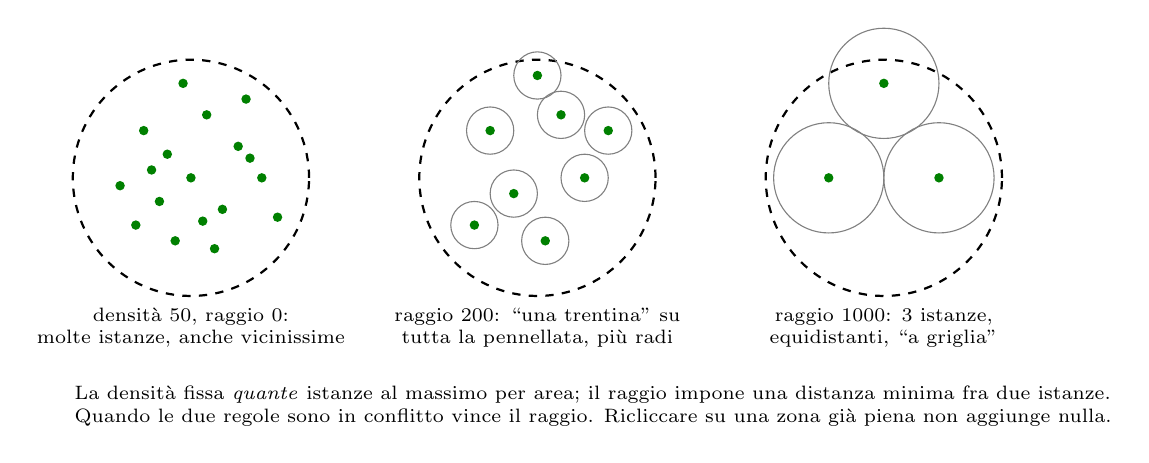
\begin{tikzpicture}[font=\scriptsize, x=1cm, y=1cm]
  % pannello 1: raggio 0
  \draw[thick, dashed] (1.6,1.6) circle (1.5);
  \foreach \p in {(1.0,2.2),(1.3,1.9),(1.8,2.4),(2.2,2.0),(0.7,1.5),(1.2,1.3),(1.6,1.6),(2.0,1.2),(2.5,1.6),(1.4,0.8),(1.9,0.7),(0.9,1.0),(2.3,2.6),(1.5,2.8),(2.7,1.1),(1.1,1.7),(1.75,1.05),(2.35,1.85)}
    {\fill[green!50!black] \p circle (0.06);}
  \node[align=center] at (1.6,-0.3) {densità 50, raggio 0:\\molte istanze, anche vicinissime};
  % pannello 2: raggio medio
  \begin{scope}[xshift=4.4cm]
    \draw[thick, dashed] (1.6,1.6) circle (1.5);
    \foreach \p in {(1.0,2.2),(1.9,2.4),(1.3,1.4),(2.2,1.6),(0.8,1.0),(1.7,0.8),(2.5,2.2),(1.6,2.9)}
      {\fill[green!50!black] \p circle (0.06); \draw[gray] \p circle (0.3);}
    \node[align=center] at (1.6,-0.3) {raggio 200: ``una trentina'' su\\tutta la pennellata, più radi};
  \end{scope}
  % pannello 3: raggio grande
  \begin{scope}[xshift=8.8cm]
    \draw[thick, dashed] (1.6,1.6) circle (1.5);
    \foreach \p in {(0.9,1.6),(2.3,1.6),(1.6,2.8)}
      {\fill[green!50!black] \p circle (0.06); \draw[gray] \p circle (0.7);}
    \node[align=center] at (1.6,-0.3) {raggio 1000: 3 istanze,\\equidistanti, ``a griglia''};
  \end{scope}
  \node[align=left, anchor=west] at (0,-1.3) {La densità fissa \emph{quante} istanze al massimo per area; il raggio impone una distanza minima fra due istanze.\\Quando le due regole sono in conflitto vince il raggio. Ricliccare su una zona già piena non aggiunge nulla.};
\end{tikzpicture}
\caption{Densità e raggio nel Foliage Mode, con i numeri delle prove della lezione. Il
cerchio tratteggiato è il pennello; i cerchi grigi attorno alle istanze rappresentano il
raggio minimo. Ricostruzione schematica: le posizioni dei punti sono indicative.}
\label{ue15:fig:raggio}
\end{figure}

\paragraph{Approfondimento: come piazza il pennello.} Il comportamento visto a lezione è
coerente con il modo in cui il Foliage Mode lavora. A ogni pennellata calcola quante istanze
dovrebbero esserci nell'area del pennello in base a \emph{Density} (istanze per
1000$\times$1000 unità, cioè per 10$\times$10 metri) e alla \emph{Paint Density}; conta quelle
già presenti dello stesso tipo e aggiunge solo le mancanti, scartando ogni posizione
candidata che cada entro il \emph{Radius} di un'istanza esistente. Da qui le tre cose
osservate: ricliccare non aggiunge nulla quando la zona è ``piena''; togliendo il raggio si
riempiono i buchi che il raggio aveva scartato; con un raggio grande la densità teorica non
si raggiunge mai, e le istanze si dispongono a distanza quasi costante. Il raggio è anche il
modo più semplice per evitare alberi compenetrati, il problema che Totten chiama
\emph{casualità percepita} (si veda l'approfondimento della
sezione~\ref{ue15:sec:selezione}). Funzionamento generale dell'engine.

% ---------------------------------------------------------------------
\section{Le altre impostazioni: pendenza, altezza, mobilità, collisioni}
\label{ue15:sec:altre}

\paragraph{Align to Normal e Align Max Angle.} \textbf{Align to Normal} decide se le istanze
``sono allineate alla normal su cui sono applicate''. \textbf{Align Max Angle} è ``quanto si
inclinano per aggiustarsi alla singola pendenza'' (il docente in un primo momento lo confonde
con il parametro successivo e si corregge: ``no, aspetta, mi sa che\dots'').

\paragraph{Ground Slope Angle.} È ``il range in cui il foliage verrà piazzato'': l'angolo
minimo e massimo della superficie su cui un'istanza può comparire. Il docente dipinge l'erba
su un pendio (dopo un momento di confusione: ``stavo modificando ancora le cose dell'albero
invece era l'erba che andava modificata; ci ho cliccato sopra, pensavo di averla selezionata e
invece non era selezionata'', ``è il tipo di cose che vi capiterà sicuramente ogni tanto''). Con
l'intervallo di default, fino a 180, l'erba va ``anche sulla parete rocciosa''. ``Poi sta a voi
decidere se volete che il foliage venga piazzato anche lì oppure no.'' Con un massimo di
\textbf{45} gradi, l'erba compare ``soltanto nelle parti della slope che erano sotto i 47
gradi'' (il docente dice 47 avendo impostato 45: con ogni probabilità è un lapsus), e si
ammucchia nei punti meno ripidi. Abbassando ancora, ``neanche su questa cunetta è stata
messa, perché l'angolazione è troppo alta''. Un uso: mettere attorno alla base del
``montarozzo'' dell'erba a mano, ``per far vedere che un minimo c'è stata un'espansione
erbosa'', senza che salga sulle pareti; ``anche troppo preciso, devo dire''. Il docente lo
rimette a 45 (figura~\ref{ue15:fig:slope}).

\begin{figure}[htbp]
\centering
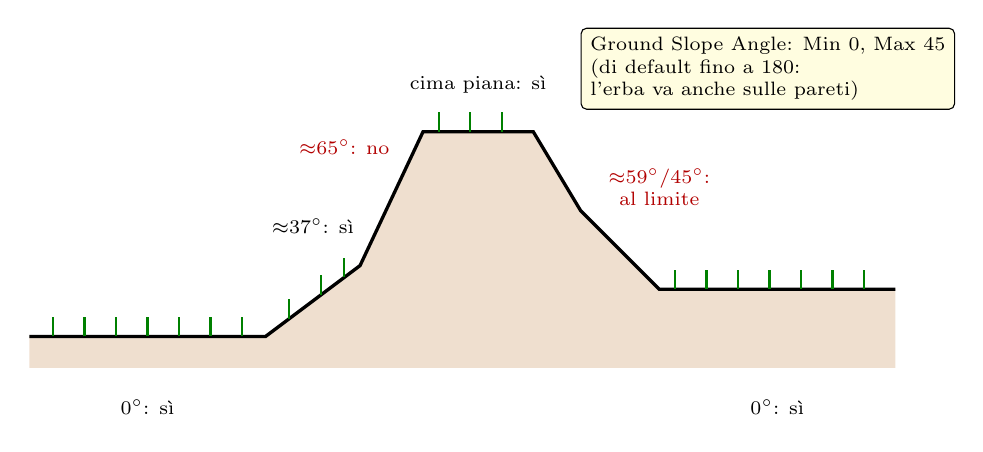
\begin{tikzpicture}[font=\scriptsize, x=1cm, y=1cm]
  \fill[brown!25] (0,0) -- (3,0) -- (4.2,0.9) -- (5.0,2.6) -- (6.4,2.6) -- (7.0,1.6) -- (8.0,0.6) -- (11,0.6) -- (11,-0.4) -- (0,-0.4) -- cycle;
  \draw[very thick] (0,0) -- (3,0) -- (4.2,0.9) -- (5.0,2.6) -- (6.4,2.6) -- (7.0,1.6) -- (8.0,0.6) -- (11,0.6);
  % erba
  \foreach \x in {0.3,0.7,...,2.9} {\draw[green!50!black, thick] (\x,0) -- (\x,0.25);}
  \foreach \x in {3.3,3.7,4.0} {\draw[green!50!black, thick] (\x,{0.75*(\x-3)}) -- (\x,{0.75*(\x-3)+0.25});}
  \foreach \x in {5.2,5.6,...,6.3} {\draw[green!50!black, thick] (\x,2.6) -- (\x,2.85);}
  \foreach \x in {8.2,8.6,...,10.9} {\draw[green!50!black, thick] (\x,0.6) -- (\x,0.85);}
  \node[align=center] at (1.5,-0.9) {0$^\circ$: sì};
  \node[align=center] at (3.6,1.4) {$\approx$37$^\circ$: sì};
  \node[align=center, red!70!black] at (4.0,2.4) {$\approx$65$^\circ$: no};
  \node[align=center] at (5.7,3.2) {cima piana: sì};
  \node[align=center, red!70!black] at (8.0,1.9) {$\approx$59$^\circ$/45$^\circ$:\\al limite};
  \node[align=center] at (9.5,-0.9) {0$^\circ$: sì};
  \node[align=left, anchor=west, draw, rounded corners=2pt, fill=yellow!12] at (7.0,3.4) {Ground Slope Angle: Min 0, Max 45\\(di default fino a 180:\\l'erba va anche sulle pareti)};
\end{tikzpicture}
\caption{Il Ground Slope Angle di un foliage type. Con un massimo di 45 gradi il pennello
piazza istanze solo dove la superficie è inclinata meno di 45 gradi rispetto all'orizzontale;
le pareti restano spoglie. Gli angoli indicati sono esempi. Ricostruzione schematica.}
\label{ue15:fig:slope}
\end{figure}

\paragraph{Height.} Il range d'altezza in cui il foliage può essere piazzato. Di default va
da meno a più infinito (``da meno a più''); con \textbf{0 -- 10}, ``appena andiamo sopra i 10
d'altezza, lui smette di piazzarla''.

\paragraph{Mobility.} Come per le luci: \textbf{Static}, ``più veloci da renderizzare'', che
``funzionano col baking'', o \textbf{Movable}, ``completamente dinamiche'', con le luci che
``reagiscono in tempo reale'', ``ma è più lento da gestire''.

\paragraph{Cull Distance.} ``La distanza massima da cui non smettono di essere renderizzate.''
Allontanandosi, ``tutto il resto del foliage è sparito'', quello del materiale, ``ma questo è
rimasto, perché c'è zero di cull distance'': ``non ha massimo e minimo, esiste e basta, non viene
tagliato, è sempre renderizzato''. ``Gestitelo sulla base della grandezza della vostra scena.''

\paragraph{Le ombre e il dressing.} \emph{Cast Shadow}, ombre dinamiche e statiche,
\emph{Affect Dynamic Lighting}: ``tutti i check che potete gestirvi per la resa estetica con
la luce''. L'erba del pacchetto ``è fatta apposta per non castare ombre''. Il foliage si può
dipingere anche \emph{sopra} le mesh: il docente mette dell'erba sopra una struttura della
base, e immagina ``un mondo post apocalittico con una pompa di benzina abbandonata'' (``non so
perché mi ha fatto pensare alla pompa di benzina''), con l'erba che ci cresce sopra e ``dei
\emph{vine} che scendono giù'' (delle liane, dei rampicanti).

\paragraph{Collision Presets.} ``E poi abbiamo i preset delle collisioni.'' La frase del docente
è ambigua (``di default tutto il foliage è impostato a una collisione, che nel caso dell'erba
ci fa anche comodo, perché noi non vogliamo che ci sia l'erba e poi ci inciampiamo sopra''):
il senso è che \emph{per l'erba} si vuole che non ci siano collisioni. ``Quando andiamo a
mettere gli alberi, però, dobbiamo assicurarci che lì sia tutto funzionale, che le collisioni
ci siano, perché altrimenti possiamo passarci attraverso.''

\paragraph{L'ingresso della base.} Prima degli alberi il docente sistema l'erba davanti alla
base: ``il nostro personaggio uscirà da lì e si trova prima l'erbetta che va a gradiente, poi
c'è il folto''.

\paragraph{Approfondimento: le impostazioni del foliage type.} Qualche precisazione sui
parametri visti. \emph{Ground Slope Angle} confronta la normale della superficie con la
verticale, come il World Aligned Blend dell'automaterial: le due cose si possono far
coincidere, così che il foliage manuale non finisca dove il materiale mette la roccia.
\emph{Height} usa la quota assoluta del mondo in centimetri, quindi ``0 -- 10'' è una fascia di
dieci centimetri sopra lo zero del mondo, utile per esempio per non piantare canne sopra il
livello dell'acqua. \emph{Cull Distance} ha un minimo e un massimo: fra i due le istanze
sfumano, e con entrambi a 0 il culling per distanza è disattivato, come visto. I
\emph{Collision Presets} del foliage type (\emph{Body Instance}) decidono come le istanze
\emph{rispondono} alle collisioni; perché ci sia una collisione, però, la mesh deve averne una
(la sezione successiva lo mostra). Romero e Sewell descrivono nel capitolo 14 (``Math and
Trace Nodes'') la tabella delle \emph{Collision Responses}: ogni oggetto ha un \emph{Object
Type} e una risposta (\emph{Ignore}, \emph{Overlap} o \emph{Block}) per ogni canale, con dei
preset come \emph{BlockAll}, \emph{OverlapAllDynamic} e \emph{Pawn}, oppure
\emph{Custom\ldots}; nel capitolo 5 impostano \emph{BlockAllDynamic} su un oggetto
interattivo. Le stesse regole valgono per le istanze del foliage.

% ---------------------------------------------------------------------
\section{Gli alberi e le collisioni}
\label{ue15:sec:alberi}

\paragraph{Le impostazioni dell'albero.} ``Togliamo l'erba, perché sennò dipingiamo anche
l'erba insieme agli alberi.'' Le impostazioni del pacchetto: \textbf{Density 1}, ``abbastanza
sparsi'', raggio 0: ``ci può stare''. Il docente ne mette una fila all'ingresso, ``una piccola
radura''. Gli alberi sono di taglie diverse (\textbf{Scale} da 1 a 3: ``con l'albero funziona
meglio, dà un'idea migliore''; c'è l'albero ``di base'' e ``l'albero grosso'') e ruotati in
maniera diversa: lo Z Offset è 0, ma c'è il \textbf{Random Yaw}, ``una rotazione randomica
sull'asse verticale''. Togliendolo, ``gli alberi vanno tutti nella stessa direzione, sono tutti
curvi in quella direzione, verso sinistra''; rimettendolo, ``iniziano a ruotare''. (Un albero
``si è rifiutato di essere cancellato''.)

\paragraph{Alberi dalle pareti.} Lasciando il Ground Slope Angle ampio e Align to Normal
attivo, si possono piantare alberi su una parete: ``alberi che escono dalle pareti, non so
perché dovreste volerlo fare, ma lo potete fare''. Per esempio ``un percorso di alberi tutto
attaccato sul lato della parete, che potete utilizzare come percorso per un platform''.
Togliendo Align to Normal ``ve li spawna dritti''. Con gli alberi l'allineamento ``non funziona
granché bene'', ``ma per esempio con dei cespugli o dei funghi parassiti'' sì.

\paragraph{La collisione strana.} Le collisioni dell'albero sono \textbf{Block All}. ``Col
nostro robottino andiamo all'avventura'': ``siamo alti quanto l'erba'' (bisognerà abbassarla).
In Play si riesce a passare dentro gli alberi, almeno in parte: ``hanno una strana
collisione''. Prima di guardare, il docente chiarisce ``una grossa cosa'' sulle collisioni:
``questo parametro non determina se l'oggetto avrà collisioni o meno; determina se le
collisioni dell'oggetto sono attive o meno, e per cosa sono attive''. La prova: Block All
sull'\textbf{erba}. ``Sono positivamente sicuro che potremo comunque camminare dentro l'erba'':
ed è così (``se dovessimo esplorare un open world del genere, il nostro personaggio dovrebbe
muoversi più veloce di così''). Il motivo è nella static mesh di base: nello Static Mesh
Editor, con \textbf{Show Simple Collision}, ``non ci sono simple collision, quindi non c'è
nulla da attivare''. ``Vi capiterà di mettere degli asset in scena, iniziare a giocare e
passarci attraverso, perché magari quegli asset sono stati importati o esportati senza le
collisioni''; e anche impostando ``le collisioni che bloccano tutto, o che bloccano solo i
proiettili'', ``lui comunque non può bloccare, perché non c'è nulla da bloccare''.

\paragraph{L'albero, dentro.} Aprendo la mesh dell'albero: ``ah, geniale. L'hanno messa dalla
parte sbagliata.'' Le forme della collisione semplice (``diversi pezzi'') sono ruotate rispetto
al tronco, ``credo che l'abbiano importato proprio con la collisione sbagliata''. Si possono
selezionare tutte e ruotare ``dalla parte corretta''; ``anche se sono proprio strane'',
sbagliate anche nelle proporzioni. Tre strade:
\begin{enumerate}
  \item \textbf{ruotare} le forme esistenti, come fa il docente (``tanto il nostro giocatore
        non andrà mai a collidere lassù, a meno che non vogliamo che lo faccia'');
  \item \textbf{eliminare} le simple collision e scegliere \textbf{Use Complex Collision As
        Simple}: la collisione prende ``esattamente i poligoni dell'albero''. ``Chiaramente
        questa cosa è pesante, però vi risolve il problema di dover fare le collisioni a
        mano'';
  \item \textbf{rifarle} a mano con forme semplici: ``vi basterebbe prendere un cilindro,
        metterlo in diagonale, e qui sopra metterci un piano circolare''. Il docente aggiunge
        una \textbf{capsula}, la fa più piccola e più stretta, la ruota lungo il tronco, e
        sopra una \textbf{box piatta}, ``in modo che il giocatore possa salire sulla cima
        dell'albero e rimanerci sopra'' (figura~\ref{ue15:fig:collisione}).
\end{enumerate}
Se si vuole che il personaggio salti da un albero all'altro o percorra la parete passando sui
tronchi, ``non potete fare questa cosa'' con la collisione originale: ``dovete togliere queste
collisioni e rifarle''.

\begin{figure}[htbp]
\centering
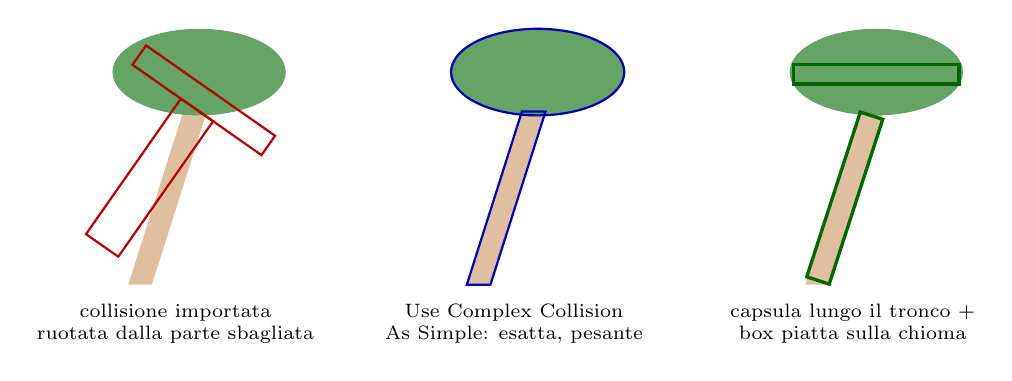
\begin{tikzpicture}[font=\scriptsize, x=1cm, y=1cm]
  % albero originale
  \begin{scope}
    \fill[brown!50] (0.9,0) -- (1.2,0) -- (1.9,2.2) -- (1.6,2.2) -- cycle;
    \fill[green!40!black!60] (1.8,2.7) ellipse (1.1 and 0.55);
    \draw[red!70!black, thick, rotate around={-35:(1.2,1.4)}] (0.95,0.3) rectangle (1.45,2.4);
    \draw[red!70!black, thick, rotate around={-35:(1.2,1.4)}] (0.2,2.4) rectangle (2.2,2.7);
    \node[align=center] at (1.5,-0.5) {collisione importata\\ruotata dalla parte sbagliata};
  \end{scope}
  % complex as simple
  \begin{scope}[xshift=4.3cm]
    \fill[brown!50] (0.9,0) -- (1.2,0) -- (1.9,2.2) -- (1.6,2.2) -- cycle;
    \fill[green!40!black!60] (1.8,2.7) ellipse (1.1 and 0.55);
    \draw[blue!70!black, thick] (0.9,0) -- (1.2,0) -- (1.9,2.2) -- (1.6,2.2) -- cycle;
    \draw[blue!70!black, thick] (1.8,2.7) ellipse (1.1 and 0.55);
    \node[align=center] at (1.5,-0.5) {Use Complex Collision\\As Simple: esatta, pesante};
  \end{scope}
  % capsula + box
  \begin{scope}[xshift=8.6cm]
    \fill[brown!50] (0.9,0) -- (1.2,0) -- (1.9,2.2) -- (1.6,2.2) -- cycle;
    \fill[green!40!black!60] (1.8,2.7) ellipse (1.1 and 0.55);
    \draw[green!40!black, very thick, rotate around={-18:(1.4,1.1)}] (1.25,0.0) rectangle (1.55,2.2);
    \draw[green!40!black, very thick] (0.75,2.55) rectangle (2.85,2.8);
    \node[align=center] at (1.5,-0.5) {capsula lungo il tronco +\\box piatta sulla chioma};
  \end{scope}
\end{tikzpicture}
\caption{Tre modi di sistemare la collisione dell'albero di StackOBot visti a lezione:
ruotare le forme importate male, usare la geometria della mesh come collisione, oppure
rifare la collisione con una capsula (qui disegnata come un rettangolo inclinato) e una box
piatta su cui il giocatore può stare in piedi. Ricostruzione schematica.}
\label{ue15:fig:collisione}
\end{figure}

\paragraph{La domanda sulle collisioni a senso unico.} Uno studente ha una domanda ``fuori
tema'': ``le collisioni che funzionano da un solo lato?'' Gli è venuto in mente un gioco (``PIC''
nella trascrizione: con ogni probabilità \emph{PEAK}, il gioco cooperativo di arrampicata, ma
il nome non è certo) in cui ``puoi salire sugli alberi e puoi attraversare le foglie da sotto,
ma non puoi attraversarle da sopra''. Il docente non ci ha mai pensato: ``probabilmente dipende
dal modo in cui è codificato quel tipo di interazione''. ``Gli dici che se stai andando in una
direzione non deve contare quella collisione, se stai andando nell'altra deve contarla.
Penso, non lo so, a naso direi che è questo.'' Non ha giocato il gioco.

\paragraph{No Collision sovrascrive.} Rimesso tutto com'era, con le collisioni girate ``dalla
parte giusta'', il docente imposta \textbf{No Collision} nel foliage type dell'albero: ``lui
sovrascrive il fatto che ha delle collisioni''. In Play ci si passa attraverso, ``perché l'asset
del foliage non ha collisioni''. Con \textbf{Custom} si sceglie che cosa bloccano: ``se bloccano
la camera, se bloccano i proiettili, se bloccano il pawn''. ``Di base, il Block All andrà
bene.''

\paragraph{Approfondimento: collisione semplice, complessa e a senso unico.} Una static mesh
ha due rappresentazioni di collisione. La \emph{simple collision} è fatta di primitive
(box, sfere, capsule, convessi) ed è quella usata dalla fisica e dal movimento del
personaggio: è economica, ma va costruita (nello Static Mesh Editor, menu
\emph{Collision}: \emph{Add Box}, \emph{Add Capsule}, \emph{Auto Convex Collision}\dots)
o importata dal programma di modellazione. La \emph{complex collision} è la mesh stessa,
triangolo per triangolo, usata di solito solo per le tracce precise. \emph{Collision
Complexity: Use Complex Collision As Simple} fa usare la seconda anche per la fisica: comoda,
ma costosa su mesh dense e, per i corpi simulati, non utilizzabile. Le collisioni ``a senso
unico'' delle piattaforme attraversabili da sotto non sono una proprietà della collisione
in Unreal: si ottengono via codice, per esempio con un volume sotto la piattaforma che, quando
il personaggio sale, gli fa ignorare il canale della piattaforma (\emph{Ignore}) e lo
ripristina quando il personaggio è sopra, oppure controllando la velocità verticale; è
proprio la risposta ``a naso'' del docente. Le risposte \emph{Ignore}/\emph{Overlap}/\emph{Block}
per canale sono quelle della tabella del capitolo 14 di Romero e Sewell; il resto è
funzionamento generale dell'engine.

% ---------------------------------------------------------------------
\section{Selezionare, rifinire e il foliage non naturale}
\label{ue15:sec:selezione}

\paragraph{Il cespuglio a mano.} ``Lo stesso con gli altri oggetti.'' Il cespuglio del
pacchetto spawna poco; è ``un tipo di asset che io, piuttosto che metterlo così, farei
\textbf{single} e andrei a posizionare a mano'': ``voglio che queste cose stiano molto
ammucchiate vicino agli alberi''. Le dimensioni sono comunque casuali, ``forse troppo varie
per i miei gusti''. Allo stesso modo si fa ``un percorso alberato'', con alberi a destra e a
sinistra, che ``fa comunque parte del foliage'' e si integra con il resto.

\paragraph{Gli strumenti di selezione.}
\begin{itemize}
  \item \textbf{Select}: si prende ``il singolo pezzo di foliage'' e lo si sposta (``no, no,
        quest'albero non deve stare proprio lì, deve stare qui''), ``un po' tipo selection mode,
        ma con tutti gli asset che rimangono all'interno del foliage''. Tornando in Selection
        Mode e cliccando, invece, si seleziona tutto il foliage actor. (Il docente trova
        nell'Outliner anche delle istanze che non si aspettava, ``saranno delle cose che
        c'erano prima'', e non approfondisce.)
  \item \textbf{Select All} e \textbf{Deselect}: tutte le istanze dei tipi attivi, da
        muovere insieme.
  \item \textbf{Select Invalid}: ``mi porta automaticamente alle instance che sono invalide,
        quindi quelle che vanno modificate''.
  \item \textbf{Lasso}: ``funziona un po' tipo Photoshop'': invece di cliccare, si evidenzia
        una zona. Vale solo per i tipi spuntati: ``qui ci sono sempre attivi soltanto gli
        alberi, quindi se voglio fare questa cosa devo prendere anche questi''.
  \item \textbf{Remove}: ``questi alberi qua non mi piacciono'': elimina tutto ciò che è stato
        evidenziato.
  \item un ultimo strumento, ``stessa cosa con i raise, però è un discorso un po' diverso, poi
        modifica piano piano'': il nome non è ricostruibile con certezza (con ogni probabilità
        \emph{Reapply}, che riapplica le impostazioni del foliage type alle istanze già
        dipinte).
\end{itemize}

\paragraph{Non deve essere naturale.} ``È tendenzialmente uno strumento che utilizzate
principalmente per motivi estetici.'' E ``non deve essere necessariamente naturale'': si può
usare ``con ogni mesh che voglio''. ``Se io voglio riempire la scena di robottini, lo posso
fare''; una scena in metropolitana con il pavimento pieno di ``cartacce, plastiche, cose
varie''. ``È un po' un pennello con cui piazzare rapidamente tutta una serie di oggetti.''

\paragraph{Le rocce sotto lo zero.} Le rocce dipinte ``appena si avvicinano allo zero
impazziscono; invece sopra sono perfette''. Consiglio: ``mettete il piano di base leggermente
più alto dello zero''. Spostando una roccia, il materiale cambia: ``cambia sulla base
dell'altezza''; ruotandola, ``così diventa una parete rocciosa''. ``È un po' strano che abbiano
scelto di fare un materiale dinamico così per un oggetto standard.'' Aprendo il materiale
(``più complesso di quello che pensavo''), il docente legge nomi come \emph{Virtual
Texture}, \emph{World Position} e una ``variation'' (la trascrizione dice ``part time, drop
variation'', non ricostruibile): ``hanno provato a fare una roba carina'' per avere un
materiale dinamico, ``tipo il \textbf{vertex painting}'', e per ``blendare la mesh con
l'oggetto del landscape'' quando si dipinge il materiale del landscape. Ma ``volendo, potete
fare anche letteralmente solo una texture di roccia'' con le sue mappe, ``e avete comunque una
roccia''.

\paragraph{Approfondimento: la casualità percepita.} Il Foliage Mode rende facilissimo
spargere oggetti a caso, ed è proprio il rischio che Totten descrive nel capitolo 8
(``Possibility Spaces and Worldbuilding''): in natura alberi, rocce e scogliere si dispongono
nel tempo in modi non pianificati, e i designer alle prime armi piazzano alberi, rocce ``e
perfino edifici'' a caso sulla mappa, ``ignari dell'importanza della loro posizione''; il
risultato è una \emph{casualità percepita} che non dice nulla al giocatore. ``Dirigere lo
sguardo verso elementi scenici piazzati con cura'' è il modo in cui il giocatore capisce il
mondo. In pratica: il pennello per la massa (l'erba, il bosco di sfondo), lo \emph{Single
Instance Mode} e il \emph{Select} per gli elementi che contano (l'albero isolato che fa da
landmark, i cespugli che incorniciano un passaggio), che è esattamente il modo di lavorare del
docente con i cespugli. Nel capitolo 3 (``Basic Gamespaces'') Totten aggiunge che un cambio
nel tipo di vegetazione segnala il passaggio a una zona nuova, come un cambio di texture sul
terreno. Sul materiale delle rocce: un materiale che campiona texture in world space
(\emph{world aligned}) cambia aspetto quando l'oggetto si sposta o ruota, perché la texture
resta ferma nel mondo mentre la mesh si muove; e un calcolo basato sulla quota assoluta (per
esempio per sfumare la base nella sabbia o nell'umidità) produce effetti strani sotto lo
zero, se chi l'ha fatto ha supposto che il terreno stia sopra. Funzionamento generale
dell'engine; il grafo del materiale non è stato verificato nel capitolo.

% ---------------------------------------------------------------------
\section{La domanda sui mondi procedurali}
\label{ue15:sec:procedurale}

\paragraph{Landscape o mesh?} ``Ci sono domande?'' Uno studente: ``i mondi che si generano
automaticamente usano il landscape o le mesh?'' ``Tipo le robe procedurali? Tendenzialmente
dipende.'' ``È più comodo farlo con le mesh, perché puoi farti un \textbf{array} di oggetti e
puoi piazzarli secondo dei criteri che hai scelto tu.'' Ma ``l'ultima volta che ho lavorato
con qualcosa di procedurale era un sacco di tempo fa'', e magari ci sono ``nuovi nodi'' o
``feature che Unreal ha inserito'' che il docente non conosce. Il consiglio: cercare sullo store
``qualche pacchetto che parla di asset procedurali, non modulari, proprio procedurali, che ha
dei sistemi di proceduralizzazione'', e ``ti studi un po' loro come le fanno''. ``Fab, intendi,
giusto?'' ``Sì, su Fab. Ai miei tempi non si chiamava Fab, mi sento vecchio.''

\paragraph{Lo strumento che non si trova.} Parlando di procedurale, il docente ricorda ``un
tool che io non ho mai usato, che dovrebbe essere relativamente nuovo'': ``una specie di box
all'interno della quale possono essere impostati dei parametri, e spostando questa box e
ingrandendola, lui va a piazzare quel tipo di foliage nel volume che c'è all'interno''. Lo
cerca fra i tipi di asset del menu \emph{Foliage} (c'è lo \emph{Static Mesh Foliage}, ``questo
qui è letteralmente il nuovo, ma non è quello che voglio''), non lo trova, e ipotizza che
fosse ``un plugin''. ``Me lo devo vedere meglio.''

\paragraph{Sprite e flipbook.} Nello stesso menu ``vi potete vedere tutti i tipi di asset che
possono essere creati'', anche gli \textbf{sprite} e i \textbf{flipbook}: ``carini se volete
fare, che ne so, un menu animato''. ``Visto che avete fatto la roba col menu, con un flipbook
potete andare a fare l'animazione del menu.''

\paragraph{Approfondimento: generazione procedurale in Unreal.} Lo strumento descritto dal
docente corrisponde con ogni probabilità a uno di due sistemi, ed entrambi si attivano da
plugin. Il primo è il \emph{Procedural Foliage Spawner} con il suo \emph{Procedural Foliage
Volume}: si definisce quali foliage type crescono, con quali regole di competizione e di
età, e si fa ``simulare'' la crescita dentro il volume (è una funzione sperimentale,
\emph{Procedural Foliage}, da abilitare nelle impostazioni dell'editor). Il secondo, più
recente e oggi il sistema di riferimento, è il framework \emph{PCG} (\emph{Procedural
Content Generation}), con il \emph{PCG Volume} e un grafo a nodi che campiona superfici,
filtra i punti per pendenza o altezza e vi genera mesh: il plugin si chiama
\emph{Procedural Content Generation Framework}. La risposta del docente sulle mesh resta
valida: anche il PCG, alla fine, produce istanze di static mesh. Romero e Sewell, nel
capitolo 19 (``Procedural Generation''), definiscono la generazione procedurale come ``un
metodo per creare il contenuto del livello usando script invece che a mano'', utile per
evitare compiti ripetitivi; la costruiscono con il \emph{Construction Script}, un
\emph{Instanced Static Mesh Component} e dei cicli \emph{For Loop} che dispongono righe di
istanze, e poi con le \emph{Blueprint Spline} per piazzare actor lungo un percorso. Gli
sprite e i flipbook appartengono a \emph{Paper2D}, il sistema 2D dell'engine: un flipbook è
una sequenza di sprite riprodotta a una certa velocità. Fab è lo store di Epic che dal 2024
ha sostituito l'Unreal Engine Marketplace, quello usato nel capitolo 9 del libro per
importare l'\emph{Animation Starter Pack}.

% ---------------------------------------------------------------------
\section{Il Niagara e il Post Process Volume}
\label{ue15:sec:postprocess}

``Come ho detto, ci abbiamo una decina di minuti.'' In quella decina di minuti si potrebbe
``buttare un occhio'' sul post process, ``visto che ci siamo''.

\paragraph{Un'occhiata al Niagara.} Prima, ``al volo'', il Niagara: ``è proprio un editor a
parte''. Creando un \textbf{Niagara System} si sceglie fra ``tutte le varie forme, modi, colori,
possibilità'' dei \emph{preset}; il docente prende una \textbf{Fountain}, ``la base della
cosa''. Dentro c'è ``tutto un sistema così, con la timeline, con degli \textbf{emitter}, tutte
cose''. ``È una roba un po' complicata, magari ce la vediamo alla prossima lezione se
riusciamo.''

\paragraph{Dove si trova il post process.} Dal \textbf{Place Actors}, nella categoria
\textbf{Volumes}, ``tra le varie cose'' (``insieme a tutta una serie di altre cose molto, molto
carine'') c'è il \textbf{Post Process Volume}: ``il nostro quadratone''.

\paragraph{Che cos'è.} ``È un volume all'interno del quale voi andate ad applicare delle
modifiche alla lente della telecamera, fondamentalmente.'' ``Voi andate a modificare il modo in
cui le cose appaiono, non il modo in cui le cose sono.'' Le stesse ``lenti'' esistono anche su
una \textbf{Camera Actor}: nei suoi Details, nella sezione \emph{Post Process}, ``abbiamo
diverse lenti che possiamo andare a modificare'', e queste modifiche ``si applicano solo alla
singola telecamera''. Il volume invece applica gli effetti \emph{al suo interno}.

\paragraph{Le transizioni.} ``Vi siete mai chiesti come fanno a fare quegli effetti per cui
quando entri o esci da una casa il bloom della luce è particolarmente forte e poi si attenua?
O com'è possibile che la luce fuori era molto forte, io entro dentro una grotta e piano piano
la luce diventa più tenue e cambia colore?'' ``È perché il post process ha degli effetti di
transizione fra l'interno e l'esterno.'' Si possono piazzare più Post Process Volume con
effetti diversi, e passando dall'uno all'altro cambia ``il modo in cui la mia telecamera va a
gestire le cose''.

\paragraph{I volumi annidati.} Si può anche mettere un post process dentro un altro, ``una roba
complicata che vi sconsiglierei di fare'': il volume interno ``calcola tutto quello che lui
deve calcolare e in più ci applica anche quello'' dell'esterno. L'esempio: il volume interno
rende la scena gialla (\emph{color correction}), quello esterno blu; stando nell'interno ``vediamo
tutto verde, perché lui somma la color correction dei due post process''. ``Per cui diventa molto
complicato capire cosa vogliamo fare.'' (Figura~\ref{ue15:fig:postprocess}.)

\paragraph{Un solo volume per tutto: Infinite Extent.} ``Se voglio un unico post process che
determina il modo in cui la scena viene vista, devo renderlo incredibilmente grande?'' No:
nei Details del volume (``le stesse lenti che aveva il camera actor, con qualche opzione in
più'') si cerca \emph{infinite} e si trova \textbf{Infinite Extent (Unbound)}: ``quando questa
casella viene spuntata, il volume copre tutto il mondo, non solo l'area all'interno'', e i
cambiamenti ``vengono visti allo stesso modo in tutta la zona''. Per ora la si toglie.

\paragraph{Le lenti, per la prossima volta.} ``Non so quanto senso abbia iniziare a parlare
delle lenti: ci abbiamo 5 minuti, e ogni lente ha un sacco di parametri.'' Due accenni: il
\textbf{Bloom}, ``abbastanza semplice'', ``quello che serve per i god shaft'' di cui si parlava
prima; e la \textbf{Chromatic Aberration}: ``occhio, che fa male agli occhi''. Il resto alla
prossima lezione.

\begin{figure}[htbp]
\centering
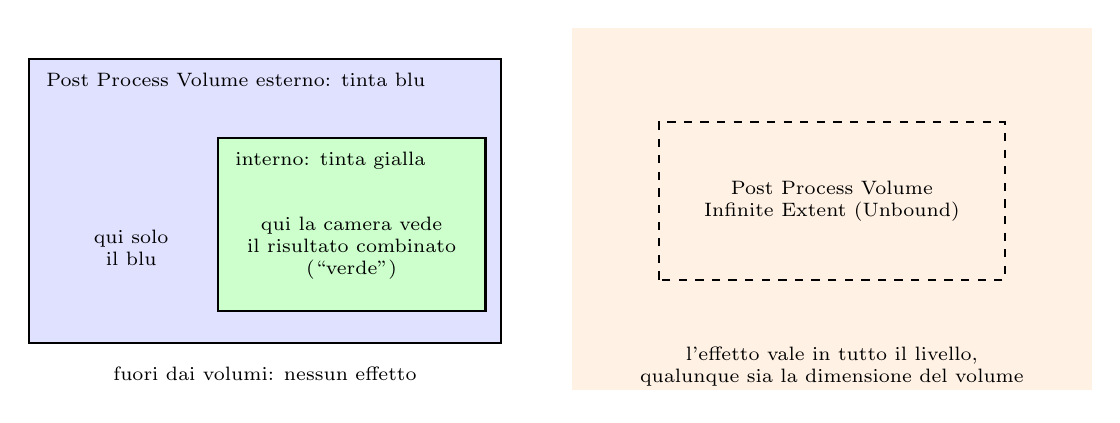
\begin{tikzpicture}[font=\scriptsize, x=1cm, y=1cm]
  \draw[thick, fill=blue!12] (0,0) rectangle (6,3.6);
  \node[anchor=north west] at (0.1,3.55) {Post Process Volume esterno: tinta blu};
  \draw[thick, fill=green!20] (2.4,0.4) rectangle (5.8,2.6);
  \node[anchor=north west, align=left] at (2.5,2.55) {interno: tinta gialla};
  \node[align=center] at (4.1,1.2) {qui la camera vede\\il risultato combinato\\(``verde'')};
  \node[align=center] at (1.3,1.2) {qui solo\\il blu};
  \node[align=center] at (3,-0.4) {fuori dai volumi: nessun effetto};
  % unbound
  \begin{scope}[xshift=7.2cm]
    \fill[orange!10] (-0.3,-0.6) rectangle (6.3,4.0);
    \draw[thick, dashed] (0.8,0.8) rectangle (5.2,2.8);
    \node[align=center] at (3,1.8) {Post Process Volume\\Infinite Extent (Unbound)};
    \node[align=center] at (3,-0.3) {l'effetto vale in tutto il livello,\\qualunque sia la dimensione del volume};
  \end{scope}
\end{tikzpicture}
\caption{A sinistra, due Post Process Volume annidati: dentro il volume interno la camera
riceve l'effetto di entrambi, come nell'esempio del docente (giallo e blu che danno verde). A
destra, un volume con \emph{Infinite Extent (Unbound)}, che vale per tutto il livello.
Ricostruzione schematica.}
\label{ue15:fig:postprocess}
\end{figure}

\paragraph{Approfondimento: come si combinano i post process.} Il comportamento dei volumi
sovrapposti è un po' più ordinato della ``somma'' descritta a lezione. Ogni Post Process
Volume ha una \emph{Priority}, un \emph{Blend Weight} (da 0 a 1) e un \emph{Blend Radius}, la
distanza dal bordo entro cui l'effetto sfuma: è il Blend Radius che produce le transizioni
graduali fra esterno e grotta. Ogni volume modifica solo le proprietà la cui casella è
spuntata; quando la camera è dentro più volumi, Unreal li applica in ordine di priorità, e
per ogni proprietà il valore del volume a priorità più alta si \emph{mescola} con quello già
calcolato secondo il suo Blend Weight (con peso 1 lo sostituisce). Se due volumi cambiano
proprietà diverse, si vedono entrambe le modifiche; se cambiano la stessa con peso minore di
1, si ottiene una via di mezzo: in questo senso le due tinte possono dare un colore
combinato. Il consiglio del docente resta buono: pochi volumi, priorità esplicite, e di solito
un volume \emph{Unbound} a priorità bassa per l'aspetto generale del livello più volumi locali
per le zone speciali. Le impostazioni della Camera Actor (e del \emph{Camera Component} del
personaggio) si combinano con quelle dei volumi, con un proprio peso. Romero e Sewell, nel
capitolo 9 (``Building Smart Enemies with Artificial Intelligence''), allargando l'area di
gioco ricordano che il \emph{PostProcessVolume} e il \emph{LightmassImportanceVolume} ``devono
coprire la nuova area di gioco'', perché ``questi volumi sono usati per l'illuminazione e gli
effetti''; nel capitolo 12 indicano la qualità del \emph{Post Processing} (filtri come motion
blur e bloom applicati allo schermo dopo il rendering della scena) fra le impostazioni da
ridurre se le prestazioni sono basse. Il resto è funzionamento generale dell'engine.

% ---------------------------------------------------------------------
\section{I compiti, la vetrata colorata e la chiusura}
\label{ue15:sec:chiusura}

\paragraph{Il compito.} ``Visto che le cose principali che abbiamo visto in queste due lezioni
sono sicuramente il landscape e sicuramente il foliage'', il compito per il fine settimana,
``come abbiamo fatto settimana scorsa con la gym e il livello'':
\begin{itemize}
  \item in un altro livello, o nello stesso, ``un piccolo spazio'': un piccolo landscape con
        il suo foliage, ``che abbia un'estetica abbastanza curata'' (``gli oggetti che avete a
        disposizione sono pochi, quindi non potete fare troppa roba'');
  \item che \textbf{circondi la vostra gym}, ``il posto in cui avete messo le cose'', e in cui
        il personaggio ``possa muoversi un po', girovagare''; conviene aumentare un po' la
        velocità di movimento del personaggio;
  \item lo scopo: ``un piccolo livellino di \textbf{esplorazione} utilizzando il landscape''.
        ``Nulla di troppo complesso'': magari ``delle pedane che vi fanno salire e scendere da
        una parte all'altra''; come la volta scorsa, ``un paio di \textbf{collezionabili} in
        giro''; ``delle alture, degli avvallamenti'', e ``se ve la sentite particolarmente
        creativi, anche dei buchi, delle grotticine'';
  \item ``potete mettere in pratica il fatto di dover saltare sugli alberi, se volete'':
        sistemate le collisioni e via.
\end{itemize}
(Nel mostrarlo, il docente alza un pezzo di terreno e ``clippa'' tutto: ``adesso sono sul
cane'', cioè, con ogni probabilità, sotto o dentro la geometria; ``siamo direttamente sulla
sabbia''.)

\paragraph{Le dimensioni.} ``Chiaramente non deve essere una mappa così grande.'' Il docente
ragiona ad alta voce: ``15 per 15 va piccolino'', ``\textbf{31 per 31} conviene, che avete
abbastanza spazio per fare un po' di cose''. (La trascrizione non dice a che cosa si
riferisca il numero; 31 per 31 è uno dei valori della \emph{Section Size} visti nella lezione
precedente, ma potrebbe anche indicare il numero di quad del landscape. In ogni caso il
senso è: un landscape piccolo.) Si può usare il materiale costruito insieme e ``sbizzarrirsi
un pochino'', ``costruire qualcosina''.

\paragraph{Il video.} ``Se volete potete anche mettere un video di voi che camminate in
quell'ambiente su Discord'': si registra e lo si carica. Uno studente che non ci sarà
all'ultima lezione: ``io penso che farò così''. ``Va benissimo: è comunque una testimonianza del
fatto che fate cose. Magari ispirate gli altri.'' Vale anche per i livelli e le gym della
volta scorsa. ``Fateli poco pesanti però, perché Discord mi sa che non vi permette di caricare
troppa roba''; altrimenti si mettono su un Drive e si condivide il link.

\paragraph{La domanda sul volume.} Lo studente che mancherà all'ultima lezione chiede del post
process: ``la lente funziona nel momento in cui stai dentro l'area, o funziona attraverso, se
guardi attraverso?'' ``Dentro'': ``è un volume, è come un trigger volume, come un blocking
volume; funziona nel momento in cui tu sei all'interno del volume''. Se si vuole una stanza di
un colore, ``devi mettere il post process tutto attorno all'ambiente''.

\paragraph{La vetrata colorata.} ``Ma quindi, per esempio, una finestra colorata che trasforma
la luce in luce colorata usa le lenti o qualcos'altro?'' ``Usa un po' di entrambi,
tendenzialmente. Quando ti fai questa domanda, la risposta è sempre: entrambi.'' L'esempio è la
\textbf{vetrata di una chiesa}:
\begin{enumerate}
  \item un oggetto con un \textbf{materiale di vetro}, ``che permetta di vedere attraverso'' e
        ``del giusto colore per dare quell'idea'';
  \item una \textbf{luce forte} proiettata attraverso, con il colore cambiato ``in modo che la
        luce sia di quel colore lì'';
  \item il \textbf{post process} ``per accentuare l'effetto di cambio della luce''.
\end{enumerate}
E se la directional light deve restare bianca, vista da fuori, ma colorata da dentro? Allora
``senza cambiare la luce'': il materiale del vetro ``che comunque filtra un pochino la luce'', e
il post process che, mentre sei dentro, cambia il colore percepito. ``Ah, è una specie di
escamotage.'' ``È tutto un escamotage.'' ``Costruire livelli diventa sempre tipo trovare il
\textbf{trucchetto del mago} per ingannare la persona.'' Si potrebbe certo fare in modo che
``nel momento in cui la luce attraversa quel determinato trigger il calcolo del colore della
luce cambi'', ``però è sicuramente più complicato e più dispendioso che fare un trucchetto''.

\paragraph{La chiusura.} Domande e lavori si possono mettere sul Discord. ``La prossima lezione,
sicuramente, vi parlo al volo del \textbf{packaging}'': ``così, oltre a fare il video, magari
possiamo proprio fare un eseguibile che può essere passato e può essere giocato anche dagli
altri''. ``Buon fine settimana, buona serata. E ci vediamo martedì prossimo.''

\paragraph{Approfondimento: la luce attraverso il vetro.} In Unreal Engine~5 una luce non
cambia colore da sola attraversando un materiale traslucido: le ombre dei materiali
\emph{translucent} sono di norma solo più o meno scure, non colorate. Per questo il ``trucco del
mago'' del docente è la strada pratica: una \emph{spot light} o una \emph{rect light} colorata
dietro la vetrata, eventualmente con una \emph{Light Function} (un materiale che maschera la
luce con il disegno della vetrata) per proiettare il motivo sul pavimento, un cono finto come
quelli dell'engine per il fascio, e un Post Process Volume nella navata per la tinta
generale. Totten, nel capitolo 5 (``Introducing Emotional Level Design through Survival
Instincts''), parla proprio di questa luce: l'\emph{ombra} (\emph{shade}) ottenuta facendo
entrare luce diffusa attraverso tende, schermi o vetrate fu un tratto centrale
dell'architettura gotica, che cercava un'esperienza eterea chiamata \emph{lux nova}, ``luce
nuova'' o ``luce mistica''; e la stessa condizione, con la nebbia, è un caposaldo dell'horror.
Nel capitolo 1 ricorda che le vetrate gotiche ``filtravano la luce nella chiesa per creare
un'atmosfera che facesse sentire i fedeli più vicini a Dio''. Nello stesso capitolo 5 Totten
riprende Christopher Alexander: la luce posta agli incroci di un percorso \emph{attira} le
persone in quella direzione. I god rays della directional light e i coni finti sono, in
questo senso, strumenti di guida, non solo di estetica. Sul packaging annunciato, Romero e
Sewell (capitolo 12, ``Building and Publishing'') descrivono il procedimento:
\emph{Platforms} $\rightarrow$ piattaforma $\rightarrow$ \emph{Package Project}, la scelta
della cartella, la finestra del log in caso di errori e le \emph{Packaging Settings}, con la
\emph{Build Configuration} e la \emph{Staging Directory}.

% ---------------------------------------------------------------------
\begin{table}[htbp]
\centering
\small
\begin{tabular}{@{}p{4.4cm}p{9.6cm}@{}}
\toprule
\textbf{Parametro del Grass Type} & \textbf{Che cosa fa (e che cosa si è provato)} \\
\midrule
Grass Density & quante istanze; abbassata, l'erba è meno folta \\
Use Grid & istanze disposte su una griglia \\
Placement Jitter & randomicità della posizione; a 1, manto più naturale \\
Start / End Cull Distance & distanze a cui le istanze sfumano e spariscono; disattivare il
culling pesa molto \\
Min LOD & $-1$ (default): mesh con tutti i dettagli; più alto, versioni meno poligonali \\
Scaling, Scale X min--max & 0,8--1,1 nel pacchetto; provato 1--3 (``un'enormità'');
non uniforme sblocca gli assi \\
Random Rotation & rotazione casuale o tutte nello stesso verso \\
Align to Surface & allineate al pendio; tolto, crescono dritte (utile per alberi) \\
Cast Dynamic Shadow & ombre dinamiche: più belle, molto più pesanti \\
Receives Decals & se le decal (graffiti, sangue) si proiettano anche sull'erba \\
\bottomrule
\end{tabular}
\caption{I parametri del Landscape Grass Type visti all'inizio della seconda parte.}
\label{ue15:tab:grasstype}
\end{table}

\begin{table}[htbp]
\centering
\small
\begin{tabular}{@{}p{4.0cm}p{10.0cm}@{}}
\toprule
\textbf{Strumento o opzione} & \textbf{Che cosa fa} \\
\midrule
Paint & dipinge le istanze dei foliage type spuntati \\
Erase (Shift) & cancella le istanze dei tipi spuntati \\
Spunta del foliage type & decide quali tipi il pennello piazza o cancella \\
Brush Size & grandezza del pennello \\
Paint Density & fattore di densità del pennello, si somma a quella del tipo \\
Erase Density & quanto lascia: 1 non cancella nulla, 0 cancella tutto \\
Single Instance Mode & una istanza per clic, dentro il foliage actor \\
Select, Select All, Deselect & selezionare e spostare singole istanze o tutte \\
Select Invalid & seleziona le istanze invalide, da correggere \\
Lasso & seleziona un'area, come in Photoshop \\
Remove & elimina le istanze selezionate \\
Reapply (probabile) & riapplica le impostazioni del tipo alle istanze esistenti \\
\bottomrule
\end{tabular}
\caption{Gli strumenti del Foliage Mode.}
\label{ue15:tab:strumentifoliage}
\end{table}

\begin{table}[htbp]
\centering
\small
\begin{tabular}{@{}p{4.0cm}p{10.0cm}@{}}
\toprule
\textbf{Parametro del foliage type} & \textbf{Che cosa fa} \\
\midrule
Mesh, Component Class & la mesh da piazzare e il tipo di componente \\
Override Materials & un materiale diverso da quello della mesh (erbe di colori diversi) \\
Density & istanze per area di 1000$\times$1000 unità \\
Radius & distanza minima fra due istanze; vince sulla densità \\
Scaling (Uniform, Lock, Free), Scale X & proporzioni e intervallo di scala casuale \\
Z Offset & spostamento verticale casuale (rocce sospese) \\
Align to Normal, Align Max Angle & allineamento alla superficie e inclinazione massima \\
Random Yaw & rotazione casuale sull'asse verticale \\
Ground Slope Angle & pendenza minima e massima su cui piazzare (45 a lezione) \\
Height & quota minima e massima (0--10 nella prova) \\
Mobility & Static (veloce, baking) o Movable (dinamica, più lenta) \\
Cull Distance & distanza di scomparsa; a 0, sempre renderizzato \\
Cast Shadow e luci & ombre dinamiche e statiche, effetto delle luci \\
Collision Presets & risposta alle collisioni (Block All, No Collision, Custom); serve una
collisione nella mesh \\
\bottomrule
\end{tabular}
\caption{I parametri di un foliage type nel Foliage Mode.}
\label{ue15:tab:parametrifoliage}
\end{table}

\begin{table}[htbp]
\centering
\small
\begin{tabular}{@{}p{5.2cm}p{3.0cm}p{5.8cm}@{}}
\toprule
\textbf{Prova o valore} & \textbf{Valore} & \textbf{Che cosa mostra} \\
\midrule
Blend Width dell'altezza & 4000, poi 1500 & la larghezza della sfumatura sabbia--erba \\
Blend Height di esempio & 0 e 1000 & la quota da cui parte la transizione \\
World Vector di prova & (0,1,0), (1,0,0) & la sabbia sulle facce rivolte a Y o X \\
Primo clic di Paint & 1500 istanze & la densità di partenza dell'erba \\
Paint Density 0,5 & 711, poi la metà & il fattore del pennello \\
Erase Density & 1 / 0 & non cancella / cancella tutto \\
Density 100, raggio 0 & circa 300 & un clic con l'erba \\
Density 1000 & oltre 3000 & troppo fitto \\
Density 500, raggio 100 & denso ma distanziato & il raggio separa le piante \\
Scale dell'erba & 0,8--1,5, poi 2 & manto più vario \\
Z Offset & 0--500 (erba), 100 (rocce) & oggetti sospesi \\
Ground Slope Angle & 45 & niente erba sulle pareti \\
Height & 0--10 & niente foliage oltre la quota \\
Conteggio con raggio & 253, poi 260 & il raggio blocca dei posti \\
Densità aumentata & 3730, 13.000 & ricliccare non aggiunge nulla \\
Density 50 con raggio 0/50/200/1000 & --, 64, $\approx$30, 3 & il raggio vince sulla densità \\
Albero: Density, Scale & 1, da 1 a 3 & alberi radi e di taglie diverse \\
Landscape del compito & 31$\times$31 & piccolo, ma con spazio \\
\bottomrule
\end{tabular}
\caption{Le prove e i valori numerici della giornata.}
\label{ue15:tab:misure}
\end{table}

\begin{table}[htbp]
\centering
\small
\begin{tabular}{@{}p{5.4cm}p{8.6cm}@{}}
\toprule
\textbf{Sintomo} & \textbf{Causa e rimedio} \\
\midrule
L'automaterial mostra un solo materiale & parametri a zero, o materiale assegnato al posto
della Material Instance: creare l'istanza, spuntare e regolare Blend Sharpness e Bias \\
Errore di compilazione ``at feature level SM6'' & l'uscita Alpha del World Aligned Blend
usata per la Normal: usare w/ Vertex Normals \\
Ogni modifica al materiale è lenta & lavorare sui parametri della Material Instance \\
L'automaterial non si dipinge e non fa erba & manca il Landscape Layer Blend: usare la
terza versione con il layer Auto \\
L'erba spawna solo dove si dipinge Grass & il Grass Output legge solo il layer Grass:
sommare le zone non in pendenza \\
L'erba spawna anche su sabbia e rocce & sottrarre le zone basse (1-x dell'alfa per
altezza) e limitare con Clamp \\
L'erba è invertita (sulla sabbia, non sopra) & alfa al contrario: nodo 1-x \\
Erba attaccata alle pareti & sfumatura troppo morbida: stringere il blend \\
Ombre strane dopo l'Erosion & passare Smooth o Noise \\
Asset dell'engine usati direttamente & rischio di reference rotte: copiarli nel Content \\
Il pennello del foliage non piazza o non cancella & controllare la spunta dei tipi, Paint
Density ed Erase Density \\
Il PC si blocca dipingendo & troppe istanze di oggetti piccoli: densità più bassa \\
Il foliage del materiale non si cancella col pennello & non fa parte del foliage actor:
si modifica dal materiale \\
Ricliccare non aggiunge istanze & zona già piena secondo densità e raggio \\
Erba sulle pareti rocciose & Ground Slope Angle massimo più basso (45) \\
Si passa dentro gli alberi & collisione della mesh ruotata male: ruotarla, Use Complex
Collision As Simple, o capsula + box \\
Block All sull'erba non blocca & la mesh non ha simple collision \\
Le rocce diventano nere o cambiano aspetto & materiale world aligned con calcolo
d'altezza: tenere il terreno sopra lo zero \\
Non si trova lo strumento a volume per il foliage & con ogni probabilità è un plugin
(Procedural Foliage o PCG) \\
Video troppo pesante per Discord & caricarlo su un Drive e condividere il link \\
\bottomrule
\end{tabular}
\caption{I problemi incontrati o anticipati durante la lezione, con la causa e il rimedio.}
\label{ue15:tab:errori}
\end{table}

\begin{table}[htbp]
\centering
\small
\begin{tabular}{@{}p{4.6cm}p{9.4cm}@{}}
\toprule
\textbf{Punto} & \textbf{Che cosa dice la lezione, e la precisazione} \\
\midrule
Mobility ``vale solo senza Lumen'' & con Lumen il build non serve, ma la mobilità conta
ancora (le luci static non partecipano a Lumen) \\
``Parlando di MPC'' & riferimento storpiato alla lezione sulle luci \\
Scala 0,8--1,1 ``fino a 1,50 m'' & con quell'intervallo il massimo è 1,10 m \\
Ground Slope 45, ``sotto i 47 gradi'' & con ogni probabilità un lapsus \\
Collisioni del foliage ``impostate a una collisione'' & frase ambigua: per l'erba si vuole
nessuna collisione \\
Volumi annidati che ``sommano'' i colori & le proprietà si mescolano per priorità e Blend
Weight \\
Valori ``era 5, è di quarta'', ``meno 5,5'' & non ricostruibili; probabilmente il bias
della roccia \\
Il primo blend: chi sta su A e chi su B & non chiarito; il capitolo segue l'effetto visto \\
``Speed level'', ``immagini capacitarie'' & con ogni probabilità speed level design;
immagini di presentazione \\
Coni di luce ``pin'' & nome dell'asset non ricostruibile \\
Il gioco ``PIC'' & con ogni probabilità PEAK; non certo \\
Strumento ``raise'' nel Foliage Mode & con ogni probabilità Reapply \\
Lo strumento a volume ``nuovo'' & probabilmente Procedural Foliage Volume o PCG Volume \\
``31$\times$31'' per il compito & non è detto se sezioni o quad: comunque un landscape
piccolo \\
``Adesso sono sul cane'' & frase rovinata: il personaggio è finito dentro il terreno \\
Character animation ``un anno e mezzo'' & detto con ``se non ricordo male'' \\
\bottomrule
\end{tabular}
\caption{Le imprecisioni e i punti incerti della lezione, raccolti in un'unica tabella.}
\label{ue15:tab:imprecisioni}
\end{table}

\begin{table}[htbp]
\centering
\footnotesize
\begin{tabular}{@{}p{5.8cm}p{8.2cm}@{}}
\toprule
\textbf{Strumento, nodo o impostazione} & \textbf{Che cosa fa} \\
\midrule
Lerp & interpola fra A e B secondo un alfa da 0 a 1 \\
World Aligned Blend (Blend Sharpness, Blend Bias, World Vector) & alfa dalla direzione
della superficie rispetto a un vettore: la pendenza \\
Uscite Alpha, w/ Vertex Normals, w/ Explicit Normal & la più precisa (non per la Normal);
la base; con una normal map \\
Scalar Parameter (S + clic), Convert to Parameter & valori regolabili dall'istanza \\
Material Instance (MI\_), Global Scalar Parameter Values & modificare i parametri senza
ricompilare \\
Break / Set Material Attributes, Use Material Attributes & separare e unire gli attributi
del materiale \\
Blend Material Attributes & mescola due insiemi di attributi con un alfa \\
Absolute World Position (Z), Subtract, Clamp, Divide & la fusione per altezza (Blend
Height, Blend Width) \\
Landscape Layer Blend con layer Auto & automaterial che si può anche dipingere \\
Landscape Layer Sample, Add, 1-x, Clamp, Landscape Grass Output & dove spawna l'erba \\
Reroute node (doppio clic sul filo) & ordinare i fili \\
Project Settings: Global Illumination / Reflections & Lumen (default) o None (baking) \\
Light Shaft Occlusion, Light Shaft Bloom, Threshold & god rays con la directional light \\
Camera Actor, Pilot, Eject & inquadrature per schermate e speed level design \\
Asset dell'engine (coni di luce) & da copiare nel Content del progetto \\
Landscape Grass Type & erba procedurale del materiale (tabella~\ref{ue15:tab:grasstype}) \\
Decal & materiale proiettato su superfici (graffiti, sangue) \\
Foliage Mode, Static Mesh Foliage, foliage actor & spargere mesh con un pennello come
istanze \\
Strumenti e parametri del Foliage Mode & tabelle~\ref{ue15:tab:strumentifoliage}
e~\ref{ue15:tab:parametrifoliage} \\
Show Simple Collision, Use Complex Collision As Simple & controllare e sostituire le
collisioni di una mesh \\
Capsule e box di collisione & collisione semplice rifatta a mano \\
Fab & lo store di Epic (ex Marketplace) \\
Sprite, Flipbook & asset 2D, per esempio per un menu animato \\
Niagara System, emitter, preset Fountain & effetti speciali (forse all'ultima lezione) \\
Post Process Volume, Infinite Extent (Unbound) & lenti della camera in un volume o in
tutto il livello \\
Bloom, Chromatic Aberration & due lenti del post process \\
Packaging & l'eseguibile, all'ultima lezione \\
\bottomrule
\end{tabular}
\caption{Gli strumenti, i nodi e le impostazioni della quindicesima lezione.}
\label{ue15:tab:strumenti}
\end{table}

% ---------------------------------------------------------------------
\section*{Punti chiave del capitolo}
\addcontentsline{toc}{section}{Punti chiave del capitolo}

\begin{itemize}
  \item Un \textbf{automaterial} sceglie da solo il materiale del terreno in base alla
        \textbf{pendenza} e all'\textbf{altezza}: scolpendo, il landscape ``reagisce''.
  \item Il \textbf{Lerp} interpola fra A e B secondo un \textbf{alfa} da 0 a 1: l'alfa è il
        \emph{criterio}, e non deve per forza venire da una texture.
  \item Il \textbf{World Aligned Blend} dà un alfa che vale 1 dove la superficie guarda verso
        il \textbf{World Vector} (di default Z, cioè in piano) e 0 sulle pareti: è la
        pendenza. \textbf{Blend Bias} sposta la soglia, \textbf{Blend Sharpness} rende il
        passaggio più netto; un bias negativo inverte l'effetto. Il World Vector si può
        cambiare (il muschio verso nord).
  \item L'uscita \textbf{Alpha} è la più precisa ma non si può usare per la Normal (errore
        SM6): in quel caso \textbf{w/ Vertex Normals} o \textbf{w/ Explicit Normal}.
  \item I parametri si regolano su una \textbf{Material Instance} (prefisso \textbf{MI\_}),
        spuntandoli: niente ricompilazione a ogni modifica.
  \item La fusione per \textbf{altezza}: Absolute World Position (Z), meno il \textbf{Blend
        Height}, limitato e diviso per il \textbf{Blend Width}, e limitato fra 0 e 1. Height
        dice dove parte la transizione, Width quanto è larga.
  \item \textbf{Use Material Attributes} e \textbf{Blend Material Attributes} mescolano tutti
        gli attributi in un colpo; \textbf{Break Material Attributes} li separa quando serve
        collegarne uno a parte (per esempio la Visibility nell'Opacity Mask).
  \item Un automaterial ``puro'' non si dipinge e non fa spawnare foliage. La soluzione:
        metterlo come layer \textbf{Auto} di un \textbf{Landscape Layer Blend}, accanto a
        layer dipingibili.
  \item Per l'erba: layer Grass dipinto \textbf{più} le zone non in pendenza, \textbf{meno}
        le zone basse della sabbia (con \textbf{1-x}), limitato con \textbf{Clamp}, nel
        Landscape Grass Output. Doppio clic sui fili per i \textbf{reroute node}.
  \item Le correzioni sulle luci: con \textbf{Lumen} (default di Unreal~5) il build non serve;
        con \textbf{None} si torna al baking, utile per piattaforme deboli. I \textbf{god
        rays} si fanno anche con \textbf{Light Shaft Occlusion} e \textbf{Light Shaft Bloom}
        della directional light.
  \item Una \textbf{Camera Actor} serve a comporre inquadrature per schermate (speed level
        design). Gli asset dell'engine si \textbf{copiano} nel progetto, non si spostano.
  \item Il \textbf{Landscape Grass Type} controlla l'erba del materiale: densità, Use Grid,
        Placement Jitter, cull distance, Min LOD, scala, rotazione, allineamento, ombre,
        decal. Ombre dinamiche e decal costano.
  \item Il \textbf{Foliage Mode} sparge mesh qualsiasi con un pennello, come istanze di un
        unico \textbf{foliage actor}: Paint, Erase (Shift), Single, Select, Lasso, Remove;
        spunta dei tipi, Paint Density ed Erase Density.
  \item Ogni \textbf{foliage type} ha densità (per 1000$\times$1000 unità), \textbf{raggio}
        (distanza minima, vince sulla densità), scala, Z Offset, allineamento, \textbf{Ground
        Slope Angle}, Height, Mobility, Cull Distance, ombre e collisioni.
  \item Il \textbf{Collision Preset} attiva le collisioni, non le crea: se la mesh non ha
        simple collision non blocca nulla. Gli alberi con la collisione sbagliata si
        sistemano ruotandola, con \textbf{Use Complex Collision As Simple} (pesante) o con una
        capsula e una box.
  \item Il foliage non deve essere naturale (robottini, cartacce), ma non va sparso a caso:
        il pennello per la massa, le istanze singole per ciò che conta.
  \item Il \textbf{Post Process Volume} cambia come la camera vede la scena, solo
        \textbf{dentro} il volume; con \textbf{Infinite Extent (Unbound)} vale ovunque.
        Volumi annidati si combinano e complicano le cose.
  \item Fare livelli è trovare il \textbf{trucchetto del mago}: una vetrata colorata è vetro,
        luce colorata e post process insieme.
  \item Compito: un piccolo landscape esplorabile attorno alla gym, con collezionabili,
        alture, avvallamenti e magari grotte, da mostrare con un video. Ultima lezione: il
        \textbf{packaging}, forse il Niagara, il post process, decal e spline.
\end{itemize}

%
%  Tutte le etichette di questo capitolo hanno il prefisso "ue15:"
%  (ue15:cap:..., ue15:sec:..., ue15:fig:..., ue15:tab:...), e tutti gli
%  stili TikZ hanno il prefisso "ue15" (ue15node, ue15box, ...) per non
%  collidere con chiavi native di TikZ né con quelli delle lezioni
%  precedenti. Il capitolo è autonomo: non contiene \ref verso altri
%  capitoli (i rimandi alle lezioni precedenti sono a parole). Le figure
%  sono ricostruzioni schematiche di quanto mostrato e detto a lezione
%  (il video condiviso non è nella trascrizione), non copie delle
%  schermate del docente. Dove la trascrizione è troppo rovinata per
%  ricostruire un dettaglio, il capitolo lo dice invece di inventarlo.
% =====================================================================

\chapter[Automaterial, foliage e post process]{L'automaterial del landscape, il Foliage
Mode e un primo sguardo al post process}
\label{ue15:cap:automaterial}

Questa è la \textbf{quindicesima lezione} del corso breve di \textbf{introduzione a
Unreal Engine}, la terza delle ultime quattro dedicate al \textbf{level design}. La lezione
precedente, il martedì, aveva introdotto il \textbf{Landscape}: come si crea, come si
scolpisce e come si dipinge con un materiale fatto di layer. Si era chiusa con due promesse.
La prima era l'\textbf{automaterial}, chiesto da Federico: un materiale del landscape che si
applica \emph{da solo} mentre si scolpisce, mettendo la roccia sulle pareti ripide e la
sabbia o l'erba in piano, senza doverlo dipingere a mano. La seconda era il \textbf{Foliage
Mode}, la modalità con cui si spargono alberi, cespugli ed erba con un pennello. Oggi si
mantengono entrambe le promesse, e in coda si apre appena la porta del \textbf{post
process}, che sarà ripreso (forse) all'ultima lezione insieme al \textbf{packaging}.

Il docente, come nelle due lezioni precedenti, non dice mai il proprio nome. Tutto fa pensare
che sia lo stesso: riprende ``le cose che abbiamo visto la volta scorsa'' sul landscape,
corregge ``una cosa che non era propriamente corretta'' detta ``quando vi ho parlato di
luci'' (la tredicesima lezione) e parla delle ``quattro lezioni'' che gli sono state
affidate. Il docente è quindi, con ogni probabilità, \textbf{Davide}, lo stesso che aveva
tenuto la terza lezione del corso su texture, materiali e mesh; resta una deduzione del
capitolo, e nel resto del testo è semplicemente ``il docente''.

La giornata ha tre parti. La prima, dopo una breve apertura, è l'\textbf{automaterial}:
tre materiali costruiti in progressione, dal più semplice (roccia sui pendii, sabbia in
piano) al più completo (sabbia in basso, erba in alto, roccia sui pendii, più dei layer da
dipingere a mano e l'erba che spawna solo dove ha senso). Seguono due correzioni sulla
lezione delle luci (\textbf{Lumen} e i \textbf{god rays} fatti con la directional light),
una parentesi sulla \textbf{Camera Actor} e sui coni di luce dell'engine. La seconda
parte, dopo la pausa, è il \textbf{foliage}: prima i parametri del Landscape Grass Type,
poi il \textbf{Foliage Mode} vero e proprio, con i suoi strumenti, i parametri di ogni
tipo di foliage, gli alberi e il problema delle \textbf{collisioni}. La terza, negli ultimi
dieci minuti, è un'occhiata al \textbf{Niagara} e la base del \textbf{Post Process
Volume}. In chiusura, il compito: un piccolo landscape da esplorare attorno alla gym.

Tre avvertenze di lettura, come per le lezioni precedenti. La prima: la trascrizione è
automatica e storpia moltissimi nomi. \textbf{Unreal Engine} è ``Ariel Engine'' e ``Arial
5''; \textbf{Lumen} è ``la night'' e ``la nice''; il nodo \textbf{World Aligned Blend} è
``Word Aligned Blend'' e il suo ingresso \textbf{World Vector} è ``word vector''; il
\textbf{Lerp} è ``l'ERP'' e ``Lab''; la \textbf{Material Instance} è ``materia distance'',
``materialistance'' e ``l'instance''; \textbf{Sand} è ``SEND''; il \textbf{Landscape Grass
Output} è anche ``let's skip grass''; \textbf{GT\_Grass} è ``GT Grass''; il \textbf{Landscape
Mode} è ``landscape model''; il \textbf{Paint} è ``pinto'' e il verbo ``pintare''; il
\textbf{foliage} è ``fuoleggio'', ``foglietto'', ``folliage'' e ``FolgeMod''; il
\emph{Placement Jitter} è ``Gintera''; il \emph{culling} è ``crawling'' e la \emph{Cull
Distance} è ``tal distance'' e ``Cal distance''; i \textbf{LOD} sono ``load''; il
\emph{Random Yaw} è ``random you''; il \emph{Block All} è ``block wall'' e ``block call'';
la \emph{complex collision} è ``complex prediction''; le \textbf{decal} sono ``DEGAL'' e
``tecla''; i \textbf{god rays} sono ``Godrace'' e ``GoldShaft''; la \textbf{directional
light} è ``la diraccia''; il \textbf{Niagara} è anche ``UFX'' (VFX); il \emph{lasso} è
``l'azzo''; \textbf{Fab} è scritto giusto, ma lo store ``ai miei tempi non si chiamava
Fab''. Dove la ricostruzione è sicura il capitolo usa la forma corretta; dove non lo è
riporta la forma della trascrizione e lo dice. La seconda: in alcuni punti il
riconoscimento vocale produce testo estraneo alla lezione. In apertura ci sono frasi su
``la struttura del giardino'' ripetuta, sulla ``Commissione europea'' e su ``lo zio''; e
durante la pausa torna, ripetuto decine di volte, lo stesso blocco già visto nelle due
lezioni precedenti (``grazie a tutti per l'attenzione che ci ha spiegato'', ``qual è la
risposta che ci può essere?''). Non appartengono alla lezione e sono stati ignorati. La
terza: lo schermo condiviso non è nella trascrizione. Il capitolo ricostruisce i passaggi
da ciò che il docente dice mentre clicca, completa i nomi esatti di strumenti, parametri e
nodi di Unreal Engine~5, distingue le prove dalle conclusioni e dichiara i punti in cui la
trascrizione lascia un buco.

\paragraph{Come leggere questo capitolo.} Il capitolo segue l'ordine della lezione. Le
figure ricostruiscono il principio del World Aligned Blend, la curva della fusione per
altezza, lo schema del secondo automaterial, il calcolo che decide dove spawna l'erba nel
terzo, il rapporto fra densità e raggio nel Foliage Mode, il Ground Slope Angle, la
collisione rifatta dell'albero e i Post Process Volume annidati. Le tabelle riassumono i
tre automaterial, i parametri del Grass Type, gli strumenti e i parametri del Foliage
Mode, le prove numeriche della giornata, i problemi incontrati, le imprecisioni e gli
strumenti visti. Qua e là, dei paragrafi di \textbf{approfondimento} collegano la lezione
al libro di Marcos Romero e Brenden Sewell, \emph{Blueprints Visual Scripting for Unreal
Engine 5}, il testo di riferimento per questa parte del libro, al libro di Christopher W.\
Totten, \emph{An Architectural Approach to Level Design}, per i temi di design, e a nozioni
tecniche generali su Unreal Engine~5; sono segnalati come tali e non fanno parte della
lezione. Il libro di Romero e Sewell non tratta i materiali del landscape, il foliage né i
parametri del post process: gli approfondimenti tecnici su questi argomenti si basano sul
funzionamento generale dell'engine, e lo dicono.

Il percorso del capitolo:
\begin{enumerate}
  \item l'\textbf{apertura}: le lezioni da recuperare, il Niagara, il sondaggio e i corsi
        dell'accademia (sezione~\ref{ue15:sec:apertura});
  \item l'\textbf{automaterial}: la scena di prova (sezione~\ref{ue15:sec:scena}), la prima
        versione con il \textbf{World Aligned Blend} (sezione~\ref{ue15:sec:pendenza}) e la
        \textbf{Material Instance} (sezione~\ref{ue15:sec:instance}), la seconda con
        la fusione per \textbf{altezza} (sezione~\ref{ue15:sec:altezza}), gli attributi
        uniti e separati (sezione~\ref{ue15:sec:attributi}) e la terza con i
        \textbf{layer} e l'\textbf{erba} (sezione~\ref{ue15:sec:layer});
  \item le correzioni sulle luci: \textbf{Lumen} e i \textbf{light shaft}
        (sezione~\ref{ue15:sec:luci});
  \item la \textbf{Camera Actor} e i coni di luce dell'engine
        (sezione~\ref{ue15:sec:camera});
  \item la \textbf{pausa} (sezione~\ref{ue15:sec:pausa});
  \item il \textbf{Landscape Grass Type} rivisto (sezione~\ref{ue15:sec:grasstype});
  \item il \textbf{Foliage Mode}: che cos'è (sezione~\ref{ue15:sec:foliage}), gli
        strumenti (sezione~\ref{ue15:sec:strumenti}), i parametri
        (sezione~\ref{ue15:sec:parametri}), densità e raggio
        (sezione~\ref{ue15:sec:raggio}) e le altre impostazioni
        (sezione~\ref{ue15:sec:altre});
  \item gli \textbf{alberi} e le \textbf{collisioni} (sezione~\ref{ue15:sec:alberi});
  \item selezionare e rifinire il foliage, e il foliage non naturale
        (sezione~\ref{ue15:sec:selezione});
  \item la domanda sui mondi \textbf{procedurali} (sezione~\ref{ue15:sec:procedurale});
  \item il \textbf{Niagara} e il \textbf{Post Process Volume}
        (sezione~\ref{ue15:sec:postprocess});
  \item i \textbf{compiti}, la vetrata colorata e la chiusura
        (sezione~\ref{ue15:sec:chiusura}).
\end{enumerate}

% ---------------------------------------------------------------------
\section{L'apertura: recuperi, Niagara e i corsi dell'accademia}
\label{ue15:sec:apertura}

\paragraph{Chi ha guardato cosa.} Il docente chiede se qualcuno sia riuscito a ``buttare un
occhio'' sulle cose della volta scorsa, ``o il fatto che sia in mezzo alla settimana ha reso
le cose più complicate rispetto al fine settimana''. ``Per me è la seconda, purtroppo'', e
``pure per me''. Uno studente racconta di essersi rimesso ``a prescindere'' a riguardare
qualche lezione: gli mancano due lezioni da recuperare, e le registrazioni ``sono
disponibili fino a settembre''. Il docente ammette che, ``avendo quattro lezioni'', si era
tenuto le cose da fare per il fine settimana: oggi si finisce ``quello che stavamo vedendo
martedì'', cioè il landscape, e si passa al \textbf{foliage}.

\paragraph{L'ultima lezione e il Niagara.} Due studenti avvisano che forse non potranno
seguire l'ultima lezione (``parto, non sono da solo'', ``se riesco mi collego''); il
docente li rassicura: ``rimangono registrate comunque''. A questo punto, dice, gli conviene
fare l'ultima lezione ``su un argomento specifico piuttosto che usarla come
esercitazione'', lasciando magari alla fine ``qualcosina da fare'' come progetto. Un'idea
che gli gira in testa ``da un po' di tempo'', ma che teme ``poco fattibile'': una lezione sul
\textbf{Niagara}, ``il tool che Unreal mette a disposizione per la creazione di effetti
speciali''. Il problema: ``è un po' complicato da spiegare, quindi in tre ore non so quanto
riesca a fare''. Chiede se una lezione sui VFX (``UFX'' nella trascrizione) possa
interessare.

\paragraph{I superstiti.} Si ride sul fatto che l'ultima lezione la faranno ``in due o tre
persone'': ``prima eravamo in tanti, poi man mano è sempre di meno''. Per il docente è
normale: inizia il periodo estivo, la gente va in vacanza, e con corsi del genere si crea
sempre la situazione per cui chi salta una lezione pensa: ``mi metto a seguire la lezione
dopo, non avendo seguito quella prima? A questo punto me le guardo tutte a posteriori''.
Uno studente racconta di aver sottovalutato all'inizio ``quanto fosse pesante'' Unreal
Engine: non aveva un PC adatto, e le prime tre o quattro lezioni le ha seguite senza poter
provare nulla; rimettersi in pari ``è stata una fatica''. ``Ha senso come cosa'', conclude
il docente: le lezioni sono registrate proprio perché ognuno se le gestisca ``a modo
suo''.

\paragraph{Il mini sondaggio.} ``Se poteste dire: vorrei proprio vedere come si fa una cosa
nello specifico, cosa sarebbe?'' Uno studente risponde: la \textbf{post produzione}. Ha
``modificato l'algoritmo di Instagram'' per vedere più contenuti su Unreal, e ci sono tanti
VFX artist che fanno ``anche solo una scena, anche solo una foto'': ``tutti gli effetti
della luce che ancora non abbiamo visto''. Il docente prende nota: è qualcosa che forse si
vede già oggi, ``a seconda di quanto andiamo rapidi''. La lezione di martedì sul landscape
gli ha preso più tempo del previsto, ``tuttavia sono contento, perché l'abbiamo affrontata
bene''; ed è ``ancora solo la superficie''. Anche l'automaterial di oggi ``è una cosa
abbastanza superficiale, però è un esempio delle figate che si possono fare'' se ci si mette
a ``smanettare''.

\paragraph{Li rivedremo in accademia?} Uno studente chiede se gli argomenti del corso si
rivedranno ``direttamente in Accademia''. ``Dipende molto dal corso che fate.'' Quasi tutti
sono iscritti a \textbf{game design}; uno farà \textbf{character animation}.
\begin{itemize}
  \item Per chi fa design: ``sono più o meno tutti argomenti che rivedrete''. Il corso di
        design, almeno ``quando lo frequentavo io'', era diviso in \textbf{tre parti}: una
        ``full game design'', una ``full level design'' e una ``miscellanea'', con
        Photoshop, programmazione ``e tutta una serie di altre cose''. Insieme alla parte
        teorica, che in questo corso non si fa, le cose viste ``in un modo o nell'altro, o
        facendo programmazione o facendo level design, le rivedrete''. Più che lezioni,
        saranno spesso \emph{task} da risolvere ``ingegnandovi'': ``un po' le rifarete, un
        po' ci tornerete voi attivamente''.
  \item Per character animation il docente non sa rispondere: ``non ho mai lavorato o
        conosciuto un ragazzo che uscisse fuori da character animation''. Sa che dura ``un
        anno e mezzo, se non ricordo male'', e che alcune cose di questo corso forse non
        torneranno utili. ``Però più cose sai, meglio.''
\end{itemize}

\paragraph{Il riepilogo.} Oggi sono ``in 4, cioè in 5''. Il docente ricorda la volta
scorsa: il landscape, il suo materiale, ``tutte le cose che si possono fare per spawnare
l'erba'' e i diversi layer. ``Visto che mi era stato chiesto di andare a vedere un po' gli
automaterial, o perlomeno darvi una base di come potremmo andare a fare gli
automaterial'', si è preparato ``due o tre cosine''. Condivide lo schermo; ``come sempre,
per qualche motivo, la prima volta non mi prende la testa del mouse'' (il puntatore):
``inizio a pensare che sia un problema del mio mouse''.

% ---------------------------------------------------------------------
\section{L'automaterial: la scena di prova}
\label{ue15:sec:scena}

\paragraph{Che cosa si vede.} La scena è diversa dall'altra volta. C'è un ``montarozzo''
con un po' d'erba, e il terreno è diviso in automatico: \textbf{sabbia} a terra,
\textbf{roccia} sulle pareti e una transizione a \textbf{erba} salendo, con l'erba (il
foliage) che spawna andando verso l'alto. ``Queste cose non sono cose che ho fatto a mano,
ma sono cose che sono state automatizzate.'' La prova: in uno spazio vuoto il docente
prende un pezzo di terreno con lo Sculpt, lo tira su piano piano, e il terreno ``fa una
transizione in altri materiali a seconda dell'\textbf{altezza} e a seconda della
\textbf{pendenza}''. Anche passando l'Erosion, ``il terreno si adatta e cambia''.

\paragraph{E il Paint?} Nella scheda Paint ci sono ancora i layer \textbf{Sand},
\textbf{Rock} e \textbf{Grass} della volta scorsa, più un layer nuovo, l'\textbf{autolayer}:
``è quello con cui è stato coperto l'intero piano del landscape''. In uno spazio remoto si
può comunque ridipingere a mano la roccia, la sabbia e l'erba; dopo un po' (``Unreal e
stream contemporaneamente sono un po' too much per il PC'') attorno all'erba dipinta spawna
anche il foliage. Il materiale, quindi, fa le cose da solo \emph{e} si lascia ritoccare.

\paragraph{Il piano della spiegazione.} Nella cartella \emph{Environment/Landscape/Material}
ci sono i materiali della volta scorsa, \emph{M\_LandscapeTest} e ``queste altre due o tre
prove''. Il materiale assegnato al landscape è al momento ``Auto Landscape 3'', ``il punto
d'arrivo''. Si parte dall'inizio, cioè dalla prima Material Instance, e si sale di
complessità: tre versioni, riassunte nella tabella~\ref{ue15:tab:automaterial}. (``Qui sotto
è incredibilmente \emph{crowded}'': il docente lavora su uno schermo piccolo.)

\begin{table}[htbp]
\centering
\small
\begin{tabular}{@{}p{2.2cm}p{4.6cm}p{3.6cm}p{3.6cm}@{}}
\toprule
\textbf{Versione} & \textbf{Che cosa fa} & \textbf{Nodi chiave} & \textbf{Limiti} \\
\midrule
1 (pendenza) & roccia sui pendii, sabbia in piano & Lerp per attributo, World Aligned
Blend, Blend Sharpness/Bias & non si dipinge, niente erba \\
2 (pendenza + altezza) & sabbia in basso, erba in alto, roccia sui pendii & Use Material
Attributes, Blend Material Attributes, Absolute World Position, Subtract, Clamp, Divide &
non si dipinge, niente foliage \\
3 (layer) & la 2 come layer \emph{Auto}, più Grass, Rock, Sand dipingibili; erba che spawna
solo dove ha senso & Landscape Layer Blend, Landscape Layer Sample, Add, Subtract, 1-x,
Clamp, Landscape Grass Output & la sfumatura lascia un po' d'erba attaccata alle pareti \\
\bottomrule
\end{tabular}
\caption{I tre automaterial costruiti in progressione durante la lezione.}
\label{ue15:tab:automaterial}
\end{table}

% ---------------------------------------------------------------------
\section{La prima versione: la pendenza con il World Aligned Blend}
\label{ue15:sec:pendenza}

\paragraph{L'effetto.} Con la prima Material Instance il materiale del landscape cambia, e
``c'è effettivamente un po' di transizione fra una cosa e l'altra''. Ma nella scheda Paint
non si può più dipingere: ``perché questo materiale che io ho messo è un materiale che non
ha i layer del landscape'', come il ``semplice verde'' della volta scorsa. In compenso,
scolpendo (allargando una zona, ammorbidendola con lo Smooth), il terreno ``in parte
cambia'' e ha ``questo effetto che è un po' roccioso, un po' sabbioso, non pulitissimo''.
Tirando su con lo Sculpt, ``c'è subito la roccia che sulla pendenza va a sostituire la
sabbia''.

\paragraph{I due parametri.} Aprendo la Material Instance ci sono ``due parametri che sono
stati tirati fuori dal materiale'' e che cambiano il modo in cui il terreno è
visualizzato:
\begin{itemize}
  \item il \textbf{bias}: ``qual è la preferenza, cosa devo preferire: devo preferire la
        sabbia o devo preferire la roccia?'';
  \item la \textbf{sharpness}: ``quanto è netto il passaggio da una cosa all'altra''.
\end{itemize}
Sono ``due parametri che possiamo andare a utilizzare per fare un po' di \emph{tuning}'':
cambiandoli, ``ci sono degli scalini un po' più netti, un po' più separati''.

\paragraph{Dentro il materiale.} Il materiale, \textbf{M\_AutoLandscape}, è ``una
rappresentazione un po' scorporata per farvi capire cosa sta succedendo'': molte parti ``in
realtà non erano necessarie''. Il docente non ha rifatto le mappe delle texture, ``perché
stanno già qui dentro le funzioni'': le \textbf{material function} di StackOBot della volta
scorsa, che hanno già la World Position, la texture, la normal, e restituiscono
\emph{Base Color}, \emph{Roughness} e \emph{Normal}. Chi non ha queste funzioni può fare il
lavoro a mano: ``vi prendete la texture che volete usare per il colore, la texture che
volete usare per la normal, eccetera''. (Uno studente chiede come abbia messo
\emph{MF\_Sand} e \emph{MF\_Rock} nel grafo: ``dal Content Drawer, prendi e trascini.
\emph{Easy peasy}.'')

Per mostrare che cosa succede a ogni attributo, l'uscita di ogni funzione passa per un nodo
\textbf{Break Material Attributes}, che la divide nelle sue parti: Base Color, Roughness e
Normal. Le funzioni sono due, \textbf{la sabbia e la roccia}, e per ogni attributo si fa
``una cosa che avete già visto succedere'': un'\textbf{interpolazione lineare}.

\paragraph{Il Lerp, ripassato.} ``Vi ricordate il nodo Lerp come funziona?'' Uno studente:
``prende due colori e li associa\dots\ prende l'alfa di un'immagine e, in base a quanto è
bianca e nera, ci mette un colore invece che l'altro''. Il docente lo ripulisce:
\begin{itemize}
  \item il Lerp non funziona ``soltanto per le immagini'': si può usare per operazioni
        matematiche, con un valore $x$, un valore $y$ e il risultato interpolato;
  \item l'\textbf{alfa} ``è praticamente il criterio che va a determinare
        l'interpolazione'', ``il criterio che determina se sarà prevalente A o prevalente
        B'';
  \item nelle lezioni sui materiali si usava un'immagine perché un canale di una texture
        ``è una mappa bianca e nera, in cui il nero vale 0, il bianco vale 1 e tutte le
        scale di grigi sono un valore fra 0 e 1''. Con alfa 1 si ha A, con alfa 0 si ha B, e
        ``tutte le scale di grigi vengono sfumature di B e di A''.
\end{itemize}

\paragraph{Il criterio: il World Aligned Blend.} Qui il criterio non viene da un'immagine:
tutti gli alfa ``vanno a confluire in un unico nodo'', il \textbf{World Aligned Blend}. È un
nodo che calcola ``una serie di informazioni riguardo alle dimensioni dell'oggetto su cui il
materiale è applicato in relazione al mondo''. Lo fa con un \textbf{vettore che punta verso
l'alto}, sull'asse Z: ``immaginate che noi abbiamo questo piano; abbiamo il nostro vettore
che va verso l'alto, e lui va a vedere in che modo l'oggetto su cui è applicato si relaziona
rispetto al mondo per quanto riguarda quell'asse lì''. Gli ingressi \textbf{Blend
Sharpness} e \textbf{Blend Bias} sono i due parametri della Material Instance: ``quanto è
alto il valore dell'alfa rispetto al vettore'', cioè quanto valgono numericamente le parti
allineate al vettore, e ``qual è il range all'interno del quale viene preferita una cosa
piuttosto che un'altra''.

\paragraph{Come si crea un parametro.} Uno studente chiede come abbia fatto i parametri.
Tre modi:
\begin{enumerate}
  \item tenere premuto \textbf{S} e fare clic sinistro nel grafo: crea uno \emph{Scalar
        Parameter}, a cui si dà il nome;
  \item tenere premuto \textbf{1} e fare clic: crea una costante, che poi si trasforma con
        tasto destro, \textbf{Convert to Parameter} (``stessa cosa'');
  \item trascinare un filo da un ingresso del nodo e cercare \emph{parameter}.
\end{enumerate}

\paragraph{Il World Vector e il muschio.} Di default il vettore del nodo punta verso Z, ``però
noi volendo lo possiamo modificare'' dall'ingresso \textbf{World Vector}. Prova: un vettore
con 1 sulla Y. Salvato il materiale, il terreno è roccia ovunque, ``perché la roccia è il
materiale di base da cui parte'', e la sabbia compare solo sulle facce che puntano verso Y.
Con 1 sulla X e 0 sulla Y, l'alfa si calcola solo verso X: la sabbia ``è stretchata, è
bruttissima, però ce l'abbiamo''. A che serve? A cose più avanzate, come il \emph{painting}
sulle mesh o materiali particolari: ``abbiamo un albero, il materiale dell'albero è di
legno; tuttavia c'è una parte di \textbf{muschio}, e il muschio punta sempre verso nord''.
Con il World Vector si fa in modo che il muschio punti nella direzione voluta. Per il
landscape serve invece ciò che è in piano, quindi Z.

\paragraph{Che cosa sta succedendo.} ``Su tutto ciò che va verso il vettore Z applica un
materiale, che in questo caso è la sabbia. Perché è la sabbia? Perché la sabbia sta su A.''
L'1 è ciò che punta verso l'alto, lo 0 ciò che punta altrove; ``se qualcosa punta
parzialmente verso l'alto e parzialmente in un'altra direzione, è come se fosse una scala di
grigio'', e il materiale applica ``un po' della sabbia, un po' della roccia''. Su una parete
a circa 45 gradi ``la roccia sta sotto e la sabbia va a sporcare un pochino il resto''
(figura~\ref{ue15:fig:worldaligned}). ``Chiaramente è un effetto che si potrebbe fare in
maniera molto più complicata'': questo è ``il modo più semplice''. Si fa un Lerp ``fra due
funzioni, fra due texture, fra due quello che volete, anche due colori'': con un rosso su A e
un viola su B, il rosso andrebbe verso l'alto e il viola sulle altre direzioni. I due
parametri cambiano ``il range di disponibilità di A rispetto a B'', ``quanto il bianco viene
visto rispetto al nero''. Scolpendo, i lati diventano roccia e la cima resta sabbia.

\begin{figure}[htbp]
\centering
\begin{tikzpicture}[font=\scriptsize, x=1cm, y=1cm,
  ue15arr/.style={-{Stealth[length=1.6mm]}, thick}]
  % profilo del terreno
  \fill[yellow!25] (0,0) -- (3,0) -- (4.2,1.6) -- (4.6,2.6) -- (6.4,2.6) -- (8.2,0) -- (12,0) -- (12,-0.5) -- (0,-0.5) -- cycle;
  \draw[very thick] (0,0) -- (3,0);
  \draw[very thick, brown!70!black] (3,0) -- (4.2,1.6);
  \draw[very thick, brown!70!black] (4.2,1.6) -- (4.6,2.6);
  \draw[very thick] (4.6,2.6) -- (6.4,2.6);
  \draw[very thick, orange!80!black] (6.4,2.6) -- (8.2,0);
  \draw[very thick] (8.2,0) -- (12,0);
  % normali
  \draw[ue15arr, blue] (0.7,0) -- (0.7,0.9) node[above] {$\hat n$};
  \draw[ue15arr, blue] (5.5,2.6) -- (5.5,3.5) node[above] {$\hat n$};
  \draw[ue15arr, blue] (4.4,2.1) -- (3.55,2.45);
  \draw[ue15arr, blue] (7.3,1.3) -- (8.05,1.8);
  % vettore Z
  \draw[ue15arr, red!70!black] (11.3,0.3) -- (11.3,1.6) node[above, align=center] {World Vector\\$(0,0,1)$};
  % etichette
  \node[align=center] at (1.2,-1.0) {piano: $\hat n\cdot\hat z = 1$\\alfa $\approx 1$ $\to$ A (sabbia)};
  \node[align=center] at (2.2,1.5) {parete ripida\\alfa $\approx 0$\\$\to$ B (roccia)};
  \node[align=center] at (5.5,4.1) {cima piana: sabbia};
  \node[align=center] at (9.4,1.4) {pendio a 45$^\circ$:\\grigio, un po'\\di tutti e due};
  \node[align=left, anchor=west] at (0,-1.9) {Blend Bias: sposta la soglia (quanta pendenza serve per avere roccia);\\Blend Sharpness: quanto è netto il passaggio fra A e B.};
\end{tikzpicture}
\caption{Il principio del World Aligned Blend nella prima versione dell'automaterial.
Il nodo confronta la normale del terreno con il World Vector (di default l'asse Z): dove
coincidono l'alfa vale 1 e il Lerp sceglie A (la sabbia), sulle pareti verticali vale 0 e
sceglie B (la roccia), nei pendii intermedi mescola. Ricostruzione schematica.}
\label{ue15:fig:worldaligned}
\end{figure}

\paragraph{Le uscite del nodo e il problema di Federico.} \textbf{Federico}, che sta seguendo
in Unreal, dice che a lui ``per qualche motivo non funziona'': vede tutto sabbia. Prima di
guardare, il docente spiega le uscite del World Aligned Blend. Passando il mouse sopra, il
tooltip dice che l'\textbf{Alpha} ``è il risultato migliore, ma non funziona con la normal
map''. ``Per usare le normal bisogna usare le altre due'':
\begin{itemize}
  \item \textbf{w/ Vertex Normals} (con le normali dei vertici) è ``la versione base, quindi
        funziona in generale'';
  \item \textbf{w/ Explicit Normal} richiede una normal map specifica, collegata
        all'ingresso \emph{Explicit Normal}: il blend si fa sulla base di quella. Se la
        roccia ``deve essere il materiale preponderante perché sta sotto'' e la sabbia ``deve
        adattarsi alla roccia'', usare l'Explicit Normal con la normal della roccia darebbe
        ``un risultato più bello''.
\end{itemize}
Il problema di Federico, però, è un altro: il docente ha i parametri a 0 e 0 ma ha messo sul
landscape la \emph{Material Instance}, e ne modifica i valori lì. Federico invece ha
assegnato il materiale: ``io ho creato un material, non ho fatto una material instance.
Ecco perché''.

\paragraph{Approfondimento: il World Aligned Blend e la normale.} Il \emph{World Aligned
Blend} è una \emph{material function} dell'engine (non un nodo nativo). In sostanza calcola
il prodotto scalare fra la normale della superficie, nello spazio del mondo, e il
\emph{World Vector}: $d=\hat n\cdot\hat v$, che vale 1 quando la superficie guarda nella
direzione del vettore, 0 quando gli è perpendicolare e $-1$ quando guarda all'opposto. Al
valore viene sommato il \emph{Blend Bias}, il risultato viene moltiplicato per la
\emph{Blend Sharpness} e limitato fra 0 e 1: il bias sposta il punto in cui avviene il
passaggio (con un bias negativo serve più ``piattezza'' per avere A, ed è anche il modo per
invertire l'effetto, come il docente farà nella seconda versione), la sharpness rende la
sfumatura più o meno stretta. Con entrambi a 0 l'alfa è sempre 0 o quasi, ed è il motivo
per cui, con i parametri a zero, si vede un materiale solo. Le tre uscite differiscono per
la normale usata: \emph{Alpha} usa la normale per pixel, comprensiva della normal map, ed è
la più precisa, ma proprio per questo non può alimentare l'ingresso \emph{Normal} del
materiale (si creerebbe una dipendenza circolare: la normale dipenderebbe da se stessa);
\emph{w/ Vertex Normals} usa la normale geometrica dei vertici; \emph{w/ Explicit Normal}
usa una normal map passata a mano. Funzionamento generale dell'engine; il libro di Romero e
Sewell non tratta le material function del landscape.

% ---------------------------------------------------------------------
\section{La Material Instance e i suoi parametri}
\label{ue15:sec:instance}

\paragraph{Creare l'istanza.} ``È giusto che sia material'': il materiale resta, e da lì si
fa tasto destro, \textbf{Create Material Instance}. Unreal la chiamerebbe
\emph{M\_AutoLandscape\_Inst}, ``però togliete l'\emph{instance} alla fine e mettete
\textbf{MI\_}'': \emph{MI\_AutoLandscape}. Il motivo è pratico: ``se dovete cercare, fate
direttamente MI e vi trova tutte le material instance''.

\paragraph{Perché lavorare sull'istanza.} I parametri si potrebbero cambiare anche nel
materiale, ``però è un po' scomodo, perché tutte le volte dovete salvare, applicare,
caricare'' (cioè ricompilare il materiale). Dalla Material Instance, invece, si modificano i
valori e il landscape si aggiorna subito: il docente affianca la finestra dell'istanza al
viewport (``ce la mettiamo qua'') e lavora così. Nell'istanza i parametri compaiono
``grigi'', sotto \textbf{Global Scalar Parameter Values}: bisogna spuntare la casella
accanto a ognuno per poterlo modificare. ``Vedi che a me, anche se questi stessi erano a
zero, è tutta sabbia, perché non ha altri riferimenti, non ha dei valori numerici che ti
dicono dove deve stare la pendenza e dove no.'' Modificandoli, ``delle zone dovrebbero
venirti in pendenza e delle zone orizzontali: le zone orizzontali hanno un colore, le zone in
pendenza un altro''. Federico: ``Sì, eccole. Funziona.''

\paragraph{I nomi.} Il docente li ha chiamati \textbf{Blend Sharpness} e \textbf{Blend
Bias}, ``perché sono letteralmente quello che sono'', ma ``potete dargli i nomi che
volete''. Scolpendo, le zone ``si adattano di conseguenza''.

\paragraph{Il ``però'': la neve.} ``Però c'è un però.'' Potremmo volere una
\textbf{montagna} con l'erba nelle parti piane e la roccia sulle parti in pendenza; ma la
montagna è molto alta, ``quindi in altezza vogliamo andare a mettere la \textbf{neve}''.
Per questo non basta la pendenza: serve anche l'\textbf{altezza}. È la seconda versione.
``Tutto chiaro per tutti il discorso pendenze?'' ``Sì, sì.''

\paragraph{Approfondimento: materiale e Material Instance.} Una \emph{Material Instance
Constant} è un asset figlio di un materiale: ne condivide lo shader già compilato e può
cambiare soltanto i valori dei \emph{parametri} esposti (scalari, vettori, texture,
interruttori statici). Per questo modificarla è immediato, mentre ogni modifica al grafo del
materiale richiede una nuova compilazione degli shader, che su un landscape è lenta; ed è
anche il motivo per cui un materiale senza parametri non ha niente da regolare
nell'istanza. Lo stesso materiale può avere molte istanze (un landscape desertico, uno
alpino), ognuna con i propri valori. Il prefisso \emph{MI\_} è una convenzione di nomi
diffusa (con \emph{M\_} per i materiali, \emph{MF\_} per le material function, \emph{T\_}
per le texture), la stessa che si ritrova negli asset di StackOBot. Romero e Sewell, nel
capitolo 5 (``Object Interaction with Blueprints''), creano nel Material Editor un
\emph{VectorParameter} e degli \emph{ScalarParameter} (per esempio \emph{Metallic}) proprio
perché i parametri sono ciò che si può modificare senza toccare il grafo; le Material
Instance del landscape si basano sul funzionamento generale dell'engine.

% ---------------------------------------------------------------------
\section{La seconda versione: la pendenza e l'altezza}
\label{ue15:sec:altezza}

\paragraph{L'effetto.} Con la seconda Material Instance succede ``esattamente la cosa che
succedeva prima'': sulle parti verticali c'è la roccia. Ma ora in basso c'è la
\textbf{sabbia}, in alto l'\textbf{erba}, e sulla pendenza una transizione fra erba, roccia
e sabbia. ``Poi per carità, sta transizione magari è anche un po' troppo morbida, però
possiamo modificarla facilmente.''

\paragraph{Il grafo semplificato.} Il docente ha tolto la suddivisione per attributi della
prima versione: ``non ci serve più, perché ve l'ho fatta vedere già''. Ora si può
``comprimere il materiale risultante'' con la casella \textbf{Use Material Attributes} nei
dettagli del nodo del materiale: ``se cliccate qui, abbiamo tutti i material attribute'' in
un unico pin. E invece del Lerp attributo per attributo si usa un nodo che ``fa praticamente
tutto questo lavoro con un nodo solo'', il \textbf{Blend Material Attributes}: ``prende
tutti gli attributi di un oggetto e dell'altro oggetto e li blenda'', dove per attributi si
intendono ``base color, roughness, metallic, specular, emissive eccetera''. Si collega
``cosa volete nel punto A, cosa volete nel punto B, e l'alfa'', che ``è come sempre il
criterio''. Lo schema completo è nella figura~\ref{ue15:fig:secondaversione}.

\paragraph{La roccia sui pendii.} Uno studente riassume l'ultimo nodo: ``è quello che prende
l'inclinazione e lo sfuma in base al materiale''. ``Esattamente.'' Qui A è la
\textbf{roccia}, B ``è il resto'', e l'alfa viene dal World Aligned Blend: ``dove c'è
inclinazione metti la A, dove non c'è inclinazione metti l'altro''. È il contrario della
prima versione (dove A era la sabbia in piano): ``mettendo il parametro in negativo lui fa
l'opposto''. Il docente ammette: ``ho fatto il casino rispetto a quella di prima''.

\paragraph{Sabbia ed erba per altezza.} Prima di arrivare alla roccia, un altro Blend
Material Attributes mescola \textbf{sabbia} ed \textbf{erba}; il risultato è il B dell'ultimo
blend. ``Qual è il criterio che decide dove c'è la sabbia, dove c'è la terra e dove c'è un
blend di queste due?'' Un calcolo in quattro passi:
\begin{enumerate}
  \item l'\textbf{Absolute World Position}: ``come ci dice Unreal, va a calcolare la
        posizione del pixel specifico nella posizione del mondo'', quindi la posizione
        sull'asse X, sull'asse Y e sull'asse Z (``più che l'altezza''). ``Si usa per un tot di
        cose'': anche nelle material function di StackOBot, per una sorta di \emph{world
        align}. Qui serve solo la \textbf{Z}: ``dobbiamo prendere un punto nello spazio
        verticale e renderlo una discriminante'';
  \item una \textbf{sottrazione}: alla Z si sottrae un parametro, \textbf{Blend Height},
        ``l'altezza in cui dovrebbe succedere il blend''. Con 0 il punto è lo zero; con
        1000, ``abbiamo 1 in tutto quello che c'è sopra e 0 in tutto quello che c'è sotto'':
        ``sopra 1000 abbiamo un oggetto, sotto il 1000 abbiamo un'altra cosa'';
  \item un \textbf{Clamp}: ``prende un valore e lo costringe fra due estremi''. Il
        docente lo paragona ai parametri che vanno da 0 a 1: ``non vi sembra strano che la
        roughness, un valore che modifica così tanto, abbia 0 come inizio e 1 come fine?
        Perché viene clampato il valore''. Qui il minimo è 0 e il massimo è un altro
        parametro, \textbf{Blend Width}, ``la sfumatura'': ``sopra il Blend Height deve esserci
        una cosa, sotto un'altra cosa, e con questo calcolo gli stiamo dicendo quanto deve
        essere grande la sfumatura''. All'inizio era 4000, ``poi l'ho modificata perché era
        troppo alta'': 1500;
  \item una \textbf{divisione} per la stessa larghezza e un secondo \textbf{Clamp} fra 0 e
        1, ``in modo che adesso gli stiamo dando un alfa che è 0--1'', ``perché lui come alfa
        legge 0 e 1''. Senza la divisione, quell'1 ``potrebbe essere 4000, nel nostro caso
        1500''.
\end{enumerate}
``È chiaro il calcolo? Se potessi disegnare, sarebbe più comodo.'' Uno studente: ``a me sembra
chiaro''. La curva che ne risulta è nella figura~\ref{ue15:fig:altezza}.

\begin{figure}[htbp]
\centering
\begin{tikzpicture}[font=\scriptsize, x=1cm, y=1cm,
  ue15arr/.style={-{Stealth[length=1.6mm]}, thick}]
  \draw[ue15arr] (0,0) -- (10.5,0) node[right] {Z (cm)};
  \draw[ue15arr] (0,0) -- (0,3.2) node[left] {alfa};
  \draw (0.1,2.5) -- (-0.1,2.5) node[left] {1};
  \node[left] at (-0.1,0) {0};
  \draw[very thick, blue!70!black] (0,0) -- (3.5,0) -- (7.0,2.5) -- (10,2.5);
  \draw[dashed] (3.5,0) -- (3.5,2.9);
  \draw[dashed] (7.0,0) -- (7.0,2.9);
  \node[below] at (3.5,0) {Blend Height};
  \node[below] at (7.0,0) {Blend Height + Blend Width};
  \draw[{Stealth[length=1.4mm]}-{Stealth[length=1.4mm]}] (3.5,2.75) -- (7.0,2.75) node[midway, above] {Blend Width (4000, poi 1500)};
  \node[align=center] at (1.75,1.2) {sotto: alfa 0\\$\to$ sabbia};
  \node[align=center] at (8.6,1.4) {sopra: alfa 1\\$\to$ erba};
  \node[align=center] at (5.25,0.7) {sfumatura};
  \node[align=left, anchor=west, font=\scriptsize] at (0,-1.3) {alfa $=\mathrm{clamp}\big(\,\mathrm{clamp}(Z-\text{Blend Height},\,0,\,\text{Blend Width})\,/\,\text{Blend Width},\,0,\,1\big)$};
\end{tikzpicture}
\caption{La fusione per altezza della seconda versione. Sotto il Blend Height l'alfa vale
0 (sabbia), sopra il Blend Height più il Blend Width vale 1 (erba), in mezzo cresce
linearmente. Il Blend Height sposta il punto in cui comincia la transizione, il Blend Width
la allarga o la stringe. Ricostruzione del calcolo descritto a lezione.}
\label{ue15:fig:altezza}
\end{figure}

\paragraph{L'effetto dei parametri.} ``Vi faccio vedere l'effetto, così è più chiaro.''
\begin{itemize}
  \item \textbf{Rock Blend Bias}: ``quanta roccia c'è'', ``quanto deve essere forte il bias
        verso la roccia o verso l'altro materiale'', che è sabbia ed erba. Per comodità il
        docente lo lascia a zero (``mi è utile per farvi vedere l'altra roba'');
  \item il \textbf{Blend Height} ``determina quanto in alto parte la transizione fra sabbia
        ed erba'';
  \item il \textbf{Blend Width} ``determina quanto velocemente'', cioè ``quant'è lo spazio di
        transizione''.
\end{itemize}
Per far vedere la larghezza il docente vorrebbe fare ``una roba molto brutta'', poi uno
studente suggerisce: ``oppure una \textbf{rampa}''. ``Sì, effettivamente la rampa è la voce
della saggezza.'' Con lo strumento Ramp fa una rampa molto alta (``chiaramente si spacca
tutto, a noi serve guardarlo soltanto da questo punto di vista''). Alzando il Blend Height
la transizione parte più in alto; alzando il Blend Width parte sempre ``nello stesso punto''
ma ``piano piano inizia a sfumare'', ``diventa sempre più rossa'' (l'erba del pacchetto è
rossa), ``sempre meno gialla'', e poi è erba del tutto: ``quello che sta facendo è
letteralmente ampliando la sfumatura''. Portandolo sotto 1500 la transizione è molto netta;
a ``0 virgola qualcosa'' è ``talmente piccola che non c'è'', ``però l'altezza è sempre
quella''. (Il docente chiede anche agli studenti se vedano la finestra dell'istanza che
sposta sullo schermo: ``mi è venuto il dubbio che prendesse soltanto la prima finestra''. La
vedono. In un paio di punti la trascrizione riporta valori confusi, ``era 5, è di quarta'',
``meno 5,5'', che non si riescono a ricostruire: con ogni probabilità sono i valori del bias
della roccia, negativo come detto sopra.)

\begin{figure}[htbp]
\centering
\begin{tikzpicture}[font=\scriptsize, x=1cm, y=1cm,
  ue15node/.style={draw, thick, rounded corners=2pt, fill=white, align=center, minimum height=0.6cm, inner sep=3pt},
  ue15fn/.style={ue15node, fill=yellow!15},
  ue15par/.style={ue15node, fill=green!10},
  ue15out/.style={ue15node, fill=gray!25},
  ue15arr/.style={-{Stealth[length=1.6mm]}, thick}]
  \node[ue15fn] (sand) at (0,3.2) {MF\_Sand};
  \node[ue15fn] (grass) at (0,2.2) {MF\_Grass};
  \node[ue15node] (awp) at (0,0.6) {Absolute World\\Position (Z)};
  \node[ue15par] (bh) at (0,-0.6) {Blend Height};
  \node[ue15node] (sub) at (2.4,0.6) {Subtract};
  \node[ue15par] (bw) at (2.4,-0.6) {Blend Width};
  \node[ue15node] (cl) at (4.4,0.6) {Clamp\\0 -- Width};
  \node[ue15node] (dv) at (6.2,0.6) {Divide\\/ Width};
  \node[ue15node] (cl2) at (7.9,0.6) {Clamp\\0 -- 1};
  \node[ue15node, minimum width=2.6cm] (b1) at (5.2,2.7) {Blend Material Attributes\\A: Sand\quad B: Grass};
  \node[ue15fn] (rock) at (5.2,4.3) {MF\_Rock};
  \node[ue15node] (wab) at (8.3,-0.9) {World Aligned Blend\\(Rock Blend Sharpness, Bias)};
  \node[ue15node, minimum width=2.6cm] (b2) at (9.3,2.7) {Blend Material Attributes\\A: Rock\quad B: il resto};
  \node[ue15out] (m) at (12.4,2.7) {Materiale\\(Use Material\\Attributes)};
  \draw[ue15arr] (sand.east) -- (3.75,2.95);
  \draw[ue15arr] (grass.east) -- (3.75,2.45);
  \draw[ue15arr] (awp.east) -- (sub.west);
  \draw[ue15arr] (bh.east) -- (sub.south west);
  \draw[ue15arr] (sub.east) -- (cl.west);
  \draw[ue15arr] (bw.east) -- (cl.south west);
  \draw[ue15arr] (cl.east) -- (dv.west);
  \draw[ue15arr] (dv.east) -- (cl2.west);
  \draw[ue15arr] (cl2.north) -- node[right] {alfa} (b1.south east);
  \draw[ue15arr] (rock.east) -- (b2.north west);
  \draw[ue15arr] (b1.east) -- (b2.west);
  \draw[ue15arr] (wab.north) -- node[right] {alfa} (b2.south);
  \draw[ue15arr] (b2.east) -- (m.west);
\end{tikzpicture}
\caption{La seconda versione dell'automaterial. Sabbia ed erba si mescolano in base
all'altezza (in basso, il calcolo della figura~\ref{ue15:fig:altezza}); il risultato si
mescola con la roccia in base alla pendenza (World Aligned Blend). Tutto viaggia come
\emph{material attributes} grazie a Use Material Attributes. Quale materiale stia su A e
quale su B nel primo blend dipende dal segno dei parametri: la lezione non lo chiarisce, e lo
schema segue l'effetto visto (sabbia in basso, erba in alto). Ricostruzione schematica.}
\label{ue15:fig:secondaversione}
\end{figure}

\paragraph{Approfondimento: la stessa curva con meno nodi.} Il calcolo del docente è una
\emph{rampa lineare} fra due quote, e si può scrivere in un solo passaggio: alfa $=
\mathrm{saturate}\big((Z-H)/W\big)$, dove \emph{Saturate} è il nodo che limita fra 0 e 1 a
costo quasi nullo; il primo Clamp fra 0 e $W$ diventa superfluo. Altre due osservazioni.
L'Absolute World Position è in centimetri, quindi un Blend Height di 1000 è a dieci metri
sopra lo zero del mondo, \emph{non} sopra il punto più basso del landscape: se si sposta il
landscape in verticale, la linea della sabbia resta dov'è. E una sfumatura perfettamente
orizzontale si nota come una ``linea di marea'' innaturale: di solito la si spezza
sommando alla Z un po' di rumore (una texture di \emph{noise} campionata in world space),
così che il confine fra sabbia ed erba salga e scenda. Il caso della \emph{neve} citato dal
docente è identico: un terzo blend, con alfa dato da un'altra quota, sopra tutto il resto.
Funzionamento generale dell'engine.

% ---------------------------------------------------------------------
\section{Unire e separare gli attributi}
\label{ue15:sec:attributi}

\paragraph{La domanda.} Uno studente: ``l'unica cosa che mi manca è come hai fatto a fare un
output con un singolo nodo''. È la casella \textbf{Use Material Attributes}, ``che ti
contrae tutto quanto in modo che non devi andare a mettere singolarmente Base Color,
Metallic, Specular, Roughness'': ``le informazioni di tutti gli attributi vengono storate e
confluiscono tutte lì''. Dentro le funzioni c'è un \textbf{Set Material Attributes}, che
``prende discolor, roughness, normal'' (Base Color, Roughness, Normal) ``e li fa diventare
attributi'': ``unifica la stringa di dati''. Poi il Blend Material Attributes ``blenda
questo e questo, blenda questo con quello che c'era prima'', e il risultato arriva al nodo
finale senza dover prendere i dati uno per uno.

\paragraph{Quando bisogna separare.} Non sempre basta. ``Se volessimo mettere, per esempio,
la \textbf{visibility mask}'' della volta scorsa, per cui il materiale deve essere
\emph{Masked} e la visibilità va nell'Opacity Mask, ``non possiamo fare questa cosa'' con il
solo filo degli attributi: ``abbiamo bisogno di andare a scorporare'' gli attributi. Si
mette un \textbf{Break Material Attributes} dopo l'ultimo blend; ``ci abbiamo base color,
roughness che va nella roughness, normal che va nella normal'', e a parte si prende la
\emph{Landscape Visibility Mask} e la si collega dove serve. ``Chiaro il discorso di unire,
disunire gli attributi?''

\paragraph{L'errore di Federico.} Federico ha un errore di compilazione: \emph{the current
material has the following compilation errors at feature level SM6}. ``Probabilmente è
l'alfa dentro una normal'': ha usato l'uscita \emph{Alpha} del World Aligned Blend anche
per la Normal, invece della \emph{Vertex Normals}. ``Sì, giusto. Perfetto, grazie.''

\paragraph{Il problema della seconda versione.} ``Ora però c'è un problema.'' Con un materiale
così non si ha più il controllo di ciò che succede: ``non posso dipingerlo io''. Non si può
dire ``qui voglio aggiungere una parte in cui c'è dell'erba, o della roccia''. ``Per alcuni
casi può anche andare bene'': ``il mio materiale l'ho fatto talmente bene, talmente
automatizzato, che va tutto in automatico''. Ma manca anche un'altra cosa: senza layer non si
può usare il \textbf{Landscape Grass Output}, quindi niente foliage, ``e infatti l'erba è un
piano, non c'è l'erba''. Si risolvono entrambi i problemi con la terza versione.

\paragraph{Approfondimento: gli attributi del materiale e SM6.} \emph{SM6} è lo \emph{Shader
Model 6}, il livello di funzionalità di DirectX~12 usato di default da Unreal Engine~5 su
PC: l'errore dice semplicemente che il materiale non compila per quella piattaforma, e il
messaggio dettagliato (nella finestra \emph{Stats} del Material Editor) indica il nodo. Il
caso tipico è proprio quello di Federico: una normale che dipende dalla normale per pixel.
Quanto agli attributi, con Use Material Attributes il materiale ha un solo ingresso, ma la
struttura che vi arriva contiene \emph{tutti} gli attributi, compresa l'Opacity Mask: per
aggiungere la visibilità basta anche un \emph{Set Material Attributes} finale con un solo
pin, \emph{Opacity Mask}, che riscrive quell'attributo e lascia gli altri come sono. La via
del Break Material Attributes mostrata a lezione resta la più leggibile quando si vogliono
modificare più attributi a valle. La Blend Mode \emph{Masked} va comunque impostata nei
Details del materiale. Funzionamento generale dell'engine.

% ---------------------------------------------------------------------
\section{La terza versione: i layer e l'erba}
\label{ue15:sec:layer}

\paragraph{L'effetto.} Con il terzo materiale (\emph{Auto Landscape 3}) il terreno è
``esattamente come prima'', ma ora c'è l'erba sulle parti rosse, che sfuma ``dove c'è ancora
del rosa verso la sabbia''; la sabbia ``diventa tutta sabbia, non c'è più erba''. ``L'erba
non cresce sulla sabbia, non cresce sulla roccia.'' E si possono di nuovo scegliere i layer
da dipingere: ``posso far diventare tutta roccia'' una zona, ``perché ho bisogno di una parte
che sia tutta rocciosa'', oppure creare ``una piccola \textbf{oasi}'': una zona tutta erbosa,
``con magari un po' di sabbietta nella parte centrale'', da scavare verso il basso per metterci
``un po' d'acqua''.

\paragraph{La struttura.} ``Stavolta non c'è una material instance, perché non era
necessaria. Ed è un po' più complicato.'' Si isolano prima le cose note:
\begin{itemize}
  \item tutta la struttura della seconda versione, ``letteralmente la stessa'': sabbia ed
        erba che si fondono per altezza, la roccia che si fonde con il resto per pendenza.
        ``Sono cose che potete adesso aggiungere alla cosa che stavate facendo'';
  \item il risultato entra in un \textbf{Landscape Layer Blend}, in un layer chiamato
        \textbf{Auto};
  \item nello stesso Landscape Layer Blend ci sono gli altri layer, \textbf{Grass},
        \textbf{Rock} e \textbf{Sand}, con collegate le rispettive material function.
\end{itemize}
Il layer Auto è quello steso su tutto il landscape (con il riempimento, \emph{Fill Layer});
gli altri si dipingono sopra dove servono.

\paragraph{I reroute node.} ``Non so se funziona come con i Blueprint, ma non so se l'avete
mai visto'': invece di avere un filo ``che va così e attraversa tutto quanto ed è brutto'', si
fa \textbf{doppio clic} su un punto del filo, che crea un ``nodino'' (un \emph{reroute
node}); lo si sposta, se ne crea un altro, ``in modo da avere un po' più di ordine'' quando
``tutto rischia di diventare spaghetti''. ``Spaghetti coding, diciamo.''

\paragraph{L'erba: il primo tentativo.} ``L'unica cosa che ci manca è decidere come spawnerà
l'erba.'' Il Grass Type è sempre \textbf{GT\_Grass}, quello della volta scorsa. Se si
collega direttamente il \emph{Landscape Layer Sample} del layer Grass al Landscape Grass
Output, ``dove abbiamo dipinto con il layer grass l'erba c'è, ma dove abbiamo il grass
nell'automaterial non c'è più''. (Il caricamento è lento: ``sta caricando'', ``si è spaccato
tutto quanto''; poi compare.) ``Perché? Perché gli abbiamo detto: dove c'è il layer grass,
metti l'erba. Ma non è quello che ci serve a noi.''

\paragraph{Il secondo tentativo.} Si potrebbe collegare anche il layer Auto, con un altro
Landscape Layer Blend o sommando i due campioni. ``Cosa può succedere secondo voi?'' Succede
che l'erba ``spawnerà su tutta la mappa, anche nei punti in cui non vogliamo'': sulla sabbia
e sulle rocce, ``perché gli abbiamo detto: mettila sull'automaterial, mettila sul grass
material''.

\paragraph{La soluzione.} ``Quello che vogliamo è che lui prenda come alfa l'erba e i punti in
cui non deve esserci la roccia'', meno quelli in cui c'è la sabbia:
\begin{enumerate}
  \item si \textbf{somma} il peso del layer \textbf{Grass} (``ogni volta che io passo con il
        pennello e pinto grass'') e i punti \textbf{senza roccia}, ``i punti che non sono in
        pendenza''. Per questi si usa ``praticamente lo stesso alfa che abbiamo utilizzato per
        determinare la pendenza'': il World Aligned Blend della roccia, preso dalla parte
        ``non roccia'';
  \item dalla somma si \textbf{sottraggono} i punti con la \textbf{sabbia}, usando ``la
        discriminante per altezza'', cioè l'alfa del calcolo per altezza;
  \item la prima volta il risultato era invertito: ``mi ha messo l'erba sulla sabbia e l'ha
        tolta da qui sopra''. Il docente ha quindi inserito un nodo \textbf{1-x}
        (\emph{OneMinus}), ``che praticamente inverte il valore'': da $x$ fa $1-x$. Così
        ``mettila in tutte le parti che non sono né in pendenza né in basso'';
  \item un \textbf{Clamp} finale riporta il valore fra 0 e 1, e si collega al Landscape
        Grass Output, ``per dirgli dove andare a metterlo''.
\end{enumerate}
Lo schema è nella figura~\ref{ue15:fig:erba}.

\begin{figure}[htbp]
\centering
\begin{tikzpicture}[font=\scriptsize, x=1cm, y=1cm,
  ue15node/.style={draw, thick, rounded corners=2pt, fill=white, align=center, minimum height=0.6cm, inner sep=3pt},
  ue15par/.style={ue15node, fill=green!10},
  ue15out/.style={ue15node, fill=gray!25},
  ue15arr/.style={-{Stealth[length=1.6mm]}, thick}]
  % parte che dipinge
  \node[ue15node, minimum height=2.4cm, minimum width=2.8cm] (lb) at (5.0,4.2) {};
  \node[font=\scriptsize\bfseries] at (5.0,5.6) {Landscape Layer Blend};
  \foreach \n/\y in {Auto/4.95,Grass/4.45,Rock/3.95,Sand/3.45} {\node[anchor=west] at (3.8,\y) {Layer \n};}
  \node[ue15node, fill=yellow!15] (auto) at (0.6,4.95) {seconda versione\\(altezza + pendenza)};
  \node[ue15node, fill=yellow!15] (mfs) at (0.6,3.7) {MF\_Grass, MF\_Rock,\\MF\_Sand};
  \draw[ue15arr] (auto.east) -- (3.8,4.95);
  \draw[ue15arr] (mfs.east) -- (3.8,4.2);
  \node[ue15out] (m) at (9.4,4.2) {Materiale};
  \draw[ue15arr] (lb.east) -- (m.west);
  % parte erba
  \node[ue15par] (ls) at (0.6,1.6) {Landscape Layer Sample\\\emph{Grass}};
  \node[ue15node] (nr) at (0.6,0.4) {non roccia\\(alfa della pendenza)};
  \node[ue15node] (add) at (3.2,1.0) {Add};
  \node[ue15node] (h) at (3.2,-0.4) {alfa per altezza};
  \node[ue15node] (om) at (5.1,-0.4) {1-x};
  \node[ue15node] (sub) at (5.6,1.0) {Subtract};
  \node[ue15node] (cl) at (7.5,1.0) {Clamp 0--1};
  \node[ue15out, fill=green!25] (go) at (10.6,1.0) {Landscape Grass Output\\\emph{GT\_Grass}};
  \draw[ue15arr] (ls.east) -- (add.north west);
  \draw[ue15arr] (nr.east) -- (add.south west);
  \draw[ue15arr] (add.east) -- (sub.west);
  \draw[ue15arr] (h.east) -- (om.west);
  \draw[ue15arr] (om.north) -- (sub.south);
  \draw[ue15arr] (sub.east) -- (cl.west);
  \draw[ue15arr] (cl.east) -- (go.west);
  \node[align=left, anchor=west] at (0,-1.5) {erba $=\mathrm{clamp}\big(\,\text{Grass dipinto} + \text{non roccia} - \text{sabbia}\,\big)$\quad dove ``sabbia'' $= 1-$ alfa per altezza};
\end{tikzpicture}
\caption{La terza versione. In alto, la parte che dipinge: la seconda versione diventa il
layer \emph{Auto} di un Landscape Layer Blend, accanto ai layer dipingibili. In basso, il
calcolo che decide dove spawna l'erba: il layer Grass dipinto più le zone non in pendenza,
meno le zone basse della sabbia (con l'inversione 1-x), limitato fra 0 e 1. Ricostruzione
schematica: la trascrizione non permette di stabilire con certezza a quale ingresso del
Subtract arrivi ogni filo, e lo schema segue la descrizione a parole del docente.}
\label{ue15:fig:erba}
\end{figure}

\paragraph{La domanda sulla somma.} Uno studente: ``la sottrazione credo di averla capita, non
ho capito la somma, cosa sta sommando''. Il docente rispiega: si somma ``l'intero layer
grass'', perché l'erba deve spawnare sempre dove si dipinge Grass, e ``tutti i punti che non
sono in pendenza, quindi tutti i punti che non sono rock''. ``Questo alfa, andando qui,
determina dove deve andare la roccia e dove deve andare il resto'': si prendono i punti in cui
non c'è la roccia, ``li sommiamo all'erba e poi ci sottraiamo il resto''. Lo studente: ``e con
la sottrazione togliamo la sabbia''. ``Perfetto.''

\paragraph{La prova.} Senza la sottrazione, ``mette l'erba anche sulla sabbia, ma non la mette
sulla roccia''. Con la sottrazione resta solo nella parte erbosa. Un difetto rimane: in
alcuni punti l'erba ``sta attaccata alle pareti'', perché la sfumatura del blend è morbida;
``qui poi potremmo andare a usare altri nodi per avere un blend meno morbido, più netto''.
``Gli altri, oltre a Federico, hanno seguito? Si sono abbioccati a un certo punto? Hanno
rinunciato?'' ``Ci sono.''

\paragraph{Che cosa ci si può fare.} ``Smanettando un pochino con un sistema del genere,
potete fare un sacco di cose'': decidere dove e in che forme spawni l'erba, e ``10.000 cose''
che vanno ``un po' oltre lo scopo'' del corso (``già forse facendo questo automatico siamo
andati leggermente oltre lo \emph{scope}''). ``Però è una cosa figa e che vi velocizza di
molto il lavoro'': se il compito fosse ``una piccola mappina open'' in cui il personaggio
esplora e trova dei collezionabili, non servirebbe dipingere nulla, perché ``avete già tutto
pronto nel momento in cui fate lo sculpting''. Il foliage a mano resta utile per
personalizzare. Un'ultima nota, non verificata: in altri materiali ``presi in giro nel corso
del tempo'' il docente ha visto che si può \textbf{cancellare lo spawn dell'erba} usando la
\emph{visibilità}, per avere il colore dell'erba senza il foliage; ``dovrei vedere un attimo
effettivamente come farlo'', e per ora si chiude qui.

\paragraph{L'Erosion e le ombre.} Prima di passare oltre, un'osservazione: l'\textbf{Erosion}
fa un effetto ``molto, molto carino'', ma ``ti lascia ste ombre strane, sti poligoni
spezzati''. Dopo averla usata ``tocca sempre passare un po' col noise o con lo smooth''.

\paragraph{Approfondimento: pesare l'erba senza effetti collaterali.} Il calcolo del docente
lavora su pesi fra 0 e 1, e le operazioni hanno un significato preciso: la somma è un ``o''
(erba dove c'è il layer Grass \emph{oppure} dove non c'è pendenza), la sottrazione un ``ma
non'' (tranne dove c'è sabbia), il Clamp evita valori sopra 1 o sotto 0, che il Landscape
Grass Output interpreterebbe come densità oltre il previsto o nulle. Un'alternativa più
robusta è moltiplicare invece di sottrarre, $\text{erba} = \max(\text{Grass},\
\text{piano}\cdot\text{alto})$, che non può mai scendere sotto zero; e per evitare l'erba
attaccata alle pareti si può ``stringere'' l'alfa della pendenza con una \emph{potenza} o uno
\emph{SmoothStep} prima di usarlo. Due attenzioni pratiche. Il layer \emph{Auto} conta nei
pesi come gli altri: dipingendo Rock in un punto, il peso di Auto scende e con lui l'erba
automatica, che è il comportamento voluto. E ogni layer in più su un componente costa
campionamenti di texture: un automaterial ben fatto spesso \emph{riduce} il numero di layer
dipinti, e quindi il costo. Il libro di Romero e Sewell non tratta questi nodi; funzionamento
generale dell'engine.

\paragraph{Approfondimento: la regola del paesaggio.} L'automaterial traduce in nodi una
regola ``naturale'': la roccia affiora dove il pendio è troppo ripido per trattenere il
terreno, la sabbia si deposita in basso, l'erba cresce sopra. Totten, nell'intervista a Greg
Grimsby alla fine del capitolo 4 (``Teaching in Levels through Visual Communication''), ne
fa una ``legge del level design'': capire l'anatomia del proprio ambiente e costruirla nel
mondo; ``le foreste hanno alberi, gli alberi muoiono, quindi le foreste hanno alberi
morti; l'erba è rada sotto gli alberi, dove la luce non arriva''. E se il mondo è inventato,
``progettate il vostro insieme di regole e rispettatelo''. Un automaterial è esattamente un
insieme di regole rispettato in automatico; il layer dipinto a mano (l'oasi del docente) è
l'eccezione voluta, che proprio perché rompe la regola diventa un punto di interesse.

% ---------------------------------------------------------------------
\section{Due correzioni sulle luci: Lumen e i light shaft}
\label{ue15:sec:luci}

``Se avete delle domande adesso, me le potete fare. Se no vi faccio vedere una cosina'':
quando ha parlato di luci, il docente ha detto ``una cosa che non era propriamente
corretta''. Due correzioni.

\paragraph{La prima: Lumen.} La volta delle luci (la trascrizione dice ``la volta scorsa,
parlando di MPC'': il riferimento è storpiato, ma l'argomento è la lezione sulle luci) aveva
spiegato la differenza fra \textbf{static}, \textbf{stationary} e \textbf{movable}, ``le
luci che vengono bakeate, tutte queste cose, tutto molto bello''. ``Ma mi ero dimenticato una
cosa fondamentale: queste cose valgono solamente se non stiamo utilizzando \textbf{Lumen}.''
Nei \textbf{Project Settings}, nella sezione \textbf{Global Illumination} e
\textbf{Reflections}, ``di default c'è Lumen, perché è il default di Unreal~5''. Mettendo
\textbf{None} si torna ``all'illuminazione con il building e il baking'' di cui aveva
parlato; ``visto che di default sta su Lumen, teoricamente è una cosa di cui non dovete
preoccuparvi''. Ma se si sviluppa per piattaforme meno potenti di un PC, ``un telefono, una
console che non ha chissà quanta potenza, o un PC di fascia bassa'', si può voler
disabilitare Lumen e tornare ``alla vecchia struttura delle luci con il baking''.

\paragraph{La seconda: i god rays con la directional light.} Aveva parlato dei \textbf{god
rays} (``god shaft'') pensando ``soltanto al modo complesso'', il post process. ``C'è un modo
per farli relativamente veloce, soltanto con la directional light'': giocare con i parametri
\textbf{Light Shaft Occlusion} e \textbf{Light Shaft Bloom} della directional. Di default
``l'occlusion è relativamente bassa, il bloom anche è molto basso''; c'è un valore di
\emph{brightness} ``al massimo'', e il \textbf{threshold}, che ``è praticamente quanto deve
essere alto il valore del colore della scena per creare gli shaft'': ``una soglia; se superi
quella soglia, lui crea lo shaft, se no, non lo fa''. Alzando un po' i valori e girando la
luce verso la camera, compare ``questo effetto stile god ray'' quando si guarda verso l'alto,
``perché c'è un bloom molto elevato''. ``Chiaramente il sole vi distrugge gli occhi.''

\paragraph{La prova nella stanza.} Per un esempio (``brutto, eh?'') il docente tira su un pezzo
di landscape a fare da stanza e ci entra: ``se riesco a beccare la direzione, ecco qua
l'impressione del raggio divino che entra dentro, se guardate dal giusto angolo''. A questo si
può aggiungere ``un po' di \textbf{fog}''. Usi possibili: con l'inclinazione della camera e
della luce, illuminare alcune parti nello specifico; o, con valori molto luminosi, ``una roba
desertica'', l'impressione di una forte luminosità esterna ``e un po' di distorsione del
calore''. All'aperto ``diventa un po' una schifezza, non è il massimo''; all'interno funziona
meglio, e ``tanto poi tendenzialmente i god rays li usate principalmente per fare delle
schermate, delle scene, delle foto''.

\paragraph{Approfondimento: Lumen, la mobilità e i light shaft.} La correzione del docente va
letta con una sfumatura. Nei progetti di Unreal Engine~5 il metodo di illuminazione globale
dinamica (\emph{Project Settings} $\rightarrow$ \emph{Engine} $\rightarrow$
\emph{Rendering} $\rightarrow$ \emph{Global Illumination} $\rightarrow$ \emph{Dynamic Global
Illumination Method}) e quello dei riflessi (\emph{Reflection Method}) sono su
\textbf{Lumen}: l'illuminazione indiretta è calcolata in tempo reale e il build non serve.
La \emph{Mobility} delle luci però non diventa irrilevante: con Lumen attivo le lightmap
precalcolate vengono ignorate, le luci \emph{static} (che esistono solo nelle lightmap)
non contribuiscono all'illuminazione dinamica, e conviene usare luci \emph{stationary} o
\emph{movable}; la mobilità continua a decidere il costo delle ombre e se una luce si può
muovere o cambiare in gioco. Con \emph{None} si torna a Lightmass, al build e a tutto ciò che
il docente aveva detto nella tredicesima lezione. Quanto ai light shaft: nei Details della
directional light, sezione \emph{Light Shafts}, \emph{Light Shaft Occlusion} scurisce la
nebbia e l'aria dove la luce è occlusa (i ``raggi'' scuri fra le fessure), \emph{Light Shaft
Bloom} aggiunge un alone luminoso attorno al disco del sole; \emph{Bloom Scale},
\emph{Bloom Threshold} (la soglia di luminosità oltre cui un pixel contribuisce, quella
descritta dal docente) e \emph{Bloom Max Brightness} ne regolano l'intensità. È un effetto
\emph{in screen space}: funziona solo quando la sorgente è dentro o vicino all'inquadratura,
per questo il docente deve ``beccare la direzione''. L'alternativa più fisica è la nebbia
volumetrica (\emph{Exponential Height Fog} con \emph{Volumetric Fog} attiva), in cui la luce
diffonde davvero; il libro di Romero e Sewell non tratta né l'una né l'altra. Funzionamento
generale dell'engine.

% ---------------------------------------------------------------------
\section{La Camera Actor e i coni di luce dell'engine}
\label{ue15:sec:camera}

\paragraph{Una telecamera per una scena.} Per le schermate c'è un procedimento: si prende una
\textbf{Camera Actor} dal Place Actors, la si piazza dove si vuole, ``che inquadra quello
che vogliamo'', e ``ci si costruisce un livello davanti''. ``È una cosa che si fa con gli
\emph{speed level}'' (con ogni probabilità lo \emph{speed level design}, l'esercizio di
comporre in fretta un ambiente, di solito per una sola inquadratura). Qualche dettaglio
mostrato:
\begin{itemize}
  \item selezionando la camera compare la sua \textbf{anteprima}, con l'intensità della luce
        regolata ``in modo che vedo sempre effettivamente come la preview'';
  \item ci si può ``switchare'' quando si vuole, guardando attraverso la camera
        (\emph{Pilot}): ``se vi muovete da così, spostate anche la camera''; per uscire c'è il
        pulsante apposito (l'\emph{Eject}, ``questo traccetto'' nella trascrizione);
  \item poi ci si costruisce la scena ``che preferisco'': oggetti, estetica, luci, ``fatto in
        un certo modo, eccetera''.
\end{itemize}
Lo speed level design ``si usa principalmente per cose estetiche'': immagini (la trascrizione
dice ``immagini capacitarie'', non ricostruibile: probabilmente immagini di copertina o di
presentazione), screenshot, ``robe particolarmente carine''. (Una frase, ``si è sommerso il
mask, quindi a distanza'', è troppo rovinata per essere interpretata.)

\paragraph{I coni di luce dell'engine.} ``C'è effettivamente un altro modo'' per i god rays
negli interni: degli asset ``dall'engine, quindi delle cose che sono direttamente a
disposizione di qualsiasi progetto''. Il docente li cerca (il nome nella trascrizione è
``pin'', non ricostruibile) e trova delle \emph{static mesh} con materiali fatti apposta: ``un
cono che fa finta di essere un raggio'', ``le classiche luci dei lampioni'': ``passate sotto il
lampione, vedete la lucina''. ``Non sono di qualità incredibile'', ma si possono modificare:
cambiare il materiale o il colore, ``se avete un neon, lo potete far diventare viola''.

\paragraph{Copiare, non spostare.} Invece di usarli direttamente dall'engine, ``potete
copiarveli'' (Ctrl+C, o dal Content Browser) ``e incollarli dentro al content del vostro
progetto''. Il motivo: ``se per sbaglio cancellate qualcosa dall'engine potreste creare
problemi al modo in cui Unreal funziona, perché magari non trova delle reference''. Quindi
``non prendete e trasportatele nel content da qui, ma copiatele'' in una cartella del
progetto. È lo stesso principio del cubo con il pivot della volta scorsa: gli asset
dell'engine non si toccano.

\paragraph{Approfondimento: inquadrare una scena.} Gli asset dell'engine si vedono nel
Content Browser attivando \emph{Show Engine Content} nelle impostazioni di visualizzazione;
copiarli nel progetto (\emph{Duplicate} o copia e incolla in una cartella propria) crea asset
indipendenti, che si possono modificare senza rischi e che vengono inclusi nel packaging. I
coni ``finti'' sono mesh con un materiale \emph{translucent} o \emph{additive} che sfuma verso
i bordi: costano molto meno della nebbia volumetrica e sono il trucco classico dei giochi
meno recenti. Quanto alla composizione, Totten nel capitolo 4 dedica una parte al
\emph{framing}: elementi verticali come alberi, colonne o stipiti incorniciano una scena e
rendono più drammatici gli arrivi in un luogo; e alla \emph{regola dei terzi}, che divide
l'immagine in nove parti e mette i soggetti importanti sulle linee e sulle loro
intersezioni. L'intervista a Greg Grimsby nello stesso capitolo aggiunge: usare primo piano,
piano intermedio, orizzonte e parallasse per costruire panorami ricchi. Sono le regole con
cui si compone l'inquadratura di una Camera Actor; la Camera Actor e il Pilot si basano sul
funzionamento generale dell'engine.

\paragraph{Fine della prima parte.} ``Ci sono domande su queste ultime cose?'' Nessuna. Il
docente si ferma: ``ci rivediamo alle 5:40'' per il \textbf{Foliage Mode}, ``15 minuti di pausa
come le altre lezioni''.

% ---------------------------------------------------------------------
\section{La pausa e il riepilogo per Edoardo}
\label{ue15:sec:pausa}

Durante la pausa la trascrizione contiene soltanto il blocco ripetuto già visto (``grazie a
tutti per l'attenzione'', ``qual è la risposta che ci può essere?''), che non appartiene alla
lezione. Alla ripresa il docente si accorge che \textbf{Edoardo} è entrato mentre spiegava
(``sì, sono entrato verso le 5, avevo un impegno prima''). Gli riassume la prima parte: si è
risposto alla domanda di Federico della volta scorsa, ``se c'era un modo per far sì che il
materiale del landscape si autocompilasse'', ``che si applicasse da solo senza doverlo andare
a dipingere a mano'', con diversi esempi e diverse aggiunte. ``Chiaramente si può fare anche
molto di più'': ``ve lo andate a spizzare un po' l'argomento, se vi interessa''. Edoardo se la
riguarderà. All'appello ci sono anche \textbf{Guido} e, in arrivo, \textbf{Tommaso};
\textbf{Filippo} viene nominato. ``Ritorniamo in quel di Unreal Engine, che sicuramente di
nuovo farà inceppare il mio mouse.''

% ---------------------------------------------------------------------
\section{Il Landscape Grass Type, rivisto}
\label{ue15:sec:grasstype}

``Cominciamo dalla fine'': il foliage che il materiale mette in automatico ``non è proprio il
punto da cui dovremmo partire, ma ci eravamo infognati col discorso landscape, e quindi va
bene così''. Come la volta scorsa, l'aspetto dell'erba che spawna con il materiale si
controlla dal \textbf{Landscape Grass Type} (nella cartella dei \emph{Landscape Layers} del
pacchetto, \emph{GT\_Grass}). Il docente passa in rassegna i parametri.

\begin{itemize}
  \item \textbf{Grass Density}: abbassandola, ``c'è meno erba, viene spawnata in maniera meno
        folta''.
  \item \textbf{Use Grid}: le istanze spawnano su una griglia.
  \item \textbf{Placement Jitter} (``Gintera''): ``un errore, una randomicità'', per cui le
        cose ``vengono piazzate in maniera più o meno uniforme''. Abbassandolo l'erba ``sembra
        molto più uniforme'', ``come se venisse piazzata tutta nella stessa direzione'', più
        compatta; a \textbf{1} ``c'è un po' più di randomicità'': parti con meno erba, parti con
        più erba, che ``simula un po' di più il manto erboso e non è un mantello compatto''.
  \item \textbf{Start Cull Distance} ed \textbf{End Cull Distance}: ``da quale distanza
        cominciamo a vedere che spariscono e a quale distanza smettono di essere
        renderizzate''. Si può disabilitare il \emph{culling} e avere tutto sempre
        renderizzato: ``chiaramente pesa molto di più''.
  \item \textbf{Min LOD}: il livello di dettaglio della mesh. A \textbf{$-1$}, il default,
        ``va a mettere proprio la static mesh in tutto e per tutto, con tutti i dettagli''; con
        valori più alti, ``versioni meno poligonali''.
  \item La \textbf{scala}: qui va da 0,8 a 1,1. Il docente la porta ``da 1 fino a 3, cosa molto
        stupida'': alcune piante diventano molto grandi, altre restano piccole, ``una
        distribuzione un po' poco omogenea''. ``Tre è un'enormità che sovrasta un po' tutto il
        resto''. Il senso: ``se il default è 1, quindi se l'oggetto è alto un metro, al minimo
        ve lo dà 80 cm e al massimo'' il valore massimo. (Il docente dice ``1,50 m'', ma con
        l'intervallo letto, 0,8--1,1, il massimo sarebbe 1,10 m.) Cambiando lo
        \textbf{Scaling} da uniforme ad altri tipi si sbloccano le scale per asse: ``potete
        farla più alta ma più stretta''. ``Idealmente non vogliamo mai strecciare gli oggetti
        che andiamo a piazzare, ma potrebbe essere.''
  \item \textbf{Random Rotation}: se le istanze sono ruotate tutte nello stesso verso o a
        caso.
  \item \textbf{Align to Surface}: se sono allineate alla superficie. Sulla discesa, ``vedete
        quest'erba va in diagonale perché è allineata alla superficie''; togliendo la spunta,
        cresce dritta. Con l'erba non si vuole quasi mai togliere, ``ma magari se state usando
        questa cosa per piazzare degli alberi'' è utile che crescano in verticale, ``perché
        l'albero cresce cercando il sole'', ``un pino, un abete'', per esempio in una tundra.
  \item \textbf{Cast Dynamic Shadow}: se le istanze castano ombre dinamiche. ``Un parametro con
        cui dovete stare molto, molto attenti.'' Con una luce vicina l'erba reagisce e ``dà un
        effetto più bello'', ma ``appesantisce di molto la scena''.
  \item \textbf{Receives Decals}: ``può essere comodo'', ma le decal non si sono ancora viste
        (``potremmo farle l'ultimo giorno'', insieme alle \textbf{spline}).
\end{itemize}

\paragraph{Che cosa sono le decal.} ``Un tipo di texture, un tipo di materiale che può essere
applicato a delle superfici come un oggetto.'' L'immagine: ``abbiamo un graffito e abbiamo
questo volume, all'interno del quale tutto quello che ci passa gli si applica questo graffito
sopra''. Esempio: colpisco un nemico, ``ci sono degli schizzi di sangue che vengono proiettati
sulla parete''; vengono proiettati anche sull'erba vicina oppure no? È ciò che decide
\emph{Receives Decals}. Come le ombre dinamiche, sono cose che ``appesantiscono più o meno la
performance'' e danno ``un effetto estetico maggiore''.

\paragraph{Approfondimento: il Grass Type e i costi.} I valori letti a lezione aiutano a
capire il sistema. La \emph{Grass Density} è un numero di istanze per unità di superficie, pensato per
fili d'erba piccoli: è un valore alto, che con mesh grandi esplode (lo ``sproposito'' di
rocce della lezione precedente). Le
istanze del Grass Type non sono salvate nel livello: vengono generate al volo attorno alla
camera, a pezzi, entro l'\emph{End Cull Distance}, e distrutte quando ci si allontana; per
questo disattivare il culling ``pesa molto di più'' e per questo il Grass Type non genera
collisioni (le istanze non esistono a distanza). \emph{Min LOD} a $-1$ significa ``nessun
limite'': si usano tutti i LOD della mesh a partire dal più dettagliato. Ombre dinamiche e
decal hanno un costo per istanza, moltiplicato per migliaia di istanze: sull'erba di solito
si spengono entrambe e si lascia che sia il terreno sotto a portare l'ombra (per esempio con
l'ambient occlusion). Il libro di Romero e Sewell, nel capitolo 12 (``Building and
Publishing''), elenca fra le impostazioni di scalabilità proprio la qualità del
\emph{Foliage}, insieme a \emph{View Distance}, ombre ed effetti: sono i controlli con cui il
giocatore abbassa questi costi; il resto è funzionamento generale dell'engine.

% ---------------------------------------------------------------------
\section{Il Foliage Mode: che cos'è}
\label{ue15:sec:foliage}

\paragraph{La definizione.} ``Ritornando all'inizio e parlando di foliage in sé per sé, quindi
non collegato direttamente a un materiale.'' La \textbf{Foliage Mode} ``è una modalità che ci
permette di piazzare e randomizzare mesh, qualsiasi tipo di mesh che voi vogliate, senza
doverle piazzare a mano una a una''. ``Nel momento in cui io devo andare a creare una foresta,
non vado a mettere gli alberi a mano uno a uno'': uso uno strumento che velocizza le cose.

\paragraph{Gli asset del pacchetto.} Nella cartella \emph{Foliage} di StackOBot (``si è
scritto male, è scritto \emph{foliage}'', una battuta sul nome) ci sono:
\begin{itemize}
  \item due oggetti che ``sono già delle \textbf{static mesh foliage}'': nel Content Browser
        ``sono in verde, a differenza delle static mesh normali'';
  \item le texture e i materiali, ``che fanno delle cose molto carine, tipo fare oscillare le
        foglie al vento'';
  \item le mesh: ``letteralmente un albero, un'erba e un cespuglio''.
\end{itemize}

\paragraph{Il problema da risolvere.} Per fare ``un contorno di alberi'' alla scena senza il
Foliage Mode bisognerebbe copiare l'albero, ricopiarlo e piazzarlo a mano: ``diventa
un'ammazzata'', e ``sono tutti oggetti singolarmente posizionati'' nell'Outliner. Con il
foliage, invece, si piazzano gli oggetti ``in maniera customizzabile e randomizzata'', e
``risultano tutti quanti come un unico \textbf{foliage actor}''.

\paragraph{Static mesh o static mesh foliage?} Nel pannello si possono usare entrambi.
Trascinando una static mesh normale nel pannello del Foliage Mode, Unreal avverte che sta
creando uno \textbf{Static Mesh Foliage} (un \emph{foliage type}) e chiede dove salvarlo.
L'asset è ``letteralmente lo stesso'' degli altri; cambia che quelli del pacchetto hanno ``già
una serie di parametri modificati'', mentre quello appena creato ``è puro, tutto pulito, tutto
vuoto''. Il docente cancella il doppione dell'albero e usa quelli del pacchetto; per l'erba,
che il pacchetto non ha come foliage type, ne crea uno da zero dalla mesh dell'erba.

\paragraph{Approfondimento: il foliage come istanze.} Il \emph{foliage actor}
(\emph{InstancedFoliageActor}) contiene, per ogni tipo di foliage, un componente di
\emph{Instanced Static Mesh} (più precisamente gerarchico, \emph{HISM}): migliaia di copie
della stessa mesh disegnate con pochissime chiamate alla scheda video, invece di un actor
per oggetto. Romero e Sewell lo spiegano nel capitolo 19 (``Procedural Generation''):
l'\emph{Instanced Static Mesh Component} ``è ottimizzato per renderizzare molte copie della
stessa mesh'', e la variante \emph{Hierarchical Instanced Static Mesh} ``è utile quando la
mesh ha dei LOD''; nel libro lo si riempie con \emph{Add Instance} da un Construction
Script. Il Foliage Mode fa la stessa cosa con un pennello. Il \emph{foliage type} (l'asset
verde) memorizza le regole di piazzamento (densità, scala, rotazione, pendenze) e le
impostazioni di rendering e collisione delle istanze; cambiare il foliage type aggiorna tutte
le istanze già piazzate. Le opzioni del Foliage Mode si basano sul funzionamento generale
dell'engine.

% ---------------------------------------------------------------------
\section{Gli strumenti del Foliage Mode}
\label{ue15:sec:strumenti}

\paragraph{Paint ed Erase.} ``Letteralmente posso piazzare gli oggetti che voglio con un
pennello, esattamente come il brush della Landscape Mode.'' In alto ci sono gli strumenti; di
default si è su \textbf{Paint}. Un clic: ``mi ha posizionato 1500 mesh d'erbetta''. Per
cancellare, tenendo premuto \textbf{Shift} si passa in automatico a \textbf{Erase}.

\paragraph{Quali oggetti dipinge.} Nel pannello ci sono albero, cespuglio ed erba, ma il
primo clic ha messo solo l'erba: ``perché c'è questo check qui sopra che va cliccato''. La
spunta accanto a ogni foliage type ``ci permette di decidere cosa stiamo andando a
posizionare''. Con tutti spuntati il pennello piazza erba, alberelli e cespugli insieme, ``in
maniera randomizzata'' (``per favore, compilatevi''). La spunta vale anche per l'Erase: per
togliere erba e alberi ma lasciare i cespugli, si toglie la spunta ai cespugli e si cancella;
``lui ci cancellerà tutto quanto tranne i cespugli, perché non sono interagibili in questo
momento''.

\paragraph{Brush Size, Paint Density ed Erase Density.} Come nel landscape ci sono la
\textbf{Brush Size} e la \textbf{Paint Density}, ``la densità con cui il brush dipinge'', che è
``un fattore che va a sommarsi'' alla densità del singolo foliage type. Prove: a 0,5 un clic
ha messo 711 oggetti (``penso che sarà più o meno lo stesso''); cancellato e ridipinto, ``ci ha
messo la metà''. Rialzando la densità, ``lui ci piazza altre cose, perché gli stiamo dicendo di
dipingere con una densità più alta''. Lo stesso per l'\textbf{Erase Density}: ``ho messo troppi
oggetti, fammi cancellare, però non voglio cancellare tutto, voglio cancellare la metà''. A
\textbf{1} l'Erase ``non elimina niente''; a \textbf{0} ``elimina tutto''.

\paragraph{Un avvertimento pratico.} ``Una cosa che vi succederà a un certo punto'': si dipinge
e le cose non compaiono, o non si tolgono. ``Probabilmente è perché inavvertitamente avete
modificato questi'' valori ``e vi siete dimenticati di rimodificarli''.

\paragraph{Single Instance Mode.} Permette di ``posizionare gli oggetti una alla volta''. Con
tre foliage type spuntati, un clic mette ``un albero, un cespuglio e un'erbetta tutti nello
stesso punto''. Serve, dopo il lavoro generale, a ``mettere dei dettagli senza tornare nella
Selection Mode'', facendo in modo che gli asset ``rimangano tutti nell'unico foliage actor,
che è già un po' più ottimizzato per stare in scena''.

\paragraph{Attenzione al PC.} ``Se avete un oggetto particolarmente piccolo, aumentate la
densità di molto e ne spawnate tanti tutti insieme, se non avete una macchina molto
performante vi si potrebbe frizzare il computer.'' Il docente ha visto progetti ``in delle
scuole'' andare in crash ``perché le macchine non erano particolarmente performanti'': ``hanno
fatto spawnare due milioni di'' oggetti ``nello stesso punto, e non ce l'ha fatta''.

% ---------------------------------------------------------------------
\section{I parametri di un foliage type}
\label{ue15:sec:parametri}

Si passa alle impostazioni del foliage type dell'erba appena creato, ``come sono di default
quando le andate a creare per la prima volta''. In cima:
\begin{itemize}
  \item la \textbf{Mesh}, modificabile (``non so perché, tra l'altro, qui si rifiuta di
        mostrare l'erbetta, ma va bene'');
  \item la \textbf{Component Class};
  \item l'\textbf{Override Materials}: il materiale dipinto può essere diverso da quello
        della mesh originale, ``per fare diversi tipi d'erba che hanno un colore diverso''.
        Sono foliage type diversi a cui si cambia il materiale.
\end{itemize}

\paragraph{La densità.} ``Quante istanze di oggetti vengono piazzate in un'area di mille per
mille, fondamentalmente.'' (Nota: con il pennello non si può togliere il foliage piazzato dal
materiale: ``non è interagibile, perché è un'altra cosa, viene piazzato in un altro modo e non
fa parte del foliage actor''.) Le prove, con un clic e un pennello di raggio 0:
\begin{itemize}
  \item densità \textbf{100}, raggio 0: circa 300 oggetti;
  \item densità \textbf{1000}: ``3000 e qualcosa''; ``c'è talmente tanta roba che non si vede
        neanche quello che abbiamo piazzato'';
  \item densità \textbf{500}: ``comunque tanta erba, molto folto, però in alcuni casi
        potrebbe andare bene''.
\end{itemize}

\paragraph{Il raggio.} Per avere ``questa densità più o meno, ma un piazzamento un po' più
sparso'', si aumenta il \textbf{Radius}. ``Ci torna utile principalmente quando utilizziamo
delle mesh un po' più grandi, tipo gli alberi, tipo i cespugli, cose che non vogliamo siano
sovrapposte o compenetrate.'' Il raggio dice: ``dalla singola istanza devono passare almeno
$x$ unità prima di spawnarne un'altra''. Con densità 500 e raggio 100 ``è comunque denso, ma
c'è un po' di spazio fra ogni singola pianta''. Con l'erba non è troppo necessario: ``potreste
mettere tipo 10 con una densità un po' più bassa'', per un manto ``bello compatto, un po'
variegato, un po' sparso'', senza le facce delle mesh che si compenetrano. Tornerà utile con
gli alberi.

\paragraph{Lo Scaling.} Come nel Grass Type: \textbf{Uniform} di default, oppure con un asse
bloccato o completamente \textbf{Free}. ``Nel nostro caso vogliamo uniforme, perché vogliamo
mantenere una certa proporzione.'' Prova: \textbf{Scale X} da 0,8 a 1,5, poi fino a 2. Con
l'erba ``si nota relativamente poco'', ma ci sono ``delle parti un po' più alte, un po' più
incolte'', che si vedono meglio con una densità maggiore: ``va a creare un manto erboso un po'
più randomizzato''.

\paragraph{Lo Z Offset e le rocce che levitano.} ``Un altro parametro molto carino'':
lo \textbf{Z Offset}, ``un range minimo e massimo di displacement che viene applicato sull'asse
delle Z''. A 0 e 0 l'istanza sta sul piano su cui viene dipinta; con \textbf{0 e 500}, un clic
mette erba in basso ed erba sospesa in alto. ``Chiaramente con l'erba questa cosa è
completamente inutile.'' Con dei \textbf{sassi}, invece: il docente prende le rocce del
pacchetto (``Crocs'' nella trascrizione: le mesh \emph{Rocks}), ne fa un foliage type e
con uno Z Offset fino a \textbf{100} ottiene ``una scena con dei sassi che fluttuano''. Va
usato con giudizio: ``magari messo a un lato, in un posto in cui il giocatore non passa,
perché poi se ci passa attraverso e non si muovono è un brutto effetto''; o per ``una singola
immagine, come stavamo vedendo prima con la telecamera''.

\paragraph{Il mistero delle rocce nere, risolto.} Prendendo le rocce, il docente capisce
``per quale motivo l'altro giorno facevano quell'effetto'' (le rocce del Grass Type che
sembravano ``riflettenti'' e ``disintegrate''): ``il materiale delle rocce ha all'interno un
calcolo dell'altezza della world position, e quindi se c'è una parte che sta sotto lo zero
diventa completamente nera, e invece sopra sono normali''. Ci torna più avanti
(sezione~\ref{ue15:sec:selezione}).

% ---------------------------------------------------------------------
\section{Densità e raggio: chi vince}
\label{ue15:sec:raggio}

\paragraph{La domanda.} Uno studente: ``se si fa il brush, si spawna più volte sullo stesso
punto se clicchi, oppure no?'' ``Mi sembra di no.'' Il motivo: ``abbiamo un raggio che gli
dice: la densità è tot, quindi devono esserci un numero $x$ di oggetti massimo, e deve esserci
un raggio fra loro di questo tipo''. Il docente lo dimostra contando gli oggetti nel pannello.

\paragraph{La prova.}
\begin{enumerate}
  \item Un clic: \textbf{253} oggetti. Un secondo clic nello stesso posto: sempre 253.
  \item Togliendo il raggio e ricliccando: \textbf{260}. ``Qualcosa ha messo, perché ha
        riempito i posti che prima erano stati bloccati dal raggio.''
  \item Aumentando la densità: \textbf{3730}; aumentandola ancora: \textbf{13.000}.
  \item Ricliccando: niente. ``Ha già riempito questa sfera, capito? L'ha già riempita al
        massimo della densità possibile.'' Sulla base della densità e del raggio, ``lui sa già
        che deve mettere un tot di oggetti in quel punto''.
\end{enumerate}

\paragraph{Il raggio ha la priorità?} Lo studente: ``il raggio ha la priorità sulla densità?
Cioè, se metti mille di densità e duemila di raggio te ne spawna uno, immagino''. Il docente
prova con valori esagerati (``forse non serviva portare all'estremo così tanto''): un solo
oggetto. ``Tutto questo casino per piazzare un singolo oggetto.'' ``È vero, però si è calcolato
quanti ne doveva mettere'': ricliccando nello stesso posto ``ha messo sempre uno, perché stiamo
comunque a meno di tot dal raggio''.

\paragraph{Con numeri ``umani''.} Densità \textbf{50}, ``in modo che è semplice da vedere'':
\begin{itemize}
  \item raggio \textbf{0}: un certo numero di oggetti;
  \item raggio \textbf{50}: \textbf{64}, ``leggermente meno'';
  \item raggio \textbf{200}: ``una trentina'';
  \item raggio \textbf{1000}: \textbf{3}. Trascinando il pennello ``vedi proprio il raggio:
        sono tutte equidistanti'', ``molto preciso''. In alcuni punti il raggio non è
        esattamente lo stesso, ``perché dipende da come fai spawnare le cose'', ma ``deve
        esserci sempre almeno 1000 di raggio dalla fogliolina più vicina'', e ``si risolve
        tutto in una griglia''.
\end{itemize}
Conclusione: ``tendenzialmente il raggio ha più potere rispetto alla densità''
(figura~\ref{ue15:fig:raggio}).

\begin{figure}[htbp]
\centering
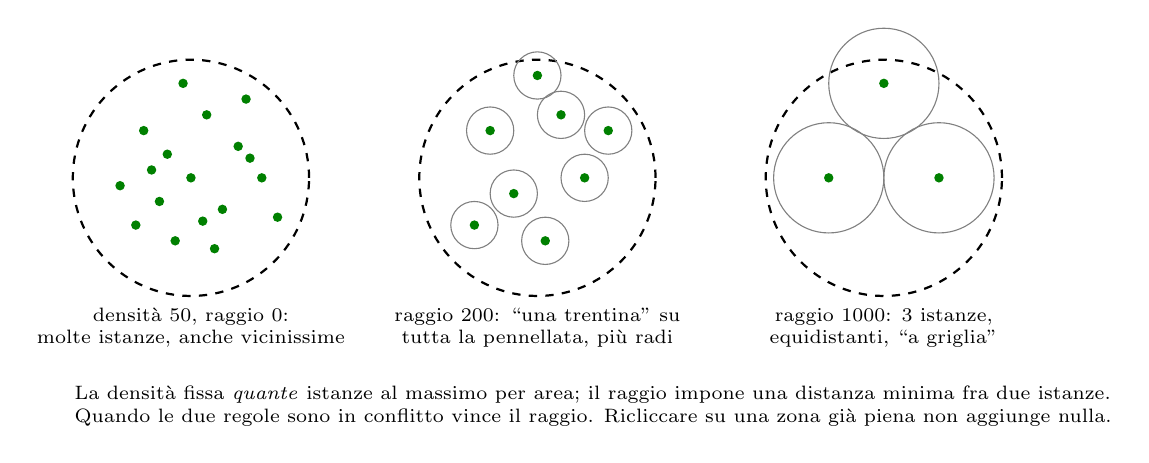
\begin{tikzpicture}[font=\scriptsize, x=1cm, y=1cm]
  % pannello 1: raggio 0
  \draw[thick, dashed] (1.6,1.6) circle (1.5);
  \foreach \p in {(1.0,2.2),(1.3,1.9),(1.8,2.4),(2.2,2.0),(0.7,1.5),(1.2,1.3),(1.6,1.6),(2.0,1.2),(2.5,1.6),(1.4,0.8),(1.9,0.7),(0.9,1.0),(2.3,2.6),(1.5,2.8),(2.7,1.1),(1.1,1.7),(1.75,1.05),(2.35,1.85)}
    {\fill[green!50!black] \p circle (0.06);}
  \node[align=center] at (1.6,-0.3) {densità 50, raggio 0:\\molte istanze, anche vicinissime};
  % pannello 2: raggio medio
  \begin{scope}[xshift=4.4cm]
    \draw[thick, dashed] (1.6,1.6) circle (1.5);
    \foreach \p in {(1.0,2.2),(1.9,2.4),(1.3,1.4),(2.2,1.6),(0.8,1.0),(1.7,0.8),(2.5,2.2),(1.6,2.9)}
      {\fill[green!50!black] \p circle (0.06); \draw[gray] \p circle (0.3);}
    \node[align=center] at (1.6,-0.3) {raggio 200: ``una trentina'' su\\tutta la pennellata, più radi};
  \end{scope}
  % pannello 3: raggio grande
  \begin{scope}[xshift=8.8cm]
    \draw[thick, dashed] (1.6,1.6) circle (1.5);
    \foreach \p in {(0.9,1.6),(2.3,1.6),(1.6,2.8)}
      {\fill[green!50!black] \p circle (0.06); \draw[gray] \p circle (0.7);}
    \node[align=center] at (1.6,-0.3) {raggio 1000: 3 istanze,\\equidistanti, ``a griglia''};
  \end{scope}
  \node[align=left, anchor=west] at (0,-1.3) {La densità fissa \emph{quante} istanze al massimo per area; il raggio impone una distanza minima fra due istanze.\\Quando le due regole sono in conflitto vince il raggio. Ricliccare su una zona già piena non aggiunge nulla.};
\end{tikzpicture}
\caption{Densità e raggio nel Foliage Mode, con i numeri delle prove della lezione. Il
cerchio tratteggiato è il pennello; i cerchi grigi attorno alle istanze rappresentano il
raggio minimo. Ricostruzione schematica: le posizioni dei punti sono indicative.}
\label{ue15:fig:raggio}
\end{figure}

\paragraph{Approfondimento: come piazza il pennello.} Il comportamento visto a lezione è
coerente con il modo in cui il Foliage Mode lavora. A ogni pennellata calcola quante istanze
dovrebbero esserci nell'area del pennello in base a \emph{Density} (istanze per
1000$\times$1000 unità, cioè per 10$\times$10 metri) e alla \emph{Paint Density}; conta quelle
già presenti dello stesso tipo e aggiunge solo le mancanti, scartando ogni posizione
candidata che cada entro il \emph{Radius} di un'istanza esistente. Da qui le tre cose
osservate: ricliccare non aggiunge nulla quando la zona è ``piena''; togliendo il raggio si
riempiono i buchi che il raggio aveva scartato; con un raggio grande la densità teorica non
si raggiunge mai, e le istanze si dispongono a distanza quasi costante. Il raggio è anche il
modo più semplice per evitare alberi compenetrati, il problema che Totten chiama
\emph{casualità percepita} (si veda l'approfondimento della
sezione~\ref{ue15:sec:selezione}). Funzionamento generale dell'engine.

% ---------------------------------------------------------------------
\section{Le altre impostazioni: pendenza, altezza, mobilità, collisioni}
\label{ue15:sec:altre}

\paragraph{Align to Normal e Align Max Angle.} \textbf{Align to Normal} decide se le istanze
``sono allineate alla normal su cui sono applicate''. \textbf{Align Max Angle} è ``quanto si
inclinano per aggiustarsi alla singola pendenza'' (il docente in un primo momento lo confonde
con il parametro successivo e si corregge: ``no, aspetta, mi sa che\dots'').

\paragraph{Ground Slope Angle.} È ``il range in cui il foliage verrà piazzato'': l'angolo
minimo e massimo della superficie su cui un'istanza può comparire. Il docente dipinge l'erba
su un pendio (dopo un momento di confusione: ``stavo modificando ancora le cose dell'albero
invece era l'erba che andava modificata; ci ho cliccato sopra, pensavo di averla selezionata e
invece non era selezionata'', ``è il tipo di cose che vi capiterà sicuramente ogni tanto''). Con
l'intervallo di default, fino a 180, l'erba va ``anche sulla parete rocciosa''. ``Poi sta a voi
decidere se volete che il foliage venga piazzato anche lì oppure no.'' Con un massimo di
\textbf{45} gradi, l'erba compare ``soltanto nelle parti della slope che erano sotto i 47
gradi'' (il docente dice 47 avendo impostato 45: con ogni probabilità è un lapsus), e si
ammucchia nei punti meno ripidi. Abbassando ancora, ``neanche su questa cunetta è stata
messa, perché l'angolazione è troppo alta''. Un uso: mettere attorno alla base del
``montarozzo'' dell'erba a mano, ``per far vedere che un minimo c'è stata un'espansione
erbosa'', senza che salga sulle pareti; ``anche troppo preciso, devo dire''. Il docente lo
rimette a 45 (figura~\ref{ue15:fig:slope}).

\begin{figure}[htbp]
\centering
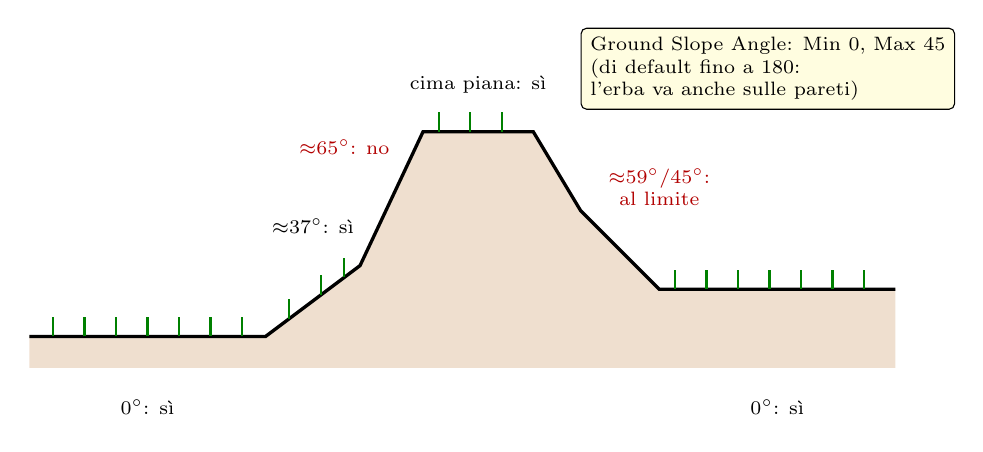
\begin{tikzpicture}[font=\scriptsize, x=1cm, y=1cm]
  \fill[brown!25] (0,0) -- (3,0) -- (4.2,0.9) -- (5.0,2.6) -- (6.4,2.6) -- (7.0,1.6) -- (8.0,0.6) -- (11,0.6) -- (11,-0.4) -- (0,-0.4) -- cycle;
  \draw[very thick] (0,0) -- (3,0) -- (4.2,0.9) -- (5.0,2.6) -- (6.4,2.6) -- (7.0,1.6) -- (8.0,0.6) -- (11,0.6);
  % erba
  \foreach \x in {0.3,0.7,...,2.9} {\draw[green!50!black, thick] (\x,0) -- (\x,0.25);}
  \foreach \x in {3.3,3.7,4.0} {\draw[green!50!black, thick] (\x,{0.75*(\x-3)}) -- (\x,{0.75*(\x-3)+0.25});}
  \foreach \x in {5.2,5.6,...,6.3} {\draw[green!50!black, thick] (\x,2.6) -- (\x,2.85);}
  \foreach \x in {8.2,8.6,...,10.9} {\draw[green!50!black, thick] (\x,0.6) -- (\x,0.85);}
  \node[align=center] at (1.5,-0.9) {0$^\circ$: sì};
  \node[align=center] at (3.6,1.4) {$\approx$37$^\circ$: sì};
  \node[align=center, red!70!black] at (4.0,2.4) {$\approx$65$^\circ$: no};
  \node[align=center] at (5.7,3.2) {cima piana: sì};
  \node[align=center, red!70!black] at (8.0,1.9) {$\approx$59$^\circ$/45$^\circ$:\\al limite};
  \node[align=center] at (9.5,-0.9) {0$^\circ$: sì};
  \node[align=left, anchor=west, draw, rounded corners=2pt, fill=yellow!12] at (7.0,3.4) {Ground Slope Angle: Min 0, Max 45\\(di default fino a 180:\\l'erba va anche sulle pareti)};
\end{tikzpicture}
\caption{Il Ground Slope Angle di un foliage type. Con un massimo di 45 gradi il pennello
piazza istanze solo dove la superficie è inclinata meno di 45 gradi rispetto all'orizzontale;
le pareti restano spoglie. Gli angoli indicati sono esempi. Ricostruzione schematica.}
\label{ue15:fig:slope}
\end{figure}

\paragraph{Height.} Il range d'altezza in cui il foliage può essere piazzato. Di default va
da meno a più infinito (``da meno a più''); con \textbf{0 -- 10}, ``appena andiamo sopra i 10
d'altezza, lui smette di piazzarla''.

\paragraph{Mobility.} Come per le luci: \textbf{Static}, ``più veloci da renderizzare'', che
``funzionano col baking'', o \textbf{Movable}, ``completamente dinamiche'', con le luci che
``reagiscono in tempo reale'', ``ma è più lento da gestire''.

\paragraph{Cull Distance.} ``La distanza massima da cui non smettono di essere renderizzate.''
Allontanandosi, ``tutto il resto del foliage è sparito'', quello del materiale, ``ma questo è
rimasto, perché c'è zero di cull distance'': ``non ha massimo e minimo, esiste e basta, non viene
tagliato, è sempre renderizzato''. ``Gestitelo sulla base della grandezza della vostra scena.''

\paragraph{Le ombre e il dressing.} \emph{Cast Shadow}, ombre dinamiche e statiche,
\emph{Affect Dynamic Lighting}: ``tutti i check che potete gestirvi per la resa estetica con
la luce''. L'erba del pacchetto ``è fatta apposta per non castare ombre''. Il foliage si può
dipingere anche \emph{sopra} le mesh: il docente mette dell'erba sopra una struttura della
base, e immagina ``un mondo post apocalittico con una pompa di benzina abbandonata'' (``non so
perché mi ha fatto pensare alla pompa di benzina''), con l'erba che ci cresce sopra e ``dei
\emph{vine} che scendono giù'' (delle liane, dei rampicanti).

\paragraph{Collision Presets.} ``E poi abbiamo i preset delle collisioni.'' La frase del docente
è ambigua (``di default tutto il foliage è impostato a una collisione, che nel caso dell'erba
ci fa anche comodo, perché noi non vogliamo che ci sia l'erba e poi ci inciampiamo sopra''):
il senso è che \emph{per l'erba} si vuole che non ci siano collisioni. ``Quando andiamo a
mettere gli alberi, però, dobbiamo assicurarci che lì sia tutto funzionale, che le collisioni
ci siano, perché altrimenti possiamo passarci attraverso.''

\paragraph{L'ingresso della base.} Prima degli alberi il docente sistema l'erba davanti alla
base: ``il nostro personaggio uscirà da lì e si trova prima l'erbetta che va a gradiente, poi
c'è il folto''.

\paragraph{Approfondimento: le impostazioni del foliage type.} Qualche precisazione sui
parametri visti. \emph{Ground Slope Angle} confronta la normale della superficie con la
verticale, come il World Aligned Blend dell'automaterial: le due cose si possono far
coincidere, così che il foliage manuale non finisca dove il materiale mette la roccia.
\emph{Height} usa la quota assoluta del mondo in centimetri, quindi ``0 -- 10'' è una fascia di
dieci centimetri sopra lo zero del mondo, utile per esempio per non piantare canne sopra il
livello dell'acqua. \emph{Cull Distance} ha un minimo e un massimo: fra i due le istanze
sfumano, e con entrambi a 0 il culling per distanza è disattivato, come visto. I
\emph{Collision Presets} del foliage type (\emph{Body Instance}) decidono come le istanze
\emph{rispondono} alle collisioni; perché ci sia una collisione, però, la mesh deve averne una
(la sezione successiva lo mostra). Romero e Sewell descrivono nel capitolo 14 (``Math and
Trace Nodes'') la tabella delle \emph{Collision Responses}: ogni oggetto ha un \emph{Object
Type} e una risposta (\emph{Ignore}, \emph{Overlap} o \emph{Block}) per ogni canale, con dei
preset come \emph{BlockAll}, \emph{OverlapAllDynamic} e \emph{Pawn}, oppure
\emph{Custom\ldots}; nel capitolo 5 impostano \emph{BlockAllDynamic} su un oggetto
interattivo. Le stesse regole valgono per le istanze del foliage.

% ---------------------------------------------------------------------
\section{Gli alberi e le collisioni}
\label{ue15:sec:alberi}

\paragraph{Le impostazioni dell'albero.} ``Togliamo l'erba, perché sennò dipingiamo anche
l'erba insieme agli alberi.'' Le impostazioni del pacchetto: \textbf{Density 1}, ``abbastanza
sparsi'', raggio 0: ``ci può stare''. Il docente ne mette una fila all'ingresso, ``una piccola
radura''. Gli alberi sono di taglie diverse (\textbf{Scale} da 1 a 3: ``con l'albero funziona
meglio, dà un'idea migliore''; c'è l'albero ``di base'' e ``l'albero grosso'') e ruotati in
maniera diversa: lo Z Offset è 0, ma c'è il \textbf{Random Yaw}, ``una rotazione randomica
sull'asse verticale''. Togliendolo, ``gli alberi vanno tutti nella stessa direzione, sono tutti
curvi in quella direzione, verso sinistra''; rimettendolo, ``iniziano a ruotare''. (Un albero
``si è rifiutato di essere cancellato''.)

\paragraph{Alberi dalle pareti.} Lasciando il Ground Slope Angle ampio e Align to Normal
attivo, si possono piantare alberi su una parete: ``alberi che escono dalle pareti, non so
perché dovreste volerlo fare, ma lo potete fare''. Per esempio ``un percorso di alberi tutto
attaccato sul lato della parete, che potete utilizzare come percorso per un platform''.
Togliendo Align to Normal ``ve li spawna dritti''. Con gli alberi l'allineamento ``non funziona
granché bene'', ``ma per esempio con dei cespugli o dei funghi parassiti'' sì.

\paragraph{La collisione strana.} Le collisioni dell'albero sono \textbf{Block All}. ``Col
nostro robottino andiamo all'avventura'': ``siamo alti quanto l'erba'' (bisognerà abbassarla).
In Play si riesce a passare dentro gli alberi, almeno in parte: ``hanno una strana
collisione''. Prima di guardare, il docente chiarisce ``una grossa cosa'' sulle collisioni:
``questo parametro non determina se l'oggetto avrà collisioni o meno; determina se le
collisioni dell'oggetto sono attive o meno, e per cosa sono attive''. La prova: Block All
sull'\textbf{erba}. ``Sono positivamente sicuro che potremo comunque camminare dentro l'erba'':
ed è così (``se dovessimo esplorare un open world del genere, il nostro personaggio dovrebbe
muoversi più veloce di così''). Il motivo è nella static mesh di base: nello Static Mesh
Editor, con \textbf{Show Simple Collision}, ``non ci sono simple collision, quindi non c'è
nulla da attivare''. ``Vi capiterà di mettere degli asset in scena, iniziare a giocare e
passarci attraverso, perché magari quegli asset sono stati importati o esportati senza le
collisioni''; e anche impostando ``le collisioni che bloccano tutto, o che bloccano solo i
proiettili'', ``lui comunque non può bloccare, perché non c'è nulla da bloccare''.

\paragraph{L'albero, dentro.} Aprendo la mesh dell'albero: ``ah, geniale. L'hanno messa dalla
parte sbagliata.'' Le forme della collisione semplice (``diversi pezzi'') sono ruotate rispetto
al tronco, ``credo che l'abbiano importato proprio con la collisione sbagliata''. Si possono
selezionare tutte e ruotare ``dalla parte corretta''; ``anche se sono proprio strane'',
sbagliate anche nelle proporzioni. Tre strade:
\begin{enumerate}
  \item \textbf{ruotare} le forme esistenti, come fa il docente (``tanto il nostro giocatore
        non andrà mai a collidere lassù, a meno che non vogliamo che lo faccia'');
  \item \textbf{eliminare} le simple collision e scegliere \textbf{Use Complex Collision As
        Simple}: la collisione prende ``esattamente i poligoni dell'albero''. ``Chiaramente
        questa cosa è pesante, però vi risolve il problema di dover fare le collisioni a
        mano'';
  \item \textbf{rifarle} a mano con forme semplici: ``vi basterebbe prendere un cilindro,
        metterlo in diagonale, e qui sopra metterci un piano circolare''. Il docente aggiunge
        una \textbf{capsula}, la fa più piccola e più stretta, la ruota lungo il tronco, e
        sopra una \textbf{box piatta}, ``in modo che il giocatore possa salire sulla cima
        dell'albero e rimanerci sopra'' (figura~\ref{ue15:fig:collisione}).
\end{enumerate}
Se si vuole che il personaggio salti da un albero all'altro o percorra la parete passando sui
tronchi, ``non potete fare questa cosa'' con la collisione originale: ``dovete togliere queste
collisioni e rifarle''.

\begin{figure}[htbp]
\centering
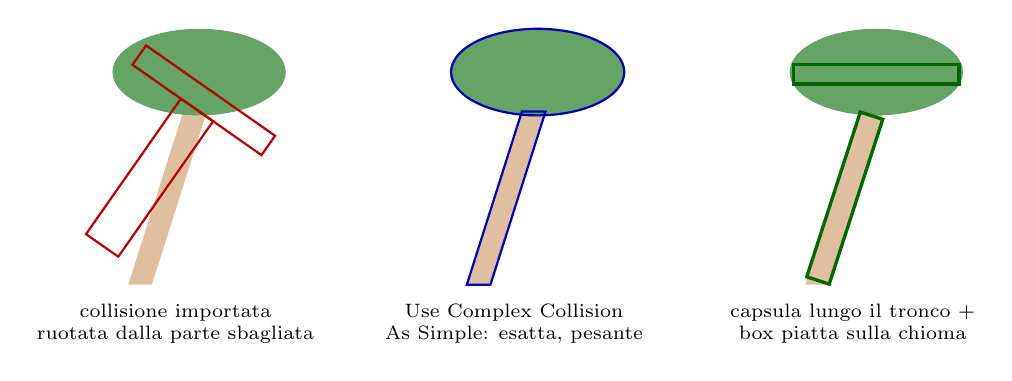
\begin{tikzpicture}[font=\scriptsize, x=1cm, y=1cm]
  % albero originale
  \begin{scope}
    \fill[brown!50] (0.9,0) -- (1.2,0) -- (1.9,2.2) -- (1.6,2.2) -- cycle;
    \fill[green!40!black!60] (1.8,2.7) ellipse (1.1 and 0.55);
    \draw[red!70!black, thick, rotate around={-35:(1.2,1.4)}] (0.95,0.3) rectangle (1.45,2.4);
    \draw[red!70!black, thick, rotate around={-35:(1.2,1.4)}] (0.2,2.4) rectangle (2.2,2.7);
    \node[align=center] at (1.5,-0.5) {collisione importata\\ruotata dalla parte sbagliata};
  \end{scope}
  % complex as simple
  \begin{scope}[xshift=4.3cm]
    \fill[brown!50] (0.9,0) -- (1.2,0) -- (1.9,2.2) -- (1.6,2.2) -- cycle;
    \fill[green!40!black!60] (1.8,2.7) ellipse (1.1 and 0.55);
    \draw[blue!70!black, thick] (0.9,0) -- (1.2,0) -- (1.9,2.2) -- (1.6,2.2) -- cycle;
    \draw[blue!70!black, thick] (1.8,2.7) ellipse (1.1 and 0.55);
    \node[align=center] at (1.5,-0.5) {Use Complex Collision\\As Simple: esatta, pesante};
  \end{scope}
  % capsula + box
  \begin{scope}[xshift=8.6cm]
    \fill[brown!50] (0.9,0) -- (1.2,0) -- (1.9,2.2) -- (1.6,2.2) -- cycle;
    \fill[green!40!black!60] (1.8,2.7) ellipse (1.1 and 0.55);
    \draw[green!40!black, very thick, rotate around={-18:(1.4,1.1)}] (1.25,0.0) rectangle (1.55,2.2);
    \draw[green!40!black, very thick] (0.75,2.55) rectangle (2.85,2.8);
    \node[align=center] at (1.5,-0.5) {capsula lungo il tronco +\\box piatta sulla chioma};
  \end{scope}
\end{tikzpicture}
\caption{Tre modi di sistemare la collisione dell'albero di StackOBot visti a lezione:
ruotare le forme importate male, usare la geometria della mesh come collisione, oppure
rifare la collisione con una capsula (qui disegnata come un rettangolo inclinato) e una box
piatta su cui il giocatore può stare in piedi. Ricostruzione schematica.}
\label{ue15:fig:collisione}
\end{figure}

\paragraph{La domanda sulle collisioni a senso unico.} Uno studente ha una domanda ``fuori
tema'': ``le collisioni che funzionano da un solo lato?'' Gli è venuto in mente un gioco (``PIC''
nella trascrizione: con ogni probabilità \emph{PEAK}, il gioco cooperativo di arrampicata, ma
il nome non è certo) in cui ``puoi salire sugli alberi e puoi attraversare le foglie da sotto,
ma non puoi attraversarle da sopra''. Il docente non ci ha mai pensato: ``probabilmente dipende
dal modo in cui è codificato quel tipo di interazione''. ``Gli dici che se stai andando in una
direzione non deve contare quella collisione, se stai andando nell'altra deve contarla.
Penso, non lo so, a naso direi che è questo.'' Non ha giocato il gioco.

\paragraph{No Collision sovrascrive.} Rimesso tutto com'era, con le collisioni girate ``dalla
parte giusta'', il docente imposta \textbf{No Collision} nel foliage type dell'albero: ``lui
sovrascrive il fatto che ha delle collisioni''. In Play ci si passa attraverso, ``perché l'asset
del foliage non ha collisioni''. Con \textbf{Custom} si sceglie che cosa bloccano: ``se bloccano
la camera, se bloccano i proiettili, se bloccano il pawn''. ``Di base, il Block All andrà
bene.''

\paragraph{Approfondimento: collisione semplice, complessa e a senso unico.} Una static mesh
ha due rappresentazioni di collisione. La \emph{simple collision} è fatta di primitive
(box, sfere, capsule, convessi) ed è quella usata dalla fisica e dal movimento del
personaggio: è economica, ma va costruita (nello Static Mesh Editor, menu
\emph{Collision}: \emph{Add Box}, \emph{Add Capsule}, \emph{Auto Convex Collision}\dots)
o importata dal programma di modellazione. La \emph{complex collision} è la mesh stessa,
triangolo per triangolo, usata di solito solo per le tracce precise. \emph{Collision
Complexity: Use Complex Collision As Simple} fa usare la seconda anche per la fisica: comoda,
ma costosa su mesh dense e, per i corpi simulati, non utilizzabile. Le collisioni ``a senso
unico'' delle piattaforme attraversabili da sotto non sono una proprietà della collisione
in Unreal: si ottengono via codice, per esempio con un volume sotto la piattaforma che, quando
il personaggio sale, gli fa ignorare il canale della piattaforma (\emph{Ignore}) e lo
ripristina quando il personaggio è sopra, oppure controllando la velocità verticale; è
proprio la risposta ``a naso'' del docente. Le risposte \emph{Ignore}/\emph{Overlap}/\emph{Block}
per canale sono quelle della tabella del capitolo 14 di Romero e Sewell; il resto è
funzionamento generale dell'engine.

% ---------------------------------------------------------------------
\section{Selezionare, rifinire e il foliage non naturale}
\label{ue15:sec:selezione}

\paragraph{Il cespuglio a mano.} ``Lo stesso con gli altri oggetti.'' Il cespuglio del
pacchetto spawna poco; è ``un tipo di asset che io, piuttosto che metterlo così, farei
\textbf{single} e andrei a posizionare a mano'': ``voglio che queste cose stiano molto
ammucchiate vicino agli alberi''. Le dimensioni sono comunque casuali, ``forse troppo varie
per i miei gusti''. Allo stesso modo si fa ``un percorso alberato'', con alberi a destra e a
sinistra, che ``fa comunque parte del foliage'' e si integra con il resto.

\paragraph{Gli strumenti di selezione.}
\begin{itemize}
  \item \textbf{Select}: si prende ``il singolo pezzo di foliage'' e lo si sposta (``no, no,
        quest'albero non deve stare proprio lì, deve stare qui''), ``un po' tipo selection mode,
        ma con tutti gli asset che rimangono all'interno del foliage''. Tornando in Selection
        Mode e cliccando, invece, si seleziona tutto il foliage actor. (Il docente trova
        nell'Outliner anche delle istanze che non si aspettava, ``saranno delle cose che
        c'erano prima'', e non approfondisce.)
  \item \textbf{Select All} e \textbf{Deselect}: tutte le istanze dei tipi attivi, da
        muovere insieme.
  \item \textbf{Select Invalid}: ``mi porta automaticamente alle instance che sono invalide,
        quindi quelle che vanno modificate''.
  \item \textbf{Lasso}: ``funziona un po' tipo Photoshop'': invece di cliccare, si evidenzia
        una zona. Vale solo per i tipi spuntati: ``qui ci sono sempre attivi soltanto gli
        alberi, quindi se voglio fare questa cosa devo prendere anche questi''.
  \item \textbf{Remove}: ``questi alberi qua non mi piacciono'': elimina tutto ciò che è stato
        evidenziato.
  \item un ultimo strumento, ``stessa cosa con i raise, però è un discorso un po' diverso, poi
        modifica piano piano'': il nome non è ricostruibile con certezza (con ogni probabilità
        \emph{Reapply}, che riapplica le impostazioni del foliage type alle istanze già
        dipinte).
\end{itemize}

\paragraph{Non deve essere naturale.} ``È tendenzialmente uno strumento che utilizzate
principalmente per motivi estetici.'' E ``non deve essere necessariamente naturale'': si può
usare ``con ogni mesh che voglio''. ``Se io voglio riempire la scena di robottini, lo posso
fare''; una scena in metropolitana con il pavimento pieno di ``cartacce, plastiche, cose
varie''. ``È un po' un pennello con cui piazzare rapidamente tutta una serie di oggetti.''

\paragraph{Le rocce sotto lo zero.} Le rocce dipinte ``appena si avvicinano allo zero
impazziscono; invece sopra sono perfette''. Consiglio: ``mettete il piano di base leggermente
più alto dello zero''. Spostando una roccia, il materiale cambia: ``cambia sulla base
dell'altezza''; ruotandola, ``così diventa una parete rocciosa''. ``È un po' strano che abbiano
scelto di fare un materiale dinamico così per un oggetto standard.'' Aprendo il materiale
(``più complesso di quello che pensavo''), il docente legge nomi come \emph{Virtual
Texture}, \emph{World Position} e una ``variation'' (la trascrizione dice ``part time, drop
variation'', non ricostruibile): ``hanno provato a fare una roba carina'' per avere un
materiale dinamico, ``tipo il \textbf{vertex painting}'', e per ``blendare la mesh con
l'oggetto del landscape'' quando si dipinge il materiale del landscape. Ma ``volendo, potete
fare anche letteralmente solo una texture di roccia'' con le sue mappe, ``e avete comunque una
roccia''.

\paragraph{Approfondimento: la casualità percepita.} Il Foliage Mode rende facilissimo
spargere oggetti a caso, ed è proprio il rischio che Totten descrive nel capitolo 8
(``Possibility Spaces and Worldbuilding''): in natura alberi, rocce e scogliere si dispongono
nel tempo in modi non pianificati, e i designer alle prime armi piazzano alberi, rocce ``e
perfino edifici'' a caso sulla mappa, ``ignari dell'importanza della loro posizione''; il
risultato è una \emph{casualità percepita} che non dice nulla al giocatore. ``Dirigere lo
sguardo verso elementi scenici piazzati con cura'' è il modo in cui il giocatore capisce il
mondo. In pratica: il pennello per la massa (l'erba, il bosco di sfondo), lo \emph{Single
Instance Mode} e il \emph{Select} per gli elementi che contano (l'albero isolato che fa da
landmark, i cespugli che incorniciano un passaggio), che è esattamente il modo di lavorare del
docente con i cespugli. Nel capitolo 3 (``Basic Gamespaces'') Totten aggiunge che un cambio
nel tipo di vegetazione segnala il passaggio a una zona nuova, come un cambio di texture sul
terreno. Sul materiale delle rocce: un materiale che campiona texture in world space
(\emph{world aligned}) cambia aspetto quando l'oggetto si sposta o ruota, perché la texture
resta ferma nel mondo mentre la mesh si muove; e un calcolo basato sulla quota assoluta (per
esempio per sfumare la base nella sabbia o nell'umidità) produce effetti strani sotto lo
zero, se chi l'ha fatto ha supposto che il terreno stia sopra. Funzionamento generale
dell'engine; il grafo del materiale non è stato verificato nel capitolo.

% ---------------------------------------------------------------------
\section{La domanda sui mondi procedurali}
\label{ue15:sec:procedurale}

\paragraph{Landscape o mesh?} ``Ci sono domande?'' Uno studente: ``i mondi che si generano
automaticamente usano il landscape o le mesh?'' ``Tipo le robe procedurali? Tendenzialmente
dipende.'' ``È più comodo farlo con le mesh, perché puoi farti un \textbf{array} di oggetti e
puoi piazzarli secondo dei criteri che hai scelto tu.'' Ma ``l'ultima volta che ho lavorato
con qualcosa di procedurale era un sacco di tempo fa'', e magari ci sono ``nuovi nodi'' o
``feature che Unreal ha inserito'' che il docente non conosce. Il consiglio: cercare sullo store
``qualche pacchetto che parla di asset procedurali, non modulari, proprio procedurali, che ha
dei sistemi di proceduralizzazione'', e ``ti studi un po' loro come le fanno''. ``Fab, intendi,
giusto?'' ``Sì, su Fab. Ai miei tempi non si chiamava Fab, mi sento vecchio.''

\paragraph{Lo strumento che non si trova.} Parlando di procedurale, il docente ricorda ``un
tool che io non ho mai usato, che dovrebbe essere relativamente nuovo'': ``una specie di box
all'interno della quale possono essere impostati dei parametri, e spostando questa box e
ingrandendola, lui va a piazzare quel tipo di foliage nel volume che c'è all'interno''. Lo
cerca fra i tipi di asset del menu \emph{Foliage} (c'è lo \emph{Static Mesh Foliage}, ``questo
qui è letteralmente il nuovo, ma non è quello che voglio''), non lo trova, e ipotizza che
fosse ``un plugin''. ``Me lo devo vedere meglio.''

\paragraph{Sprite e flipbook.} Nello stesso menu ``vi potete vedere tutti i tipi di asset che
possono essere creati'', anche gli \textbf{sprite} e i \textbf{flipbook}: ``carini se volete
fare, che ne so, un menu animato''. ``Visto che avete fatto la roba col menu, con un flipbook
potete andare a fare l'animazione del menu.''

\paragraph{Approfondimento: generazione procedurale in Unreal.} Lo strumento descritto dal
docente corrisponde con ogni probabilità a uno di due sistemi, ed entrambi si attivano da
plugin. Il primo è il \emph{Procedural Foliage Spawner} con il suo \emph{Procedural Foliage
Volume}: si definisce quali foliage type crescono, con quali regole di competizione e di
età, e si fa ``simulare'' la crescita dentro il volume (è una funzione sperimentale,
\emph{Procedural Foliage}, da abilitare nelle impostazioni dell'editor). Il secondo, più
recente e oggi il sistema di riferimento, è il framework \emph{PCG} (\emph{Procedural
Content Generation}), con il \emph{PCG Volume} e un grafo a nodi che campiona superfici,
filtra i punti per pendenza o altezza e vi genera mesh: il plugin si chiama
\emph{Procedural Content Generation Framework}. La risposta del docente sulle mesh resta
valida: anche il PCG, alla fine, produce istanze di static mesh. Romero e Sewell, nel
capitolo 19 (``Procedural Generation''), definiscono la generazione procedurale come ``un
metodo per creare il contenuto del livello usando script invece che a mano'', utile per
evitare compiti ripetitivi; la costruiscono con il \emph{Construction Script}, un
\emph{Instanced Static Mesh Component} e dei cicli \emph{For Loop} che dispongono righe di
istanze, e poi con le \emph{Blueprint Spline} per piazzare actor lungo un percorso. Gli
sprite e i flipbook appartengono a \emph{Paper2D}, il sistema 2D dell'engine: un flipbook è
una sequenza di sprite riprodotta a una certa velocità. Fab è lo store di Epic che dal 2024
ha sostituito l'Unreal Engine Marketplace, quello usato nel capitolo 9 del libro per
importare l'\emph{Animation Starter Pack}.

% ---------------------------------------------------------------------
\section{Il Niagara e il Post Process Volume}
\label{ue15:sec:postprocess}

``Come ho detto, ci abbiamo una decina di minuti.'' In quella decina di minuti si potrebbe
``buttare un occhio'' sul post process, ``visto che ci siamo''.

\paragraph{Un'occhiata al Niagara.} Prima, ``al volo'', il Niagara: ``è proprio un editor a
parte''. Creando un \textbf{Niagara System} si sceglie fra ``tutte le varie forme, modi, colori,
possibilità'' dei \emph{preset}; il docente prende una \textbf{Fountain}, ``la base della
cosa''. Dentro c'è ``tutto un sistema così, con la timeline, con degli \textbf{emitter}, tutte
cose''. ``È una roba un po' complicata, magari ce la vediamo alla prossima lezione se
riusciamo.''

\paragraph{Dove si trova il post process.} Dal \textbf{Place Actors}, nella categoria
\textbf{Volumes}, ``tra le varie cose'' (``insieme a tutta una serie di altre cose molto, molto
carine'') c'è il \textbf{Post Process Volume}: ``il nostro quadratone''.

\paragraph{Che cos'è.} ``È un volume all'interno del quale voi andate ad applicare delle
modifiche alla lente della telecamera, fondamentalmente.'' ``Voi andate a modificare il modo in
cui le cose appaiono, non il modo in cui le cose sono.'' Le stesse ``lenti'' esistono anche su
una \textbf{Camera Actor}: nei suoi Details, nella sezione \emph{Post Process}, ``abbiamo
diverse lenti che possiamo andare a modificare'', e queste modifiche ``si applicano solo alla
singola telecamera''. Il volume invece applica gli effetti \emph{al suo interno}.

\paragraph{Le transizioni.} ``Vi siete mai chiesti come fanno a fare quegli effetti per cui
quando entri o esci da una casa il bloom della luce è particolarmente forte e poi si attenua?
O com'è possibile che la luce fuori era molto forte, io entro dentro una grotta e piano piano
la luce diventa più tenue e cambia colore?'' ``È perché il post process ha degli effetti di
transizione fra l'interno e l'esterno.'' Si possono piazzare più Post Process Volume con
effetti diversi, e passando dall'uno all'altro cambia ``il modo in cui la mia telecamera va a
gestire le cose''.

\paragraph{I volumi annidati.} Si può anche mettere un post process dentro un altro, ``una roba
complicata che vi sconsiglierei di fare'': il volume interno ``calcola tutto quello che lui
deve calcolare e in più ci applica anche quello'' dell'esterno. L'esempio: il volume interno
rende la scena gialla (\emph{color correction}), quello esterno blu; stando nell'interno ``vediamo
tutto verde, perché lui somma la color correction dei due post process''. ``Per cui diventa molto
complicato capire cosa vogliamo fare.'' (Figura~\ref{ue15:fig:postprocess}.)

\paragraph{Un solo volume per tutto: Infinite Extent.} ``Se voglio un unico post process che
determina il modo in cui la scena viene vista, devo renderlo incredibilmente grande?'' No:
nei Details del volume (``le stesse lenti che aveva il camera actor, con qualche opzione in
più'') si cerca \emph{infinite} e si trova \textbf{Infinite Extent (Unbound)}: ``quando questa
casella viene spuntata, il volume copre tutto il mondo, non solo l'area all'interno'', e i
cambiamenti ``vengono visti allo stesso modo in tutta la zona''. Per ora la si toglie.

\paragraph{Le lenti, per la prossima volta.} ``Non so quanto senso abbia iniziare a parlare
delle lenti: ci abbiamo 5 minuti, e ogni lente ha un sacco di parametri.'' Due accenni: il
\textbf{Bloom}, ``abbastanza semplice'', ``quello che serve per i god shaft'' di cui si parlava
prima; e la \textbf{Chromatic Aberration}: ``occhio, che fa male agli occhi''. Il resto alla
prossima lezione.

\begin{figure}[htbp]
\centering
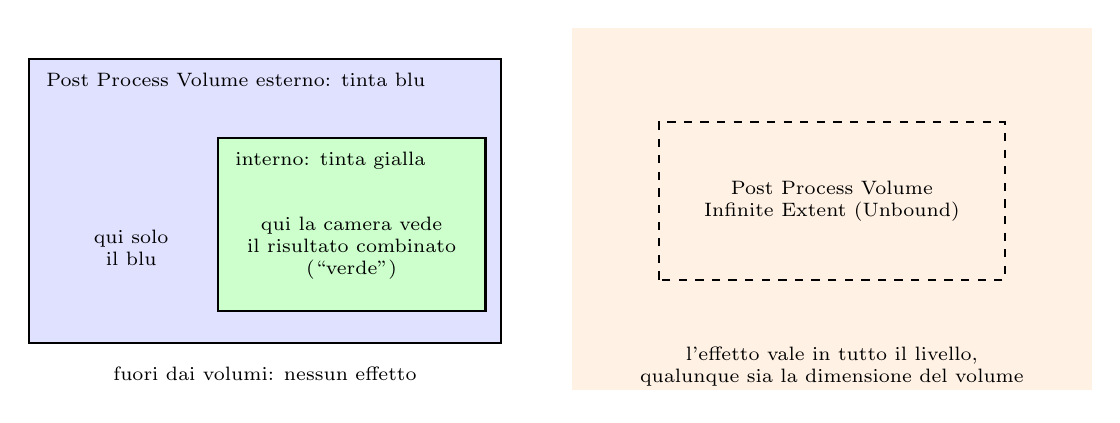
\begin{tikzpicture}[font=\scriptsize, x=1cm, y=1cm]
  \draw[thick, fill=blue!12] (0,0) rectangle (6,3.6);
  \node[anchor=north west] at (0.1,3.55) {Post Process Volume esterno: tinta blu};
  \draw[thick, fill=green!20] (2.4,0.4) rectangle (5.8,2.6);
  \node[anchor=north west, align=left] at (2.5,2.55) {interno: tinta gialla};
  \node[align=center] at (4.1,1.2) {qui la camera vede\\il risultato combinato\\(``verde'')};
  \node[align=center] at (1.3,1.2) {qui solo\\il blu};
  \node[align=center] at (3,-0.4) {fuori dai volumi: nessun effetto};
  % unbound
  \begin{scope}[xshift=7.2cm]
    \fill[orange!10] (-0.3,-0.6) rectangle (6.3,4.0);
    \draw[thick, dashed] (0.8,0.8) rectangle (5.2,2.8);
    \node[align=center] at (3,1.8) {Post Process Volume\\Infinite Extent (Unbound)};
    \node[align=center] at (3,-0.3) {l'effetto vale in tutto il livello,\\qualunque sia la dimensione del volume};
  \end{scope}
\end{tikzpicture}
\caption{A sinistra, due Post Process Volume annidati: dentro il volume interno la camera
riceve l'effetto di entrambi, come nell'esempio del docente (giallo e blu che danno verde). A
destra, un volume con \emph{Infinite Extent (Unbound)}, che vale per tutto il livello.
Ricostruzione schematica.}
\label{ue15:fig:postprocess}
\end{figure}

\paragraph{Approfondimento: come si combinano i post process.} Il comportamento dei volumi
sovrapposti è un po' più ordinato della ``somma'' descritta a lezione. Ogni Post Process
Volume ha una \emph{Priority}, un \emph{Blend Weight} (da 0 a 1) e un \emph{Blend Radius}, la
distanza dal bordo entro cui l'effetto sfuma: è il Blend Radius che produce le transizioni
graduali fra esterno e grotta. Ogni volume modifica solo le proprietà la cui casella è
spuntata; quando la camera è dentro più volumi, Unreal li applica in ordine di priorità, e
per ogni proprietà il valore del volume a priorità più alta si \emph{mescola} con quello già
calcolato secondo il suo Blend Weight (con peso 1 lo sostituisce). Se due volumi cambiano
proprietà diverse, si vedono entrambe le modifiche; se cambiano la stessa con peso minore di
1, si ottiene una via di mezzo: in questo senso le due tinte possono dare un colore
combinato. Il consiglio del docente resta buono: pochi volumi, priorità esplicite, e di solito
un volume \emph{Unbound} a priorità bassa per l'aspetto generale del livello più volumi locali
per le zone speciali. Le impostazioni della Camera Actor (e del \emph{Camera Component} del
personaggio) si combinano con quelle dei volumi, con un proprio peso. Romero e Sewell, nel
capitolo 9 (``Building Smart Enemies with Artificial Intelligence''), allargando l'area di
gioco ricordano che il \emph{PostProcessVolume} e il \emph{LightmassImportanceVolume} ``devono
coprire la nuova area di gioco'', perché ``questi volumi sono usati per l'illuminazione e gli
effetti''; nel capitolo 12 indicano la qualità del \emph{Post Processing} (filtri come motion
blur e bloom applicati allo schermo dopo il rendering della scena) fra le impostazioni da
ridurre se le prestazioni sono basse. Il resto è funzionamento generale dell'engine.

% ---------------------------------------------------------------------
\section{I compiti, la vetrata colorata e la chiusura}
\label{ue15:sec:chiusura}

\paragraph{Il compito.} ``Visto che le cose principali che abbiamo visto in queste due lezioni
sono sicuramente il landscape e sicuramente il foliage'', il compito per il fine settimana,
``come abbiamo fatto settimana scorsa con la gym e il livello'':
\begin{itemize}
  \item in un altro livello, o nello stesso, ``un piccolo spazio'': un piccolo landscape con
        il suo foliage, ``che abbia un'estetica abbastanza curata'' (``gli oggetti che avete a
        disposizione sono pochi, quindi non potete fare troppa roba'');
  \item che \textbf{circondi la vostra gym}, ``il posto in cui avete messo le cose'', e in cui
        il personaggio ``possa muoversi un po', girovagare''; conviene aumentare un po' la
        velocità di movimento del personaggio;
  \item lo scopo: ``un piccolo livellino di \textbf{esplorazione} utilizzando il landscape''.
        ``Nulla di troppo complesso'': magari ``delle pedane che vi fanno salire e scendere da
        una parte all'altra''; come la volta scorsa, ``un paio di \textbf{collezionabili} in
        giro''; ``delle alture, degli avvallamenti'', e ``se ve la sentite particolarmente
        creativi, anche dei buchi, delle grotticine'';
  \item ``potete mettere in pratica il fatto di dover saltare sugli alberi, se volete'':
        sistemate le collisioni e via.
\end{itemize}
(Nel mostrarlo, il docente alza un pezzo di terreno e ``clippa'' tutto: ``adesso sono sul
cane'', cioè, con ogni probabilità, sotto o dentro la geometria; ``siamo direttamente sulla
sabbia''.)

\paragraph{Le dimensioni.} ``Chiaramente non deve essere una mappa così grande.'' Il docente
ragiona ad alta voce: ``15 per 15 va piccolino'', ``\textbf{31 per 31} conviene, che avete
abbastanza spazio per fare un po' di cose''. (La trascrizione non dice a che cosa si
riferisca il numero; 31 per 31 è uno dei valori della \emph{Section Size} visti nella lezione
precedente, ma potrebbe anche indicare il numero di quad del landscape. In ogni caso il
senso è: un landscape piccolo.) Si può usare il materiale costruito insieme e ``sbizzarrirsi
un pochino'', ``costruire qualcosina''.

\paragraph{Il video.} ``Se volete potete anche mettere un video di voi che camminate in
quell'ambiente su Discord'': si registra e lo si carica. Uno studente che non ci sarà
all'ultima lezione: ``io penso che farò così''. ``Va benissimo: è comunque una testimonianza del
fatto che fate cose. Magari ispirate gli altri.'' Vale anche per i livelli e le gym della
volta scorsa. ``Fateli poco pesanti però, perché Discord mi sa che non vi permette di caricare
troppa roba''; altrimenti si mettono su un Drive e si condivide il link.

\paragraph{La domanda sul volume.} Lo studente che mancherà all'ultima lezione chiede del post
process: ``la lente funziona nel momento in cui stai dentro l'area, o funziona attraverso, se
guardi attraverso?'' ``Dentro'': ``è un volume, è come un trigger volume, come un blocking
volume; funziona nel momento in cui tu sei all'interno del volume''. Se si vuole una stanza di
un colore, ``devi mettere il post process tutto attorno all'ambiente''.

\paragraph{La vetrata colorata.} ``Ma quindi, per esempio, una finestra colorata che trasforma
la luce in luce colorata usa le lenti o qualcos'altro?'' ``Usa un po' di entrambi,
tendenzialmente. Quando ti fai questa domanda, la risposta è sempre: entrambi.'' L'esempio è la
\textbf{vetrata di una chiesa}:
\begin{enumerate}
  \item un oggetto con un \textbf{materiale di vetro}, ``che permetta di vedere attraverso'' e
        ``del giusto colore per dare quell'idea'';
  \item una \textbf{luce forte} proiettata attraverso, con il colore cambiato ``in modo che la
        luce sia di quel colore lì'';
  \item il \textbf{post process} ``per accentuare l'effetto di cambio della luce''.
\end{enumerate}
E se la directional light deve restare bianca, vista da fuori, ma colorata da dentro? Allora
``senza cambiare la luce'': il materiale del vetro ``che comunque filtra un pochino la luce'', e
il post process che, mentre sei dentro, cambia il colore percepito. ``Ah, è una specie di
escamotage.'' ``È tutto un escamotage.'' ``Costruire livelli diventa sempre tipo trovare il
\textbf{trucchetto del mago} per ingannare la persona.'' Si potrebbe certo fare in modo che
``nel momento in cui la luce attraversa quel determinato trigger il calcolo del colore della
luce cambi'', ``però è sicuramente più complicato e più dispendioso che fare un trucchetto''.

\paragraph{La chiusura.} Domande e lavori si possono mettere sul Discord. ``La prossima lezione,
sicuramente, vi parlo al volo del \textbf{packaging}'': ``così, oltre a fare il video, magari
possiamo proprio fare un eseguibile che può essere passato e può essere giocato anche dagli
altri''. ``Buon fine settimana, buona serata. E ci vediamo martedì prossimo.''

\paragraph{Approfondimento: la luce attraverso il vetro.} In Unreal Engine~5 una luce non
cambia colore da sola attraversando un materiale traslucido: le ombre dei materiali
\emph{translucent} sono di norma solo più o meno scure, non colorate. Per questo il ``trucco del
mago'' del docente è la strada pratica: una \emph{spot light} o una \emph{rect light} colorata
dietro la vetrata, eventualmente con una \emph{Light Function} (un materiale che maschera la
luce con il disegno della vetrata) per proiettare il motivo sul pavimento, un cono finto come
quelli dell'engine per il fascio, e un Post Process Volume nella navata per la tinta
generale. Totten, nel capitolo 5 (``Introducing Emotional Level Design through Survival
Instincts''), parla proprio di questa luce: l'\emph{ombra} (\emph{shade}) ottenuta facendo
entrare luce diffusa attraverso tende, schermi o vetrate fu un tratto centrale
dell'architettura gotica, che cercava un'esperienza eterea chiamata \emph{lux nova}, ``luce
nuova'' o ``luce mistica''; e la stessa condizione, con la nebbia, è un caposaldo dell'horror.
Nel capitolo 1 ricorda che le vetrate gotiche ``filtravano la luce nella chiesa per creare
un'atmosfera che facesse sentire i fedeli più vicini a Dio''. Nello stesso capitolo 5 Totten
riprende Christopher Alexander: la luce posta agli incroci di un percorso \emph{attira} le
persone in quella direzione. I god rays della directional light e i coni finti sono, in
questo senso, strumenti di guida, non solo di estetica. Sul packaging annunciato, Romero e
Sewell (capitolo 12, ``Building and Publishing'') descrivono il procedimento:
\emph{Platforms} $\rightarrow$ piattaforma $\rightarrow$ \emph{Package Project}, la scelta
della cartella, la finestra del log in caso di errori e le \emph{Packaging Settings}, con la
\emph{Build Configuration} e la \emph{Staging Directory}.

% ---------------------------------------------------------------------
\begin{table}[htbp]
\centering
\small
\begin{tabular}{@{}p{4.4cm}p{9.6cm}@{}}
\toprule
\textbf{Parametro del Grass Type} & \textbf{Che cosa fa (e che cosa si è provato)} \\
\midrule
Grass Density & quante istanze; abbassata, l'erba è meno folta \\
Use Grid & istanze disposte su una griglia \\
Placement Jitter & randomicità della posizione; a 1, manto più naturale \\
Start / End Cull Distance & distanze a cui le istanze sfumano e spariscono; disattivare il
culling pesa molto \\
Min LOD & $-1$ (default): mesh con tutti i dettagli; più alto, versioni meno poligonali \\
Scaling, Scale X min--max & 0,8--1,1 nel pacchetto; provato 1--3 (``un'enormità'');
non uniforme sblocca gli assi \\
Random Rotation & rotazione casuale o tutte nello stesso verso \\
Align to Surface & allineate al pendio; tolto, crescono dritte (utile per alberi) \\
Cast Dynamic Shadow & ombre dinamiche: più belle, molto più pesanti \\
Receives Decals & se le decal (graffiti, sangue) si proiettano anche sull'erba \\
\bottomrule
\end{tabular}
\caption{I parametri del Landscape Grass Type visti all'inizio della seconda parte.}
\label{ue15:tab:grasstype}
\end{table}

\begin{table}[htbp]
\centering
\small
\begin{tabular}{@{}p{4.0cm}p{10.0cm}@{}}
\toprule
\textbf{Strumento o opzione} & \textbf{Che cosa fa} \\
\midrule
Paint & dipinge le istanze dei foliage type spuntati \\
Erase (Shift) & cancella le istanze dei tipi spuntati \\
Spunta del foliage type & decide quali tipi il pennello piazza o cancella \\
Brush Size & grandezza del pennello \\
Paint Density & fattore di densità del pennello, si somma a quella del tipo \\
Erase Density & quanto lascia: 1 non cancella nulla, 0 cancella tutto \\
Single Instance Mode & una istanza per clic, dentro il foliage actor \\
Select, Select All, Deselect & selezionare e spostare singole istanze o tutte \\
Select Invalid & seleziona le istanze invalide, da correggere \\
Lasso & seleziona un'area, come in Photoshop \\
Remove & elimina le istanze selezionate \\
Reapply (probabile) & riapplica le impostazioni del tipo alle istanze esistenti \\
\bottomrule
\end{tabular}
\caption{Gli strumenti del Foliage Mode.}
\label{ue15:tab:strumentifoliage}
\end{table}

\begin{table}[htbp]
\centering
\small
\begin{tabular}{@{}p{4.0cm}p{10.0cm}@{}}
\toprule
\textbf{Parametro del foliage type} & \textbf{Che cosa fa} \\
\midrule
Mesh, Component Class & la mesh da piazzare e il tipo di componente \\
Override Materials & un materiale diverso da quello della mesh (erbe di colori diversi) \\
Density & istanze per area di 1000$\times$1000 unità \\
Radius & distanza minima fra due istanze; vince sulla densità \\
Scaling (Uniform, Lock, Free), Scale X & proporzioni e intervallo di scala casuale \\
Z Offset & spostamento verticale casuale (rocce sospese) \\
Align to Normal, Align Max Angle & allineamento alla superficie e inclinazione massima \\
Random Yaw & rotazione casuale sull'asse verticale \\
Ground Slope Angle & pendenza minima e massima su cui piazzare (45 a lezione) \\
Height & quota minima e massima (0--10 nella prova) \\
Mobility & Static (veloce, baking) o Movable (dinamica, più lenta) \\
Cull Distance & distanza di scomparsa; a 0, sempre renderizzato \\
Cast Shadow e luci & ombre dinamiche e statiche, effetto delle luci \\
Collision Presets & risposta alle collisioni (Block All, No Collision, Custom); serve una
collisione nella mesh \\
\bottomrule
\end{tabular}
\caption{I parametri di un foliage type nel Foliage Mode.}
\label{ue15:tab:parametrifoliage}
\end{table}

\begin{table}[htbp]
\centering
\small
\begin{tabular}{@{}p{5.2cm}p{3.0cm}p{5.8cm}@{}}
\toprule
\textbf{Prova o valore} & \textbf{Valore} & \textbf{Che cosa mostra} \\
\midrule
Blend Width dell'altezza & 4000, poi 1500 & la larghezza della sfumatura sabbia--erba \\
Blend Height di esempio & 0 e 1000 & la quota da cui parte la transizione \\
World Vector di prova & (0,1,0), (1,0,0) & la sabbia sulle facce rivolte a Y o X \\
Primo clic di Paint & 1500 istanze & la densità di partenza dell'erba \\
Paint Density 0,5 & 711, poi la metà & il fattore del pennello \\
Erase Density & 1 / 0 & non cancella / cancella tutto \\
Density 100, raggio 0 & circa 300 & un clic con l'erba \\
Density 1000 & oltre 3000 & troppo fitto \\
Density 500, raggio 100 & denso ma distanziato & il raggio separa le piante \\
Scale dell'erba & 0,8--1,5, poi 2 & manto più vario \\
Z Offset & 0--500 (erba), 100 (rocce) & oggetti sospesi \\
Ground Slope Angle & 45 & niente erba sulle pareti \\
Height & 0--10 & niente foliage oltre la quota \\
Conteggio con raggio & 253, poi 260 & il raggio blocca dei posti \\
Densità aumentata & 3730, 13.000 & ricliccare non aggiunge nulla \\
Density 50 con raggio 0/50/200/1000 & --, 64, $\approx$30, 3 & il raggio vince sulla densità \\
Albero: Density, Scale & 1, da 1 a 3 & alberi radi e di taglie diverse \\
Landscape del compito & 31$\times$31 & piccolo, ma con spazio \\
\bottomrule
\end{tabular}
\caption{Le prove e i valori numerici della giornata.}
\label{ue15:tab:misure}
\end{table}

\begin{table}[htbp]
\centering
\small
\begin{tabular}{@{}p{5.4cm}p{8.6cm}@{}}
\toprule
\textbf{Sintomo} & \textbf{Causa e rimedio} \\
\midrule
L'automaterial mostra un solo materiale & parametri a zero, o materiale assegnato al posto
della Material Instance: creare l'istanza, spuntare e regolare Blend Sharpness e Bias \\
Errore di compilazione ``at feature level SM6'' & l'uscita Alpha del World Aligned Blend
usata per la Normal: usare w/ Vertex Normals \\
Ogni modifica al materiale è lenta & lavorare sui parametri della Material Instance \\
L'automaterial non si dipinge e non fa erba & manca il Landscape Layer Blend: usare la
terza versione con il layer Auto \\
L'erba spawna solo dove si dipinge Grass & il Grass Output legge solo il layer Grass:
sommare le zone non in pendenza \\
L'erba spawna anche su sabbia e rocce & sottrarre le zone basse (1-x dell'alfa per
altezza) e limitare con Clamp \\
L'erba è invertita (sulla sabbia, non sopra) & alfa al contrario: nodo 1-x \\
Erba attaccata alle pareti & sfumatura troppo morbida: stringere il blend \\
Ombre strane dopo l'Erosion & passare Smooth o Noise \\
Asset dell'engine usati direttamente & rischio di reference rotte: copiarli nel Content \\
Il pennello del foliage non piazza o non cancella & controllare la spunta dei tipi, Paint
Density ed Erase Density \\
Il PC si blocca dipingendo & troppe istanze di oggetti piccoli: densità più bassa \\
Il foliage del materiale non si cancella col pennello & non fa parte del foliage actor:
si modifica dal materiale \\
Ricliccare non aggiunge istanze & zona già piena secondo densità e raggio \\
Erba sulle pareti rocciose & Ground Slope Angle massimo più basso (45) \\
Si passa dentro gli alberi & collisione della mesh ruotata male: ruotarla, Use Complex
Collision As Simple, o capsula + box \\
Block All sull'erba non blocca & la mesh non ha simple collision \\
Le rocce diventano nere o cambiano aspetto & materiale world aligned con calcolo
d'altezza: tenere il terreno sopra lo zero \\
Non si trova lo strumento a volume per il foliage & con ogni probabilità è un plugin
(Procedural Foliage o PCG) \\
Video troppo pesante per Discord & caricarlo su un Drive e condividere il link \\
\bottomrule
\end{tabular}
\caption{I problemi incontrati o anticipati durante la lezione, con la causa e il rimedio.}
\label{ue15:tab:errori}
\end{table}

\begin{table}[htbp]
\centering
\small
\begin{tabular}{@{}p{4.6cm}p{9.4cm}@{}}
\toprule
\textbf{Punto} & \textbf{Che cosa dice la lezione, e la precisazione} \\
\midrule
Mobility ``vale solo senza Lumen'' & con Lumen il build non serve, ma la mobilità conta
ancora (le luci static non partecipano a Lumen) \\
``Parlando di MPC'' & riferimento storpiato alla lezione sulle luci \\
Scala 0,8--1,1 ``fino a 1,50 m'' & con quell'intervallo il massimo è 1,10 m \\
Ground Slope 45, ``sotto i 47 gradi'' & con ogni probabilità un lapsus \\
Collisioni del foliage ``impostate a una collisione'' & frase ambigua: per l'erba si vuole
nessuna collisione \\
Volumi annidati che ``sommano'' i colori & le proprietà si mescolano per priorità e Blend
Weight \\
Valori ``era 5, è di quarta'', ``meno 5,5'' & non ricostruibili; probabilmente il bias
della roccia \\
Il primo blend: chi sta su A e chi su B & non chiarito; il capitolo segue l'effetto visto \\
``Speed level'', ``immagini capacitarie'' & con ogni probabilità speed level design;
immagini di presentazione \\
Coni di luce ``pin'' & nome dell'asset non ricostruibile \\
Il gioco ``PIC'' & con ogni probabilità PEAK; non certo \\
Strumento ``raise'' nel Foliage Mode & con ogni probabilità Reapply \\
Lo strumento a volume ``nuovo'' & probabilmente Procedural Foliage Volume o PCG Volume \\
``31$\times$31'' per il compito & non è detto se sezioni o quad: comunque un landscape
piccolo \\
``Adesso sono sul cane'' & frase rovinata: il personaggio è finito dentro il terreno \\
Character animation ``un anno e mezzo'' & detto con ``se non ricordo male'' \\
\bottomrule
\end{tabular}
\caption{Le imprecisioni e i punti incerti della lezione, raccolti in un'unica tabella.}
\label{ue15:tab:imprecisioni}
\end{table}

\begin{table}[htbp]
\centering
\footnotesize
\begin{tabular}{@{}p{5.8cm}p{8.2cm}@{}}
\toprule
\textbf{Strumento, nodo o impostazione} & \textbf{Che cosa fa} \\
\midrule
Lerp & interpola fra A e B secondo un alfa da 0 a 1 \\
World Aligned Blend (Blend Sharpness, Blend Bias, World Vector) & alfa dalla direzione
della superficie rispetto a un vettore: la pendenza \\
Uscite Alpha, w/ Vertex Normals, w/ Explicit Normal & la più precisa (non per la Normal);
la base; con una normal map \\
Scalar Parameter (S + clic), Convert to Parameter & valori regolabili dall'istanza \\
Material Instance (MI\_), Global Scalar Parameter Values & modificare i parametri senza
ricompilare \\
Break / Set Material Attributes, Use Material Attributes & separare e unire gli attributi
del materiale \\
Blend Material Attributes & mescola due insiemi di attributi con un alfa \\
Absolute World Position (Z), Subtract, Clamp, Divide & la fusione per altezza (Blend
Height, Blend Width) \\
Landscape Layer Blend con layer Auto & automaterial che si può anche dipingere \\
Landscape Layer Sample, Add, 1-x, Clamp, Landscape Grass Output & dove spawna l'erba \\
Reroute node (doppio clic sul filo) & ordinare i fili \\
Project Settings: Global Illumination / Reflections & Lumen (default) o None (baking) \\
Light Shaft Occlusion, Light Shaft Bloom, Threshold & god rays con la directional light \\
Camera Actor, Pilot, Eject & inquadrature per schermate e speed level design \\
Asset dell'engine (coni di luce) & da copiare nel Content del progetto \\
Landscape Grass Type & erba procedurale del materiale (tabella~\ref{ue15:tab:grasstype}) \\
Decal & materiale proiettato su superfici (graffiti, sangue) \\
Foliage Mode, Static Mesh Foliage, foliage actor & spargere mesh con un pennello come
istanze \\
Strumenti e parametri del Foliage Mode & tabelle~\ref{ue15:tab:strumentifoliage}
e~\ref{ue15:tab:parametrifoliage} \\
Show Simple Collision, Use Complex Collision As Simple & controllare e sostituire le
collisioni di una mesh \\
Capsule e box di collisione & collisione semplice rifatta a mano \\
Fab & lo store di Epic (ex Marketplace) \\
Sprite, Flipbook & asset 2D, per esempio per un menu animato \\
Niagara System, emitter, preset Fountain & effetti speciali (forse all'ultima lezione) \\
Post Process Volume, Infinite Extent (Unbound) & lenti della camera in un volume o in
tutto il livello \\
Bloom, Chromatic Aberration & due lenti del post process \\
Packaging & l'eseguibile, all'ultima lezione \\
\bottomrule
\end{tabular}
\caption{Gli strumenti, i nodi e le impostazioni della quindicesima lezione.}
\label{ue15:tab:strumenti}
\end{table}

% ---------------------------------------------------------------------
\section*{Punti chiave del capitolo}
\addcontentsline{toc}{section}{Punti chiave del capitolo}

\begin{itemize}
  \item Un \textbf{automaterial} sceglie da solo il materiale del terreno in base alla
        \textbf{pendenza} e all'\textbf{altezza}: scolpendo, il landscape ``reagisce''.
  \item Il \textbf{Lerp} interpola fra A e B secondo un \textbf{alfa} da 0 a 1: l'alfa è il
        \emph{criterio}, e non deve per forza venire da una texture.
  \item Il \textbf{World Aligned Blend} dà un alfa che vale 1 dove la superficie guarda verso
        il \textbf{World Vector} (di default Z, cioè in piano) e 0 sulle pareti: è la
        pendenza. \textbf{Blend Bias} sposta la soglia, \textbf{Blend Sharpness} rende il
        passaggio più netto; un bias negativo inverte l'effetto. Il World Vector si può
        cambiare (il muschio verso nord).
  \item L'uscita \textbf{Alpha} è la più precisa ma non si può usare per la Normal (errore
        SM6): in quel caso \textbf{w/ Vertex Normals} o \textbf{w/ Explicit Normal}.
  \item I parametri si regolano su una \textbf{Material Instance} (prefisso \textbf{MI\_}),
        spuntandoli: niente ricompilazione a ogni modifica.
  \item La fusione per \textbf{altezza}: Absolute World Position (Z), meno il \textbf{Blend
        Height}, limitato e diviso per il \textbf{Blend Width}, e limitato fra 0 e 1. Height
        dice dove parte la transizione, Width quanto è larga.
  \item \textbf{Use Material Attributes} e \textbf{Blend Material Attributes} mescolano tutti
        gli attributi in un colpo; \textbf{Break Material Attributes} li separa quando serve
        collegarne uno a parte (per esempio la Visibility nell'Opacity Mask).
  \item Un automaterial ``puro'' non si dipinge e non fa spawnare foliage. La soluzione:
        metterlo come layer \textbf{Auto} di un \textbf{Landscape Layer Blend}, accanto a
        layer dipingibili.
  \item Per l'erba: layer Grass dipinto \textbf{più} le zone non in pendenza, \textbf{meno}
        le zone basse della sabbia (con \textbf{1-x}), limitato con \textbf{Clamp}, nel
        Landscape Grass Output. Doppio clic sui fili per i \textbf{reroute node}.
  \item Le correzioni sulle luci: con \textbf{Lumen} (default di Unreal~5) il build non serve;
        con \textbf{None} si torna al baking, utile per piattaforme deboli. I \textbf{god
        rays} si fanno anche con \textbf{Light Shaft Occlusion} e \textbf{Light Shaft Bloom}
        della directional light.
  \item Una \textbf{Camera Actor} serve a comporre inquadrature per schermate (speed level
        design). Gli asset dell'engine si \textbf{copiano} nel progetto, non si spostano.
  \item Il \textbf{Landscape Grass Type} controlla l'erba del materiale: densità, Use Grid,
        Placement Jitter, cull distance, Min LOD, scala, rotazione, allineamento, ombre,
        decal. Ombre dinamiche e decal costano.
  \item Il \textbf{Foliage Mode} sparge mesh qualsiasi con un pennello, come istanze di un
        unico \textbf{foliage actor}: Paint, Erase (Shift), Single, Select, Lasso, Remove;
        spunta dei tipi, Paint Density ed Erase Density.
  \item Ogni \textbf{foliage type} ha densità (per 1000$\times$1000 unità), \textbf{raggio}
        (distanza minima, vince sulla densità), scala, Z Offset, allineamento, \textbf{Ground
        Slope Angle}, Height, Mobility, Cull Distance, ombre e collisioni.
  \item Il \textbf{Collision Preset} attiva le collisioni, non le crea: se la mesh non ha
        simple collision non blocca nulla. Gli alberi con la collisione sbagliata si
        sistemano ruotandola, con \textbf{Use Complex Collision As Simple} (pesante) o con una
        capsula e una box.
  \item Il foliage non deve essere naturale (robottini, cartacce), ma non va sparso a caso:
        il pennello per la massa, le istanze singole per ciò che conta.
  \item Il \textbf{Post Process Volume} cambia come la camera vede la scena, solo
        \textbf{dentro} il volume; con \textbf{Infinite Extent (Unbound)} vale ovunque.
        Volumi annidati si combinano e complicano le cose.
  \item Fare livelli è trovare il \textbf{trucchetto del mago}: una vetrata colorata è vetro,
        luce colorata e post process insieme.
  \item Compito: un piccolo landscape esplorabile attorno alla gym, con collezionabili,
        alture, avvallamenti e magari grotte, da mostrare con un video. Ultima lezione: il
        \textbf{packaging}, forse il Niagara, il post process, decal e spline.
\end{itemize}

%
%  Tutte le etichette di questo capitolo hanno il prefisso "ue15:"
%  (ue15:cap:..., ue15:sec:..., ue15:fig:..., ue15:tab:...), e tutti gli
%  stili TikZ hanno il prefisso "ue15" (ue15node, ue15box, ...) per non
%  collidere con chiavi native di TikZ né con quelli delle lezioni
%  precedenti. Il capitolo è autonomo: non contiene \ref verso altri
%  capitoli (i rimandi alle lezioni precedenti sono a parole). Le figure
%  sono ricostruzioni schematiche di quanto mostrato e detto a lezione
%  (il video condiviso non è nella trascrizione), non copie delle
%  schermate del docente. Dove la trascrizione è troppo rovinata per
%  ricostruire un dettaglio, il capitolo lo dice invece di inventarlo.
% =====================================================================

\chapter[Automaterial, foliage e post process]{L'automaterial del landscape, il Foliage
Mode e un primo sguardo al post process}
\label{ue15:cap:automaterial}

Questa è la \textbf{quindicesima lezione} del corso breve di \textbf{introduzione a
Unreal Engine}, la terza delle ultime quattro dedicate al \textbf{level design}. La lezione
precedente, il martedì, aveva introdotto il \textbf{Landscape}: come si crea, come si
scolpisce e come si dipinge con un materiale fatto di layer. Si era chiusa con due promesse.
La prima era l'\textbf{automaterial}, chiesto da Federico: un materiale del landscape che si
applica \emph{da solo} mentre si scolpisce, mettendo la roccia sulle pareti ripide e la
sabbia o l'erba in piano, senza doverlo dipingere a mano. La seconda era il \textbf{Foliage
Mode}, la modalità con cui si spargono alberi, cespugli ed erba con un pennello. Oggi si
mantengono entrambe le promesse, e in coda si apre appena la porta del \textbf{post
process}, che sarà ripreso (forse) all'ultima lezione insieme al \textbf{packaging}.

Il docente, come nelle due lezioni precedenti, non dice mai il proprio nome. Tutto fa pensare
che sia lo stesso: riprende ``le cose che abbiamo visto la volta scorsa'' sul landscape,
corregge ``una cosa che non era propriamente corretta'' detta ``quando vi ho parlato di
luci'' (la tredicesima lezione) e parla delle ``quattro lezioni'' che gli sono state
affidate. Il docente è quindi, con ogni probabilità, \textbf{Davide}, lo stesso che aveva
tenuto la terza lezione del corso su texture, materiali e mesh; resta una deduzione del
capitolo, e nel resto del testo è semplicemente ``il docente''.

La giornata ha tre parti. La prima, dopo una breve apertura, è l'\textbf{automaterial}:
tre materiali costruiti in progressione, dal più semplice (roccia sui pendii, sabbia in
piano) al più completo (sabbia in basso, erba in alto, roccia sui pendii, più dei layer da
dipingere a mano e l'erba che spawna solo dove ha senso). Seguono due correzioni sulla
lezione delle luci (\textbf{Lumen} e i \textbf{god rays} fatti con la directional light),
una parentesi sulla \textbf{Camera Actor} e sui coni di luce dell'engine. La seconda
parte, dopo la pausa, è il \textbf{foliage}: prima i parametri del Landscape Grass Type,
poi il \textbf{Foliage Mode} vero e proprio, con i suoi strumenti, i parametri di ogni
tipo di foliage, gli alberi e il problema delle \textbf{collisioni}. La terza, negli ultimi
dieci minuti, è un'occhiata al \textbf{Niagara} e la base del \textbf{Post Process
Volume}. In chiusura, il compito: un piccolo landscape da esplorare attorno alla gym.

Tre avvertenze di lettura, come per le lezioni precedenti. La prima: la trascrizione è
automatica e storpia moltissimi nomi. \textbf{Unreal Engine} è ``Ariel Engine'' e ``Arial
5''; \textbf{Lumen} è ``la night'' e ``la nice''; il nodo \textbf{World Aligned Blend} è
``Word Aligned Blend'' e il suo ingresso \textbf{World Vector} è ``word vector''; il
\textbf{Lerp} è ``l'ERP'' e ``Lab''; la \textbf{Material Instance} è ``materia distance'',
``materialistance'' e ``l'instance''; \textbf{Sand} è ``SEND''; il \textbf{Landscape Grass
Output} è anche ``let's skip grass''; \textbf{GT\_Grass} è ``GT Grass''; il \textbf{Landscape
Mode} è ``landscape model''; il \textbf{Paint} è ``pinto'' e il verbo ``pintare''; il
\textbf{foliage} è ``fuoleggio'', ``foglietto'', ``folliage'' e ``FolgeMod''; il
\emph{Placement Jitter} è ``Gintera''; il \emph{culling} è ``crawling'' e la \emph{Cull
Distance} è ``tal distance'' e ``Cal distance''; i \textbf{LOD} sono ``load''; il
\emph{Random Yaw} è ``random you''; il \emph{Block All} è ``block wall'' e ``block call'';
la \emph{complex collision} è ``complex prediction''; le \textbf{decal} sono ``DEGAL'' e
``tecla''; i \textbf{god rays} sono ``Godrace'' e ``GoldShaft''; la \textbf{directional
light} è ``la diraccia''; il \textbf{Niagara} è anche ``UFX'' (VFX); il \emph{lasso} è
``l'azzo''; \textbf{Fab} è scritto giusto, ma lo store ``ai miei tempi non si chiamava
Fab''. Dove la ricostruzione è sicura il capitolo usa la forma corretta; dove non lo è
riporta la forma della trascrizione e lo dice. La seconda: in alcuni punti il
riconoscimento vocale produce testo estraneo alla lezione. In apertura ci sono frasi su
``la struttura del giardino'' ripetuta, sulla ``Commissione europea'' e su ``lo zio''; e
durante la pausa torna, ripetuto decine di volte, lo stesso blocco già visto nelle due
lezioni precedenti (``grazie a tutti per l'attenzione che ci ha spiegato'', ``qual è la
risposta che ci può essere?''). Non appartengono alla lezione e sono stati ignorati. La
terza: lo schermo condiviso non è nella trascrizione. Il capitolo ricostruisce i passaggi
da ciò che il docente dice mentre clicca, completa i nomi esatti di strumenti, parametri e
nodi di Unreal Engine~5, distingue le prove dalle conclusioni e dichiara i punti in cui la
trascrizione lascia un buco.

\paragraph{Come leggere questo capitolo.} Il capitolo segue l'ordine della lezione. Le
figure ricostruiscono il principio del World Aligned Blend, la curva della fusione per
altezza, lo schema del secondo automaterial, il calcolo che decide dove spawna l'erba nel
terzo, il rapporto fra densità e raggio nel Foliage Mode, il Ground Slope Angle, la
collisione rifatta dell'albero e i Post Process Volume annidati. Le tabelle riassumono i
tre automaterial, i parametri del Grass Type, gli strumenti e i parametri del Foliage
Mode, le prove numeriche della giornata, i problemi incontrati, le imprecisioni e gli
strumenti visti. Qua e là, dei paragrafi di \textbf{approfondimento} collegano la lezione
al libro di Marcos Romero e Brenden Sewell, \emph{Blueprints Visual Scripting for Unreal
Engine 5}, il testo di riferimento per questa parte del libro, al libro di Christopher W.\
Totten, \emph{An Architectural Approach to Level Design}, per i temi di design, e a nozioni
tecniche generali su Unreal Engine~5; sono segnalati come tali e non fanno parte della
lezione. Il libro di Romero e Sewell non tratta i materiali del landscape, il foliage né i
parametri del post process: gli approfondimenti tecnici su questi argomenti si basano sul
funzionamento generale dell'engine, e lo dicono.

Il percorso del capitolo:
\begin{enumerate}
  \item l'\textbf{apertura}: le lezioni da recuperare, il Niagara, il sondaggio e i corsi
        dell'accademia (sezione~\ref{ue15:sec:apertura});
  \item l'\textbf{automaterial}: la scena di prova (sezione~\ref{ue15:sec:scena}), la prima
        versione con il \textbf{World Aligned Blend} (sezione~\ref{ue15:sec:pendenza}) e la
        \textbf{Material Instance} (sezione~\ref{ue15:sec:instance}), la seconda con
        la fusione per \textbf{altezza} (sezione~\ref{ue15:sec:altezza}), gli attributi
        uniti e separati (sezione~\ref{ue15:sec:attributi}) e la terza con i
        \textbf{layer} e l'\textbf{erba} (sezione~\ref{ue15:sec:layer});
  \item le correzioni sulle luci: \textbf{Lumen} e i \textbf{light shaft}
        (sezione~\ref{ue15:sec:luci});
  \item la \textbf{Camera Actor} e i coni di luce dell'engine
        (sezione~\ref{ue15:sec:camera});
  \item la \textbf{pausa} (sezione~\ref{ue15:sec:pausa});
  \item il \textbf{Landscape Grass Type} rivisto (sezione~\ref{ue15:sec:grasstype});
  \item il \textbf{Foliage Mode}: che cos'è (sezione~\ref{ue15:sec:foliage}), gli
        strumenti (sezione~\ref{ue15:sec:strumenti}), i parametri
        (sezione~\ref{ue15:sec:parametri}), densità e raggio
        (sezione~\ref{ue15:sec:raggio}) e le altre impostazioni
        (sezione~\ref{ue15:sec:altre});
  \item gli \textbf{alberi} e le \textbf{collisioni} (sezione~\ref{ue15:sec:alberi});
  \item selezionare e rifinire il foliage, e il foliage non naturale
        (sezione~\ref{ue15:sec:selezione});
  \item la domanda sui mondi \textbf{procedurali} (sezione~\ref{ue15:sec:procedurale});
  \item il \textbf{Niagara} e il \textbf{Post Process Volume}
        (sezione~\ref{ue15:sec:postprocess});
  \item i \textbf{compiti}, la vetrata colorata e la chiusura
        (sezione~\ref{ue15:sec:chiusura}).
\end{enumerate}

% ---------------------------------------------------------------------
\section{L'apertura: recuperi, Niagara e i corsi dell'accademia}
\label{ue15:sec:apertura}

\paragraph{Chi ha guardato cosa.} Il docente chiede se qualcuno sia riuscito a ``buttare un
occhio'' sulle cose della volta scorsa, ``o il fatto che sia in mezzo alla settimana ha reso
le cose più complicate rispetto al fine settimana''. ``Per me è la seconda, purtroppo'', e
``pure per me''. Uno studente racconta di essersi rimesso ``a prescindere'' a riguardare
qualche lezione: gli mancano due lezioni da recuperare, e le registrazioni ``sono
disponibili fino a settembre''. Il docente ammette che, ``avendo quattro lezioni'', si era
tenuto le cose da fare per il fine settimana: oggi si finisce ``quello che stavamo vedendo
martedì'', cioè il landscape, e si passa al \textbf{foliage}.

\paragraph{L'ultima lezione e il Niagara.} Due studenti avvisano che forse non potranno
seguire l'ultima lezione (``parto, non sono da solo'', ``se riesco mi collego''); il
docente li rassicura: ``rimangono registrate comunque''. A questo punto, dice, gli conviene
fare l'ultima lezione ``su un argomento specifico piuttosto che usarla come
esercitazione'', lasciando magari alla fine ``qualcosina da fare'' come progetto. Un'idea
che gli gira in testa ``da un po' di tempo'', ma che teme ``poco fattibile'': una lezione sul
\textbf{Niagara}, ``il tool che Unreal mette a disposizione per la creazione di effetti
speciali''. Il problema: ``è un po' complicato da spiegare, quindi in tre ore non so quanto
riesca a fare''. Chiede se una lezione sui VFX (``UFX'' nella trascrizione) possa
interessare.

\paragraph{I superstiti.} Si ride sul fatto che l'ultima lezione la faranno ``in due o tre
persone'': ``prima eravamo in tanti, poi man mano è sempre di meno''. Per il docente è
normale: inizia il periodo estivo, la gente va in vacanza, e con corsi del genere si crea
sempre la situazione per cui chi salta una lezione pensa: ``mi metto a seguire la lezione
dopo, non avendo seguito quella prima? A questo punto me le guardo tutte a posteriori''.
Uno studente racconta di aver sottovalutato all'inizio ``quanto fosse pesante'' Unreal
Engine: non aveva un PC adatto, e le prime tre o quattro lezioni le ha seguite senza poter
provare nulla; rimettersi in pari ``è stata una fatica''. ``Ha senso come cosa'', conclude
il docente: le lezioni sono registrate proprio perché ognuno se le gestisca ``a modo
suo''.

\paragraph{Il mini sondaggio.} ``Se poteste dire: vorrei proprio vedere come si fa una cosa
nello specifico, cosa sarebbe?'' Uno studente risponde: la \textbf{post produzione}. Ha
``modificato l'algoritmo di Instagram'' per vedere più contenuti su Unreal, e ci sono tanti
VFX artist che fanno ``anche solo una scena, anche solo una foto'': ``tutti gli effetti
della luce che ancora non abbiamo visto''. Il docente prende nota: è qualcosa che forse si
vede già oggi, ``a seconda di quanto andiamo rapidi''. La lezione di martedì sul landscape
gli ha preso più tempo del previsto, ``tuttavia sono contento, perché l'abbiamo affrontata
bene''; ed è ``ancora solo la superficie''. Anche l'automaterial di oggi ``è una cosa
abbastanza superficiale, però è un esempio delle figate che si possono fare'' se ci si mette
a ``smanettare''.

\paragraph{Li rivedremo in accademia?} Uno studente chiede se gli argomenti del corso si
rivedranno ``direttamente in Accademia''. ``Dipende molto dal corso che fate.'' Quasi tutti
sono iscritti a \textbf{game design}; uno farà \textbf{character animation}.
\begin{itemize}
  \item Per chi fa design: ``sono più o meno tutti argomenti che rivedrete''. Il corso di
        design, almeno ``quando lo frequentavo io'', era diviso in \textbf{tre parti}: una
        ``full game design'', una ``full level design'' e una ``miscellanea'', con
        Photoshop, programmazione ``e tutta una serie di altre cose''. Insieme alla parte
        teorica, che in questo corso non si fa, le cose viste ``in un modo o nell'altro, o
        facendo programmazione o facendo level design, le rivedrete''. Più che lezioni,
        saranno spesso \emph{task} da risolvere ``ingegnandovi'': ``un po' le rifarete, un
        po' ci tornerete voi attivamente''.
  \item Per character animation il docente non sa rispondere: ``non ho mai lavorato o
        conosciuto un ragazzo che uscisse fuori da character animation''. Sa che dura ``un
        anno e mezzo, se non ricordo male'', e che alcune cose di questo corso forse non
        torneranno utili. ``Però più cose sai, meglio.''
\end{itemize}

\paragraph{Il riepilogo.} Oggi sono ``in 4, cioè in 5''. Il docente ricorda la volta
scorsa: il landscape, il suo materiale, ``tutte le cose che si possono fare per spawnare
l'erba'' e i diversi layer. ``Visto che mi era stato chiesto di andare a vedere un po' gli
automaterial, o perlomeno darvi una base di come potremmo andare a fare gli
automaterial'', si è preparato ``due o tre cosine''. Condivide lo schermo; ``come sempre,
per qualche motivo, la prima volta non mi prende la testa del mouse'' (il puntatore):
``inizio a pensare che sia un problema del mio mouse''.

% ---------------------------------------------------------------------
\section{L'automaterial: la scena di prova}
\label{ue15:sec:scena}

\paragraph{Che cosa si vede.} La scena è diversa dall'altra volta. C'è un ``montarozzo''
con un po' d'erba, e il terreno è diviso in automatico: \textbf{sabbia} a terra,
\textbf{roccia} sulle pareti e una transizione a \textbf{erba} salendo, con l'erba (il
foliage) che spawna andando verso l'alto. ``Queste cose non sono cose che ho fatto a mano,
ma sono cose che sono state automatizzate.'' La prova: in uno spazio vuoto il docente
prende un pezzo di terreno con lo Sculpt, lo tira su piano piano, e il terreno ``fa una
transizione in altri materiali a seconda dell'\textbf{altezza} e a seconda della
\textbf{pendenza}''. Anche passando l'Erosion, ``il terreno si adatta e cambia''.

\paragraph{E il Paint?} Nella scheda Paint ci sono ancora i layer \textbf{Sand},
\textbf{Rock} e \textbf{Grass} della volta scorsa, più un layer nuovo, l'\textbf{autolayer}:
``è quello con cui è stato coperto l'intero piano del landscape''. In uno spazio remoto si
può comunque ridipingere a mano la roccia, la sabbia e l'erba; dopo un po' (``Unreal e
stream contemporaneamente sono un po' too much per il PC'') attorno all'erba dipinta spawna
anche il foliage. Il materiale, quindi, fa le cose da solo \emph{e} si lascia ritoccare.

\paragraph{Il piano della spiegazione.} Nella cartella \emph{Environment/Landscape/Material}
ci sono i materiali della volta scorsa, \emph{M\_LandscapeTest} e ``queste altre due o tre
prove''. Il materiale assegnato al landscape è al momento ``Auto Landscape 3'', ``il punto
d'arrivo''. Si parte dall'inizio, cioè dalla prima Material Instance, e si sale di
complessità: tre versioni, riassunte nella tabella~\ref{ue15:tab:automaterial}. (``Qui sotto
è incredibilmente \emph{crowded}'': il docente lavora su uno schermo piccolo.)

\begin{table}[htbp]
\centering
\small
\begin{tabular}{@{}p{2.2cm}p{4.6cm}p{3.6cm}p{3.6cm}@{}}
\toprule
\textbf{Versione} & \textbf{Che cosa fa} & \textbf{Nodi chiave} & \textbf{Limiti} \\
\midrule
1 (pendenza) & roccia sui pendii, sabbia in piano & Lerp per attributo, World Aligned
Blend, Blend Sharpness/Bias & non si dipinge, niente erba \\
2 (pendenza + altezza) & sabbia in basso, erba in alto, roccia sui pendii & Use Material
Attributes, Blend Material Attributes, Absolute World Position, Subtract, Clamp, Divide &
non si dipinge, niente foliage \\
3 (layer) & la 2 come layer \emph{Auto}, più Grass, Rock, Sand dipingibili; erba che spawna
solo dove ha senso & Landscape Layer Blend, Landscape Layer Sample, Add, Subtract, 1-x,
Clamp, Landscape Grass Output & la sfumatura lascia un po' d'erba attaccata alle pareti \\
\bottomrule
\end{tabular}
\caption{I tre automaterial costruiti in progressione durante la lezione.}
\label{ue15:tab:automaterial}
\end{table}

% ---------------------------------------------------------------------
\section{La prima versione: la pendenza con il World Aligned Blend}
\label{ue15:sec:pendenza}

\paragraph{L'effetto.} Con la prima Material Instance il materiale del landscape cambia, e
``c'è effettivamente un po' di transizione fra una cosa e l'altra''. Ma nella scheda Paint
non si può più dipingere: ``perché questo materiale che io ho messo è un materiale che non
ha i layer del landscape'', come il ``semplice verde'' della volta scorsa. In compenso,
scolpendo (allargando una zona, ammorbidendola con lo Smooth), il terreno ``in parte
cambia'' e ha ``questo effetto che è un po' roccioso, un po' sabbioso, non pulitissimo''.
Tirando su con lo Sculpt, ``c'è subito la roccia che sulla pendenza va a sostituire la
sabbia''.

\paragraph{I due parametri.} Aprendo la Material Instance ci sono ``due parametri che sono
stati tirati fuori dal materiale'' e che cambiano il modo in cui il terreno è
visualizzato:
\begin{itemize}
  \item il \textbf{bias}: ``qual è la preferenza, cosa devo preferire: devo preferire la
        sabbia o devo preferire la roccia?'';
  \item la \textbf{sharpness}: ``quanto è netto il passaggio da una cosa all'altra''.
\end{itemize}
Sono ``due parametri che possiamo andare a utilizzare per fare un po' di \emph{tuning}'':
cambiandoli, ``ci sono degli scalini un po' più netti, un po' più separati''.

\paragraph{Dentro il materiale.} Il materiale, \textbf{M\_AutoLandscape}, è ``una
rappresentazione un po' scorporata per farvi capire cosa sta succedendo'': molte parti ``in
realtà non erano necessarie''. Il docente non ha rifatto le mappe delle texture, ``perché
stanno già qui dentro le funzioni'': le \textbf{material function} di StackOBot della volta
scorsa, che hanno già la World Position, la texture, la normal, e restituiscono
\emph{Base Color}, \emph{Roughness} e \emph{Normal}. Chi non ha queste funzioni può fare il
lavoro a mano: ``vi prendete la texture che volete usare per il colore, la texture che
volete usare per la normal, eccetera''. (Uno studente chiede come abbia messo
\emph{MF\_Sand} e \emph{MF\_Rock} nel grafo: ``dal Content Drawer, prendi e trascini.
\emph{Easy peasy}.'')

Per mostrare che cosa succede a ogni attributo, l'uscita di ogni funzione passa per un nodo
\textbf{Break Material Attributes}, che la divide nelle sue parti: Base Color, Roughness e
Normal. Le funzioni sono due, \textbf{la sabbia e la roccia}, e per ogni attributo si fa
``una cosa che avete già visto succedere'': un'\textbf{interpolazione lineare}.

\paragraph{Il Lerp, ripassato.} ``Vi ricordate il nodo Lerp come funziona?'' Uno studente:
``prende due colori e li associa\dots\ prende l'alfa di un'immagine e, in base a quanto è
bianca e nera, ci mette un colore invece che l'altro''. Il docente lo ripulisce:
\begin{itemize}
  \item il Lerp non funziona ``soltanto per le immagini'': si può usare per operazioni
        matematiche, con un valore $x$, un valore $y$ e il risultato interpolato;
  \item l'\textbf{alfa} ``è praticamente il criterio che va a determinare
        l'interpolazione'', ``il criterio che determina se sarà prevalente A o prevalente
        B'';
  \item nelle lezioni sui materiali si usava un'immagine perché un canale di una texture
        ``è una mappa bianca e nera, in cui il nero vale 0, il bianco vale 1 e tutte le
        scale di grigi sono un valore fra 0 e 1''. Con alfa 1 si ha A, con alfa 0 si ha B, e
        ``tutte le scale di grigi vengono sfumature di B e di A''.
\end{itemize}

\paragraph{Il criterio: il World Aligned Blend.} Qui il criterio non viene da un'immagine:
tutti gli alfa ``vanno a confluire in un unico nodo'', il \textbf{World Aligned Blend}. È un
nodo che calcola ``una serie di informazioni riguardo alle dimensioni dell'oggetto su cui il
materiale è applicato in relazione al mondo''. Lo fa con un \textbf{vettore che punta verso
l'alto}, sull'asse Z: ``immaginate che noi abbiamo questo piano; abbiamo il nostro vettore
che va verso l'alto, e lui va a vedere in che modo l'oggetto su cui è applicato si relaziona
rispetto al mondo per quanto riguarda quell'asse lì''. Gli ingressi \textbf{Blend
Sharpness} e \textbf{Blend Bias} sono i due parametri della Material Instance: ``quanto è
alto il valore dell'alfa rispetto al vettore'', cioè quanto valgono numericamente le parti
allineate al vettore, e ``qual è il range all'interno del quale viene preferita una cosa
piuttosto che un'altra''.

\paragraph{Come si crea un parametro.} Uno studente chiede come abbia fatto i parametri.
Tre modi:
\begin{enumerate}
  \item tenere premuto \textbf{S} e fare clic sinistro nel grafo: crea uno \emph{Scalar
        Parameter}, a cui si dà il nome;
  \item tenere premuto \textbf{1} e fare clic: crea una costante, che poi si trasforma con
        tasto destro, \textbf{Convert to Parameter} (``stessa cosa'');
  \item trascinare un filo da un ingresso del nodo e cercare \emph{parameter}.
\end{enumerate}

\paragraph{Il World Vector e il muschio.} Di default il vettore del nodo punta verso Z, ``però
noi volendo lo possiamo modificare'' dall'ingresso \textbf{World Vector}. Prova: un vettore
con 1 sulla Y. Salvato il materiale, il terreno è roccia ovunque, ``perché la roccia è il
materiale di base da cui parte'', e la sabbia compare solo sulle facce che puntano verso Y.
Con 1 sulla X e 0 sulla Y, l'alfa si calcola solo verso X: la sabbia ``è stretchata, è
bruttissima, però ce l'abbiamo''. A che serve? A cose più avanzate, come il \emph{painting}
sulle mesh o materiali particolari: ``abbiamo un albero, il materiale dell'albero è di
legno; tuttavia c'è una parte di \textbf{muschio}, e il muschio punta sempre verso nord''.
Con il World Vector si fa in modo che il muschio punti nella direzione voluta. Per il
landscape serve invece ciò che è in piano, quindi Z.

\paragraph{Che cosa sta succedendo.} ``Su tutto ciò che va verso il vettore Z applica un
materiale, che in questo caso è la sabbia. Perché è la sabbia? Perché la sabbia sta su A.''
L'1 è ciò che punta verso l'alto, lo 0 ciò che punta altrove; ``se qualcosa punta
parzialmente verso l'alto e parzialmente in un'altra direzione, è come se fosse una scala di
grigio'', e il materiale applica ``un po' della sabbia, un po' della roccia''. Su una parete
a circa 45 gradi ``la roccia sta sotto e la sabbia va a sporcare un pochino il resto''
(figura~\ref{ue15:fig:worldaligned}). ``Chiaramente è un effetto che si potrebbe fare in
maniera molto più complicata'': questo è ``il modo più semplice''. Si fa un Lerp ``fra due
funzioni, fra due texture, fra due quello che volete, anche due colori'': con un rosso su A e
un viola su B, il rosso andrebbe verso l'alto e il viola sulle altre direzioni. I due
parametri cambiano ``il range di disponibilità di A rispetto a B'', ``quanto il bianco viene
visto rispetto al nero''. Scolpendo, i lati diventano roccia e la cima resta sabbia.

\begin{figure}[htbp]
\centering
\begin{tikzpicture}[font=\scriptsize, x=1cm, y=1cm,
  ue15arr/.style={-{Stealth[length=1.6mm]}, thick}]
  % profilo del terreno
  \fill[yellow!25] (0,0) -- (3,0) -- (4.2,1.6) -- (4.6,2.6) -- (6.4,2.6) -- (8.2,0) -- (12,0) -- (12,-0.5) -- (0,-0.5) -- cycle;
  \draw[very thick] (0,0) -- (3,0);
  \draw[very thick, brown!70!black] (3,0) -- (4.2,1.6);
  \draw[very thick, brown!70!black] (4.2,1.6) -- (4.6,2.6);
  \draw[very thick] (4.6,2.6) -- (6.4,2.6);
  \draw[very thick, orange!80!black] (6.4,2.6) -- (8.2,0);
  \draw[very thick] (8.2,0) -- (12,0);
  % normali
  \draw[ue15arr, blue] (0.7,0) -- (0.7,0.9) node[above] {$\hat n$};
  \draw[ue15arr, blue] (5.5,2.6) -- (5.5,3.5) node[above] {$\hat n$};
  \draw[ue15arr, blue] (4.4,2.1) -- (3.55,2.45);
  \draw[ue15arr, blue] (7.3,1.3) -- (8.05,1.8);
  % vettore Z
  \draw[ue15arr, red!70!black] (11.3,0.3) -- (11.3,1.6) node[above, align=center] {World Vector\\$(0,0,1)$};
  % etichette
  \node[align=center] at (1.2,-1.0) {piano: $\hat n\cdot\hat z = 1$\\alfa $\approx 1$ $\to$ A (sabbia)};
  \node[align=center] at (2.2,1.5) {parete ripida\\alfa $\approx 0$\\$\to$ B (roccia)};
  \node[align=center] at (5.5,4.1) {cima piana: sabbia};
  \node[align=center] at (9.4,1.4) {pendio a 45$^\circ$:\\grigio, un po'\\di tutti e due};
  \node[align=left, anchor=west] at (0,-1.9) {Blend Bias: sposta la soglia (quanta pendenza serve per avere roccia);\\Blend Sharpness: quanto è netto il passaggio fra A e B.};
\end{tikzpicture}
\caption{Il principio del World Aligned Blend nella prima versione dell'automaterial.
Il nodo confronta la normale del terreno con il World Vector (di default l'asse Z): dove
coincidono l'alfa vale 1 e il Lerp sceglie A (la sabbia), sulle pareti verticali vale 0 e
sceglie B (la roccia), nei pendii intermedi mescola. Ricostruzione schematica.}
\label{ue15:fig:worldaligned}
\end{figure}

\paragraph{Le uscite del nodo e il problema di Federico.} \textbf{Federico}, che sta seguendo
in Unreal, dice che a lui ``per qualche motivo non funziona'': vede tutto sabbia. Prima di
guardare, il docente spiega le uscite del World Aligned Blend. Passando il mouse sopra, il
tooltip dice che l'\textbf{Alpha} ``è il risultato migliore, ma non funziona con la normal
map''. ``Per usare le normal bisogna usare le altre due'':
\begin{itemize}
  \item \textbf{w/ Vertex Normals} (con le normali dei vertici) è ``la versione base, quindi
        funziona in generale'';
  \item \textbf{w/ Explicit Normal} richiede una normal map specifica, collegata
        all'ingresso \emph{Explicit Normal}: il blend si fa sulla base di quella. Se la
        roccia ``deve essere il materiale preponderante perché sta sotto'' e la sabbia ``deve
        adattarsi alla roccia'', usare l'Explicit Normal con la normal della roccia darebbe
        ``un risultato più bello''.
\end{itemize}
Il problema di Federico, però, è un altro: il docente ha i parametri a 0 e 0 ma ha messo sul
landscape la \emph{Material Instance}, e ne modifica i valori lì. Federico invece ha
assegnato il materiale: ``io ho creato un material, non ho fatto una material instance.
Ecco perché''.

\paragraph{Approfondimento: il World Aligned Blend e la normale.} Il \emph{World Aligned
Blend} è una \emph{material function} dell'engine (non un nodo nativo). In sostanza calcola
il prodotto scalare fra la normale della superficie, nello spazio del mondo, e il
\emph{World Vector}: $d=\hat n\cdot\hat v$, che vale 1 quando la superficie guarda nella
direzione del vettore, 0 quando gli è perpendicolare e $-1$ quando guarda all'opposto. Al
valore viene sommato il \emph{Blend Bias}, il risultato viene moltiplicato per la
\emph{Blend Sharpness} e limitato fra 0 e 1: il bias sposta il punto in cui avviene il
passaggio (con un bias negativo serve più ``piattezza'' per avere A, ed è anche il modo per
invertire l'effetto, come il docente farà nella seconda versione), la sharpness rende la
sfumatura più o meno stretta. Con entrambi a 0 l'alfa è sempre 0 o quasi, ed è il motivo
per cui, con i parametri a zero, si vede un materiale solo. Le tre uscite differiscono per
la normale usata: \emph{Alpha} usa la normale per pixel, comprensiva della normal map, ed è
la più precisa, ma proprio per questo non può alimentare l'ingresso \emph{Normal} del
materiale (si creerebbe una dipendenza circolare: la normale dipenderebbe da se stessa);
\emph{w/ Vertex Normals} usa la normale geometrica dei vertici; \emph{w/ Explicit Normal}
usa una normal map passata a mano. Funzionamento generale dell'engine; il libro di Romero e
Sewell non tratta le material function del landscape.

% ---------------------------------------------------------------------
\section{La Material Instance e i suoi parametri}
\label{ue15:sec:instance}

\paragraph{Creare l'istanza.} ``È giusto che sia material'': il materiale resta, e da lì si
fa tasto destro, \textbf{Create Material Instance}. Unreal la chiamerebbe
\emph{M\_AutoLandscape\_Inst}, ``però togliete l'\emph{instance} alla fine e mettete
\textbf{MI\_}'': \emph{MI\_AutoLandscape}. Il motivo è pratico: ``se dovete cercare, fate
direttamente MI e vi trova tutte le material instance''.

\paragraph{Perché lavorare sull'istanza.} I parametri si potrebbero cambiare anche nel
materiale, ``però è un po' scomodo, perché tutte le volte dovete salvare, applicare,
caricare'' (cioè ricompilare il materiale). Dalla Material Instance, invece, si modificano i
valori e il landscape si aggiorna subito: il docente affianca la finestra dell'istanza al
viewport (``ce la mettiamo qua'') e lavora così. Nell'istanza i parametri compaiono
``grigi'', sotto \textbf{Global Scalar Parameter Values}: bisogna spuntare la casella
accanto a ognuno per poterlo modificare. ``Vedi che a me, anche se questi stessi erano a
zero, è tutta sabbia, perché non ha altri riferimenti, non ha dei valori numerici che ti
dicono dove deve stare la pendenza e dove no.'' Modificandoli, ``delle zone dovrebbero
venirti in pendenza e delle zone orizzontali: le zone orizzontali hanno un colore, le zone in
pendenza un altro''. Federico: ``Sì, eccole. Funziona.''

\paragraph{I nomi.} Il docente li ha chiamati \textbf{Blend Sharpness} e \textbf{Blend
Bias}, ``perché sono letteralmente quello che sono'', ma ``potete dargli i nomi che
volete''. Scolpendo, le zone ``si adattano di conseguenza''.

\paragraph{Il ``però'': la neve.} ``Però c'è un però.'' Potremmo volere una
\textbf{montagna} con l'erba nelle parti piane e la roccia sulle parti in pendenza; ma la
montagna è molto alta, ``quindi in altezza vogliamo andare a mettere la \textbf{neve}''.
Per questo non basta la pendenza: serve anche l'\textbf{altezza}. È la seconda versione.
``Tutto chiaro per tutti il discorso pendenze?'' ``Sì, sì.''

\paragraph{Approfondimento: materiale e Material Instance.} Una \emph{Material Instance
Constant} è un asset figlio di un materiale: ne condivide lo shader già compilato e può
cambiare soltanto i valori dei \emph{parametri} esposti (scalari, vettori, texture,
interruttori statici). Per questo modificarla è immediato, mentre ogni modifica al grafo del
materiale richiede una nuova compilazione degli shader, che su un landscape è lenta; ed è
anche il motivo per cui un materiale senza parametri non ha niente da regolare
nell'istanza. Lo stesso materiale può avere molte istanze (un landscape desertico, uno
alpino), ognuna con i propri valori. Il prefisso \emph{MI\_} è una convenzione di nomi
diffusa (con \emph{M\_} per i materiali, \emph{MF\_} per le material function, \emph{T\_}
per le texture), la stessa che si ritrova negli asset di StackOBot. Romero e Sewell, nel
capitolo 5 (``Object Interaction with Blueprints''), creano nel Material Editor un
\emph{VectorParameter} e degli \emph{ScalarParameter} (per esempio \emph{Metallic}) proprio
perché i parametri sono ciò che si può modificare senza toccare il grafo; le Material
Instance del landscape si basano sul funzionamento generale dell'engine.

% ---------------------------------------------------------------------
\section{La seconda versione: la pendenza e l'altezza}
\label{ue15:sec:altezza}

\paragraph{L'effetto.} Con la seconda Material Instance succede ``esattamente la cosa che
succedeva prima'': sulle parti verticali c'è la roccia. Ma ora in basso c'è la
\textbf{sabbia}, in alto l'\textbf{erba}, e sulla pendenza una transizione fra erba, roccia
e sabbia. ``Poi per carità, sta transizione magari è anche un po' troppo morbida, però
possiamo modificarla facilmente.''

\paragraph{Il grafo semplificato.} Il docente ha tolto la suddivisione per attributi della
prima versione: ``non ci serve più, perché ve l'ho fatta vedere già''. Ora si può
``comprimere il materiale risultante'' con la casella \textbf{Use Material Attributes} nei
dettagli del nodo del materiale: ``se cliccate qui, abbiamo tutti i material attribute'' in
un unico pin. E invece del Lerp attributo per attributo si usa un nodo che ``fa praticamente
tutto questo lavoro con un nodo solo'', il \textbf{Blend Material Attributes}: ``prende
tutti gli attributi di un oggetto e dell'altro oggetto e li blenda'', dove per attributi si
intendono ``base color, roughness, metallic, specular, emissive eccetera''. Si collega
``cosa volete nel punto A, cosa volete nel punto B, e l'alfa'', che ``è come sempre il
criterio''. Lo schema completo è nella figura~\ref{ue15:fig:secondaversione}.

\paragraph{La roccia sui pendii.} Uno studente riassume l'ultimo nodo: ``è quello che prende
l'inclinazione e lo sfuma in base al materiale''. ``Esattamente.'' Qui A è la
\textbf{roccia}, B ``è il resto'', e l'alfa viene dal World Aligned Blend: ``dove c'è
inclinazione metti la A, dove non c'è inclinazione metti l'altro''. È il contrario della
prima versione (dove A era la sabbia in piano): ``mettendo il parametro in negativo lui fa
l'opposto''. Il docente ammette: ``ho fatto il casino rispetto a quella di prima''.

\paragraph{Sabbia ed erba per altezza.} Prima di arrivare alla roccia, un altro Blend
Material Attributes mescola \textbf{sabbia} ed \textbf{erba}; il risultato è il B dell'ultimo
blend. ``Qual è il criterio che decide dove c'è la sabbia, dove c'è la terra e dove c'è un
blend di queste due?'' Un calcolo in quattro passi:
\begin{enumerate}
  \item l'\textbf{Absolute World Position}: ``come ci dice Unreal, va a calcolare la
        posizione del pixel specifico nella posizione del mondo'', quindi la posizione
        sull'asse X, sull'asse Y e sull'asse Z (``più che l'altezza''). ``Si usa per un tot di
        cose'': anche nelle material function di StackOBot, per una sorta di \emph{world
        align}. Qui serve solo la \textbf{Z}: ``dobbiamo prendere un punto nello spazio
        verticale e renderlo una discriminante'';
  \item una \textbf{sottrazione}: alla Z si sottrae un parametro, \textbf{Blend Height},
        ``l'altezza in cui dovrebbe succedere il blend''. Con 0 il punto è lo zero; con
        1000, ``abbiamo 1 in tutto quello che c'è sopra e 0 in tutto quello che c'è sotto'':
        ``sopra 1000 abbiamo un oggetto, sotto il 1000 abbiamo un'altra cosa'';
  \item un \textbf{Clamp}: ``prende un valore e lo costringe fra due estremi''. Il
        docente lo paragona ai parametri che vanno da 0 a 1: ``non vi sembra strano che la
        roughness, un valore che modifica così tanto, abbia 0 come inizio e 1 come fine?
        Perché viene clampato il valore''. Qui il minimo è 0 e il massimo è un altro
        parametro, \textbf{Blend Width}, ``la sfumatura'': ``sopra il Blend Height deve esserci
        una cosa, sotto un'altra cosa, e con questo calcolo gli stiamo dicendo quanto deve
        essere grande la sfumatura''. All'inizio era 4000, ``poi l'ho modificata perché era
        troppo alta'': 1500;
  \item una \textbf{divisione} per la stessa larghezza e un secondo \textbf{Clamp} fra 0 e
        1, ``in modo che adesso gli stiamo dando un alfa che è 0--1'', ``perché lui come alfa
        legge 0 e 1''. Senza la divisione, quell'1 ``potrebbe essere 4000, nel nostro caso
        1500''.
\end{enumerate}
``È chiaro il calcolo? Se potessi disegnare, sarebbe più comodo.'' Uno studente: ``a me sembra
chiaro''. La curva che ne risulta è nella figura~\ref{ue15:fig:altezza}.

\begin{figure}[htbp]
\centering
\begin{tikzpicture}[font=\scriptsize, x=1cm, y=1cm,
  ue15arr/.style={-{Stealth[length=1.6mm]}, thick}]
  \draw[ue15arr] (0,0) -- (10.5,0) node[right] {Z (cm)};
  \draw[ue15arr] (0,0) -- (0,3.2) node[left] {alfa};
  \draw (0.1,2.5) -- (-0.1,2.5) node[left] {1};
  \node[left] at (-0.1,0) {0};
  \draw[very thick, blue!70!black] (0,0) -- (3.5,0) -- (7.0,2.5) -- (10,2.5);
  \draw[dashed] (3.5,0) -- (3.5,2.9);
  \draw[dashed] (7.0,0) -- (7.0,2.9);
  \node[below] at (3.5,0) {Blend Height};
  \node[below] at (7.0,0) {Blend Height + Blend Width};
  \draw[{Stealth[length=1.4mm]}-{Stealth[length=1.4mm]}] (3.5,2.75) -- (7.0,2.75) node[midway, above] {Blend Width (4000, poi 1500)};
  \node[align=center] at (1.75,1.2) {sotto: alfa 0\\$\to$ sabbia};
  \node[align=center] at (8.6,1.4) {sopra: alfa 1\\$\to$ erba};
  \node[align=center] at (5.25,0.7) {sfumatura};
  \node[align=left, anchor=west, font=\scriptsize] at (0,-1.3) {alfa $=\mathrm{clamp}\big(\,\mathrm{clamp}(Z-\text{Blend Height},\,0,\,\text{Blend Width})\,/\,\text{Blend Width},\,0,\,1\big)$};
\end{tikzpicture}
\caption{La fusione per altezza della seconda versione. Sotto il Blend Height l'alfa vale
0 (sabbia), sopra il Blend Height più il Blend Width vale 1 (erba), in mezzo cresce
linearmente. Il Blend Height sposta il punto in cui comincia la transizione, il Blend Width
la allarga o la stringe. Ricostruzione del calcolo descritto a lezione.}
\label{ue15:fig:altezza}
\end{figure}

\paragraph{L'effetto dei parametri.} ``Vi faccio vedere l'effetto, così è più chiaro.''
\begin{itemize}
  \item \textbf{Rock Blend Bias}: ``quanta roccia c'è'', ``quanto deve essere forte il bias
        verso la roccia o verso l'altro materiale'', che è sabbia ed erba. Per comodità il
        docente lo lascia a zero (``mi è utile per farvi vedere l'altra roba'');
  \item il \textbf{Blend Height} ``determina quanto in alto parte la transizione fra sabbia
        ed erba'';
  \item il \textbf{Blend Width} ``determina quanto velocemente'', cioè ``quant'è lo spazio di
        transizione''.
\end{itemize}
Per far vedere la larghezza il docente vorrebbe fare ``una roba molto brutta'', poi uno
studente suggerisce: ``oppure una \textbf{rampa}''. ``Sì, effettivamente la rampa è la voce
della saggezza.'' Con lo strumento Ramp fa una rampa molto alta (``chiaramente si spacca
tutto, a noi serve guardarlo soltanto da questo punto di vista''). Alzando il Blend Height
la transizione parte più in alto; alzando il Blend Width parte sempre ``nello stesso punto''
ma ``piano piano inizia a sfumare'', ``diventa sempre più rossa'' (l'erba del pacchetto è
rossa), ``sempre meno gialla'', e poi è erba del tutto: ``quello che sta facendo è
letteralmente ampliando la sfumatura''. Portandolo sotto 1500 la transizione è molto netta;
a ``0 virgola qualcosa'' è ``talmente piccola che non c'è'', ``però l'altezza è sempre
quella''. (Il docente chiede anche agli studenti se vedano la finestra dell'istanza che
sposta sullo schermo: ``mi è venuto il dubbio che prendesse soltanto la prima finestra''. La
vedono. In un paio di punti la trascrizione riporta valori confusi, ``era 5, è di quarta'',
``meno 5,5'', che non si riescono a ricostruire: con ogni probabilità sono i valori del bias
della roccia, negativo come detto sopra.)

\begin{figure}[htbp]
\centering
\begin{tikzpicture}[font=\scriptsize, x=1cm, y=1cm,
  ue15node/.style={draw, thick, rounded corners=2pt, fill=white, align=center, minimum height=0.6cm, inner sep=3pt},
  ue15fn/.style={ue15node, fill=yellow!15},
  ue15par/.style={ue15node, fill=green!10},
  ue15out/.style={ue15node, fill=gray!25},
  ue15arr/.style={-{Stealth[length=1.6mm]}, thick}]
  \node[ue15fn] (sand) at (0,3.2) {MF\_Sand};
  \node[ue15fn] (grass) at (0,2.2) {MF\_Grass};
  \node[ue15node] (awp) at (0,0.6) {Absolute World\\Position (Z)};
  \node[ue15par] (bh) at (0,-0.6) {Blend Height};
  \node[ue15node] (sub) at (2.4,0.6) {Subtract};
  \node[ue15par] (bw) at (2.4,-0.6) {Blend Width};
  \node[ue15node] (cl) at (4.4,0.6) {Clamp\\0 -- Width};
  \node[ue15node] (dv) at (6.2,0.6) {Divide\\/ Width};
  \node[ue15node] (cl2) at (7.9,0.6) {Clamp\\0 -- 1};
  \node[ue15node, minimum width=2.6cm] (b1) at (5.2,2.7) {Blend Material Attributes\\A: Sand\quad B: Grass};
  \node[ue15fn] (rock) at (5.2,4.3) {MF\_Rock};
  \node[ue15node] (wab) at (8.3,-0.9) {World Aligned Blend\\(Rock Blend Sharpness, Bias)};
  \node[ue15node, minimum width=2.6cm] (b2) at (9.3,2.7) {Blend Material Attributes\\A: Rock\quad B: il resto};
  \node[ue15out] (m) at (12.4,2.7) {Materiale\\(Use Material\\Attributes)};
  \draw[ue15arr] (sand.east) -- (3.75,2.95);
  \draw[ue15arr] (grass.east) -- (3.75,2.45);
  \draw[ue15arr] (awp.east) -- (sub.west);
  \draw[ue15arr] (bh.east) -- (sub.south west);
  \draw[ue15arr] (sub.east) -- (cl.west);
  \draw[ue15arr] (bw.east) -- (cl.south west);
  \draw[ue15arr] (cl.east) -- (dv.west);
  \draw[ue15arr] (dv.east) -- (cl2.west);
  \draw[ue15arr] (cl2.north) -- node[right] {alfa} (b1.south east);
  \draw[ue15arr] (rock.east) -- (b2.north west);
  \draw[ue15arr] (b1.east) -- (b2.west);
  \draw[ue15arr] (wab.north) -- node[right] {alfa} (b2.south);
  \draw[ue15arr] (b2.east) -- (m.west);
\end{tikzpicture}
\caption{La seconda versione dell'automaterial. Sabbia ed erba si mescolano in base
all'altezza (in basso, il calcolo della figura~\ref{ue15:fig:altezza}); il risultato si
mescola con la roccia in base alla pendenza (World Aligned Blend). Tutto viaggia come
\emph{material attributes} grazie a Use Material Attributes. Quale materiale stia su A e
quale su B nel primo blend dipende dal segno dei parametri: la lezione non lo chiarisce, e lo
schema segue l'effetto visto (sabbia in basso, erba in alto). Ricostruzione schematica.}
\label{ue15:fig:secondaversione}
\end{figure}

\paragraph{Approfondimento: la stessa curva con meno nodi.} Il calcolo del docente è una
\emph{rampa lineare} fra due quote, e si può scrivere in un solo passaggio: alfa $=
\mathrm{saturate}\big((Z-H)/W\big)$, dove \emph{Saturate} è il nodo che limita fra 0 e 1 a
costo quasi nullo; il primo Clamp fra 0 e $W$ diventa superfluo. Altre due osservazioni.
L'Absolute World Position è in centimetri, quindi un Blend Height di 1000 è a dieci metri
sopra lo zero del mondo, \emph{non} sopra il punto più basso del landscape: se si sposta il
landscape in verticale, la linea della sabbia resta dov'è. E una sfumatura perfettamente
orizzontale si nota come una ``linea di marea'' innaturale: di solito la si spezza
sommando alla Z un po' di rumore (una texture di \emph{noise} campionata in world space),
così che il confine fra sabbia ed erba salga e scenda. Il caso della \emph{neve} citato dal
docente è identico: un terzo blend, con alfa dato da un'altra quota, sopra tutto il resto.
Funzionamento generale dell'engine.

% ---------------------------------------------------------------------
\section{Unire e separare gli attributi}
\label{ue15:sec:attributi}

\paragraph{La domanda.} Uno studente: ``l'unica cosa che mi manca è come hai fatto a fare un
output con un singolo nodo''. È la casella \textbf{Use Material Attributes}, ``che ti
contrae tutto quanto in modo che non devi andare a mettere singolarmente Base Color,
Metallic, Specular, Roughness'': ``le informazioni di tutti gli attributi vengono storate e
confluiscono tutte lì''. Dentro le funzioni c'è un \textbf{Set Material Attributes}, che
``prende discolor, roughness, normal'' (Base Color, Roughness, Normal) ``e li fa diventare
attributi'': ``unifica la stringa di dati''. Poi il Blend Material Attributes ``blenda
questo e questo, blenda questo con quello che c'era prima'', e il risultato arriva al nodo
finale senza dover prendere i dati uno per uno.

\paragraph{Quando bisogna separare.} Non sempre basta. ``Se volessimo mettere, per esempio,
la \textbf{visibility mask}'' della volta scorsa, per cui il materiale deve essere
\emph{Masked} e la visibilità va nell'Opacity Mask, ``non possiamo fare questa cosa'' con il
solo filo degli attributi: ``abbiamo bisogno di andare a scorporare'' gli attributi. Si
mette un \textbf{Break Material Attributes} dopo l'ultimo blend; ``ci abbiamo base color,
roughness che va nella roughness, normal che va nella normal'', e a parte si prende la
\emph{Landscape Visibility Mask} e la si collega dove serve. ``Chiaro il discorso di unire,
disunire gli attributi?''

\paragraph{L'errore di Federico.} Federico ha un errore di compilazione: \emph{the current
material has the following compilation errors at feature level SM6}. ``Probabilmente è
l'alfa dentro una normal'': ha usato l'uscita \emph{Alpha} del World Aligned Blend anche
per la Normal, invece della \emph{Vertex Normals}. ``Sì, giusto. Perfetto, grazie.''

\paragraph{Il problema della seconda versione.} ``Ora però c'è un problema.'' Con un materiale
così non si ha più il controllo di ciò che succede: ``non posso dipingerlo io''. Non si può
dire ``qui voglio aggiungere una parte in cui c'è dell'erba, o della roccia''. ``Per alcuni
casi può anche andare bene'': ``il mio materiale l'ho fatto talmente bene, talmente
automatizzato, che va tutto in automatico''. Ma manca anche un'altra cosa: senza layer non si
può usare il \textbf{Landscape Grass Output}, quindi niente foliage, ``e infatti l'erba è un
piano, non c'è l'erba''. Si risolvono entrambi i problemi con la terza versione.

\paragraph{Approfondimento: gli attributi del materiale e SM6.} \emph{SM6} è lo \emph{Shader
Model 6}, il livello di funzionalità di DirectX~12 usato di default da Unreal Engine~5 su
PC: l'errore dice semplicemente che il materiale non compila per quella piattaforma, e il
messaggio dettagliato (nella finestra \emph{Stats} del Material Editor) indica il nodo. Il
caso tipico è proprio quello di Federico: una normale che dipende dalla normale per pixel.
Quanto agli attributi, con Use Material Attributes il materiale ha un solo ingresso, ma la
struttura che vi arriva contiene \emph{tutti} gli attributi, compresa l'Opacity Mask: per
aggiungere la visibilità basta anche un \emph{Set Material Attributes} finale con un solo
pin, \emph{Opacity Mask}, che riscrive quell'attributo e lascia gli altri come sono. La via
del Break Material Attributes mostrata a lezione resta la più leggibile quando si vogliono
modificare più attributi a valle. La Blend Mode \emph{Masked} va comunque impostata nei
Details del materiale. Funzionamento generale dell'engine.

% ---------------------------------------------------------------------
\section{La terza versione: i layer e l'erba}
\label{ue15:sec:layer}

\paragraph{L'effetto.} Con il terzo materiale (\emph{Auto Landscape 3}) il terreno è
``esattamente come prima'', ma ora c'è l'erba sulle parti rosse, che sfuma ``dove c'è ancora
del rosa verso la sabbia''; la sabbia ``diventa tutta sabbia, non c'è più erba''. ``L'erba
non cresce sulla sabbia, non cresce sulla roccia.'' E si possono di nuovo scegliere i layer
da dipingere: ``posso far diventare tutta roccia'' una zona, ``perché ho bisogno di una parte
che sia tutta rocciosa'', oppure creare ``una piccola \textbf{oasi}'': una zona tutta erbosa,
``con magari un po' di sabbietta nella parte centrale'', da scavare verso il basso per metterci
``un po' d'acqua''.

\paragraph{La struttura.} ``Stavolta non c'è una material instance, perché non era
necessaria. Ed è un po' più complicato.'' Si isolano prima le cose note:
\begin{itemize}
  \item tutta la struttura della seconda versione, ``letteralmente la stessa'': sabbia ed
        erba che si fondono per altezza, la roccia che si fonde con il resto per pendenza.
        ``Sono cose che potete adesso aggiungere alla cosa che stavate facendo'';
  \item il risultato entra in un \textbf{Landscape Layer Blend}, in un layer chiamato
        \textbf{Auto};
  \item nello stesso Landscape Layer Blend ci sono gli altri layer, \textbf{Grass},
        \textbf{Rock} e \textbf{Sand}, con collegate le rispettive material function.
\end{itemize}
Il layer Auto è quello steso su tutto il landscape (con il riempimento, \emph{Fill Layer});
gli altri si dipingono sopra dove servono.

\paragraph{I reroute node.} ``Non so se funziona come con i Blueprint, ma non so se l'avete
mai visto'': invece di avere un filo ``che va così e attraversa tutto quanto ed è brutto'', si
fa \textbf{doppio clic} su un punto del filo, che crea un ``nodino'' (un \emph{reroute
node}); lo si sposta, se ne crea un altro, ``in modo da avere un po' più di ordine'' quando
``tutto rischia di diventare spaghetti''. ``Spaghetti coding, diciamo.''

\paragraph{L'erba: il primo tentativo.} ``L'unica cosa che ci manca è decidere come spawnerà
l'erba.'' Il Grass Type è sempre \textbf{GT\_Grass}, quello della volta scorsa. Se si
collega direttamente il \emph{Landscape Layer Sample} del layer Grass al Landscape Grass
Output, ``dove abbiamo dipinto con il layer grass l'erba c'è, ma dove abbiamo il grass
nell'automaterial non c'è più''. (Il caricamento è lento: ``sta caricando'', ``si è spaccato
tutto quanto''; poi compare.) ``Perché? Perché gli abbiamo detto: dove c'è il layer grass,
metti l'erba. Ma non è quello che ci serve a noi.''

\paragraph{Il secondo tentativo.} Si potrebbe collegare anche il layer Auto, con un altro
Landscape Layer Blend o sommando i due campioni. ``Cosa può succedere secondo voi?'' Succede
che l'erba ``spawnerà su tutta la mappa, anche nei punti in cui non vogliamo'': sulla sabbia
e sulle rocce, ``perché gli abbiamo detto: mettila sull'automaterial, mettila sul grass
material''.

\paragraph{La soluzione.} ``Quello che vogliamo è che lui prenda come alfa l'erba e i punti in
cui non deve esserci la roccia'', meno quelli in cui c'è la sabbia:
\begin{enumerate}
  \item si \textbf{somma} il peso del layer \textbf{Grass} (``ogni volta che io passo con il
        pennello e pinto grass'') e i punti \textbf{senza roccia}, ``i punti che non sono in
        pendenza''. Per questi si usa ``praticamente lo stesso alfa che abbiamo utilizzato per
        determinare la pendenza'': il World Aligned Blend della roccia, preso dalla parte
        ``non roccia'';
  \item dalla somma si \textbf{sottraggono} i punti con la \textbf{sabbia}, usando ``la
        discriminante per altezza'', cioè l'alfa del calcolo per altezza;
  \item la prima volta il risultato era invertito: ``mi ha messo l'erba sulla sabbia e l'ha
        tolta da qui sopra''. Il docente ha quindi inserito un nodo \textbf{1-x}
        (\emph{OneMinus}), ``che praticamente inverte il valore'': da $x$ fa $1-x$. Così
        ``mettila in tutte le parti che non sono né in pendenza né in basso'';
  \item un \textbf{Clamp} finale riporta il valore fra 0 e 1, e si collega al Landscape
        Grass Output, ``per dirgli dove andare a metterlo''.
\end{enumerate}
Lo schema è nella figura~\ref{ue15:fig:erba}.

\begin{figure}[htbp]
\centering
\begin{tikzpicture}[font=\scriptsize, x=1cm, y=1cm,
  ue15node/.style={draw, thick, rounded corners=2pt, fill=white, align=center, minimum height=0.6cm, inner sep=3pt},
  ue15par/.style={ue15node, fill=green!10},
  ue15out/.style={ue15node, fill=gray!25},
  ue15arr/.style={-{Stealth[length=1.6mm]}, thick}]
  % parte che dipinge
  \node[ue15node, minimum height=2.4cm, minimum width=2.8cm] (lb) at (5.0,4.2) {};
  \node[font=\scriptsize\bfseries] at (5.0,5.6) {Landscape Layer Blend};
  \foreach \n/\y in {Auto/4.95,Grass/4.45,Rock/3.95,Sand/3.45} {\node[anchor=west] at (3.8,\y) {Layer \n};}
  \node[ue15node, fill=yellow!15] (auto) at (0.6,4.95) {seconda versione\\(altezza + pendenza)};
  \node[ue15node, fill=yellow!15] (mfs) at (0.6,3.7) {MF\_Grass, MF\_Rock,\\MF\_Sand};
  \draw[ue15arr] (auto.east) -- (3.8,4.95);
  \draw[ue15arr] (mfs.east) -- (3.8,4.2);
  \node[ue15out] (m) at (9.4,4.2) {Materiale};
  \draw[ue15arr] (lb.east) -- (m.west);
  % parte erba
  \node[ue15par] (ls) at (0.6,1.6) {Landscape Layer Sample\\\emph{Grass}};
  \node[ue15node] (nr) at (0.6,0.4) {non roccia\\(alfa della pendenza)};
  \node[ue15node] (add) at (3.2,1.0) {Add};
  \node[ue15node] (h) at (3.2,-0.4) {alfa per altezza};
  \node[ue15node] (om) at (5.1,-0.4) {1-x};
  \node[ue15node] (sub) at (5.6,1.0) {Subtract};
  \node[ue15node] (cl) at (7.5,1.0) {Clamp 0--1};
  \node[ue15out, fill=green!25] (go) at (10.6,1.0) {Landscape Grass Output\\\emph{GT\_Grass}};
  \draw[ue15arr] (ls.east) -- (add.north west);
  \draw[ue15arr] (nr.east) -- (add.south west);
  \draw[ue15arr] (add.east) -- (sub.west);
  \draw[ue15arr] (h.east) -- (om.west);
  \draw[ue15arr] (om.north) -- (sub.south);
  \draw[ue15arr] (sub.east) -- (cl.west);
  \draw[ue15arr] (cl.east) -- (go.west);
  \node[align=left, anchor=west] at (0,-1.5) {erba $=\mathrm{clamp}\big(\,\text{Grass dipinto} + \text{non roccia} - \text{sabbia}\,\big)$\quad dove ``sabbia'' $= 1-$ alfa per altezza};
\end{tikzpicture}
\caption{La terza versione. In alto, la parte che dipinge: la seconda versione diventa il
layer \emph{Auto} di un Landscape Layer Blend, accanto ai layer dipingibili. In basso, il
calcolo che decide dove spawna l'erba: il layer Grass dipinto più le zone non in pendenza,
meno le zone basse della sabbia (con l'inversione 1-x), limitato fra 0 e 1. Ricostruzione
schematica: la trascrizione non permette di stabilire con certezza a quale ingresso del
Subtract arrivi ogni filo, e lo schema segue la descrizione a parole del docente.}
\label{ue15:fig:erba}
\end{figure}

\paragraph{La domanda sulla somma.} Uno studente: ``la sottrazione credo di averla capita, non
ho capito la somma, cosa sta sommando''. Il docente rispiega: si somma ``l'intero layer
grass'', perché l'erba deve spawnare sempre dove si dipinge Grass, e ``tutti i punti che non
sono in pendenza, quindi tutti i punti che non sono rock''. ``Questo alfa, andando qui,
determina dove deve andare la roccia e dove deve andare il resto'': si prendono i punti in cui
non c'è la roccia, ``li sommiamo all'erba e poi ci sottraiamo il resto''. Lo studente: ``e con
la sottrazione togliamo la sabbia''. ``Perfetto.''

\paragraph{La prova.} Senza la sottrazione, ``mette l'erba anche sulla sabbia, ma non la mette
sulla roccia''. Con la sottrazione resta solo nella parte erbosa. Un difetto rimane: in
alcuni punti l'erba ``sta attaccata alle pareti'', perché la sfumatura del blend è morbida;
``qui poi potremmo andare a usare altri nodi per avere un blend meno morbido, più netto''.
``Gli altri, oltre a Federico, hanno seguito? Si sono abbioccati a un certo punto? Hanno
rinunciato?'' ``Ci sono.''

\paragraph{Che cosa ci si può fare.} ``Smanettando un pochino con un sistema del genere,
potete fare un sacco di cose'': decidere dove e in che forme spawni l'erba, e ``10.000 cose''
che vanno ``un po' oltre lo scopo'' del corso (``già forse facendo questo automatico siamo
andati leggermente oltre lo \emph{scope}''). ``Però è una cosa figa e che vi velocizza di
molto il lavoro'': se il compito fosse ``una piccola mappina open'' in cui il personaggio
esplora e trova dei collezionabili, non servirebbe dipingere nulla, perché ``avete già tutto
pronto nel momento in cui fate lo sculpting''. Il foliage a mano resta utile per
personalizzare. Un'ultima nota, non verificata: in altri materiali ``presi in giro nel corso
del tempo'' il docente ha visto che si può \textbf{cancellare lo spawn dell'erba} usando la
\emph{visibilità}, per avere il colore dell'erba senza il foliage; ``dovrei vedere un attimo
effettivamente come farlo'', e per ora si chiude qui.

\paragraph{L'Erosion e le ombre.} Prima di passare oltre, un'osservazione: l'\textbf{Erosion}
fa un effetto ``molto, molto carino'', ma ``ti lascia ste ombre strane, sti poligoni
spezzati''. Dopo averla usata ``tocca sempre passare un po' col noise o con lo smooth''.

\paragraph{Approfondimento: pesare l'erba senza effetti collaterali.} Il calcolo del docente
lavora su pesi fra 0 e 1, e le operazioni hanno un significato preciso: la somma è un ``o''
(erba dove c'è il layer Grass \emph{oppure} dove non c'è pendenza), la sottrazione un ``ma
non'' (tranne dove c'è sabbia), il Clamp evita valori sopra 1 o sotto 0, che il Landscape
Grass Output interpreterebbe come densità oltre il previsto o nulle. Un'alternativa più
robusta è moltiplicare invece di sottrarre, $\text{erba} = \max(\text{Grass},\
\text{piano}\cdot\text{alto})$, che non può mai scendere sotto zero; e per evitare l'erba
attaccata alle pareti si può ``stringere'' l'alfa della pendenza con una \emph{potenza} o uno
\emph{SmoothStep} prima di usarlo. Due attenzioni pratiche. Il layer \emph{Auto} conta nei
pesi come gli altri: dipingendo Rock in un punto, il peso di Auto scende e con lui l'erba
automatica, che è il comportamento voluto. E ogni layer in più su un componente costa
campionamenti di texture: un automaterial ben fatto spesso \emph{riduce} il numero di layer
dipinti, e quindi il costo. Il libro di Romero e Sewell non tratta questi nodi; funzionamento
generale dell'engine.

\paragraph{Approfondimento: la regola del paesaggio.} L'automaterial traduce in nodi una
regola ``naturale'': la roccia affiora dove il pendio è troppo ripido per trattenere il
terreno, la sabbia si deposita in basso, l'erba cresce sopra. Totten, nell'intervista a Greg
Grimsby alla fine del capitolo 4 (``Teaching in Levels through Visual Communication''), ne
fa una ``legge del level design'': capire l'anatomia del proprio ambiente e costruirla nel
mondo; ``le foreste hanno alberi, gli alberi muoiono, quindi le foreste hanno alberi
morti; l'erba è rada sotto gli alberi, dove la luce non arriva''. E se il mondo è inventato,
``progettate il vostro insieme di regole e rispettatelo''. Un automaterial è esattamente un
insieme di regole rispettato in automatico; il layer dipinto a mano (l'oasi del docente) è
l'eccezione voluta, che proprio perché rompe la regola diventa un punto di interesse.

% ---------------------------------------------------------------------
\section{Due correzioni sulle luci: Lumen e i light shaft}
\label{ue15:sec:luci}

``Se avete delle domande adesso, me le potete fare. Se no vi faccio vedere una cosina'':
quando ha parlato di luci, il docente ha detto ``una cosa che non era propriamente
corretta''. Due correzioni.

\paragraph{La prima: Lumen.} La volta delle luci (la trascrizione dice ``la volta scorsa,
parlando di MPC'': il riferimento è storpiato, ma l'argomento è la lezione sulle luci) aveva
spiegato la differenza fra \textbf{static}, \textbf{stationary} e \textbf{movable}, ``le
luci che vengono bakeate, tutte queste cose, tutto molto bello''. ``Ma mi ero dimenticato una
cosa fondamentale: queste cose valgono solamente se non stiamo utilizzando \textbf{Lumen}.''
Nei \textbf{Project Settings}, nella sezione \textbf{Global Illumination} e
\textbf{Reflections}, ``di default c'è Lumen, perché è il default di Unreal~5''. Mettendo
\textbf{None} si torna ``all'illuminazione con il building e il baking'' di cui aveva
parlato; ``visto che di default sta su Lumen, teoricamente è una cosa di cui non dovete
preoccuparvi''. Ma se si sviluppa per piattaforme meno potenti di un PC, ``un telefono, una
console che non ha chissà quanta potenza, o un PC di fascia bassa'', si può voler
disabilitare Lumen e tornare ``alla vecchia struttura delle luci con il baking''.

\paragraph{La seconda: i god rays con la directional light.} Aveva parlato dei \textbf{god
rays} (``god shaft'') pensando ``soltanto al modo complesso'', il post process. ``C'è un modo
per farli relativamente veloce, soltanto con la directional light'': giocare con i parametri
\textbf{Light Shaft Occlusion} e \textbf{Light Shaft Bloom} della directional. Di default
``l'occlusion è relativamente bassa, il bloom anche è molto basso''; c'è un valore di
\emph{brightness} ``al massimo'', e il \textbf{threshold}, che ``è praticamente quanto deve
essere alto il valore del colore della scena per creare gli shaft'': ``una soglia; se superi
quella soglia, lui crea lo shaft, se no, non lo fa''. Alzando un po' i valori e girando la
luce verso la camera, compare ``questo effetto stile god ray'' quando si guarda verso l'alto,
``perché c'è un bloom molto elevato''. ``Chiaramente il sole vi distrugge gli occhi.''

\paragraph{La prova nella stanza.} Per un esempio (``brutto, eh?'') il docente tira su un pezzo
di landscape a fare da stanza e ci entra: ``se riesco a beccare la direzione, ecco qua
l'impressione del raggio divino che entra dentro, se guardate dal giusto angolo''. A questo si
può aggiungere ``un po' di \textbf{fog}''. Usi possibili: con l'inclinazione della camera e
della luce, illuminare alcune parti nello specifico; o, con valori molto luminosi, ``una roba
desertica'', l'impressione di una forte luminosità esterna ``e un po' di distorsione del
calore''. All'aperto ``diventa un po' una schifezza, non è il massimo''; all'interno funziona
meglio, e ``tanto poi tendenzialmente i god rays li usate principalmente per fare delle
schermate, delle scene, delle foto''.

\paragraph{Approfondimento: Lumen, la mobilità e i light shaft.} La correzione del docente va
letta con una sfumatura. Nei progetti di Unreal Engine~5 il metodo di illuminazione globale
dinamica (\emph{Project Settings} $\rightarrow$ \emph{Engine} $\rightarrow$
\emph{Rendering} $\rightarrow$ \emph{Global Illumination} $\rightarrow$ \emph{Dynamic Global
Illumination Method}) e quello dei riflessi (\emph{Reflection Method}) sono su
\textbf{Lumen}: l'illuminazione indiretta è calcolata in tempo reale e il build non serve.
La \emph{Mobility} delle luci però non diventa irrilevante: con Lumen attivo le lightmap
precalcolate vengono ignorate, le luci \emph{static} (che esistono solo nelle lightmap)
non contribuiscono all'illuminazione dinamica, e conviene usare luci \emph{stationary} o
\emph{movable}; la mobilità continua a decidere il costo delle ombre e se una luce si può
muovere o cambiare in gioco. Con \emph{None} si torna a Lightmass, al build e a tutto ciò che
il docente aveva detto nella tredicesima lezione. Quanto ai light shaft: nei Details della
directional light, sezione \emph{Light Shafts}, \emph{Light Shaft Occlusion} scurisce la
nebbia e l'aria dove la luce è occlusa (i ``raggi'' scuri fra le fessure), \emph{Light Shaft
Bloom} aggiunge un alone luminoso attorno al disco del sole; \emph{Bloom Scale},
\emph{Bloom Threshold} (la soglia di luminosità oltre cui un pixel contribuisce, quella
descritta dal docente) e \emph{Bloom Max Brightness} ne regolano l'intensità. È un effetto
\emph{in screen space}: funziona solo quando la sorgente è dentro o vicino all'inquadratura,
per questo il docente deve ``beccare la direzione''. L'alternativa più fisica è la nebbia
volumetrica (\emph{Exponential Height Fog} con \emph{Volumetric Fog} attiva), in cui la luce
diffonde davvero; il libro di Romero e Sewell non tratta né l'una né l'altra. Funzionamento
generale dell'engine.

% ---------------------------------------------------------------------
\section{La Camera Actor e i coni di luce dell'engine}
\label{ue15:sec:camera}

\paragraph{Una telecamera per una scena.} Per le schermate c'è un procedimento: si prende una
\textbf{Camera Actor} dal Place Actors, la si piazza dove si vuole, ``che inquadra quello
che vogliamo'', e ``ci si costruisce un livello davanti''. ``È una cosa che si fa con gli
\emph{speed level}'' (con ogni probabilità lo \emph{speed level design}, l'esercizio di
comporre in fretta un ambiente, di solito per una sola inquadratura). Qualche dettaglio
mostrato:
\begin{itemize}
  \item selezionando la camera compare la sua \textbf{anteprima}, con l'intensità della luce
        regolata ``in modo che vedo sempre effettivamente come la preview'';
  \item ci si può ``switchare'' quando si vuole, guardando attraverso la camera
        (\emph{Pilot}): ``se vi muovete da così, spostate anche la camera''; per uscire c'è il
        pulsante apposito (l'\emph{Eject}, ``questo traccetto'' nella trascrizione);
  \item poi ci si costruisce la scena ``che preferisco'': oggetti, estetica, luci, ``fatto in
        un certo modo, eccetera''.
\end{itemize}
Lo speed level design ``si usa principalmente per cose estetiche'': immagini (la trascrizione
dice ``immagini capacitarie'', non ricostruibile: probabilmente immagini di copertina o di
presentazione), screenshot, ``robe particolarmente carine''. (Una frase, ``si è sommerso il
mask, quindi a distanza'', è troppo rovinata per essere interpretata.)

\paragraph{I coni di luce dell'engine.} ``C'è effettivamente un altro modo'' per i god rays
negli interni: degli asset ``dall'engine, quindi delle cose che sono direttamente a
disposizione di qualsiasi progetto''. Il docente li cerca (il nome nella trascrizione è
``pin'', non ricostruibile) e trova delle \emph{static mesh} con materiali fatti apposta: ``un
cono che fa finta di essere un raggio'', ``le classiche luci dei lampioni'': ``passate sotto il
lampione, vedete la lucina''. ``Non sono di qualità incredibile'', ma si possono modificare:
cambiare il materiale o il colore, ``se avete un neon, lo potete far diventare viola''.

\paragraph{Copiare, non spostare.} Invece di usarli direttamente dall'engine, ``potete
copiarveli'' (Ctrl+C, o dal Content Browser) ``e incollarli dentro al content del vostro
progetto''. Il motivo: ``se per sbaglio cancellate qualcosa dall'engine potreste creare
problemi al modo in cui Unreal funziona, perché magari non trova delle reference''. Quindi
``non prendete e trasportatele nel content da qui, ma copiatele'' in una cartella del
progetto. È lo stesso principio del cubo con il pivot della volta scorsa: gli asset
dell'engine non si toccano.

\paragraph{Approfondimento: inquadrare una scena.} Gli asset dell'engine si vedono nel
Content Browser attivando \emph{Show Engine Content} nelle impostazioni di visualizzazione;
copiarli nel progetto (\emph{Duplicate} o copia e incolla in una cartella propria) crea asset
indipendenti, che si possono modificare senza rischi e che vengono inclusi nel packaging. I
coni ``finti'' sono mesh con un materiale \emph{translucent} o \emph{additive} che sfuma verso
i bordi: costano molto meno della nebbia volumetrica e sono il trucco classico dei giochi
meno recenti. Quanto alla composizione, Totten nel capitolo 4 dedica una parte al
\emph{framing}: elementi verticali come alberi, colonne o stipiti incorniciano una scena e
rendono più drammatici gli arrivi in un luogo; e alla \emph{regola dei terzi}, che divide
l'immagine in nove parti e mette i soggetti importanti sulle linee e sulle loro
intersezioni. L'intervista a Greg Grimsby nello stesso capitolo aggiunge: usare primo piano,
piano intermedio, orizzonte e parallasse per costruire panorami ricchi. Sono le regole con
cui si compone l'inquadratura di una Camera Actor; la Camera Actor e il Pilot si basano sul
funzionamento generale dell'engine.

\paragraph{Fine della prima parte.} ``Ci sono domande su queste ultime cose?'' Nessuna. Il
docente si ferma: ``ci rivediamo alle 5:40'' per il \textbf{Foliage Mode}, ``15 minuti di pausa
come le altre lezioni''.

% ---------------------------------------------------------------------
\section{La pausa e il riepilogo per Edoardo}
\label{ue15:sec:pausa}

Durante la pausa la trascrizione contiene soltanto il blocco ripetuto già visto (``grazie a
tutti per l'attenzione'', ``qual è la risposta che ci può essere?''), che non appartiene alla
lezione. Alla ripresa il docente si accorge che \textbf{Edoardo} è entrato mentre spiegava
(``sì, sono entrato verso le 5, avevo un impegno prima''). Gli riassume la prima parte: si è
risposto alla domanda di Federico della volta scorsa, ``se c'era un modo per far sì che il
materiale del landscape si autocompilasse'', ``che si applicasse da solo senza doverlo andare
a dipingere a mano'', con diversi esempi e diverse aggiunte. ``Chiaramente si può fare anche
molto di più'': ``ve lo andate a spizzare un po' l'argomento, se vi interessa''. Edoardo se la
riguarderà. All'appello ci sono anche \textbf{Guido} e, in arrivo, \textbf{Tommaso};
\textbf{Filippo} viene nominato. ``Ritorniamo in quel di Unreal Engine, che sicuramente di
nuovo farà inceppare il mio mouse.''

% ---------------------------------------------------------------------
\section{Il Landscape Grass Type, rivisto}
\label{ue15:sec:grasstype}

``Cominciamo dalla fine'': il foliage che il materiale mette in automatico ``non è proprio il
punto da cui dovremmo partire, ma ci eravamo infognati col discorso landscape, e quindi va
bene così''. Come la volta scorsa, l'aspetto dell'erba che spawna con il materiale si
controlla dal \textbf{Landscape Grass Type} (nella cartella dei \emph{Landscape Layers} del
pacchetto, \emph{GT\_Grass}). Il docente passa in rassegna i parametri.

\begin{itemize}
  \item \textbf{Grass Density}: abbassandola, ``c'è meno erba, viene spawnata in maniera meno
        folta''.
  \item \textbf{Use Grid}: le istanze spawnano su una griglia.
  \item \textbf{Placement Jitter} (``Gintera''): ``un errore, una randomicità'', per cui le
        cose ``vengono piazzate in maniera più o meno uniforme''. Abbassandolo l'erba ``sembra
        molto più uniforme'', ``come se venisse piazzata tutta nella stessa direzione'', più
        compatta; a \textbf{1} ``c'è un po' più di randomicità'': parti con meno erba, parti con
        più erba, che ``simula un po' di più il manto erboso e non è un mantello compatto''.
  \item \textbf{Start Cull Distance} ed \textbf{End Cull Distance}: ``da quale distanza
        cominciamo a vedere che spariscono e a quale distanza smettono di essere
        renderizzate''. Si può disabilitare il \emph{culling} e avere tutto sempre
        renderizzato: ``chiaramente pesa molto di più''.
  \item \textbf{Min LOD}: il livello di dettaglio della mesh. A \textbf{$-1$}, il default,
        ``va a mettere proprio la static mesh in tutto e per tutto, con tutti i dettagli''; con
        valori più alti, ``versioni meno poligonali''.
  \item La \textbf{scala}: qui va da 0,8 a 1,1. Il docente la porta ``da 1 fino a 3, cosa molto
        stupida'': alcune piante diventano molto grandi, altre restano piccole, ``una
        distribuzione un po' poco omogenea''. ``Tre è un'enormità che sovrasta un po' tutto il
        resto''. Il senso: ``se il default è 1, quindi se l'oggetto è alto un metro, al minimo
        ve lo dà 80 cm e al massimo'' il valore massimo. (Il docente dice ``1,50 m'', ma con
        l'intervallo letto, 0,8--1,1, il massimo sarebbe 1,10 m.) Cambiando lo
        \textbf{Scaling} da uniforme ad altri tipi si sbloccano le scale per asse: ``potete
        farla più alta ma più stretta''. ``Idealmente non vogliamo mai strecciare gli oggetti
        che andiamo a piazzare, ma potrebbe essere.''
  \item \textbf{Random Rotation}: se le istanze sono ruotate tutte nello stesso verso o a
        caso.
  \item \textbf{Align to Surface}: se sono allineate alla superficie. Sulla discesa, ``vedete
        quest'erba va in diagonale perché è allineata alla superficie''; togliendo la spunta,
        cresce dritta. Con l'erba non si vuole quasi mai togliere, ``ma magari se state usando
        questa cosa per piazzare degli alberi'' è utile che crescano in verticale, ``perché
        l'albero cresce cercando il sole'', ``un pino, un abete'', per esempio in una tundra.
  \item \textbf{Cast Dynamic Shadow}: se le istanze castano ombre dinamiche. ``Un parametro con
        cui dovete stare molto, molto attenti.'' Con una luce vicina l'erba reagisce e ``dà un
        effetto più bello'', ma ``appesantisce di molto la scena''.
  \item \textbf{Receives Decals}: ``può essere comodo'', ma le decal non si sono ancora viste
        (``potremmo farle l'ultimo giorno'', insieme alle \textbf{spline}).
\end{itemize}

\paragraph{Che cosa sono le decal.} ``Un tipo di texture, un tipo di materiale che può essere
applicato a delle superfici come un oggetto.'' L'immagine: ``abbiamo un graffito e abbiamo
questo volume, all'interno del quale tutto quello che ci passa gli si applica questo graffito
sopra''. Esempio: colpisco un nemico, ``ci sono degli schizzi di sangue che vengono proiettati
sulla parete''; vengono proiettati anche sull'erba vicina oppure no? È ciò che decide
\emph{Receives Decals}. Come le ombre dinamiche, sono cose che ``appesantiscono più o meno la
performance'' e danno ``un effetto estetico maggiore''.

\paragraph{Approfondimento: il Grass Type e i costi.} I valori letti a lezione aiutano a
capire il sistema. La \emph{Grass Density} è un numero di istanze per unità di superficie, pensato per
fili d'erba piccoli: è un valore alto, che con mesh grandi esplode (lo ``sproposito'' di
rocce della lezione precedente). Le
istanze del Grass Type non sono salvate nel livello: vengono generate al volo attorno alla
camera, a pezzi, entro l'\emph{End Cull Distance}, e distrutte quando ci si allontana; per
questo disattivare il culling ``pesa molto di più'' e per questo il Grass Type non genera
collisioni (le istanze non esistono a distanza). \emph{Min LOD} a $-1$ significa ``nessun
limite'': si usano tutti i LOD della mesh a partire dal più dettagliato. Ombre dinamiche e
decal hanno un costo per istanza, moltiplicato per migliaia di istanze: sull'erba di solito
si spengono entrambe e si lascia che sia il terreno sotto a portare l'ombra (per esempio con
l'ambient occlusion). Il libro di Romero e Sewell, nel capitolo 12 (``Building and
Publishing''), elenca fra le impostazioni di scalabilità proprio la qualità del
\emph{Foliage}, insieme a \emph{View Distance}, ombre ed effetti: sono i controlli con cui il
giocatore abbassa questi costi; il resto è funzionamento generale dell'engine.

% ---------------------------------------------------------------------
\section{Il Foliage Mode: che cos'è}
\label{ue15:sec:foliage}

\paragraph{La definizione.} ``Ritornando all'inizio e parlando di foliage in sé per sé, quindi
non collegato direttamente a un materiale.'' La \textbf{Foliage Mode} ``è una modalità che ci
permette di piazzare e randomizzare mesh, qualsiasi tipo di mesh che voi vogliate, senza
doverle piazzare a mano una a una''. ``Nel momento in cui io devo andare a creare una foresta,
non vado a mettere gli alberi a mano uno a uno'': uso uno strumento che velocizza le cose.

\paragraph{Gli asset del pacchetto.} Nella cartella \emph{Foliage} di StackOBot (``si è
scritto male, è scritto \emph{foliage}'', una battuta sul nome) ci sono:
\begin{itemize}
  \item due oggetti che ``sono già delle \textbf{static mesh foliage}'': nel Content Browser
        ``sono in verde, a differenza delle static mesh normali'';
  \item le texture e i materiali, ``che fanno delle cose molto carine, tipo fare oscillare le
        foglie al vento'';
  \item le mesh: ``letteralmente un albero, un'erba e un cespuglio''.
\end{itemize}

\paragraph{Il problema da risolvere.} Per fare ``un contorno di alberi'' alla scena senza il
Foliage Mode bisognerebbe copiare l'albero, ricopiarlo e piazzarlo a mano: ``diventa
un'ammazzata'', e ``sono tutti oggetti singolarmente posizionati'' nell'Outliner. Con il
foliage, invece, si piazzano gli oggetti ``in maniera customizzabile e randomizzata'', e
``risultano tutti quanti come un unico \textbf{foliage actor}''.

\paragraph{Static mesh o static mesh foliage?} Nel pannello si possono usare entrambi.
Trascinando una static mesh normale nel pannello del Foliage Mode, Unreal avverte che sta
creando uno \textbf{Static Mesh Foliage} (un \emph{foliage type}) e chiede dove salvarlo.
L'asset è ``letteralmente lo stesso'' degli altri; cambia che quelli del pacchetto hanno ``già
una serie di parametri modificati'', mentre quello appena creato ``è puro, tutto pulito, tutto
vuoto''. Il docente cancella il doppione dell'albero e usa quelli del pacchetto; per l'erba,
che il pacchetto non ha come foliage type, ne crea uno da zero dalla mesh dell'erba.

\paragraph{Approfondimento: il foliage come istanze.} Il \emph{foliage actor}
(\emph{InstancedFoliageActor}) contiene, per ogni tipo di foliage, un componente di
\emph{Instanced Static Mesh} (più precisamente gerarchico, \emph{HISM}): migliaia di copie
della stessa mesh disegnate con pochissime chiamate alla scheda video, invece di un actor
per oggetto. Romero e Sewell lo spiegano nel capitolo 19 (``Procedural Generation''):
l'\emph{Instanced Static Mesh Component} ``è ottimizzato per renderizzare molte copie della
stessa mesh'', e la variante \emph{Hierarchical Instanced Static Mesh} ``è utile quando la
mesh ha dei LOD''; nel libro lo si riempie con \emph{Add Instance} da un Construction
Script. Il Foliage Mode fa la stessa cosa con un pennello. Il \emph{foliage type} (l'asset
verde) memorizza le regole di piazzamento (densità, scala, rotazione, pendenze) e le
impostazioni di rendering e collisione delle istanze; cambiare il foliage type aggiorna tutte
le istanze già piazzate. Le opzioni del Foliage Mode si basano sul funzionamento generale
dell'engine.

% ---------------------------------------------------------------------
\section{Gli strumenti del Foliage Mode}
\label{ue15:sec:strumenti}

\paragraph{Paint ed Erase.} ``Letteralmente posso piazzare gli oggetti che voglio con un
pennello, esattamente come il brush della Landscape Mode.'' In alto ci sono gli strumenti; di
default si è su \textbf{Paint}. Un clic: ``mi ha posizionato 1500 mesh d'erbetta''. Per
cancellare, tenendo premuto \textbf{Shift} si passa in automatico a \textbf{Erase}.

\paragraph{Quali oggetti dipinge.} Nel pannello ci sono albero, cespuglio ed erba, ma il
primo clic ha messo solo l'erba: ``perché c'è questo check qui sopra che va cliccato''. La
spunta accanto a ogni foliage type ``ci permette di decidere cosa stiamo andando a
posizionare''. Con tutti spuntati il pennello piazza erba, alberelli e cespugli insieme, ``in
maniera randomizzata'' (``per favore, compilatevi''). La spunta vale anche per l'Erase: per
togliere erba e alberi ma lasciare i cespugli, si toglie la spunta ai cespugli e si cancella;
``lui ci cancellerà tutto quanto tranne i cespugli, perché non sono interagibili in questo
momento''.

\paragraph{Brush Size, Paint Density ed Erase Density.} Come nel landscape ci sono la
\textbf{Brush Size} e la \textbf{Paint Density}, ``la densità con cui il brush dipinge'', che è
``un fattore che va a sommarsi'' alla densità del singolo foliage type. Prove: a 0,5 un clic
ha messo 711 oggetti (``penso che sarà più o meno lo stesso''); cancellato e ridipinto, ``ci ha
messo la metà''. Rialzando la densità, ``lui ci piazza altre cose, perché gli stiamo dicendo di
dipingere con una densità più alta''. Lo stesso per l'\textbf{Erase Density}: ``ho messo troppi
oggetti, fammi cancellare, però non voglio cancellare tutto, voglio cancellare la metà''. A
\textbf{1} l'Erase ``non elimina niente''; a \textbf{0} ``elimina tutto''.

\paragraph{Un avvertimento pratico.} ``Una cosa che vi succederà a un certo punto'': si dipinge
e le cose non compaiono, o non si tolgono. ``Probabilmente è perché inavvertitamente avete
modificato questi'' valori ``e vi siete dimenticati di rimodificarli''.

\paragraph{Single Instance Mode.} Permette di ``posizionare gli oggetti una alla volta''. Con
tre foliage type spuntati, un clic mette ``un albero, un cespuglio e un'erbetta tutti nello
stesso punto''. Serve, dopo il lavoro generale, a ``mettere dei dettagli senza tornare nella
Selection Mode'', facendo in modo che gli asset ``rimangano tutti nell'unico foliage actor,
che è già un po' più ottimizzato per stare in scena''.

\paragraph{Attenzione al PC.} ``Se avete un oggetto particolarmente piccolo, aumentate la
densità di molto e ne spawnate tanti tutti insieme, se non avete una macchina molto
performante vi si potrebbe frizzare il computer.'' Il docente ha visto progetti ``in delle
scuole'' andare in crash ``perché le macchine non erano particolarmente performanti'': ``hanno
fatto spawnare due milioni di'' oggetti ``nello stesso punto, e non ce l'ha fatta''.

% ---------------------------------------------------------------------
\section{I parametri di un foliage type}
\label{ue15:sec:parametri}

Si passa alle impostazioni del foliage type dell'erba appena creato, ``come sono di default
quando le andate a creare per la prima volta''. In cima:
\begin{itemize}
  \item la \textbf{Mesh}, modificabile (``non so perché, tra l'altro, qui si rifiuta di
        mostrare l'erbetta, ma va bene'');
  \item la \textbf{Component Class};
  \item l'\textbf{Override Materials}: il materiale dipinto può essere diverso da quello
        della mesh originale, ``per fare diversi tipi d'erba che hanno un colore diverso''.
        Sono foliage type diversi a cui si cambia il materiale.
\end{itemize}

\paragraph{La densità.} ``Quante istanze di oggetti vengono piazzate in un'area di mille per
mille, fondamentalmente.'' (Nota: con il pennello non si può togliere il foliage piazzato dal
materiale: ``non è interagibile, perché è un'altra cosa, viene piazzato in un altro modo e non
fa parte del foliage actor''.) Le prove, con un clic e un pennello di raggio 0:
\begin{itemize}
  \item densità \textbf{100}, raggio 0: circa 300 oggetti;
  \item densità \textbf{1000}: ``3000 e qualcosa''; ``c'è talmente tanta roba che non si vede
        neanche quello che abbiamo piazzato'';
  \item densità \textbf{500}: ``comunque tanta erba, molto folto, però in alcuni casi
        potrebbe andare bene''.
\end{itemize}

\paragraph{Il raggio.} Per avere ``questa densità più o meno, ma un piazzamento un po' più
sparso'', si aumenta il \textbf{Radius}. ``Ci torna utile principalmente quando utilizziamo
delle mesh un po' più grandi, tipo gli alberi, tipo i cespugli, cose che non vogliamo siano
sovrapposte o compenetrate.'' Il raggio dice: ``dalla singola istanza devono passare almeno
$x$ unità prima di spawnarne un'altra''. Con densità 500 e raggio 100 ``è comunque denso, ma
c'è un po' di spazio fra ogni singola pianta''. Con l'erba non è troppo necessario: ``potreste
mettere tipo 10 con una densità un po' più bassa'', per un manto ``bello compatto, un po'
variegato, un po' sparso'', senza le facce delle mesh che si compenetrano. Tornerà utile con
gli alberi.

\paragraph{Lo Scaling.} Come nel Grass Type: \textbf{Uniform} di default, oppure con un asse
bloccato o completamente \textbf{Free}. ``Nel nostro caso vogliamo uniforme, perché vogliamo
mantenere una certa proporzione.'' Prova: \textbf{Scale X} da 0,8 a 1,5, poi fino a 2. Con
l'erba ``si nota relativamente poco'', ma ci sono ``delle parti un po' più alte, un po' più
incolte'', che si vedono meglio con una densità maggiore: ``va a creare un manto erboso un po'
più randomizzato''.

\paragraph{Lo Z Offset e le rocce che levitano.} ``Un altro parametro molto carino'':
lo \textbf{Z Offset}, ``un range minimo e massimo di displacement che viene applicato sull'asse
delle Z''. A 0 e 0 l'istanza sta sul piano su cui viene dipinta; con \textbf{0 e 500}, un clic
mette erba in basso ed erba sospesa in alto. ``Chiaramente con l'erba questa cosa è
completamente inutile.'' Con dei \textbf{sassi}, invece: il docente prende le rocce del
pacchetto (``Crocs'' nella trascrizione: le mesh \emph{Rocks}), ne fa un foliage type e
con uno Z Offset fino a \textbf{100} ottiene ``una scena con dei sassi che fluttuano''. Va
usato con giudizio: ``magari messo a un lato, in un posto in cui il giocatore non passa,
perché poi se ci passa attraverso e non si muovono è un brutto effetto''; o per ``una singola
immagine, come stavamo vedendo prima con la telecamera''.

\paragraph{Il mistero delle rocce nere, risolto.} Prendendo le rocce, il docente capisce
``per quale motivo l'altro giorno facevano quell'effetto'' (le rocce del Grass Type che
sembravano ``riflettenti'' e ``disintegrate''): ``il materiale delle rocce ha all'interno un
calcolo dell'altezza della world position, e quindi se c'è una parte che sta sotto lo zero
diventa completamente nera, e invece sopra sono normali''. Ci torna più avanti
(sezione~\ref{ue15:sec:selezione}).

% ---------------------------------------------------------------------
\section{Densità e raggio: chi vince}
\label{ue15:sec:raggio}

\paragraph{La domanda.} Uno studente: ``se si fa il brush, si spawna più volte sullo stesso
punto se clicchi, oppure no?'' ``Mi sembra di no.'' Il motivo: ``abbiamo un raggio che gli
dice: la densità è tot, quindi devono esserci un numero $x$ di oggetti massimo, e deve esserci
un raggio fra loro di questo tipo''. Il docente lo dimostra contando gli oggetti nel pannello.

\paragraph{La prova.}
\begin{enumerate}
  \item Un clic: \textbf{253} oggetti. Un secondo clic nello stesso posto: sempre 253.
  \item Togliendo il raggio e ricliccando: \textbf{260}. ``Qualcosa ha messo, perché ha
        riempito i posti che prima erano stati bloccati dal raggio.''
  \item Aumentando la densità: \textbf{3730}; aumentandola ancora: \textbf{13.000}.
  \item Ricliccando: niente. ``Ha già riempito questa sfera, capito? L'ha già riempita al
        massimo della densità possibile.'' Sulla base della densità e del raggio, ``lui sa già
        che deve mettere un tot di oggetti in quel punto''.
\end{enumerate}

\paragraph{Il raggio ha la priorità?} Lo studente: ``il raggio ha la priorità sulla densità?
Cioè, se metti mille di densità e duemila di raggio te ne spawna uno, immagino''. Il docente
prova con valori esagerati (``forse non serviva portare all'estremo così tanto''): un solo
oggetto. ``Tutto questo casino per piazzare un singolo oggetto.'' ``È vero, però si è calcolato
quanti ne doveva mettere'': ricliccando nello stesso posto ``ha messo sempre uno, perché stiamo
comunque a meno di tot dal raggio''.

\paragraph{Con numeri ``umani''.} Densità \textbf{50}, ``in modo che è semplice da vedere'':
\begin{itemize}
  \item raggio \textbf{0}: un certo numero di oggetti;
  \item raggio \textbf{50}: \textbf{64}, ``leggermente meno'';
  \item raggio \textbf{200}: ``una trentina'';
  \item raggio \textbf{1000}: \textbf{3}. Trascinando il pennello ``vedi proprio il raggio:
        sono tutte equidistanti'', ``molto preciso''. In alcuni punti il raggio non è
        esattamente lo stesso, ``perché dipende da come fai spawnare le cose'', ma ``deve
        esserci sempre almeno 1000 di raggio dalla fogliolina più vicina'', e ``si risolve
        tutto in una griglia''.
\end{itemize}
Conclusione: ``tendenzialmente il raggio ha più potere rispetto alla densità''
(figura~\ref{ue15:fig:raggio}).

\begin{figure}[htbp]
\centering
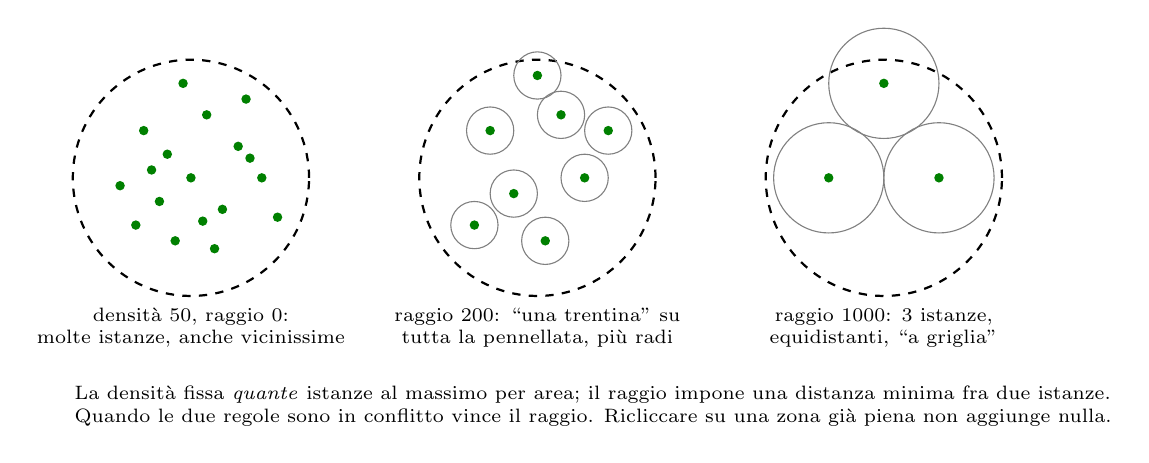
\begin{tikzpicture}[font=\scriptsize, x=1cm, y=1cm]
  % pannello 1: raggio 0
  \draw[thick, dashed] (1.6,1.6) circle (1.5);
  \foreach \p in {(1.0,2.2),(1.3,1.9),(1.8,2.4),(2.2,2.0),(0.7,1.5),(1.2,1.3),(1.6,1.6),(2.0,1.2),(2.5,1.6),(1.4,0.8),(1.9,0.7),(0.9,1.0),(2.3,2.6),(1.5,2.8),(2.7,1.1),(1.1,1.7),(1.75,1.05),(2.35,1.85)}
    {\fill[green!50!black] \p circle (0.06);}
  \node[align=center] at (1.6,-0.3) {densità 50, raggio 0:\\molte istanze, anche vicinissime};
  % pannello 2: raggio medio
  \begin{scope}[xshift=4.4cm]
    \draw[thick, dashed] (1.6,1.6) circle (1.5);
    \foreach \p in {(1.0,2.2),(1.9,2.4),(1.3,1.4),(2.2,1.6),(0.8,1.0),(1.7,0.8),(2.5,2.2),(1.6,2.9)}
      {\fill[green!50!black] \p circle (0.06); \draw[gray] \p circle (0.3);}
    \node[align=center] at (1.6,-0.3) {raggio 200: ``una trentina'' su\\tutta la pennellata, più radi};
  \end{scope}
  % pannello 3: raggio grande
  \begin{scope}[xshift=8.8cm]
    \draw[thick, dashed] (1.6,1.6) circle (1.5);
    \foreach \p in {(0.9,1.6),(2.3,1.6),(1.6,2.8)}
      {\fill[green!50!black] \p circle (0.06); \draw[gray] \p circle (0.7);}
    \node[align=center] at (1.6,-0.3) {raggio 1000: 3 istanze,\\equidistanti, ``a griglia''};
  \end{scope}
  \node[align=left, anchor=west] at (0,-1.3) {La densità fissa \emph{quante} istanze al massimo per area; il raggio impone una distanza minima fra due istanze.\\Quando le due regole sono in conflitto vince il raggio. Ricliccare su una zona già piena non aggiunge nulla.};
\end{tikzpicture}
\caption{Densità e raggio nel Foliage Mode, con i numeri delle prove della lezione. Il
cerchio tratteggiato è il pennello; i cerchi grigi attorno alle istanze rappresentano il
raggio minimo. Ricostruzione schematica: le posizioni dei punti sono indicative.}
\label{ue15:fig:raggio}
\end{figure}

\paragraph{Approfondimento: come piazza il pennello.} Il comportamento visto a lezione è
coerente con il modo in cui il Foliage Mode lavora. A ogni pennellata calcola quante istanze
dovrebbero esserci nell'area del pennello in base a \emph{Density} (istanze per
1000$\times$1000 unità, cioè per 10$\times$10 metri) e alla \emph{Paint Density}; conta quelle
già presenti dello stesso tipo e aggiunge solo le mancanti, scartando ogni posizione
candidata che cada entro il \emph{Radius} di un'istanza esistente. Da qui le tre cose
osservate: ricliccare non aggiunge nulla quando la zona è ``piena''; togliendo il raggio si
riempiono i buchi che il raggio aveva scartato; con un raggio grande la densità teorica non
si raggiunge mai, e le istanze si dispongono a distanza quasi costante. Il raggio è anche il
modo più semplice per evitare alberi compenetrati, il problema che Totten chiama
\emph{casualità percepita} (si veda l'approfondimento della
sezione~\ref{ue15:sec:selezione}). Funzionamento generale dell'engine.

% ---------------------------------------------------------------------
\section{Le altre impostazioni: pendenza, altezza, mobilità, collisioni}
\label{ue15:sec:altre}

\paragraph{Align to Normal e Align Max Angle.} \textbf{Align to Normal} decide se le istanze
``sono allineate alla normal su cui sono applicate''. \textbf{Align Max Angle} è ``quanto si
inclinano per aggiustarsi alla singola pendenza'' (il docente in un primo momento lo confonde
con il parametro successivo e si corregge: ``no, aspetta, mi sa che\dots'').

\paragraph{Ground Slope Angle.} È ``il range in cui il foliage verrà piazzato'': l'angolo
minimo e massimo della superficie su cui un'istanza può comparire. Il docente dipinge l'erba
su un pendio (dopo un momento di confusione: ``stavo modificando ancora le cose dell'albero
invece era l'erba che andava modificata; ci ho cliccato sopra, pensavo di averla selezionata e
invece non era selezionata'', ``è il tipo di cose che vi capiterà sicuramente ogni tanto''). Con
l'intervallo di default, fino a 180, l'erba va ``anche sulla parete rocciosa''. ``Poi sta a voi
decidere se volete che il foliage venga piazzato anche lì oppure no.'' Con un massimo di
\textbf{45} gradi, l'erba compare ``soltanto nelle parti della slope che erano sotto i 47
gradi'' (il docente dice 47 avendo impostato 45: con ogni probabilità è un lapsus), e si
ammucchia nei punti meno ripidi. Abbassando ancora, ``neanche su questa cunetta è stata
messa, perché l'angolazione è troppo alta''. Un uso: mettere attorno alla base del
``montarozzo'' dell'erba a mano, ``per far vedere che un minimo c'è stata un'espansione
erbosa'', senza che salga sulle pareti; ``anche troppo preciso, devo dire''. Il docente lo
rimette a 45 (figura~\ref{ue15:fig:slope}).

\begin{figure}[htbp]
\centering
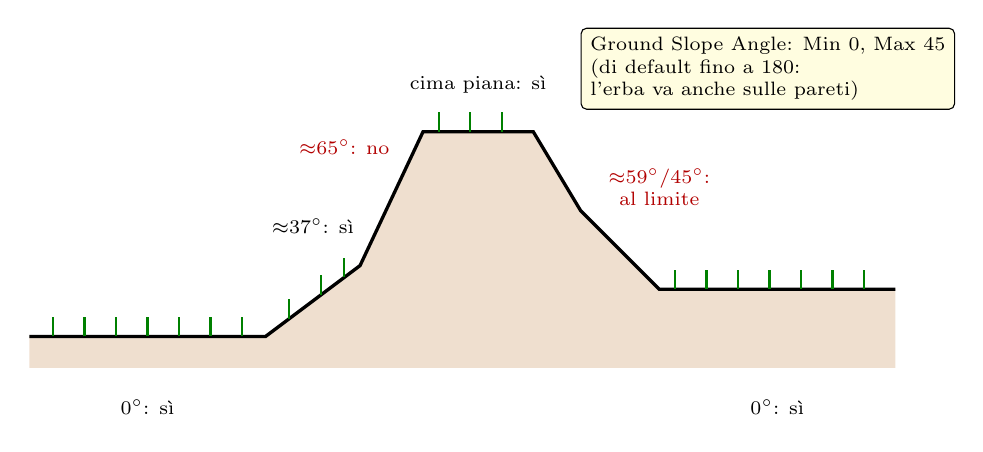
\begin{tikzpicture}[font=\scriptsize, x=1cm, y=1cm]
  \fill[brown!25] (0,0) -- (3,0) -- (4.2,0.9) -- (5.0,2.6) -- (6.4,2.6) -- (7.0,1.6) -- (8.0,0.6) -- (11,0.6) -- (11,-0.4) -- (0,-0.4) -- cycle;
  \draw[very thick] (0,0) -- (3,0) -- (4.2,0.9) -- (5.0,2.6) -- (6.4,2.6) -- (7.0,1.6) -- (8.0,0.6) -- (11,0.6);
  % erba
  \foreach \x in {0.3,0.7,...,2.9} {\draw[green!50!black, thick] (\x,0) -- (\x,0.25);}
  \foreach \x in {3.3,3.7,4.0} {\draw[green!50!black, thick] (\x,{0.75*(\x-3)}) -- (\x,{0.75*(\x-3)+0.25});}
  \foreach \x in {5.2,5.6,...,6.3} {\draw[green!50!black, thick] (\x,2.6) -- (\x,2.85);}
  \foreach \x in {8.2,8.6,...,10.9} {\draw[green!50!black, thick] (\x,0.6) -- (\x,0.85);}
  \node[align=center] at (1.5,-0.9) {0$^\circ$: sì};
  \node[align=center] at (3.6,1.4) {$\approx$37$^\circ$: sì};
  \node[align=center, red!70!black] at (4.0,2.4) {$\approx$65$^\circ$: no};
  \node[align=center] at (5.7,3.2) {cima piana: sì};
  \node[align=center, red!70!black] at (8.0,1.9) {$\approx$59$^\circ$/45$^\circ$:\\al limite};
  \node[align=center] at (9.5,-0.9) {0$^\circ$: sì};
  \node[align=left, anchor=west, draw, rounded corners=2pt, fill=yellow!12] at (7.0,3.4) {Ground Slope Angle: Min 0, Max 45\\(di default fino a 180:\\l'erba va anche sulle pareti)};
\end{tikzpicture}
\caption{Il Ground Slope Angle di un foliage type. Con un massimo di 45 gradi il pennello
piazza istanze solo dove la superficie è inclinata meno di 45 gradi rispetto all'orizzontale;
le pareti restano spoglie. Gli angoli indicati sono esempi. Ricostruzione schematica.}
\label{ue15:fig:slope}
\end{figure}

\paragraph{Height.} Il range d'altezza in cui il foliage può essere piazzato. Di default va
da meno a più infinito (``da meno a più''); con \textbf{0 -- 10}, ``appena andiamo sopra i 10
d'altezza, lui smette di piazzarla''.

\paragraph{Mobility.} Come per le luci: \textbf{Static}, ``più veloci da renderizzare'', che
``funzionano col baking'', o \textbf{Movable}, ``completamente dinamiche'', con le luci che
``reagiscono in tempo reale'', ``ma è più lento da gestire''.

\paragraph{Cull Distance.} ``La distanza massima da cui non smettono di essere renderizzate.''
Allontanandosi, ``tutto il resto del foliage è sparito'', quello del materiale, ``ma questo è
rimasto, perché c'è zero di cull distance'': ``non ha massimo e minimo, esiste e basta, non viene
tagliato, è sempre renderizzato''. ``Gestitelo sulla base della grandezza della vostra scena.''

\paragraph{Le ombre e il dressing.} \emph{Cast Shadow}, ombre dinamiche e statiche,
\emph{Affect Dynamic Lighting}: ``tutti i check che potete gestirvi per la resa estetica con
la luce''. L'erba del pacchetto ``è fatta apposta per non castare ombre''. Il foliage si può
dipingere anche \emph{sopra} le mesh: il docente mette dell'erba sopra una struttura della
base, e immagina ``un mondo post apocalittico con una pompa di benzina abbandonata'' (``non so
perché mi ha fatto pensare alla pompa di benzina''), con l'erba che ci cresce sopra e ``dei
\emph{vine} che scendono giù'' (delle liane, dei rampicanti).

\paragraph{Collision Presets.} ``E poi abbiamo i preset delle collisioni.'' La frase del docente
è ambigua (``di default tutto il foliage è impostato a una collisione, che nel caso dell'erba
ci fa anche comodo, perché noi non vogliamo che ci sia l'erba e poi ci inciampiamo sopra''):
il senso è che \emph{per l'erba} si vuole che non ci siano collisioni. ``Quando andiamo a
mettere gli alberi, però, dobbiamo assicurarci che lì sia tutto funzionale, che le collisioni
ci siano, perché altrimenti possiamo passarci attraverso.''

\paragraph{L'ingresso della base.} Prima degli alberi il docente sistema l'erba davanti alla
base: ``il nostro personaggio uscirà da lì e si trova prima l'erbetta che va a gradiente, poi
c'è il folto''.

\paragraph{Approfondimento: le impostazioni del foliage type.} Qualche precisazione sui
parametri visti. \emph{Ground Slope Angle} confronta la normale della superficie con la
verticale, come il World Aligned Blend dell'automaterial: le due cose si possono far
coincidere, così che il foliage manuale non finisca dove il materiale mette la roccia.
\emph{Height} usa la quota assoluta del mondo in centimetri, quindi ``0 -- 10'' è una fascia di
dieci centimetri sopra lo zero del mondo, utile per esempio per non piantare canne sopra il
livello dell'acqua. \emph{Cull Distance} ha un minimo e un massimo: fra i due le istanze
sfumano, e con entrambi a 0 il culling per distanza è disattivato, come visto. I
\emph{Collision Presets} del foliage type (\emph{Body Instance}) decidono come le istanze
\emph{rispondono} alle collisioni; perché ci sia una collisione, però, la mesh deve averne una
(la sezione successiva lo mostra). Romero e Sewell descrivono nel capitolo 14 (``Math and
Trace Nodes'') la tabella delle \emph{Collision Responses}: ogni oggetto ha un \emph{Object
Type} e una risposta (\emph{Ignore}, \emph{Overlap} o \emph{Block}) per ogni canale, con dei
preset come \emph{BlockAll}, \emph{OverlapAllDynamic} e \emph{Pawn}, oppure
\emph{Custom\ldots}; nel capitolo 5 impostano \emph{BlockAllDynamic} su un oggetto
interattivo. Le stesse regole valgono per le istanze del foliage.

% ---------------------------------------------------------------------
\section{Gli alberi e le collisioni}
\label{ue15:sec:alberi}

\paragraph{Le impostazioni dell'albero.} ``Togliamo l'erba, perché sennò dipingiamo anche
l'erba insieme agli alberi.'' Le impostazioni del pacchetto: \textbf{Density 1}, ``abbastanza
sparsi'', raggio 0: ``ci può stare''. Il docente ne mette una fila all'ingresso, ``una piccola
radura''. Gli alberi sono di taglie diverse (\textbf{Scale} da 1 a 3: ``con l'albero funziona
meglio, dà un'idea migliore''; c'è l'albero ``di base'' e ``l'albero grosso'') e ruotati in
maniera diversa: lo Z Offset è 0, ma c'è il \textbf{Random Yaw}, ``una rotazione randomica
sull'asse verticale''. Togliendolo, ``gli alberi vanno tutti nella stessa direzione, sono tutti
curvi in quella direzione, verso sinistra''; rimettendolo, ``iniziano a ruotare''. (Un albero
``si è rifiutato di essere cancellato''.)

\paragraph{Alberi dalle pareti.} Lasciando il Ground Slope Angle ampio e Align to Normal
attivo, si possono piantare alberi su una parete: ``alberi che escono dalle pareti, non so
perché dovreste volerlo fare, ma lo potete fare''. Per esempio ``un percorso di alberi tutto
attaccato sul lato della parete, che potete utilizzare come percorso per un platform''.
Togliendo Align to Normal ``ve li spawna dritti''. Con gli alberi l'allineamento ``non funziona
granché bene'', ``ma per esempio con dei cespugli o dei funghi parassiti'' sì.

\paragraph{La collisione strana.} Le collisioni dell'albero sono \textbf{Block All}. ``Col
nostro robottino andiamo all'avventura'': ``siamo alti quanto l'erba'' (bisognerà abbassarla).
In Play si riesce a passare dentro gli alberi, almeno in parte: ``hanno una strana
collisione''. Prima di guardare, il docente chiarisce ``una grossa cosa'' sulle collisioni:
``questo parametro non determina se l'oggetto avrà collisioni o meno; determina se le
collisioni dell'oggetto sono attive o meno, e per cosa sono attive''. La prova: Block All
sull'\textbf{erba}. ``Sono positivamente sicuro che potremo comunque camminare dentro l'erba'':
ed è così (``se dovessimo esplorare un open world del genere, il nostro personaggio dovrebbe
muoversi più veloce di così''). Il motivo è nella static mesh di base: nello Static Mesh
Editor, con \textbf{Show Simple Collision}, ``non ci sono simple collision, quindi non c'è
nulla da attivare''. ``Vi capiterà di mettere degli asset in scena, iniziare a giocare e
passarci attraverso, perché magari quegli asset sono stati importati o esportati senza le
collisioni''; e anche impostando ``le collisioni che bloccano tutto, o che bloccano solo i
proiettili'', ``lui comunque non può bloccare, perché non c'è nulla da bloccare''.

\paragraph{L'albero, dentro.} Aprendo la mesh dell'albero: ``ah, geniale. L'hanno messa dalla
parte sbagliata.'' Le forme della collisione semplice (``diversi pezzi'') sono ruotate rispetto
al tronco, ``credo che l'abbiano importato proprio con la collisione sbagliata''. Si possono
selezionare tutte e ruotare ``dalla parte corretta''; ``anche se sono proprio strane'',
sbagliate anche nelle proporzioni. Tre strade:
\begin{enumerate}
  \item \textbf{ruotare} le forme esistenti, come fa il docente (``tanto il nostro giocatore
        non andrà mai a collidere lassù, a meno che non vogliamo che lo faccia'');
  \item \textbf{eliminare} le simple collision e scegliere \textbf{Use Complex Collision As
        Simple}: la collisione prende ``esattamente i poligoni dell'albero''. ``Chiaramente
        questa cosa è pesante, però vi risolve il problema di dover fare le collisioni a
        mano'';
  \item \textbf{rifarle} a mano con forme semplici: ``vi basterebbe prendere un cilindro,
        metterlo in diagonale, e qui sopra metterci un piano circolare''. Il docente aggiunge
        una \textbf{capsula}, la fa più piccola e più stretta, la ruota lungo il tronco, e
        sopra una \textbf{box piatta}, ``in modo che il giocatore possa salire sulla cima
        dell'albero e rimanerci sopra'' (figura~\ref{ue15:fig:collisione}).
\end{enumerate}
Se si vuole che il personaggio salti da un albero all'altro o percorra la parete passando sui
tronchi, ``non potete fare questa cosa'' con la collisione originale: ``dovete togliere queste
collisioni e rifarle''.

\begin{figure}[htbp]
\centering
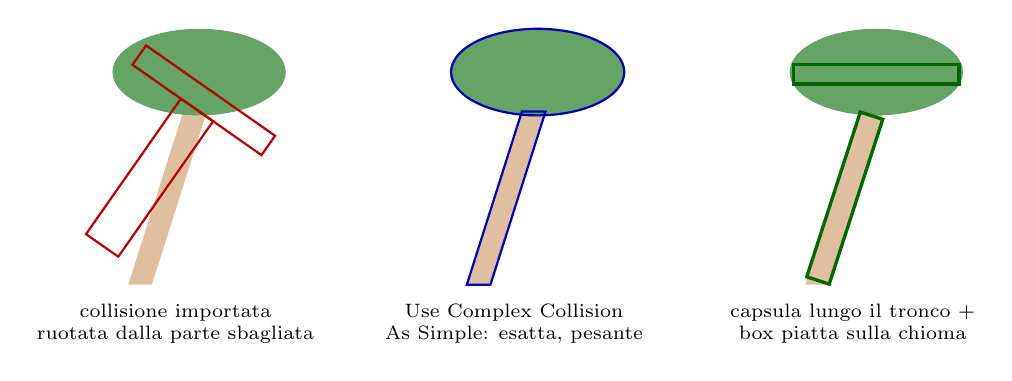
\begin{tikzpicture}[font=\scriptsize, x=1cm, y=1cm]
  % albero originale
  \begin{scope}
    \fill[brown!50] (0.9,0) -- (1.2,0) -- (1.9,2.2) -- (1.6,2.2) -- cycle;
    \fill[green!40!black!60] (1.8,2.7) ellipse (1.1 and 0.55);
    \draw[red!70!black, thick, rotate around={-35:(1.2,1.4)}] (0.95,0.3) rectangle (1.45,2.4);
    \draw[red!70!black, thick, rotate around={-35:(1.2,1.4)}] (0.2,2.4) rectangle (2.2,2.7);
    \node[align=center] at (1.5,-0.5) {collisione importata\\ruotata dalla parte sbagliata};
  \end{scope}
  % complex as simple
  \begin{scope}[xshift=4.3cm]
    \fill[brown!50] (0.9,0) -- (1.2,0) -- (1.9,2.2) -- (1.6,2.2) -- cycle;
    \fill[green!40!black!60] (1.8,2.7) ellipse (1.1 and 0.55);
    \draw[blue!70!black, thick] (0.9,0) -- (1.2,0) -- (1.9,2.2) -- (1.6,2.2) -- cycle;
    \draw[blue!70!black, thick] (1.8,2.7) ellipse (1.1 and 0.55);
    \node[align=center] at (1.5,-0.5) {Use Complex Collision\\As Simple: esatta, pesante};
  \end{scope}
  % capsula + box
  \begin{scope}[xshift=8.6cm]
    \fill[brown!50] (0.9,0) -- (1.2,0) -- (1.9,2.2) -- (1.6,2.2) -- cycle;
    \fill[green!40!black!60] (1.8,2.7) ellipse (1.1 and 0.55);
    \draw[green!40!black, very thick, rotate around={-18:(1.4,1.1)}] (1.25,0.0) rectangle (1.55,2.2);
    \draw[green!40!black, very thick] (0.75,2.55) rectangle (2.85,2.8);
    \node[align=center] at (1.5,-0.5) {capsula lungo il tronco +\\box piatta sulla chioma};
  \end{scope}
\end{tikzpicture}
\caption{Tre modi di sistemare la collisione dell'albero di StackOBot visti a lezione:
ruotare le forme importate male, usare la geometria della mesh come collisione, oppure
rifare la collisione con una capsula (qui disegnata come un rettangolo inclinato) e una box
piatta su cui il giocatore può stare in piedi. Ricostruzione schematica.}
\label{ue15:fig:collisione}
\end{figure}

\paragraph{La domanda sulle collisioni a senso unico.} Uno studente ha una domanda ``fuori
tema'': ``le collisioni che funzionano da un solo lato?'' Gli è venuto in mente un gioco (``PIC''
nella trascrizione: con ogni probabilità \emph{PEAK}, il gioco cooperativo di arrampicata, ma
il nome non è certo) in cui ``puoi salire sugli alberi e puoi attraversare le foglie da sotto,
ma non puoi attraversarle da sopra''. Il docente non ci ha mai pensato: ``probabilmente dipende
dal modo in cui è codificato quel tipo di interazione''. ``Gli dici che se stai andando in una
direzione non deve contare quella collisione, se stai andando nell'altra deve contarla.
Penso, non lo so, a naso direi che è questo.'' Non ha giocato il gioco.

\paragraph{No Collision sovrascrive.} Rimesso tutto com'era, con le collisioni girate ``dalla
parte giusta'', il docente imposta \textbf{No Collision} nel foliage type dell'albero: ``lui
sovrascrive il fatto che ha delle collisioni''. In Play ci si passa attraverso, ``perché l'asset
del foliage non ha collisioni''. Con \textbf{Custom} si sceglie che cosa bloccano: ``se bloccano
la camera, se bloccano i proiettili, se bloccano il pawn''. ``Di base, il Block All andrà
bene.''

\paragraph{Approfondimento: collisione semplice, complessa e a senso unico.} Una static mesh
ha due rappresentazioni di collisione. La \emph{simple collision} è fatta di primitive
(box, sfere, capsule, convessi) ed è quella usata dalla fisica e dal movimento del
personaggio: è economica, ma va costruita (nello Static Mesh Editor, menu
\emph{Collision}: \emph{Add Box}, \emph{Add Capsule}, \emph{Auto Convex Collision}\dots)
o importata dal programma di modellazione. La \emph{complex collision} è la mesh stessa,
triangolo per triangolo, usata di solito solo per le tracce precise. \emph{Collision
Complexity: Use Complex Collision As Simple} fa usare la seconda anche per la fisica: comoda,
ma costosa su mesh dense e, per i corpi simulati, non utilizzabile. Le collisioni ``a senso
unico'' delle piattaforme attraversabili da sotto non sono una proprietà della collisione
in Unreal: si ottengono via codice, per esempio con un volume sotto la piattaforma che, quando
il personaggio sale, gli fa ignorare il canale della piattaforma (\emph{Ignore}) e lo
ripristina quando il personaggio è sopra, oppure controllando la velocità verticale; è
proprio la risposta ``a naso'' del docente. Le risposte \emph{Ignore}/\emph{Overlap}/\emph{Block}
per canale sono quelle della tabella del capitolo 14 di Romero e Sewell; il resto è
funzionamento generale dell'engine.

% ---------------------------------------------------------------------
\section{Selezionare, rifinire e il foliage non naturale}
\label{ue15:sec:selezione}

\paragraph{Il cespuglio a mano.} ``Lo stesso con gli altri oggetti.'' Il cespuglio del
pacchetto spawna poco; è ``un tipo di asset che io, piuttosto che metterlo così, farei
\textbf{single} e andrei a posizionare a mano'': ``voglio che queste cose stiano molto
ammucchiate vicino agli alberi''. Le dimensioni sono comunque casuali, ``forse troppo varie
per i miei gusti''. Allo stesso modo si fa ``un percorso alberato'', con alberi a destra e a
sinistra, che ``fa comunque parte del foliage'' e si integra con il resto.

\paragraph{Gli strumenti di selezione.}
\begin{itemize}
  \item \textbf{Select}: si prende ``il singolo pezzo di foliage'' e lo si sposta (``no, no,
        quest'albero non deve stare proprio lì, deve stare qui''), ``un po' tipo selection mode,
        ma con tutti gli asset che rimangono all'interno del foliage''. Tornando in Selection
        Mode e cliccando, invece, si seleziona tutto il foliage actor. (Il docente trova
        nell'Outliner anche delle istanze che non si aspettava, ``saranno delle cose che
        c'erano prima'', e non approfondisce.)
  \item \textbf{Select All} e \textbf{Deselect}: tutte le istanze dei tipi attivi, da
        muovere insieme.
  \item \textbf{Select Invalid}: ``mi porta automaticamente alle instance che sono invalide,
        quindi quelle che vanno modificate''.
  \item \textbf{Lasso}: ``funziona un po' tipo Photoshop'': invece di cliccare, si evidenzia
        una zona. Vale solo per i tipi spuntati: ``qui ci sono sempre attivi soltanto gli
        alberi, quindi se voglio fare questa cosa devo prendere anche questi''.
  \item \textbf{Remove}: ``questi alberi qua non mi piacciono'': elimina tutto ciò che è stato
        evidenziato.
  \item un ultimo strumento, ``stessa cosa con i raise, però è un discorso un po' diverso, poi
        modifica piano piano'': il nome non è ricostruibile con certezza (con ogni probabilità
        \emph{Reapply}, che riapplica le impostazioni del foliage type alle istanze già
        dipinte).
\end{itemize}

\paragraph{Non deve essere naturale.} ``È tendenzialmente uno strumento che utilizzate
principalmente per motivi estetici.'' E ``non deve essere necessariamente naturale'': si può
usare ``con ogni mesh che voglio''. ``Se io voglio riempire la scena di robottini, lo posso
fare''; una scena in metropolitana con il pavimento pieno di ``cartacce, plastiche, cose
varie''. ``È un po' un pennello con cui piazzare rapidamente tutta una serie di oggetti.''

\paragraph{Le rocce sotto lo zero.} Le rocce dipinte ``appena si avvicinano allo zero
impazziscono; invece sopra sono perfette''. Consiglio: ``mettete il piano di base leggermente
più alto dello zero''. Spostando una roccia, il materiale cambia: ``cambia sulla base
dell'altezza''; ruotandola, ``così diventa una parete rocciosa''. ``È un po' strano che abbiano
scelto di fare un materiale dinamico così per un oggetto standard.'' Aprendo il materiale
(``più complesso di quello che pensavo''), il docente legge nomi come \emph{Virtual
Texture}, \emph{World Position} e una ``variation'' (la trascrizione dice ``part time, drop
variation'', non ricostruibile): ``hanno provato a fare una roba carina'' per avere un
materiale dinamico, ``tipo il \textbf{vertex painting}'', e per ``blendare la mesh con
l'oggetto del landscape'' quando si dipinge il materiale del landscape. Ma ``volendo, potete
fare anche letteralmente solo una texture di roccia'' con le sue mappe, ``e avete comunque una
roccia''.

\paragraph{Approfondimento: la casualità percepita.} Il Foliage Mode rende facilissimo
spargere oggetti a caso, ed è proprio il rischio che Totten descrive nel capitolo 8
(``Possibility Spaces and Worldbuilding''): in natura alberi, rocce e scogliere si dispongono
nel tempo in modi non pianificati, e i designer alle prime armi piazzano alberi, rocce ``e
perfino edifici'' a caso sulla mappa, ``ignari dell'importanza della loro posizione''; il
risultato è una \emph{casualità percepita} che non dice nulla al giocatore. ``Dirigere lo
sguardo verso elementi scenici piazzati con cura'' è il modo in cui il giocatore capisce il
mondo. In pratica: il pennello per la massa (l'erba, il bosco di sfondo), lo \emph{Single
Instance Mode} e il \emph{Select} per gli elementi che contano (l'albero isolato che fa da
landmark, i cespugli che incorniciano un passaggio), che è esattamente il modo di lavorare del
docente con i cespugli. Nel capitolo 3 (``Basic Gamespaces'') Totten aggiunge che un cambio
nel tipo di vegetazione segnala il passaggio a una zona nuova, come un cambio di texture sul
terreno. Sul materiale delle rocce: un materiale che campiona texture in world space
(\emph{world aligned}) cambia aspetto quando l'oggetto si sposta o ruota, perché la texture
resta ferma nel mondo mentre la mesh si muove; e un calcolo basato sulla quota assoluta (per
esempio per sfumare la base nella sabbia o nell'umidità) produce effetti strani sotto lo
zero, se chi l'ha fatto ha supposto che il terreno stia sopra. Funzionamento generale
dell'engine; il grafo del materiale non è stato verificato nel capitolo.

% ---------------------------------------------------------------------
\section{La domanda sui mondi procedurali}
\label{ue15:sec:procedurale}

\paragraph{Landscape o mesh?} ``Ci sono domande?'' Uno studente: ``i mondi che si generano
automaticamente usano il landscape o le mesh?'' ``Tipo le robe procedurali? Tendenzialmente
dipende.'' ``È più comodo farlo con le mesh, perché puoi farti un \textbf{array} di oggetti e
puoi piazzarli secondo dei criteri che hai scelto tu.'' Ma ``l'ultima volta che ho lavorato
con qualcosa di procedurale era un sacco di tempo fa'', e magari ci sono ``nuovi nodi'' o
``feature che Unreal ha inserito'' che il docente non conosce. Il consiglio: cercare sullo store
``qualche pacchetto che parla di asset procedurali, non modulari, proprio procedurali, che ha
dei sistemi di proceduralizzazione'', e ``ti studi un po' loro come le fanno''. ``Fab, intendi,
giusto?'' ``Sì, su Fab. Ai miei tempi non si chiamava Fab, mi sento vecchio.''

\paragraph{Lo strumento che non si trova.} Parlando di procedurale, il docente ricorda ``un
tool che io non ho mai usato, che dovrebbe essere relativamente nuovo'': ``una specie di box
all'interno della quale possono essere impostati dei parametri, e spostando questa box e
ingrandendola, lui va a piazzare quel tipo di foliage nel volume che c'è all'interno''. Lo
cerca fra i tipi di asset del menu \emph{Foliage} (c'è lo \emph{Static Mesh Foliage}, ``questo
qui è letteralmente il nuovo, ma non è quello che voglio''), non lo trova, e ipotizza che
fosse ``un plugin''. ``Me lo devo vedere meglio.''

\paragraph{Sprite e flipbook.} Nello stesso menu ``vi potete vedere tutti i tipi di asset che
possono essere creati'', anche gli \textbf{sprite} e i \textbf{flipbook}: ``carini se volete
fare, che ne so, un menu animato''. ``Visto che avete fatto la roba col menu, con un flipbook
potete andare a fare l'animazione del menu.''

\paragraph{Approfondimento: generazione procedurale in Unreal.} Lo strumento descritto dal
docente corrisponde con ogni probabilità a uno di due sistemi, ed entrambi si attivano da
plugin. Il primo è il \emph{Procedural Foliage Spawner} con il suo \emph{Procedural Foliage
Volume}: si definisce quali foliage type crescono, con quali regole di competizione e di
età, e si fa ``simulare'' la crescita dentro il volume (è una funzione sperimentale,
\emph{Procedural Foliage}, da abilitare nelle impostazioni dell'editor). Il secondo, più
recente e oggi il sistema di riferimento, è il framework \emph{PCG} (\emph{Procedural
Content Generation}), con il \emph{PCG Volume} e un grafo a nodi che campiona superfici,
filtra i punti per pendenza o altezza e vi genera mesh: il plugin si chiama
\emph{Procedural Content Generation Framework}. La risposta del docente sulle mesh resta
valida: anche il PCG, alla fine, produce istanze di static mesh. Romero e Sewell, nel
capitolo 19 (``Procedural Generation''), definiscono la generazione procedurale come ``un
metodo per creare il contenuto del livello usando script invece che a mano'', utile per
evitare compiti ripetitivi; la costruiscono con il \emph{Construction Script}, un
\emph{Instanced Static Mesh Component} e dei cicli \emph{For Loop} che dispongono righe di
istanze, e poi con le \emph{Blueprint Spline} per piazzare actor lungo un percorso. Gli
sprite e i flipbook appartengono a \emph{Paper2D}, il sistema 2D dell'engine: un flipbook è
una sequenza di sprite riprodotta a una certa velocità. Fab è lo store di Epic che dal 2024
ha sostituito l'Unreal Engine Marketplace, quello usato nel capitolo 9 del libro per
importare l'\emph{Animation Starter Pack}.

% ---------------------------------------------------------------------
\section{Il Niagara e il Post Process Volume}
\label{ue15:sec:postprocess}

``Come ho detto, ci abbiamo una decina di minuti.'' In quella decina di minuti si potrebbe
``buttare un occhio'' sul post process, ``visto che ci siamo''.

\paragraph{Un'occhiata al Niagara.} Prima, ``al volo'', il Niagara: ``è proprio un editor a
parte''. Creando un \textbf{Niagara System} si sceglie fra ``tutte le varie forme, modi, colori,
possibilità'' dei \emph{preset}; il docente prende una \textbf{Fountain}, ``la base della
cosa''. Dentro c'è ``tutto un sistema così, con la timeline, con degli \textbf{emitter}, tutte
cose''. ``È una roba un po' complicata, magari ce la vediamo alla prossima lezione se
riusciamo.''

\paragraph{Dove si trova il post process.} Dal \textbf{Place Actors}, nella categoria
\textbf{Volumes}, ``tra le varie cose'' (``insieme a tutta una serie di altre cose molto, molto
carine'') c'è il \textbf{Post Process Volume}: ``il nostro quadratone''.

\paragraph{Che cos'è.} ``È un volume all'interno del quale voi andate ad applicare delle
modifiche alla lente della telecamera, fondamentalmente.'' ``Voi andate a modificare il modo in
cui le cose appaiono, non il modo in cui le cose sono.'' Le stesse ``lenti'' esistono anche su
una \textbf{Camera Actor}: nei suoi Details, nella sezione \emph{Post Process}, ``abbiamo
diverse lenti che possiamo andare a modificare'', e queste modifiche ``si applicano solo alla
singola telecamera''. Il volume invece applica gli effetti \emph{al suo interno}.

\paragraph{Le transizioni.} ``Vi siete mai chiesti come fanno a fare quegli effetti per cui
quando entri o esci da una casa il bloom della luce è particolarmente forte e poi si attenua?
O com'è possibile che la luce fuori era molto forte, io entro dentro una grotta e piano piano
la luce diventa più tenue e cambia colore?'' ``È perché il post process ha degli effetti di
transizione fra l'interno e l'esterno.'' Si possono piazzare più Post Process Volume con
effetti diversi, e passando dall'uno all'altro cambia ``il modo in cui la mia telecamera va a
gestire le cose''.

\paragraph{I volumi annidati.} Si può anche mettere un post process dentro un altro, ``una roba
complicata che vi sconsiglierei di fare'': il volume interno ``calcola tutto quello che lui
deve calcolare e in più ci applica anche quello'' dell'esterno. L'esempio: il volume interno
rende la scena gialla (\emph{color correction}), quello esterno blu; stando nell'interno ``vediamo
tutto verde, perché lui somma la color correction dei due post process''. ``Per cui diventa molto
complicato capire cosa vogliamo fare.'' (Figura~\ref{ue15:fig:postprocess}.)

\paragraph{Un solo volume per tutto: Infinite Extent.} ``Se voglio un unico post process che
determina il modo in cui la scena viene vista, devo renderlo incredibilmente grande?'' No:
nei Details del volume (``le stesse lenti che aveva il camera actor, con qualche opzione in
più'') si cerca \emph{infinite} e si trova \textbf{Infinite Extent (Unbound)}: ``quando questa
casella viene spuntata, il volume copre tutto il mondo, non solo l'area all'interno'', e i
cambiamenti ``vengono visti allo stesso modo in tutta la zona''. Per ora la si toglie.

\paragraph{Le lenti, per la prossima volta.} ``Non so quanto senso abbia iniziare a parlare
delle lenti: ci abbiamo 5 minuti, e ogni lente ha un sacco di parametri.'' Due accenni: il
\textbf{Bloom}, ``abbastanza semplice'', ``quello che serve per i god shaft'' di cui si parlava
prima; e la \textbf{Chromatic Aberration}: ``occhio, che fa male agli occhi''. Il resto alla
prossima lezione.

\begin{figure}[htbp]
\centering
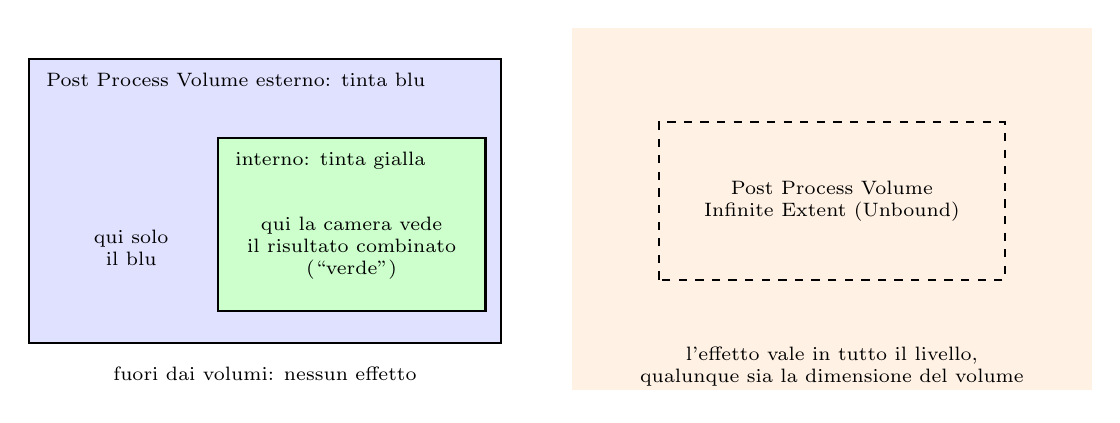
\begin{tikzpicture}[font=\scriptsize, x=1cm, y=1cm]
  \draw[thick, fill=blue!12] (0,0) rectangle (6,3.6);
  \node[anchor=north west] at (0.1,3.55) {Post Process Volume esterno: tinta blu};
  \draw[thick, fill=green!20] (2.4,0.4) rectangle (5.8,2.6);
  \node[anchor=north west, align=left] at (2.5,2.55) {interno: tinta gialla};
  \node[align=center] at (4.1,1.2) {qui la camera vede\\il risultato combinato\\(``verde'')};
  \node[align=center] at (1.3,1.2) {qui solo\\il blu};
  \node[align=center] at (3,-0.4) {fuori dai volumi: nessun effetto};
  % unbound
  \begin{scope}[xshift=7.2cm]
    \fill[orange!10] (-0.3,-0.6) rectangle (6.3,4.0);
    \draw[thick, dashed] (0.8,0.8) rectangle (5.2,2.8);
    \node[align=center] at (3,1.8) {Post Process Volume\\Infinite Extent (Unbound)};
    \node[align=center] at (3,-0.3) {l'effetto vale in tutto il livello,\\qualunque sia la dimensione del volume};
  \end{scope}
\end{tikzpicture}
\caption{A sinistra, due Post Process Volume annidati: dentro il volume interno la camera
riceve l'effetto di entrambi, come nell'esempio del docente (giallo e blu che danno verde). A
destra, un volume con \emph{Infinite Extent (Unbound)}, che vale per tutto il livello.
Ricostruzione schematica.}
\label{ue15:fig:postprocess}
\end{figure}

\paragraph{Approfondimento: come si combinano i post process.} Il comportamento dei volumi
sovrapposti è un po' più ordinato della ``somma'' descritta a lezione. Ogni Post Process
Volume ha una \emph{Priority}, un \emph{Blend Weight} (da 0 a 1) e un \emph{Blend Radius}, la
distanza dal bordo entro cui l'effetto sfuma: è il Blend Radius che produce le transizioni
graduali fra esterno e grotta. Ogni volume modifica solo le proprietà la cui casella è
spuntata; quando la camera è dentro più volumi, Unreal li applica in ordine di priorità, e
per ogni proprietà il valore del volume a priorità più alta si \emph{mescola} con quello già
calcolato secondo il suo Blend Weight (con peso 1 lo sostituisce). Se due volumi cambiano
proprietà diverse, si vedono entrambe le modifiche; se cambiano la stessa con peso minore di
1, si ottiene una via di mezzo: in questo senso le due tinte possono dare un colore
combinato. Il consiglio del docente resta buono: pochi volumi, priorità esplicite, e di solito
un volume \emph{Unbound} a priorità bassa per l'aspetto generale del livello più volumi locali
per le zone speciali. Le impostazioni della Camera Actor (e del \emph{Camera Component} del
personaggio) si combinano con quelle dei volumi, con un proprio peso. Romero e Sewell, nel
capitolo 9 (``Building Smart Enemies with Artificial Intelligence''), allargando l'area di
gioco ricordano che il \emph{PostProcessVolume} e il \emph{LightmassImportanceVolume} ``devono
coprire la nuova area di gioco'', perché ``questi volumi sono usati per l'illuminazione e gli
effetti''; nel capitolo 12 indicano la qualità del \emph{Post Processing} (filtri come motion
blur e bloom applicati allo schermo dopo il rendering della scena) fra le impostazioni da
ridurre se le prestazioni sono basse. Il resto è funzionamento generale dell'engine.

% ---------------------------------------------------------------------
\section{I compiti, la vetrata colorata e la chiusura}
\label{ue15:sec:chiusura}

\paragraph{Il compito.} ``Visto che le cose principali che abbiamo visto in queste due lezioni
sono sicuramente il landscape e sicuramente il foliage'', il compito per il fine settimana,
``come abbiamo fatto settimana scorsa con la gym e il livello'':
\begin{itemize}
  \item in un altro livello, o nello stesso, ``un piccolo spazio'': un piccolo landscape con
        il suo foliage, ``che abbia un'estetica abbastanza curata'' (``gli oggetti che avete a
        disposizione sono pochi, quindi non potete fare troppa roba'');
  \item che \textbf{circondi la vostra gym}, ``il posto in cui avete messo le cose'', e in cui
        il personaggio ``possa muoversi un po', girovagare''; conviene aumentare un po' la
        velocità di movimento del personaggio;
  \item lo scopo: ``un piccolo livellino di \textbf{esplorazione} utilizzando il landscape''.
        ``Nulla di troppo complesso'': magari ``delle pedane che vi fanno salire e scendere da
        una parte all'altra''; come la volta scorsa, ``un paio di \textbf{collezionabili} in
        giro''; ``delle alture, degli avvallamenti'', e ``se ve la sentite particolarmente
        creativi, anche dei buchi, delle grotticine'';
  \item ``potete mettere in pratica il fatto di dover saltare sugli alberi, se volete'':
        sistemate le collisioni e via.
\end{itemize}
(Nel mostrarlo, il docente alza un pezzo di terreno e ``clippa'' tutto: ``adesso sono sul
cane'', cioè, con ogni probabilità, sotto o dentro la geometria; ``siamo direttamente sulla
sabbia''.)

\paragraph{Le dimensioni.} ``Chiaramente non deve essere una mappa così grande.'' Il docente
ragiona ad alta voce: ``15 per 15 va piccolino'', ``\textbf{31 per 31} conviene, che avete
abbastanza spazio per fare un po' di cose''. (La trascrizione non dice a che cosa si
riferisca il numero; 31 per 31 è uno dei valori della \emph{Section Size} visti nella lezione
precedente, ma potrebbe anche indicare il numero di quad del landscape. In ogni caso il
senso è: un landscape piccolo.) Si può usare il materiale costruito insieme e ``sbizzarrirsi
un pochino'', ``costruire qualcosina''.

\paragraph{Il video.} ``Se volete potete anche mettere un video di voi che camminate in
quell'ambiente su Discord'': si registra e lo si carica. Uno studente che non ci sarà
all'ultima lezione: ``io penso che farò così''. ``Va benissimo: è comunque una testimonianza del
fatto che fate cose. Magari ispirate gli altri.'' Vale anche per i livelli e le gym della
volta scorsa. ``Fateli poco pesanti però, perché Discord mi sa che non vi permette di caricare
troppa roba''; altrimenti si mettono su un Drive e si condivide il link.

\paragraph{La domanda sul volume.} Lo studente che mancherà all'ultima lezione chiede del post
process: ``la lente funziona nel momento in cui stai dentro l'area, o funziona attraverso, se
guardi attraverso?'' ``Dentro'': ``è un volume, è come un trigger volume, come un blocking
volume; funziona nel momento in cui tu sei all'interno del volume''. Se si vuole una stanza di
un colore, ``devi mettere il post process tutto attorno all'ambiente''.

\paragraph{La vetrata colorata.} ``Ma quindi, per esempio, una finestra colorata che trasforma
la luce in luce colorata usa le lenti o qualcos'altro?'' ``Usa un po' di entrambi,
tendenzialmente. Quando ti fai questa domanda, la risposta è sempre: entrambi.'' L'esempio è la
\textbf{vetrata di una chiesa}:
\begin{enumerate}
  \item un oggetto con un \textbf{materiale di vetro}, ``che permetta di vedere attraverso'' e
        ``del giusto colore per dare quell'idea'';
  \item una \textbf{luce forte} proiettata attraverso, con il colore cambiato ``in modo che la
        luce sia di quel colore lì'';
  \item il \textbf{post process} ``per accentuare l'effetto di cambio della luce''.
\end{enumerate}
E se la directional light deve restare bianca, vista da fuori, ma colorata da dentro? Allora
``senza cambiare la luce'': il materiale del vetro ``che comunque filtra un pochino la luce'', e
il post process che, mentre sei dentro, cambia il colore percepito. ``Ah, è una specie di
escamotage.'' ``È tutto un escamotage.'' ``Costruire livelli diventa sempre tipo trovare il
\textbf{trucchetto del mago} per ingannare la persona.'' Si potrebbe certo fare in modo che
``nel momento in cui la luce attraversa quel determinato trigger il calcolo del colore della
luce cambi'', ``però è sicuramente più complicato e più dispendioso che fare un trucchetto''.

\paragraph{La chiusura.} Domande e lavori si possono mettere sul Discord. ``La prossima lezione,
sicuramente, vi parlo al volo del \textbf{packaging}'': ``così, oltre a fare il video, magari
possiamo proprio fare un eseguibile che può essere passato e può essere giocato anche dagli
altri''. ``Buon fine settimana, buona serata. E ci vediamo martedì prossimo.''

\paragraph{Approfondimento: la luce attraverso il vetro.} In Unreal Engine~5 una luce non
cambia colore da sola attraversando un materiale traslucido: le ombre dei materiali
\emph{translucent} sono di norma solo più o meno scure, non colorate. Per questo il ``trucco del
mago'' del docente è la strada pratica: una \emph{spot light} o una \emph{rect light} colorata
dietro la vetrata, eventualmente con una \emph{Light Function} (un materiale che maschera la
luce con il disegno della vetrata) per proiettare il motivo sul pavimento, un cono finto come
quelli dell'engine per il fascio, e un Post Process Volume nella navata per la tinta
generale. Totten, nel capitolo 5 (``Introducing Emotional Level Design through Survival
Instincts''), parla proprio di questa luce: l'\emph{ombra} (\emph{shade}) ottenuta facendo
entrare luce diffusa attraverso tende, schermi o vetrate fu un tratto centrale
dell'architettura gotica, che cercava un'esperienza eterea chiamata \emph{lux nova}, ``luce
nuova'' o ``luce mistica''; e la stessa condizione, con la nebbia, è un caposaldo dell'horror.
Nel capitolo 1 ricorda che le vetrate gotiche ``filtravano la luce nella chiesa per creare
un'atmosfera che facesse sentire i fedeli più vicini a Dio''. Nello stesso capitolo 5 Totten
riprende Christopher Alexander: la luce posta agli incroci di un percorso \emph{attira} le
persone in quella direzione. I god rays della directional light e i coni finti sono, in
questo senso, strumenti di guida, non solo di estetica. Sul packaging annunciato, Romero e
Sewell (capitolo 12, ``Building and Publishing'') descrivono il procedimento:
\emph{Platforms} $\rightarrow$ piattaforma $\rightarrow$ \emph{Package Project}, la scelta
della cartella, la finestra del log in caso di errori e le \emph{Packaging Settings}, con la
\emph{Build Configuration} e la \emph{Staging Directory}.

% ---------------------------------------------------------------------
\begin{table}[htbp]
\centering
\small
\begin{tabular}{@{}p{4.4cm}p{9.6cm}@{}}
\toprule
\textbf{Parametro del Grass Type} & \textbf{Che cosa fa (e che cosa si è provato)} \\
\midrule
Grass Density & quante istanze; abbassata, l'erba è meno folta \\
Use Grid & istanze disposte su una griglia \\
Placement Jitter & randomicità della posizione; a 1, manto più naturale \\
Start / End Cull Distance & distanze a cui le istanze sfumano e spariscono; disattivare il
culling pesa molto \\
Min LOD & $-1$ (default): mesh con tutti i dettagli; più alto, versioni meno poligonali \\
Scaling, Scale X min--max & 0,8--1,1 nel pacchetto; provato 1--3 (``un'enormità'');
non uniforme sblocca gli assi \\
Random Rotation & rotazione casuale o tutte nello stesso verso \\
Align to Surface & allineate al pendio; tolto, crescono dritte (utile per alberi) \\
Cast Dynamic Shadow & ombre dinamiche: più belle, molto più pesanti \\
Receives Decals & se le decal (graffiti, sangue) si proiettano anche sull'erba \\
\bottomrule
\end{tabular}
\caption{I parametri del Landscape Grass Type visti all'inizio della seconda parte.}
\label{ue15:tab:grasstype}
\end{table}

\begin{table}[htbp]
\centering
\small
\begin{tabular}{@{}p{4.0cm}p{10.0cm}@{}}
\toprule
\textbf{Strumento o opzione} & \textbf{Che cosa fa} \\
\midrule
Paint & dipinge le istanze dei foliage type spuntati \\
Erase (Shift) & cancella le istanze dei tipi spuntati \\
Spunta del foliage type & decide quali tipi il pennello piazza o cancella \\
Brush Size & grandezza del pennello \\
Paint Density & fattore di densità del pennello, si somma a quella del tipo \\
Erase Density & quanto lascia: 1 non cancella nulla, 0 cancella tutto \\
Single Instance Mode & una istanza per clic, dentro il foliage actor \\
Select, Select All, Deselect & selezionare e spostare singole istanze o tutte \\
Select Invalid & seleziona le istanze invalide, da correggere \\
Lasso & seleziona un'area, come in Photoshop \\
Remove & elimina le istanze selezionate \\
Reapply (probabile) & riapplica le impostazioni del tipo alle istanze esistenti \\
\bottomrule
\end{tabular}
\caption{Gli strumenti del Foliage Mode.}
\label{ue15:tab:strumentifoliage}
\end{table}

\begin{table}[htbp]
\centering
\small
\begin{tabular}{@{}p{4.0cm}p{10.0cm}@{}}
\toprule
\textbf{Parametro del foliage type} & \textbf{Che cosa fa} \\
\midrule
Mesh, Component Class & la mesh da piazzare e il tipo di componente \\
Override Materials & un materiale diverso da quello della mesh (erbe di colori diversi) \\
Density & istanze per area di 1000$\times$1000 unità \\
Radius & distanza minima fra due istanze; vince sulla densità \\
Scaling (Uniform, Lock, Free), Scale X & proporzioni e intervallo di scala casuale \\
Z Offset & spostamento verticale casuale (rocce sospese) \\
Align to Normal, Align Max Angle & allineamento alla superficie e inclinazione massima \\
Random Yaw & rotazione casuale sull'asse verticale \\
Ground Slope Angle & pendenza minima e massima su cui piazzare (45 a lezione) \\
Height & quota minima e massima (0--10 nella prova) \\
Mobility & Static (veloce, baking) o Movable (dinamica, più lenta) \\
Cull Distance & distanza di scomparsa; a 0, sempre renderizzato \\
Cast Shadow e luci & ombre dinamiche e statiche, effetto delle luci \\
Collision Presets & risposta alle collisioni (Block All, No Collision, Custom); serve una
collisione nella mesh \\
\bottomrule
\end{tabular}
\caption{I parametri di un foliage type nel Foliage Mode.}
\label{ue15:tab:parametrifoliage}
\end{table}

\begin{table}[htbp]
\centering
\small
\begin{tabular}{@{}p{5.2cm}p{3.0cm}p{5.8cm}@{}}
\toprule
\textbf{Prova o valore} & \textbf{Valore} & \textbf{Che cosa mostra} \\
\midrule
Blend Width dell'altezza & 4000, poi 1500 & la larghezza della sfumatura sabbia--erba \\
Blend Height di esempio & 0 e 1000 & la quota da cui parte la transizione \\
World Vector di prova & (0,1,0), (1,0,0) & la sabbia sulle facce rivolte a Y o X \\
Primo clic di Paint & 1500 istanze & la densità di partenza dell'erba \\
Paint Density 0,5 & 711, poi la metà & il fattore del pennello \\
Erase Density & 1 / 0 & non cancella / cancella tutto \\
Density 100, raggio 0 & circa 300 & un clic con l'erba \\
Density 1000 & oltre 3000 & troppo fitto \\
Density 500, raggio 100 & denso ma distanziato & il raggio separa le piante \\
Scale dell'erba & 0,8--1,5, poi 2 & manto più vario \\
Z Offset & 0--500 (erba), 100 (rocce) & oggetti sospesi \\
Ground Slope Angle & 45 & niente erba sulle pareti \\
Height & 0--10 & niente foliage oltre la quota \\
Conteggio con raggio & 253, poi 260 & il raggio blocca dei posti \\
Densità aumentata & 3730, 13.000 & ricliccare non aggiunge nulla \\
Density 50 con raggio 0/50/200/1000 & --, 64, $\approx$30, 3 & il raggio vince sulla densità \\
Albero: Density, Scale & 1, da 1 a 3 & alberi radi e di taglie diverse \\
Landscape del compito & 31$\times$31 & piccolo, ma con spazio \\
\bottomrule
\end{tabular}
\caption{Le prove e i valori numerici della giornata.}
\label{ue15:tab:misure}
\end{table}

\begin{table}[htbp]
\centering
\small
\begin{tabular}{@{}p{5.4cm}p{8.6cm}@{}}
\toprule
\textbf{Sintomo} & \textbf{Causa e rimedio} \\
\midrule
L'automaterial mostra un solo materiale & parametri a zero, o materiale assegnato al posto
della Material Instance: creare l'istanza, spuntare e regolare Blend Sharpness e Bias \\
Errore di compilazione ``at feature level SM6'' & l'uscita Alpha del World Aligned Blend
usata per la Normal: usare w/ Vertex Normals \\
Ogni modifica al materiale è lenta & lavorare sui parametri della Material Instance \\
L'automaterial non si dipinge e non fa erba & manca il Landscape Layer Blend: usare la
terza versione con il layer Auto \\
L'erba spawna solo dove si dipinge Grass & il Grass Output legge solo il layer Grass:
sommare le zone non in pendenza \\
L'erba spawna anche su sabbia e rocce & sottrarre le zone basse (1-x dell'alfa per
altezza) e limitare con Clamp \\
L'erba è invertita (sulla sabbia, non sopra) & alfa al contrario: nodo 1-x \\
Erba attaccata alle pareti & sfumatura troppo morbida: stringere il blend \\
Ombre strane dopo l'Erosion & passare Smooth o Noise \\
Asset dell'engine usati direttamente & rischio di reference rotte: copiarli nel Content \\
Il pennello del foliage non piazza o non cancella & controllare la spunta dei tipi, Paint
Density ed Erase Density \\
Il PC si blocca dipingendo & troppe istanze di oggetti piccoli: densità più bassa \\
Il foliage del materiale non si cancella col pennello & non fa parte del foliage actor:
si modifica dal materiale \\
Ricliccare non aggiunge istanze & zona già piena secondo densità e raggio \\
Erba sulle pareti rocciose & Ground Slope Angle massimo più basso (45) \\
Si passa dentro gli alberi & collisione della mesh ruotata male: ruotarla, Use Complex
Collision As Simple, o capsula + box \\
Block All sull'erba non blocca & la mesh non ha simple collision \\
Le rocce diventano nere o cambiano aspetto & materiale world aligned con calcolo
d'altezza: tenere il terreno sopra lo zero \\
Non si trova lo strumento a volume per il foliage & con ogni probabilità è un plugin
(Procedural Foliage o PCG) \\
Video troppo pesante per Discord & caricarlo su un Drive e condividere il link \\
\bottomrule
\end{tabular}
\caption{I problemi incontrati o anticipati durante la lezione, con la causa e il rimedio.}
\label{ue15:tab:errori}
\end{table}

\begin{table}[htbp]
\centering
\small
\begin{tabular}{@{}p{4.6cm}p{9.4cm}@{}}
\toprule
\textbf{Punto} & \textbf{Che cosa dice la lezione, e la precisazione} \\
\midrule
Mobility ``vale solo senza Lumen'' & con Lumen il build non serve, ma la mobilità conta
ancora (le luci static non partecipano a Lumen) \\
``Parlando di MPC'' & riferimento storpiato alla lezione sulle luci \\
Scala 0,8--1,1 ``fino a 1,50 m'' & con quell'intervallo il massimo è 1,10 m \\
Ground Slope 45, ``sotto i 47 gradi'' & con ogni probabilità un lapsus \\
Collisioni del foliage ``impostate a una collisione'' & frase ambigua: per l'erba si vuole
nessuna collisione \\
Volumi annidati che ``sommano'' i colori & le proprietà si mescolano per priorità e Blend
Weight \\
Valori ``era 5, è di quarta'', ``meno 5,5'' & non ricostruibili; probabilmente il bias
della roccia \\
Il primo blend: chi sta su A e chi su B & non chiarito; il capitolo segue l'effetto visto \\
``Speed level'', ``immagini capacitarie'' & con ogni probabilità speed level design;
immagini di presentazione \\
Coni di luce ``pin'' & nome dell'asset non ricostruibile \\
Il gioco ``PIC'' & con ogni probabilità PEAK; non certo \\
Strumento ``raise'' nel Foliage Mode & con ogni probabilità Reapply \\
Lo strumento a volume ``nuovo'' & probabilmente Procedural Foliage Volume o PCG Volume \\
``31$\times$31'' per il compito & non è detto se sezioni o quad: comunque un landscape
piccolo \\
``Adesso sono sul cane'' & frase rovinata: il personaggio è finito dentro il terreno \\
Character animation ``un anno e mezzo'' & detto con ``se non ricordo male'' \\
\bottomrule
\end{tabular}
\caption{Le imprecisioni e i punti incerti della lezione, raccolti in un'unica tabella.}
\label{ue15:tab:imprecisioni}
\end{table}

\begin{table}[htbp]
\centering
\footnotesize
\begin{tabular}{@{}p{5.8cm}p{8.2cm}@{}}
\toprule
\textbf{Strumento, nodo o impostazione} & \textbf{Che cosa fa} \\
\midrule
Lerp & interpola fra A e B secondo un alfa da 0 a 1 \\
World Aligned Blend (Blend Sharpness, Blend Bias, World Vector) & alfa dalla direzione
della superficie rispetto a un vettore: la pendenza \\
Uscite Alpha, w/ Vertex Normals, w/ Explicit Normal & la più precisa (non per la Normal);
la base; con una normal map \\
Scalar Parameter (S + clic), Convert to Parameter & valori regolabili dall'istanza \\
Material Instance (MI\_), Global Scalar Parameter Values & modificare i parametri senza
ricompilare \\
Break / Set Material Attributes, Use Material Attributes & separare e unire gli attributi
del materiale \\
Blend Material Attributes & mescola due insiemi di attributi con un alfa \\
Absolute World Position (Z), Subtract, Clamp, Divide & la fusione per altezza (Blend
Height, Blend Width) \\
Landscape Layer Blend con layer Auto & automaterial che si può anche dipingere \\
Landscape Layer Sample, Add, 1-x, Clamp, Landscape Grass Output & dove spawna l'erba \\
Reroute node (doppio clic sul filo) & ordinare i fili \\
Project Settings: Global Illumination / Reflections & Lumen (default) o None (baking) \\
Light Shaft Occlusion, Light Shaft Bloom, Threshold & god rays con la directional light \\
Camera Actor, Pilot, Eject & inquadrature per schermate e speed level design \\
Asset dell'engine (coni di luce) & da copiare nel Content del progetto \\
Landscape Grass Type & erba procedurale del materiale (tabella~\ref{ue15:tab:grasstype}) \\
Decal & materiale proiettato su superfici (graffiti, sangue) \\
Foliage Mode, Static Mesh Foliage, foliage actor & spargere mesh con un pennello come
istanze \\
Strumenti e parametri del Foliage Mode & tabelle~\ref{ue15:tab:strumentifoliage}
e~\ref{ue15:tab:parametrifoliage} \\
Show Simple Collision, Use Complex Collision As Simple & controllare e sostituire le
collisioni di una mesh \\
Capsule e box di collisione & collisione semplice rifatta a mano \\
Fab & lo store di Epic (ex Marketplace) \\
Sprite, Flipbook & asset 2D, per esempio per un menu animato \\
Niagara System, emitter, preset Fountain & effetti speciali (forse all'ultima lezione) \\
Post Process Volume, Infinite Extent (Unbound) & lenti della camera in un volume o in
tutto il livello \\
Bloom, Chromatic Aberration & due lenti del post process \\
Packaging & l'eseguibile, all'ultima lezione \\
\bottomrule
\end{tabular}
\caption{Gli strumenti, i nodi e le impostazioni della quindicesima lezione.}
\label{ue15:tab:strumenti}
\end{table}

% ---------------------------------------------------------------------
\section*{Punti chiave del capitolo}
\addcontentsline{toc}{section}{Punti chiave del capitolo}

\begin{itemize}
  \item Un \textbf{automaterial} sceglie da solo il materiale del terreno in base alla
        \textbf{pendenza} e all'\textbf{altezza}: scolpendo, il landscape ``reagisce''.
  \item Il \textbf{Lerp} interpola fra A e B secondo un \textbf{alfa} da 0 a 1: l'alfa è il
        \emph{criterio}, e non deve per forza venire da una texture.
  \item Il \textbf{World Aligned Blend} dà un alfa che vale 1 dove la superficie guarda verso
        il \textbf{World Vector} (di default Z, cioè in piano) e 0 sulle pareti: è la
        pendenza. \textbf{Blend Bias} sposta la soglia, \textbf{Blend Sharpness} rende il
        passaggio più netto; un bias negativo inverte l'effetto. Il World Vector si può
        cambiare (il muschio verso nord).
  \item L'uscita \textbf{Alpha} è la più precisa ma non si può usare per la Normal (errore
        SM6): in quel caso \textbf{w/ Vertex Normals} o \textbf{w/ Explicit Normal}.
  \item I parametri si regolano su una \textbf{Material Instance} (prefisso \textbf{MI\_}),
        spuntandoli: niente ricompilazione a ogni modifica.
  \item La fusione per \textbf{altezza}: Absolute World Position (Z), meno il \textbf{Blend
        Height}, limitato e diviso per il \textbf{Blend Width}, e limitato fra 0 e 1. Height
        dice dove parte la transizione, Width quanto è larga.
  \item \textbf{Use Material Attributes} e \textbf{Blend Material Attributes} mescolano tutti
        gli attributi in un colpo; \textbf{Break Material Attributes} li separa quando serve
        collegarne uno a parte (per esempio la Visibility nell'Opacity Mask).
  \item Un automaterial ``puro'' non si dipinge e non fa spawnare foliage. La soluzione:
        metterlo come layer \textbf{Auto} di un \textbf{Landscape Layer Blend}, accanto a
        layer dipingibili.
  \item Per l'erba: layer Grass dipinto \textbf{più} le zone non in pendenza, \textbf{meno}
        le zone basse della sabbia (con \textbf{1-x}), limitato con \textbf{Clamp}, nel
        Landscape Grass Output. Doppio clic sui fili per i \textbf{reroute node}.
  \item Le correzioni sulle luci: con \textbf{Lumen} (default di Unreal~5) il build non serve;
        con \textbf{None} si torna al baking, utile per piattaforme deboli. I \textbf{god
        rays} si fanno anche con \textbf{Light Shaft Occlusion} e \textbf{Light Shaft Bloom}
        della directional light.
  \item Una \textbf{Camera Actor} serve a comporre inquadrature per schermate (speed level
        design). Gli asset dell'engine si \textbf{copiano} nel progetto, non si spostano.
  \item Il \textbf{Landscape Grass Type} controlla l'erba del materiale: densità, Use Grid,
        Placement Jitter, cull distance, Min LOD, scala, rotazione, allineamento, ombre,
        decal. Ombre dinamiche e decal costano.
  \item Il \textbf{Foliage Mode} sparge mesh qualsiasi con un pennello, come istanze di un
        unico \textbf{foliage actor}: Paint, Erase (Shift), Single, Select, Lasso, Remove;
        spunta dei tipi, Paint Density ed Erase Density.
  \item Ogni \textbf{foliage type} ha densità (per 1000$\times$1000 unità), \textbf{raggio}
        (distanza minima, vince sulla densità), scala, Z Offset, allineamento, \textbf{Ground
        Slope Angle}, Height, Mobility, Cull Distance, ombre e collisioni.
  \item Il \textbf{Collision Preset} attiva le collisioni, non le crea: se la mesh non ha
        simple collision non blocca nulla. Gli alberi con la collisione sbagliata si
        sistemano ruotandola, con \textbf{Use Complex Collision As Simple} (pesante) o con una
        capsula e una box.
  \item Il foliage non deve essere naturale (robottini, cartacce), ma non va sparso a caso:
        il pennello per la massa, le istanze singole per ciò che conta.
  \item Il \textbf{Post Process Volume} cambia come la camera vede la scena, solo
        \textbf{dentro} il volume; con \textbf{Infinite Extent (Unbound)} vale ovunque.
        Volumi annidati si combinano e complicano le cose.
  \item Fare livelli è trovare il \textbf{trucchetto del mago}: una vetrata colorata è vetro,
        luce colorata e post process insieme.
  \item Compito: un piccolo landscape esplorabile attorno alla gym, con collezionabili,
        alture, avvallamenti e magari grotte, da mostrare con un video. Ultima lezione: il
        \textbf{packaging}, forse il Niagara, il post process, decal e spline.
\end{itemize}
